\chapter{{\bf Measurement of the }\boldmath{\bsmumu}{\bf effective lifetime}}
\label{sec:lifetimemeasurement}

This chapter describes the measurement of the \bsmumu effective lifetime. % on 4.4~\fb of data.% on data that passes the selection requirements detailed in Chapter~\ref{selection_chapter}. 
Section~\ref{sec:fitstrategy} presents an overview of the analysis strategy. %used to measure the \bsmumu effective lifetime from data. % , the mass and decay time distributions of \bsmumu decays and backgrounds passing the selection must to known for the optimisation of the analysis strategy and the measurement of the effective lifetime. 
The \pdfs of the mass and decay time distributions are described in Sections~\ref{sec:ELmasspdfs} and~\ref{sec:DTpdfs} for signal and background candidates. Due to the very rare nature of \bsmumu decays, the measurement strategy has been optimised to produce the smallest expected statistical uncertainty on the measured \bsmumu effective lifetime, the optimisation studies are detailed in Section~\ref{sec:toys}. Finally, the measurement of the \bsmumu effective lifetime is presented in Section~\ref{sec:ELresults}.



%The overall fit strategy is described in Section~\ref{sec:fitstrategy} and greater detail of the components needed to make up the fit and the optimisation of the final configuration is given in the subsequent sections. The description of the mass and decay time \pdfs of \bmumu and background decays are given in Sections~\ref{sec:ELmasspdfs} and~\ref{sec:DTpdfs}. Toy studies are performed to optimise the final fit configuration, these studies are described in Section~\ref{sec:toys}. Finally the measurement of the \bsmumu effective lifetime is presented in Section~\ref{sec:ELresults}.
%{\it Probably need to give some more details here in order to set the scene for the sections better}


%The work presented in this chapter was completed for this thesis except the areas where the same method as the branching fraction analysis is used. This includes the background mass \pdf evaluation and the expected signal and background yields for the data set, as well as the \bsjpisphi yields from data. 


\section{Analysis strategy}
\label{sec:fitstrategy}
%The effective lifetime is measured from the decay time distribution of bsmumu candidates passing the selection
%However background decays also pass the selection
%Therefore either need to know the pdfs that describe the backgrounds or use a way to separates the background from the signal so only the decay time distribution of the signal is left
%Several methods were investigated to see which would perform best given the small number of expected events with 4.4 fb
%The most successful method uses the sPlot method detailed in CITE
%This provides a way to statically untangle signal and background distributions.
%The EL is measured in 2 steps, 1st by performing a ml fit to the invariant mass, the fit is similar to the BF fit and the pdf includes components from the signal and backgrounds available in the data set. The mass fit measured the yields of the signal and background decays and compute sWeights for each decay depending on how signal-like or background-like the decay is. The weights are applied to the data set and the 2nd ml fit is performed to the signal weighted DT. In the fit only the signal DT pdf is needed because the backgrounds have been effectively removed. Due to the low statistics expected for the data set, Run 1 and Run 2 data are combined and the \ml fit to the mass and weighted decay time distributions are performed to the combined data.
%The sWeights are given by … :(
%A requirement of the sWeights only work if the mass and DT are not correlated. This has been check on signal and bkgnd decay and the correlation is negligible. Perhaps no table just the words?
%The sPlot method is implemented using RooFit but there is a draw back in that we can’t use the weighted directly
%This method is ideal because we know the mass pdfs from the BF but it’s hard to get the DT pdfs of the CBG.


The \bsmumu \el is measured from the decay time distribution of \bsmumu candidates passing the selection criteria described in Section~\ref{sec:ELsel}. Since the selection requirements do not completely separate real \bsmumu decays from the backgrounds, in order to measure the \bsmumu effective lifetime, either the \pdfs describing the decay time distributions of the signal and all backgrounds must be known, or the background candidates must be removed from the dataset leaving only the signal distribution. Several approaches were investigated to determine which would produce stable results for the measured \bsmumu effective lifetime using the integrated luminoscity of 4.4 \fb and yield the smallest expected statistical uncertainty on the result. The most successful approach was found to be the sPlot statistical weighting method, described in reference~\cite{Pivk:2004ty}, which allows the signal and background components of a dataset to be disentangled in a statistically rigorous way. %that provides a way to statistically untangle the signal and background distributions in a data set.

The sPlot method produces a two step strategy to measure the \el. The first step is an unbinned extended \ml fit to the dimuon invariant mass spectrum, where components are included in the \pdf for \bsmumu decays and each background decay. The mass fit determines the yields of the signal and background decays and from the fit sWeights are calculated for each component. In the second step the sWeights are applied to the dataset, effectively removing all background decays. An unbinned \ml fit to the decay time distribution of the sWeighted data is performed to measure the \bsmumu \el. In the final fit only the \bsmumu decay time \pdf is needed to measure the \el as any background should have been removed by the sPlot technique. Due to the low statistics expected for the data set, Run 1 and Run 2 data are combined and the \ml fit to the mass and weighted decay time distributions are performed to the combined data.

%sWeights are calculated from the mass fit in the following way … and have the properties… they are optimised to give …

A requirement of the sPlot procedure is that the variable used to calculate the sWeights and the variable from which the observable is measured must be independent. The correlation of the mass and decay time for \bsmumu decays and combinatorial background decays has been evaluated using simulated decays and data. The correlation is negliable %of the order of a few percent, 
as shown in Table~\ref{tab:correlation}, therefore the dimuon invariant mass can be used to accurately determine sWeights applied  to measure the \bsmumu effective lifetime.

\begin{table}[hbtp]
\begin{center}
\begin{tabular}{lcc}
\toprule \toprule
Year & \bsmumu correlation &  \bbbarmumux correlation \\ \midrule
2011 & -0.008  & 0.003  \\
2012 &  -0.006&   0.008\\
2015 &  -0.006&   0.010\\ 
2016 &  0.008& 0.002\\ \bottomrule \bottomrule
\end{tabular}
\vspace{0.7cm}                                                                                                                                               
\caption{Correlation between mass and decay time for candidates from \bsmumu simulated decays and combinatorial background decays from data for 2011, 2012, 2015 and 2016 data taking conditions. The full effective lifetime selection is applied to simulated \bsmumu decays and decays in data must pass the effective lifetime selection requirements apart from the global BDT cut and have a dimuon invariant mass of $>5447$~\mevcc.}
\label{tab:correlation}
\end{center}
\vspace{-1.0cm}                                                                                                                                               
\end{table}

The sWeights are calculated using the RooFit package~\cite{Verkerke:2003ir}. However the raw sWeights from the mass fit cannot be used directly in the \ml fit to measure the \el. The normalisation of the sWeights will not produce the correct statistical uncertainty on the effective lifetime measurement. Therefore the sWeights are re-normalised using
\begin{equation}
\omega^{'}_{i}= \omega_{i} \cdot \frac{\displaystyle\sum_{j} \omega{j}}{\displaystyle\sum_{j} \omega{j}^{2}}
\label{eq:sWeightsrex}
\end{equation}
where $\omega_{i}$ are the sWeights values for each decay and $\omega_{j}$ are weights summed over all decays. The re-normalised sWeights will produce the correct statistical uncertainty in a \ml fit to measure the \bsmumu effective lifetime.

The approach outlined here is suited to the measurement of the \bsmumu \el because the mass \pdfs are accurately known for the signal and background decays in the dataset from the branching fraction analysis. Furthermore, no knowledge is required for the decay time \pdfs of the backgrounds in the final fit. This is advantageous because decay time distributions of combinatorial background decays is challenging to accurately model. 
However, the overall performance of this strategy depends on the \ml fit to the invariant mass distribution; how many background components are included in the fit and the mass range the fit covers. The determination of the final fit configuration was performed using toy studies, described in Section~\ref{sec:toys}, that study a variety of different mass ranges, the largest being 4900 - 6000 \mevcc. Therefore, the development of the fit configuration requires the mass and decay time \pdfs of all backgrounds within the largest mass range to be known as well as the signal \pdfs. 




\section{Mass \pdfs}
\label{sec:ELmasspdfs}
The selection criteria used to identify \bsmumu candidates for the \bmumu branching fraction and \bsmumu effective lifetime measurements are very similar. 
Therefore the various components of the background decays passing the \bsmumu effective lifetime selection and in the mass range 4900 - 6000 \mevcc are the same as those passing the branching fraction selection, although the yields will be different. % due to the different particle identification requirements and the cut on the global BDT. 
Consequently the invariant mass fit used to extract the sWeights is very similar to the fit to that used for the \BFm in Sections~\ref{sec:signalPdfs} and~\ref{sec:backgrounds}. The \pdf used in the mass fit has the form
\begin{equation}
\mathcal{P}_{tot}(m) = N_{sig}\mathcal{P}_{sig}(m) + \displaystyle\sum_{i} N^i_{bkg}\mathcal{P}^i_{bkg}(m),
\label{eq:masspdf}
\end{equation}
where $i$ represents a particular background, $N_{sig(bkg)}$ are the signal (background) yields and $P_{sig(bkg)}$ are the signal (background) \pdfs. The background decays include; \bdmumu, \bhh, \lambdab, \bdpimunu, \bsKmunu, \bupimumu, \bdpimumu, \bcjpsimunu and combinatorial background decays. For the effective lifetime measurement the \bdmumu decay is included as a background. 
%The same method is used to evalute the mass \pdfs as used for the mass \pfds used in the branching fraction measurement (Sect.~\ref{}). 


%The same shapes are used but the different particle identification and BDT requirements used in the selection are taken into account in the exact \pdfs used when relevant.

The \bsmumu and \bdmumu mass \pdfs are described by the same Crystal ball functions used in the branching fraction measurements, with the Run~1 parameters given in Table~\ref{tab:signalpdfRun1}. The Run~1 and Run~2 data sets are combined for the measurement of the \bsmumu \el and only one mass \pdf is needed to describe \bmumu decays in data. The choice of Run~1 or Run~2 parameters in the \pdf has a negligible affect on the measurement of the \bsmumu \el as shown in Section~\ref{sec:massPDFsyst}.

Mis-identified semi-leptonic decays, \lambdab, \bdpimunu, \bsKmunu, \bupimumu, \bdpimumu and \bcjpsimunu are each described by an Argus function convoluted with a Gaussian function evaluated from simulated decays using the same method as described in Section~\ref{sec:backgrounds}. The particle identification requirements and the cut on the global BDT used in the selection of candidates for the \el measurement are taken into account in the evaluation of the \pdf shapes. %However unlike the \pdfs used in the branching fraction analysis a separate \pdf is used for each background decay. %In the same was as the mass \pdfs used for the measurement of the \bmumu branching fraction, \bdpimunu and \bsKmunu are modelled with one common \pdf and so are \bpimumu decays.

Backgrounds from mis-identified \bhh decays are described by the double Crystal Ball function evaluated using the method described in Section~\ref{sec:backgrounds} with the effective lifetime particle identification requirements applied. Finally, the combinatorial background is modelled with a decaying exponential where the slope is not constrained in the final fit.

The mass \pdfs used in the toy studies, described in Section~\ref{sec:toys}, for the signal and backgrounds are evaluated for the mass range 4900 to 6000~\mevcc. % to be used in the toy studies described in Section~\ref{sec:toys}. %The parameters used to describe the background shapes are given in Appendix~\ref{}.

%{\it Is what I have said about the background pdfs correct? If the PID and BDT are not taken into account, then I can say that these cause a negligible change (though I assume BDT is taken into account to the semi-leptonic backgrounds!} and they are only used in the toys to the description does not need to be perfect. Simple to get around!}

\section{Decay time \pdfs}
\label{sec:DTpdfs}
The efficiency of the selection criteria for both signal and background decays varies as a function of decay time which biases the decay time distribution. The bias arises because variables used in the selection and the global BDT, such as the isolation criteria, the $B$ meson impact parameter and $B$ meson flight distance significance, are correlated with the decay time. Consequently, cuts placed on these variables have a non-uniform efficiency across the decay time range. Therefore, the \pdf describing the decay time changes from a decaying exponential to
\begin{equation}
\mathcal{P}(t) = \epsilon(t) \times e^{-t/\tau},
\label{eq:DTpdf}
\end{equation}
where $\epsilon(t)$ is the selection efficiency as a function of decay time. 
The decay time distribution and selection efficiency as a function of decay time are shown in Figure~\ref{fig:accpteg} for simulated \bsmumu decays at different stages through the selection. The cut on the global BDT causes the biggest decay time bias as expected since it is the hardest selection cut applied. %The decay time distributions for the semi-leptonic and \bhh decays are not shown because there are too few decays left after the selection.
\begin{figure}[tbp]
    \centering
   \begin{subfigure}[b]{0.48\textwidth}
        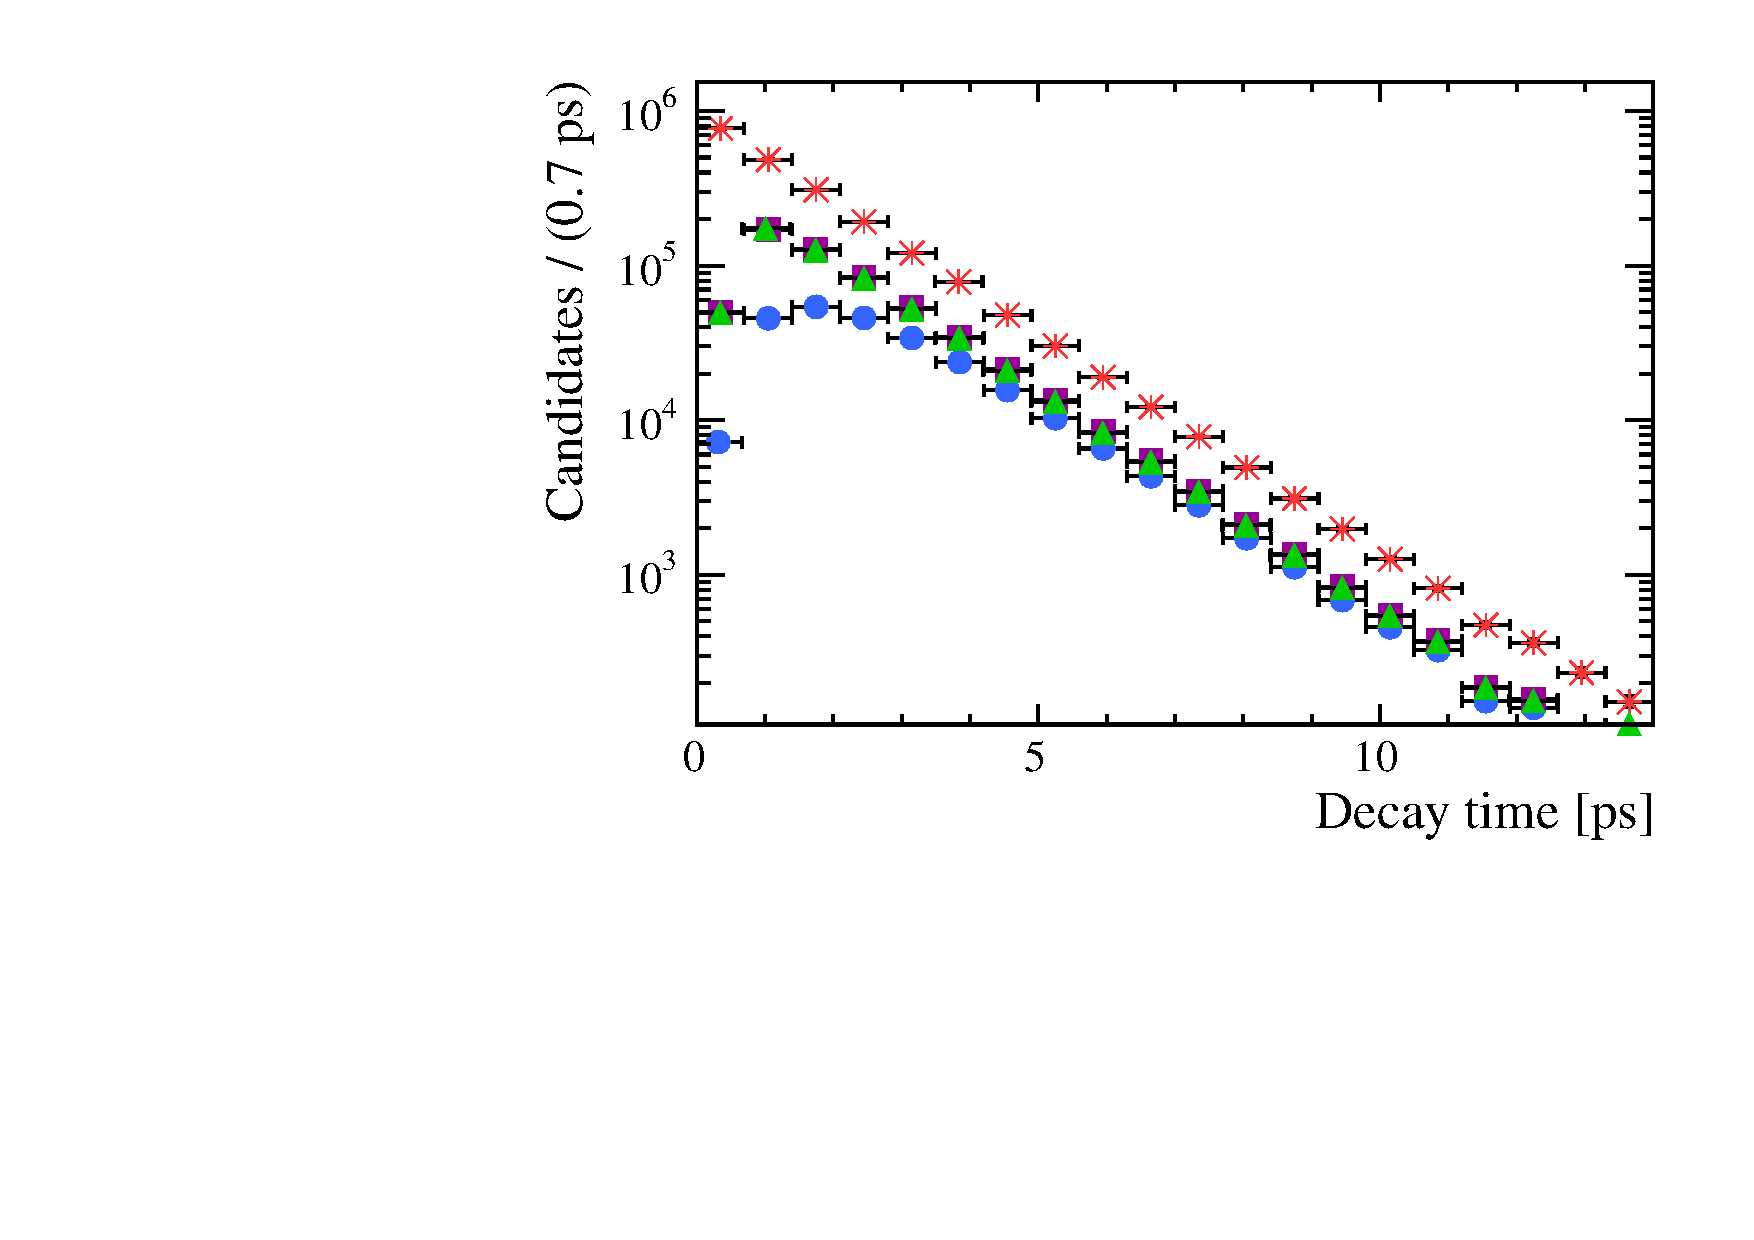
\includegraphics[width= \textwidth]{./Figs/LifetimeMeasurement/DT.pdf}
        %\caption{ }                                                                                                                    
        %\label{fig:BDTSsig}                                                                                                            
    \end{subfigure}
   ~ %add desired spacing between images, e. g. ~, \quad, \qquad, \hfill etc.                                                         
      %(or a blank line to force the subfigure onto a new line)                                                                         
    \begin{subfigure}[b]{0.48\textwidth}
       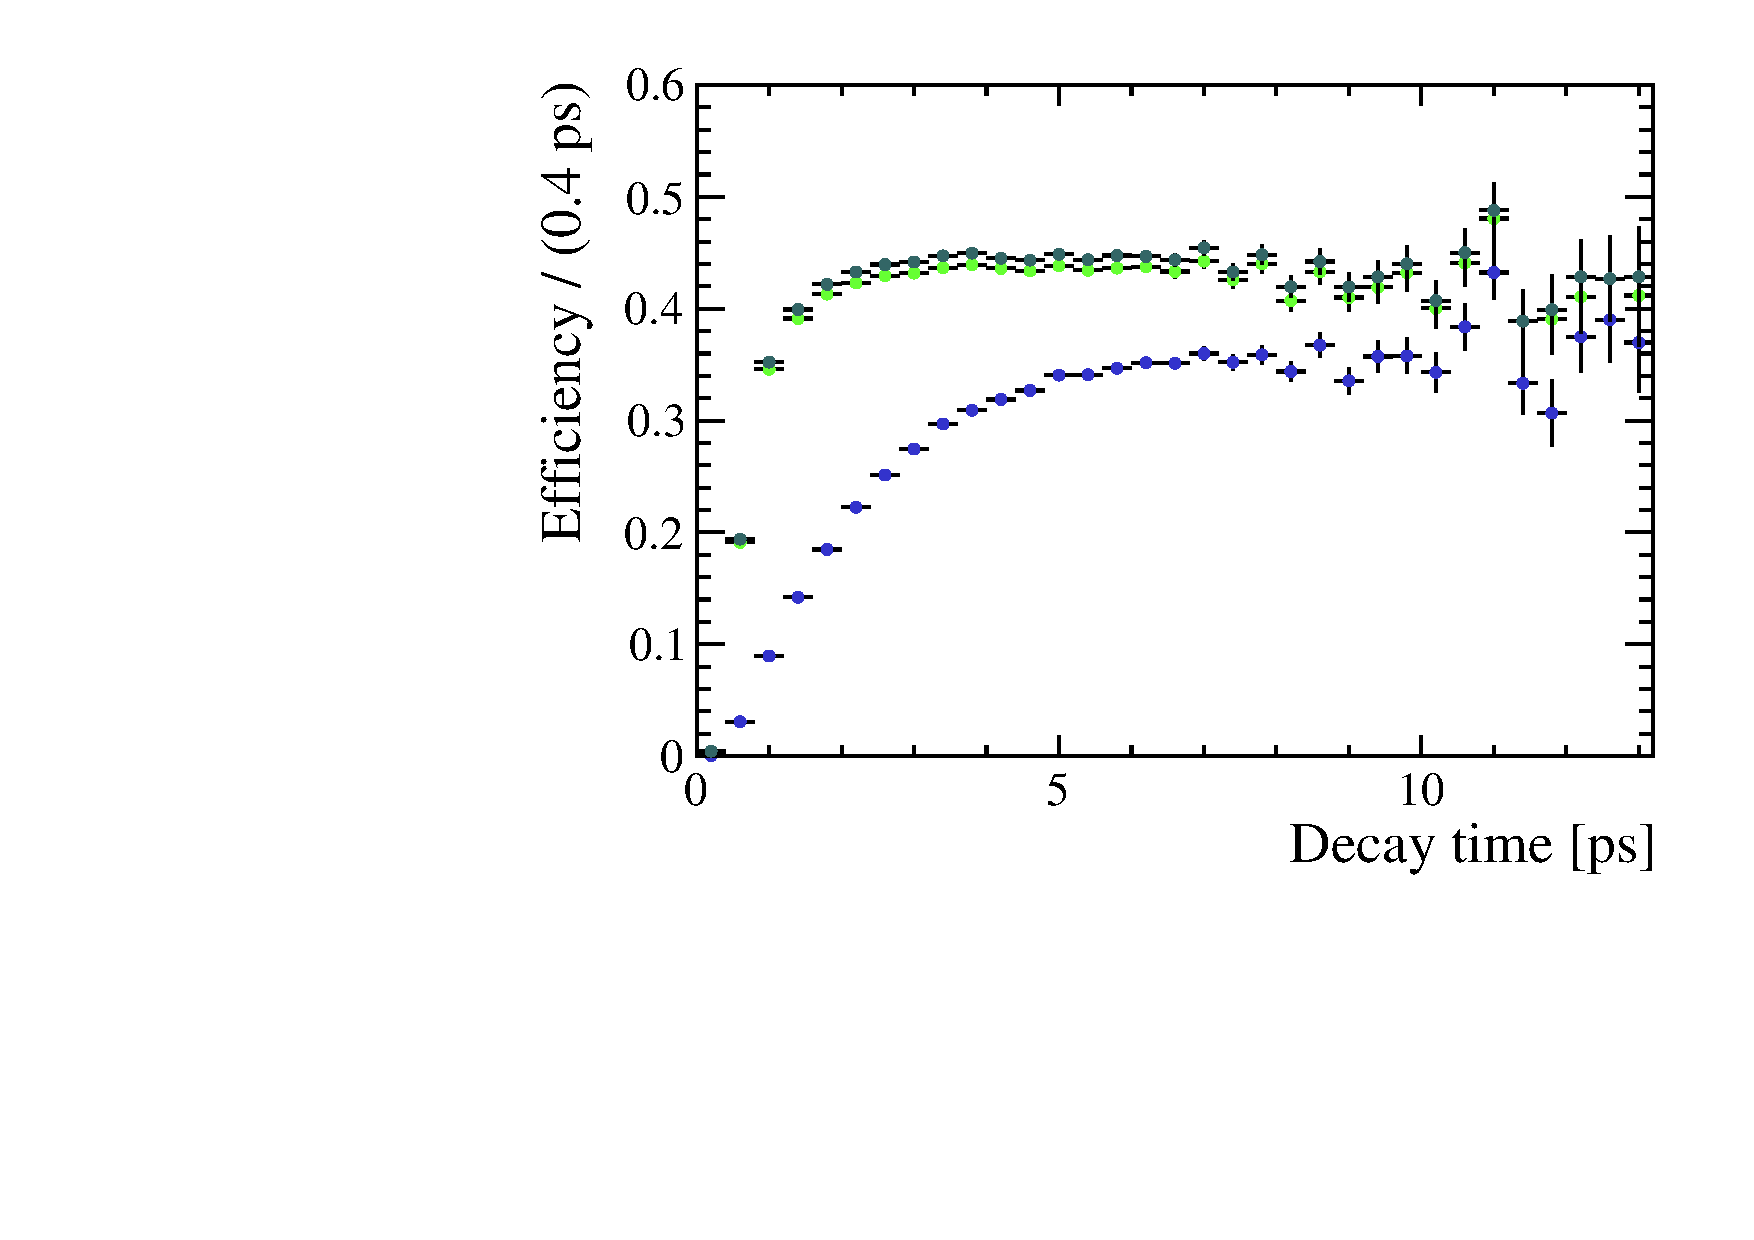
\includegraphics[width=\textwidth]{./Figs/LifetimeMeasurement/Accpt.pdf}
      %  \caption{ }                                                                                                                    
     %   \label{fig:BDTSbkg}                                                                                                            
   \end{subfigure}
    \caption{Decay time distribution (left) and selection efficiency as a function of decay time (right) for 2012 \bsmumu simulated decays at different different stages of the selection process. The decay time distributions and efficiencies are shown for reconstructed decays that pass the trigger, stripping and pre-selection cuts (magenta squares), the decays that go on to pass PID requirements (green triangles) and decays that pass all selection requirement including the global BDT cut (blue circles). Also the decay time distribution is shown for all generated simulated decays (red stars).} %Hmm can’t see them all on the decay time dist! Perhaps separate trigger or add in more MC?
    \label{fig:accpteg}
\end{figure}

To measure the \bsmumu effective lifetime, the efficiency of the selection on \bsmumu decays as a function of decay time must be accurately modelled. The determination of $\epsilon(t)$ for \bsmumu decays is described in Section~\ref{sec:signalDTpdf}. Although the sPlot method used to measure the \bsmumu effective lifetime means that the decay time \pdfs of the backgrounds present in the data set are not needed, realistic  descriptions of the background decay time \pdfs are necessary for optimising the mass fit configuration. The background \pdfs used are described in Section~\ref{sec:bkgDTpdf}.


\subsection{\bsmumu}% decay time \pdf}
\label{sec:signalDTpdf}
The selection efficiency of \bsmumu decays as a function of decay time is modelled by an acceptance function and a range of different models were investigated. The model that described the \bsmumu decay time efficiency best was the parametrised acceptance used in reference~\cite{LHCb:2011ab} 
\begin{equation}
\epsilon(t) = \frac{[a(t - t_{0}]^{n}}{1 + a(t - t_{0}]^{n}},
\label{eq:accpt}
\end{equation}
where $t$ is the decay time, $t_0$ the shortest decay time allowed for the function and $a$ and $n$ are parameters to be determined.  was found to best describe the \bsmumu decay time efficiency. The acceptance function parameters are taken from a fit to simulated \bsmumu decays and are fixed in the fit to data. The parameters could not be determined from data because there are too few \bsmumu decays in data and the efficiency distribution of the more abundant \bhh decays after the selection is quite different to that of \bsmumu. A systematic uncertainty describing how well the acceptance function is understood is detailed in Section~\ref{sec:accptsyst}. The decay time efficiency for each year of data taking is slightly different therefore simulated decays from each year of data taking must be used to determine the acceptance parameters.


In general simulated decays model distributions in data reasonably well, however the number of tracks present in an event are not well modelled in the simulation. %The isolation variables used in the global BDT depend on the number of track in an event and the isolation variables are also correlated with the decay time of the \bs. 
Although the \bsmumu decay time distribution does not depend on the number of tracks present in the event, the isolation criteria used in the global BDT do. Therefore, the selection efficiency as a function of decay time depends on the number of tracks in the event and cannot be accurately described by simulated decays alone. To overcome this the number of tracks in an event for simulated \bsmumu decays are weighted using information from the number of tracks per event for \bdkpi decays in both data and simulation. 

The selection requirements listed in Table~\ref{tab:fullpreselectionEL} are used to identify \bdkpi decays in data and simulation but importantly the global BDT cut is not applied. The DLL$_{K\pi}$ variable is used to separate \bdkpi decays from other \bhh decays in data and the loose trigger requirements used for the branching fraction analysis are applied to data and simulation to keep a high trigger efficiency\footnote{The Hlt2Phys Dec trigger decision was not correctly implemented in 2016 simulated decays, therefore the DEC decisions of a combination of trigger lines designed to select \bhh are used to emulate the Hlt2Phys DEC trigger decision. The trigger lines are Hlt2Topo2BodyDecision, Hlt2B2HH\_Lb2PPiDecision, Hlt2B2HH\_Lb2PKDecision Dec, Hlt2B2HH\_B2PiPiDecision, Hlt2B2HH\_B2PiKDecision, Hlt2B2HH\_B2KKDecision and Hlt2B2HH\_B2HHDecision. These trigger lines are applied to both data and simulated decays.}. The same requirements are applied to simulated decays. The distribution of the number of tracks present in events containing \bdkpi decays is obtained from data by performing a maximum likelihood fit to the \bd mass distribution and extracting sWeights. The distribution of the weighted number of tracks per event in data is compared with the distribution in simulated \bdkpi decays. The mass fits to \bdkpi decays in data are shown in Figure~\ref{fig:ntracksmassifts} and the normalised distributions of the number of tracks per event in weighted data and simulated decays are shown in Figure~\ref{fig:nTracksMCDataComp}. Each year of data taking is kept separate and the same simulation version is used for \bdkpi simulated decays as available for \bsmumu decays.



\begin{figure}[t!]
  \centering
    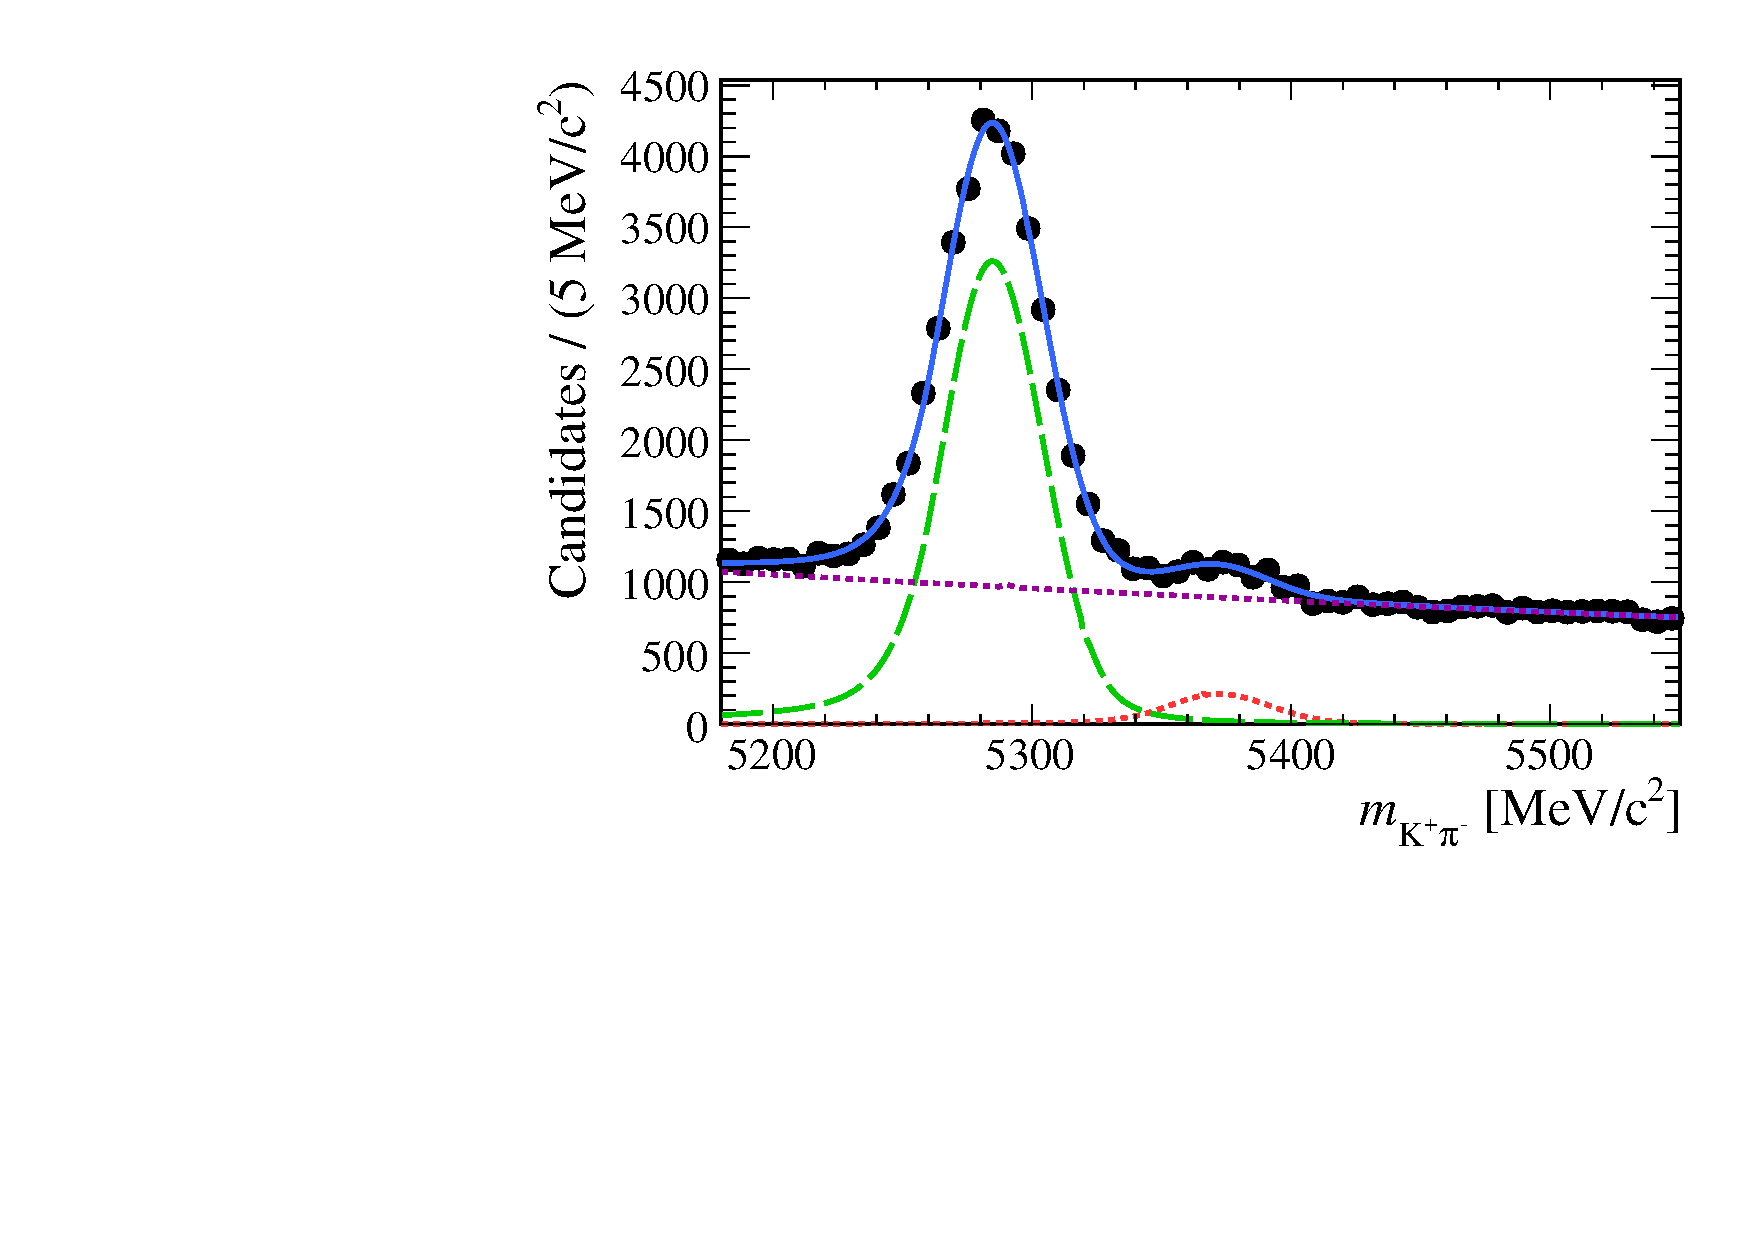
\includegraphics[width=0.49\textwidth]{./Figs/LifetimeMeasurement/Bd2KPi_2011_mass_fit.pdf}
    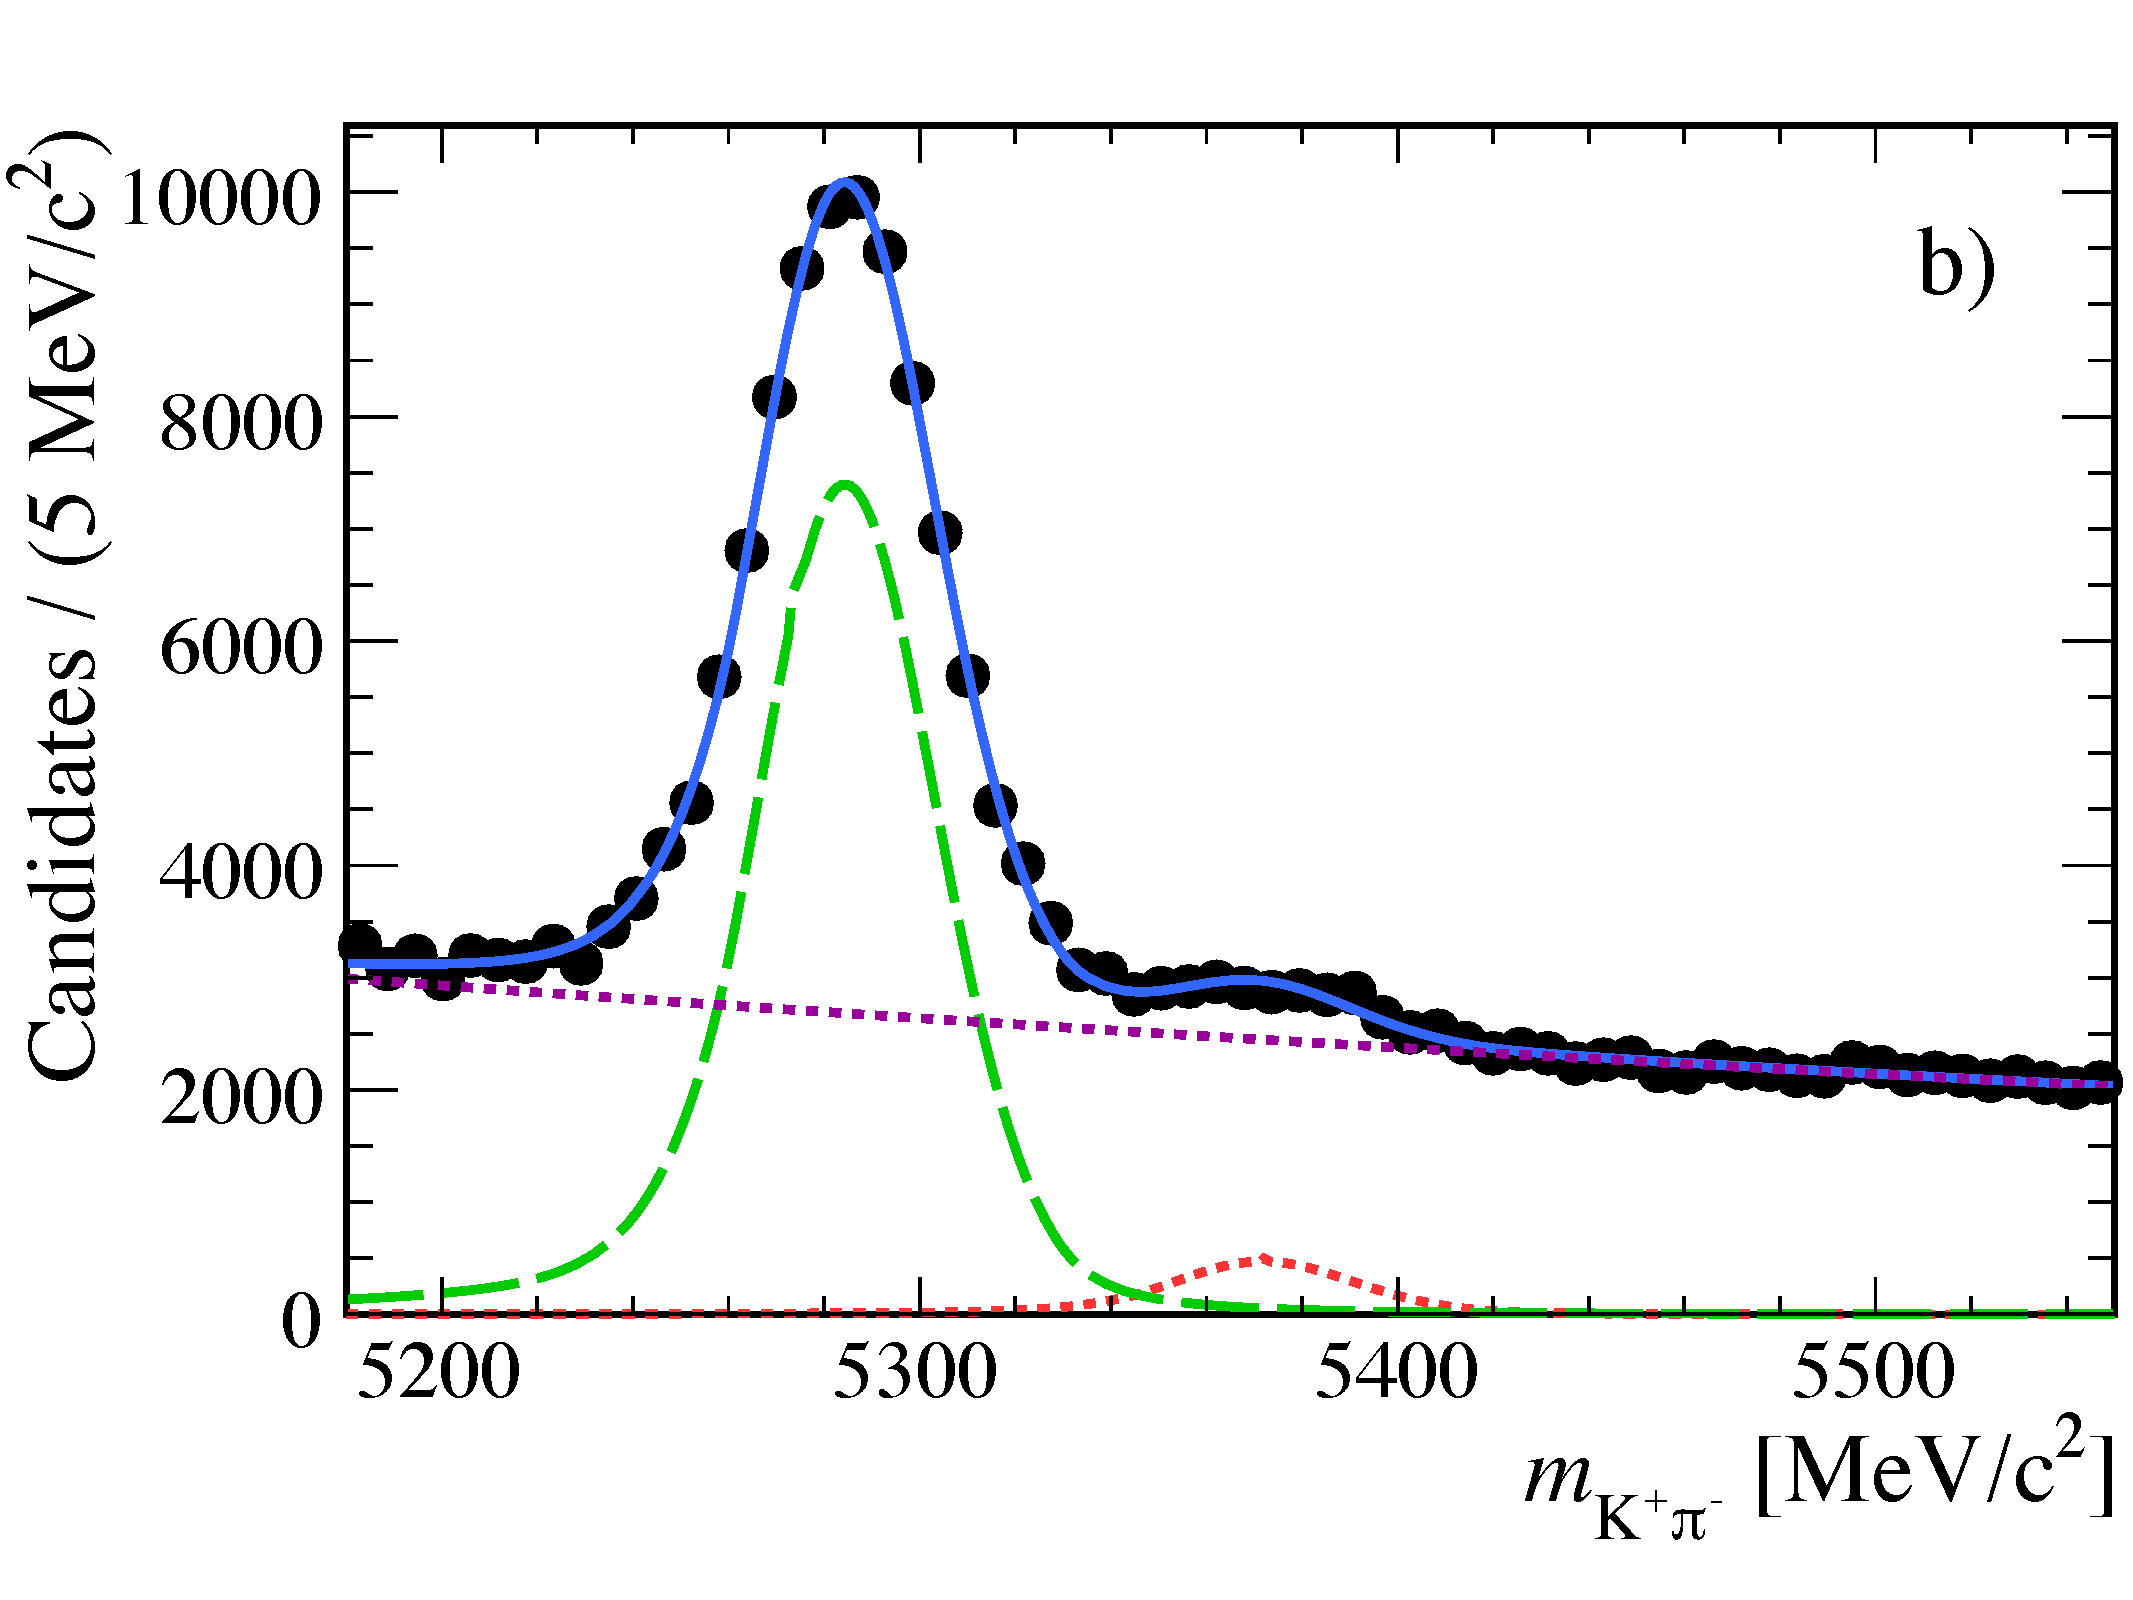
\includegraphics[width=0.49\textwidth]{./Figs/LifetimeMeasurement/Bd2KPi_2012_mass_fit.pdf}
    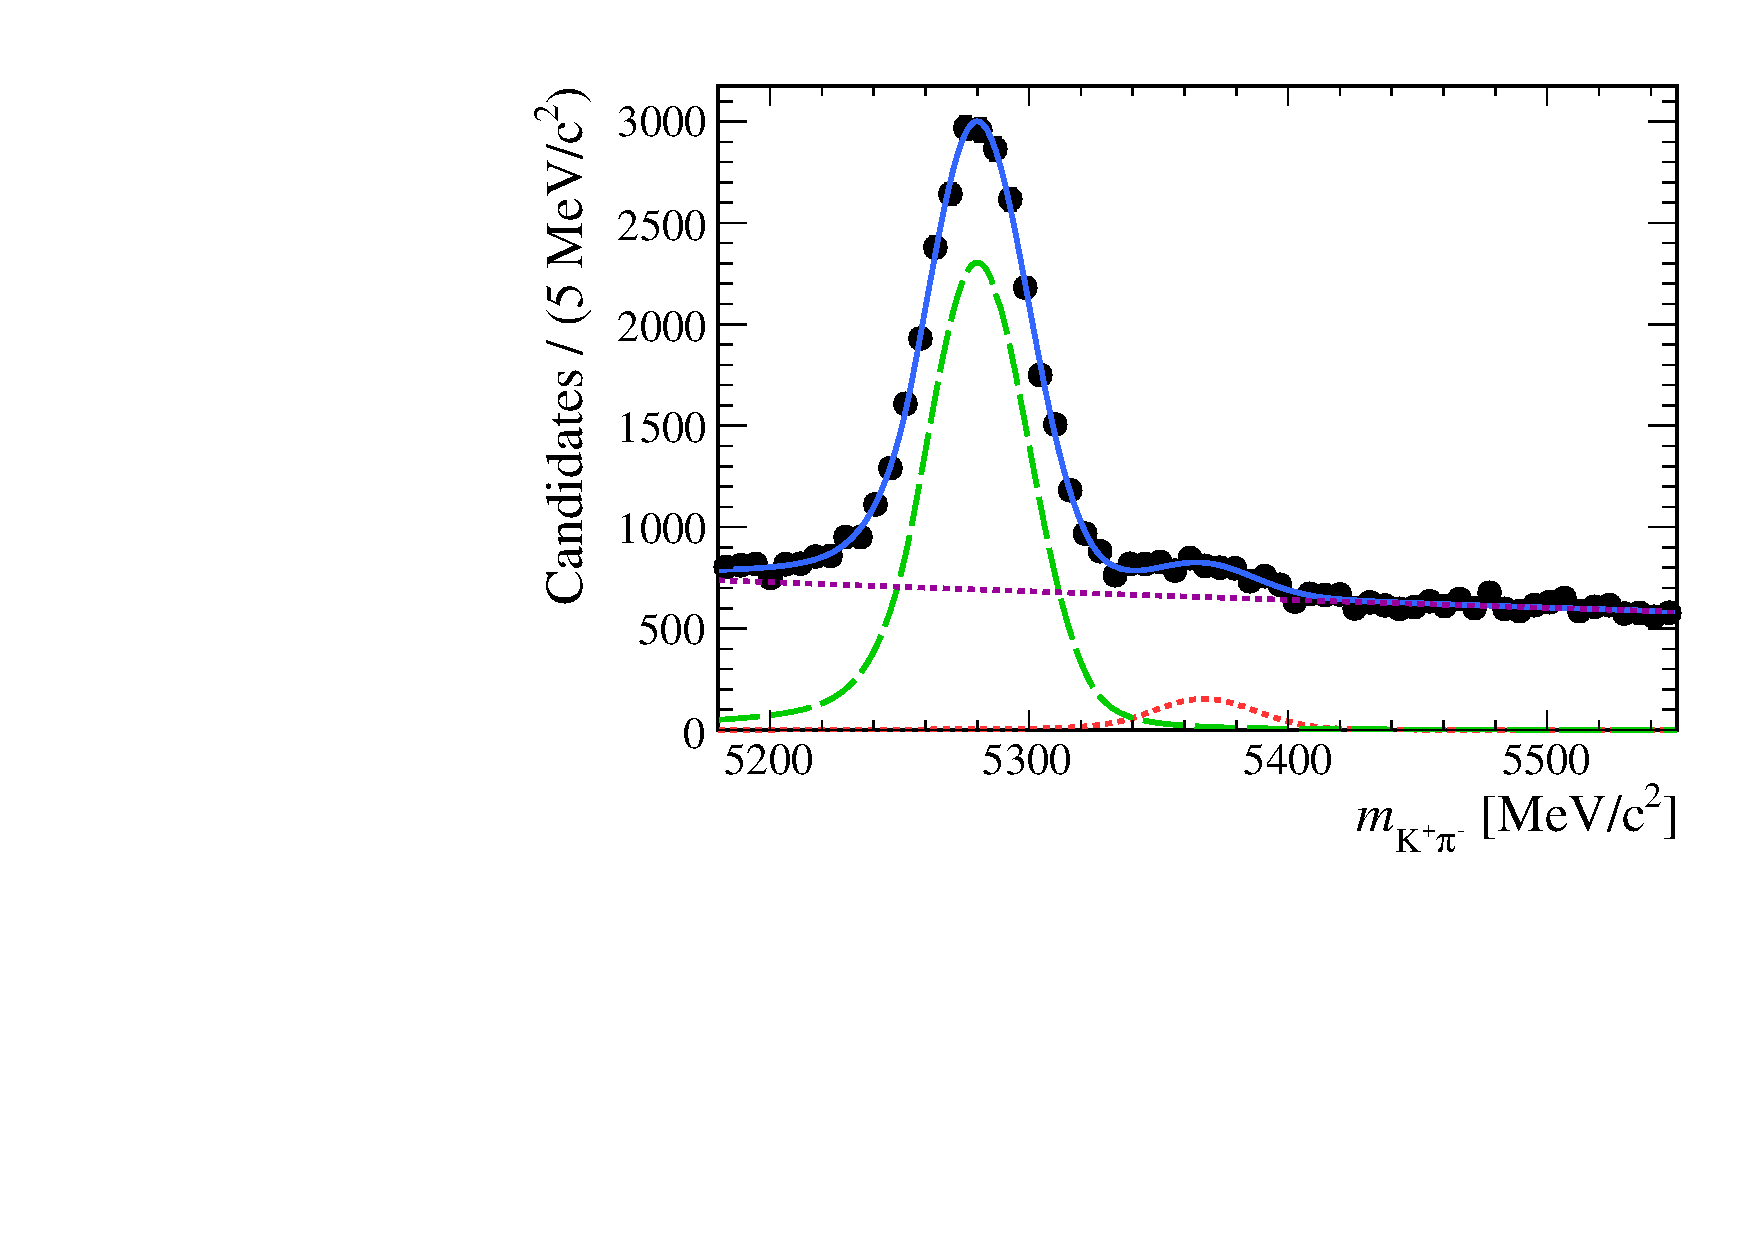
\includegraphics[width=0.49\textwidth]{./Figs/LifetimeMeasurement/Bd2KPi_2015_mass_fit.pdf}
    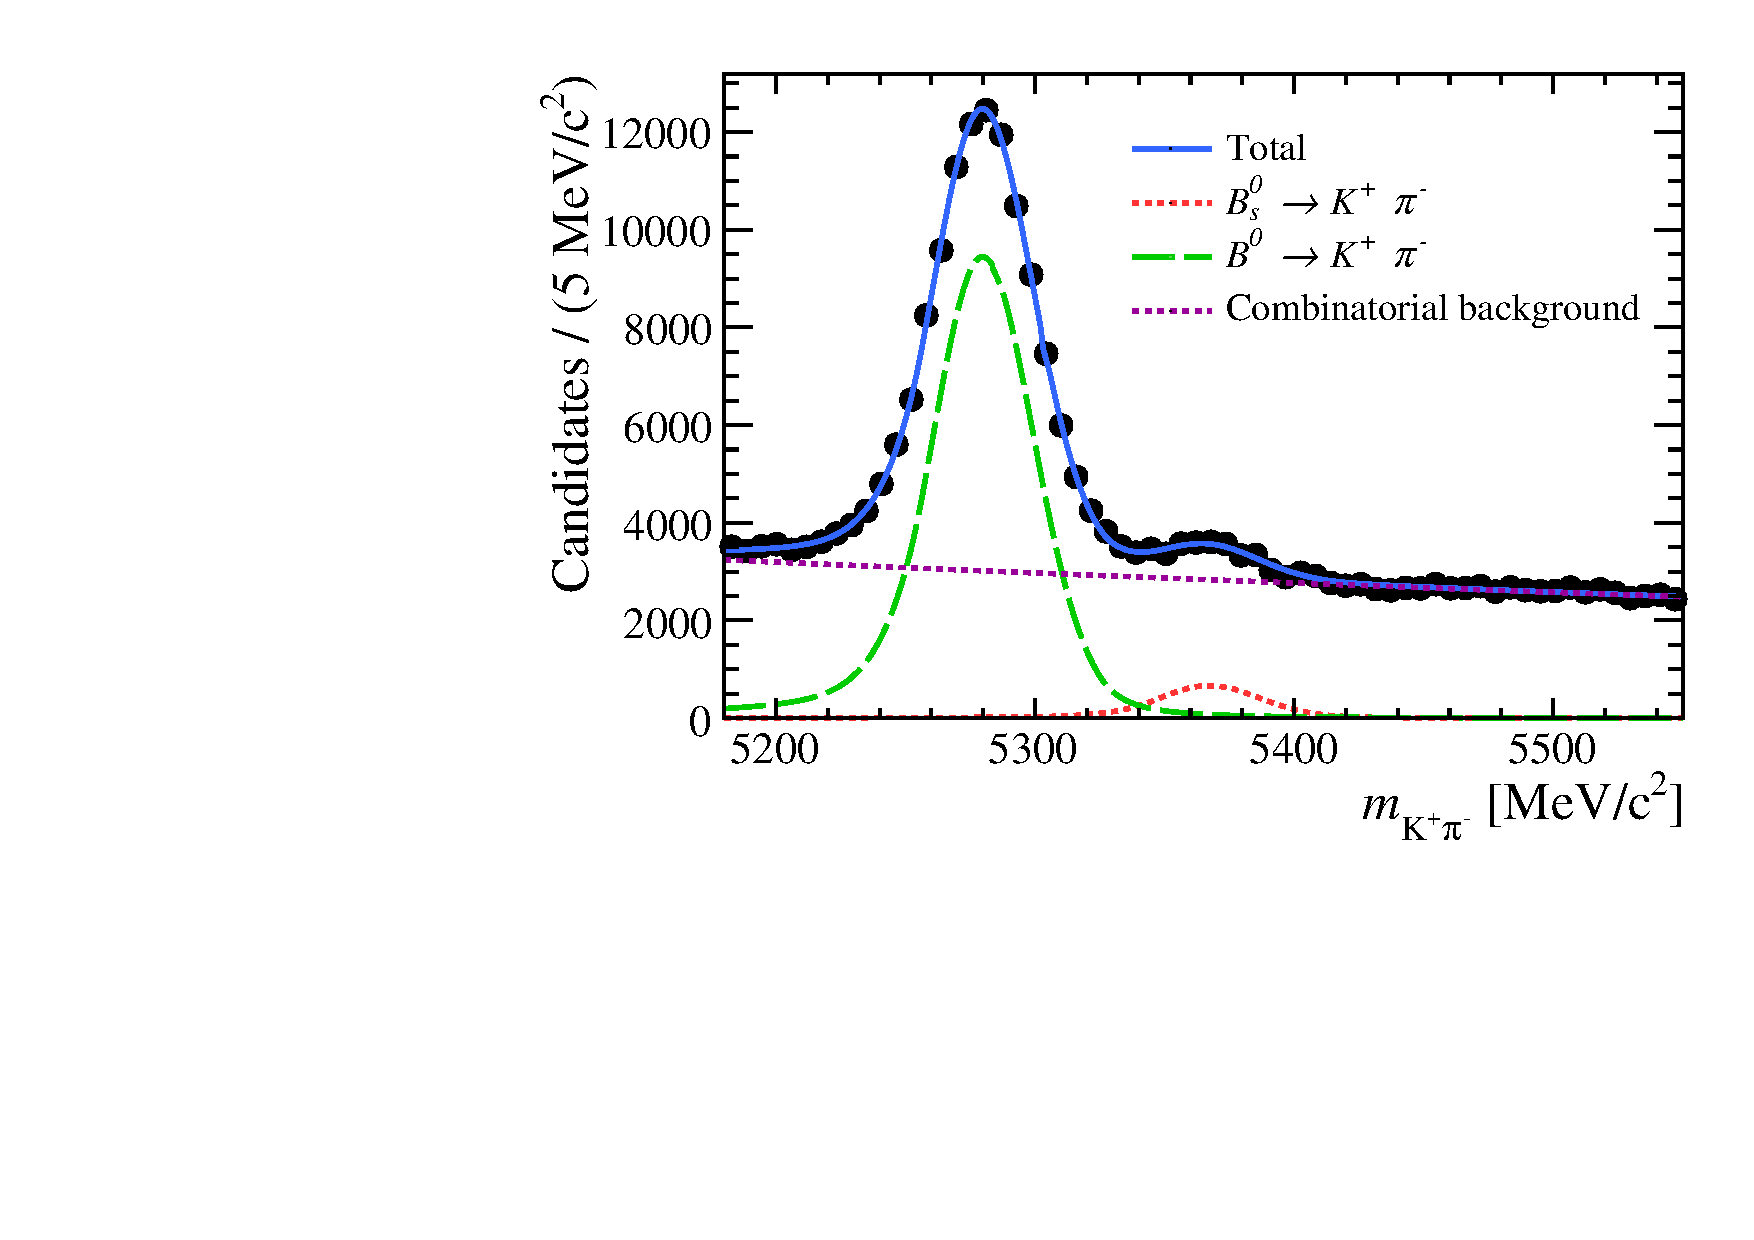
\includegraphics[width=0.49\textwidth]{./Figs/LifetimeMeasurement/Bd2KPi_2016_mass_fit.pdf}
  \caption{Maximum likelihood fits to the mass distribution of \bdkpi candidates in 2011 (top left), 2012 (top right), 2015 (bottom left) and 2016 (bottom right) data. The mass \pdf includes components for \bdkpi (green), \bskpi (red) and combinatorial background (purple).}
  \label{fig:ntracksmassifts}
\end{figure}
\FloatBarrier




The distributions of the number of tracks per event for \bdkpi decays in data and simulated decays are used to weight \bdkpi decays so that the distribution in simulation matches that in data. The weights are evaluated by taking the ratio of the normalised histograms in Figure~\ref{fig:nTracksMCDataComp} for the number of tracks per event in data and simulation for each year. The affect on the decay time distribution of using these weights and then applying the global BDT cut is shown in Figure~\ref{fig:BdToKpi_weightDecayTime} for the simulated \bdkpi decays. The difference between the decay time distributions with and without the weights is not large but clearly noticeable at low decay times where the change in selection efficiency is greatest. 


\begin{figure}[tbp]
  \centering
    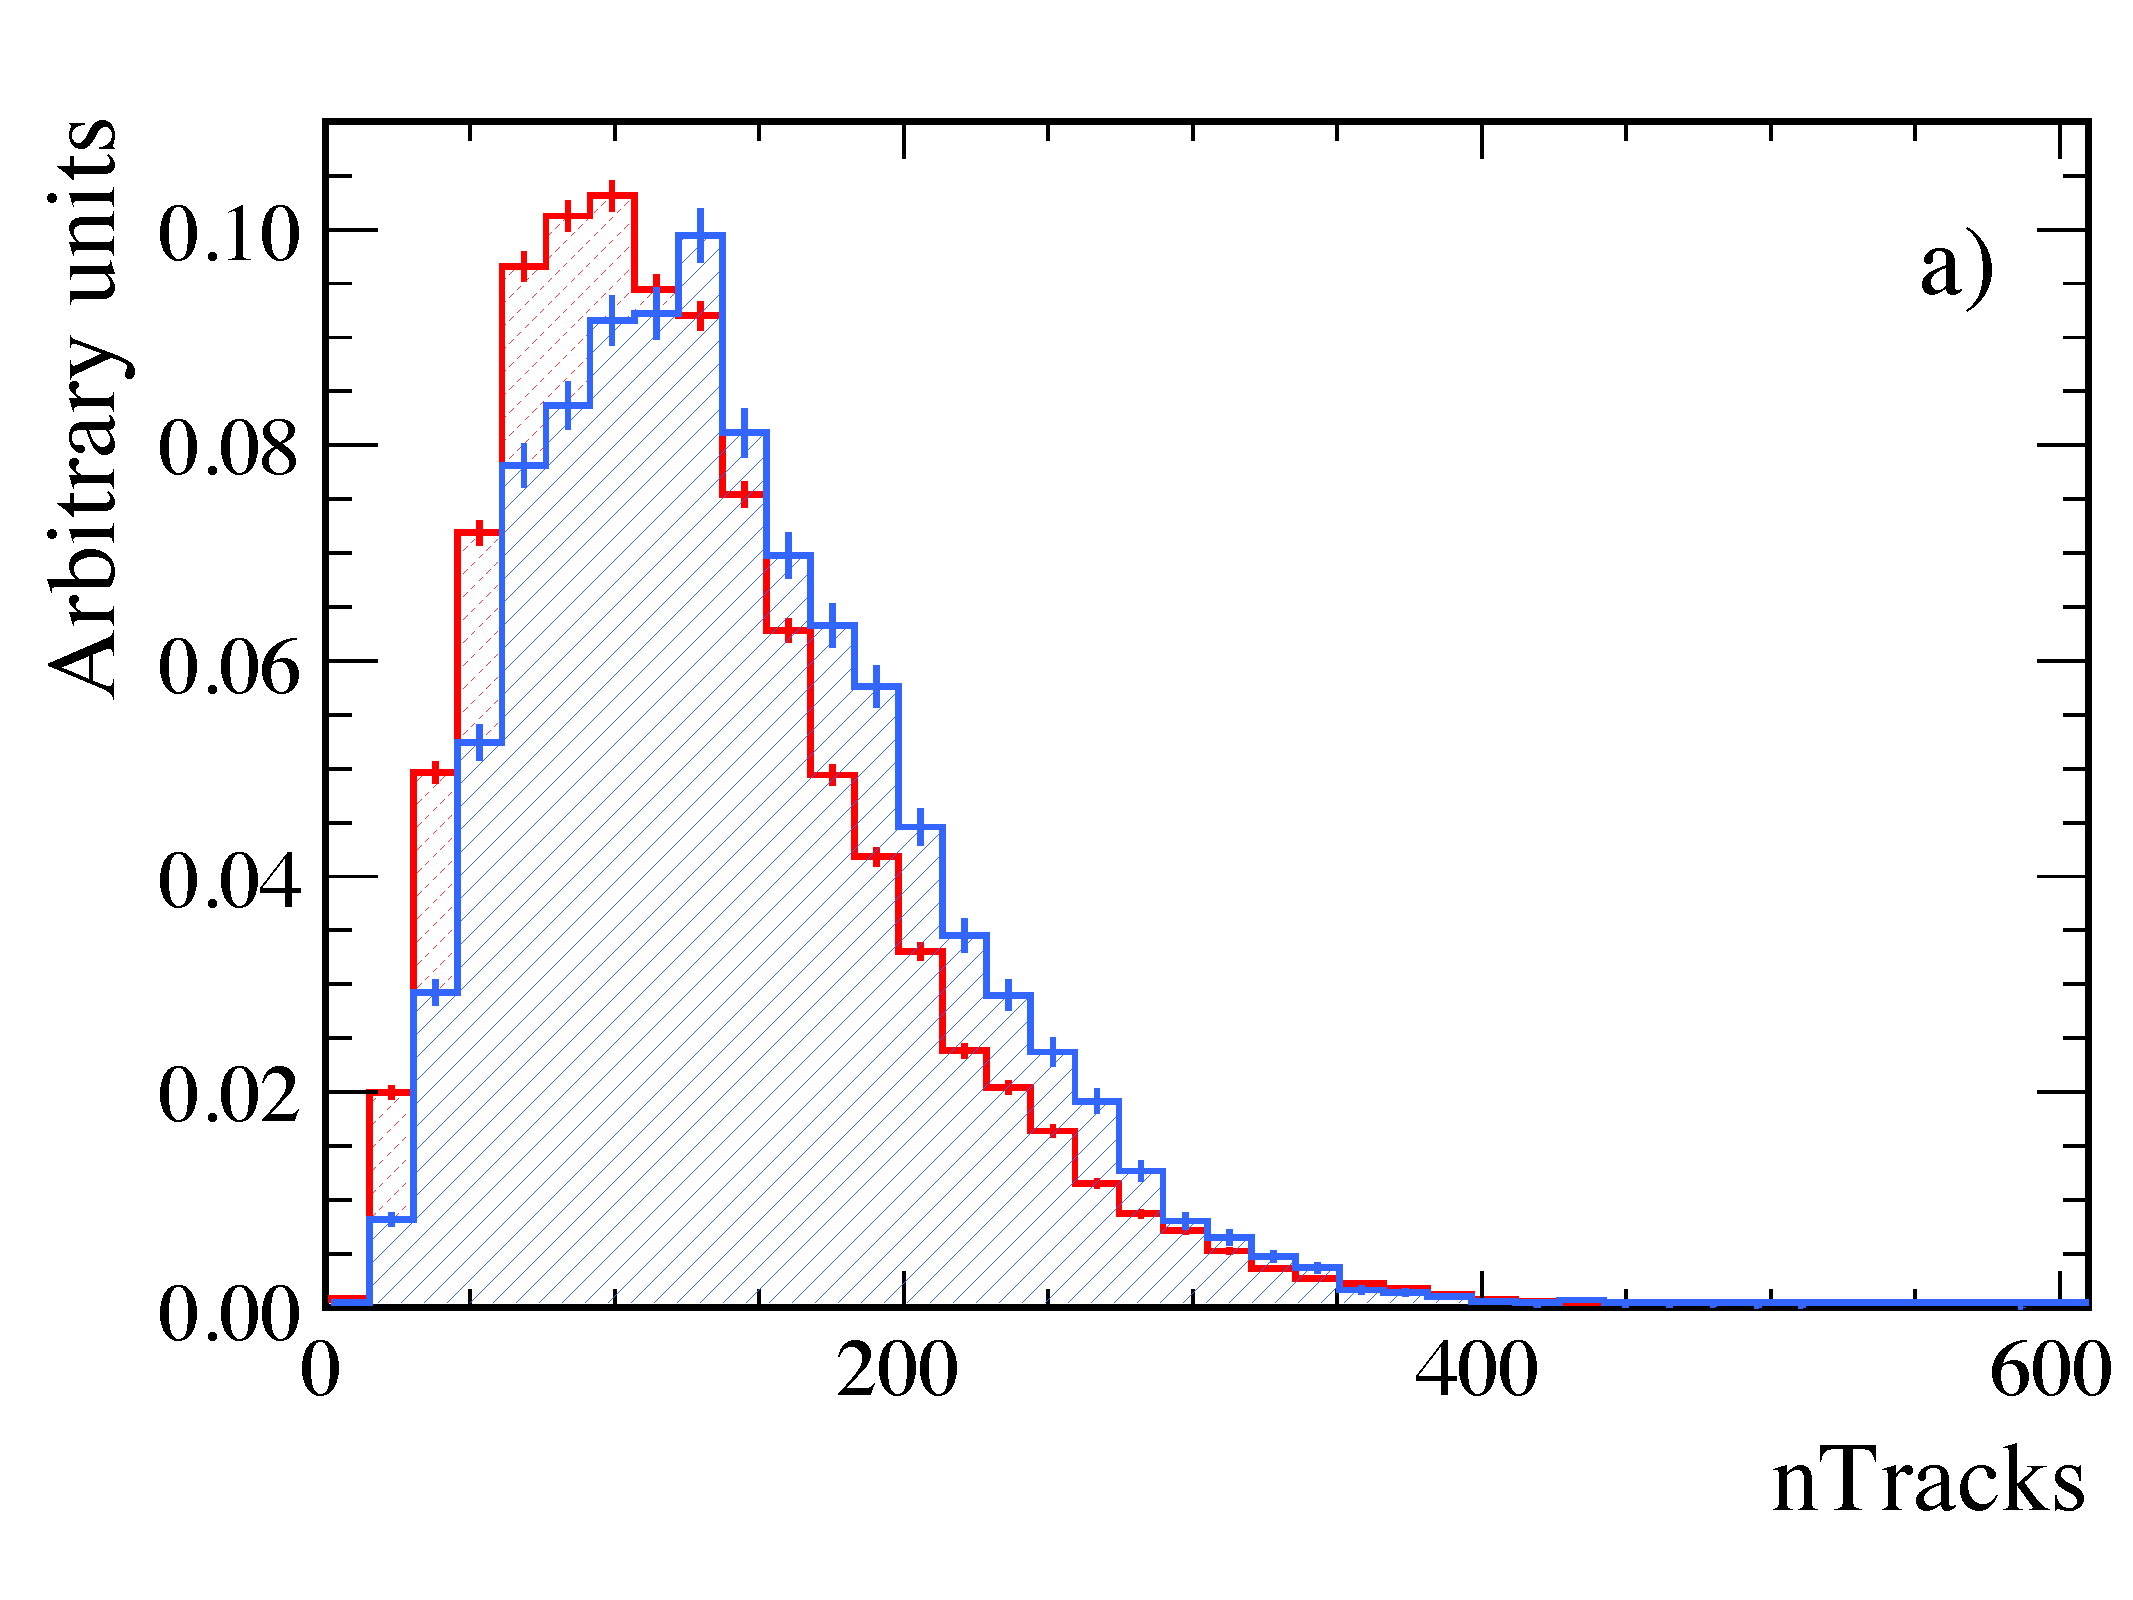
\includegraphics[width=0.49\textwidth]{./Figs/LifetimeMeasurement/Bd2KPi_2011_data_MC_nTracks.pdf}
    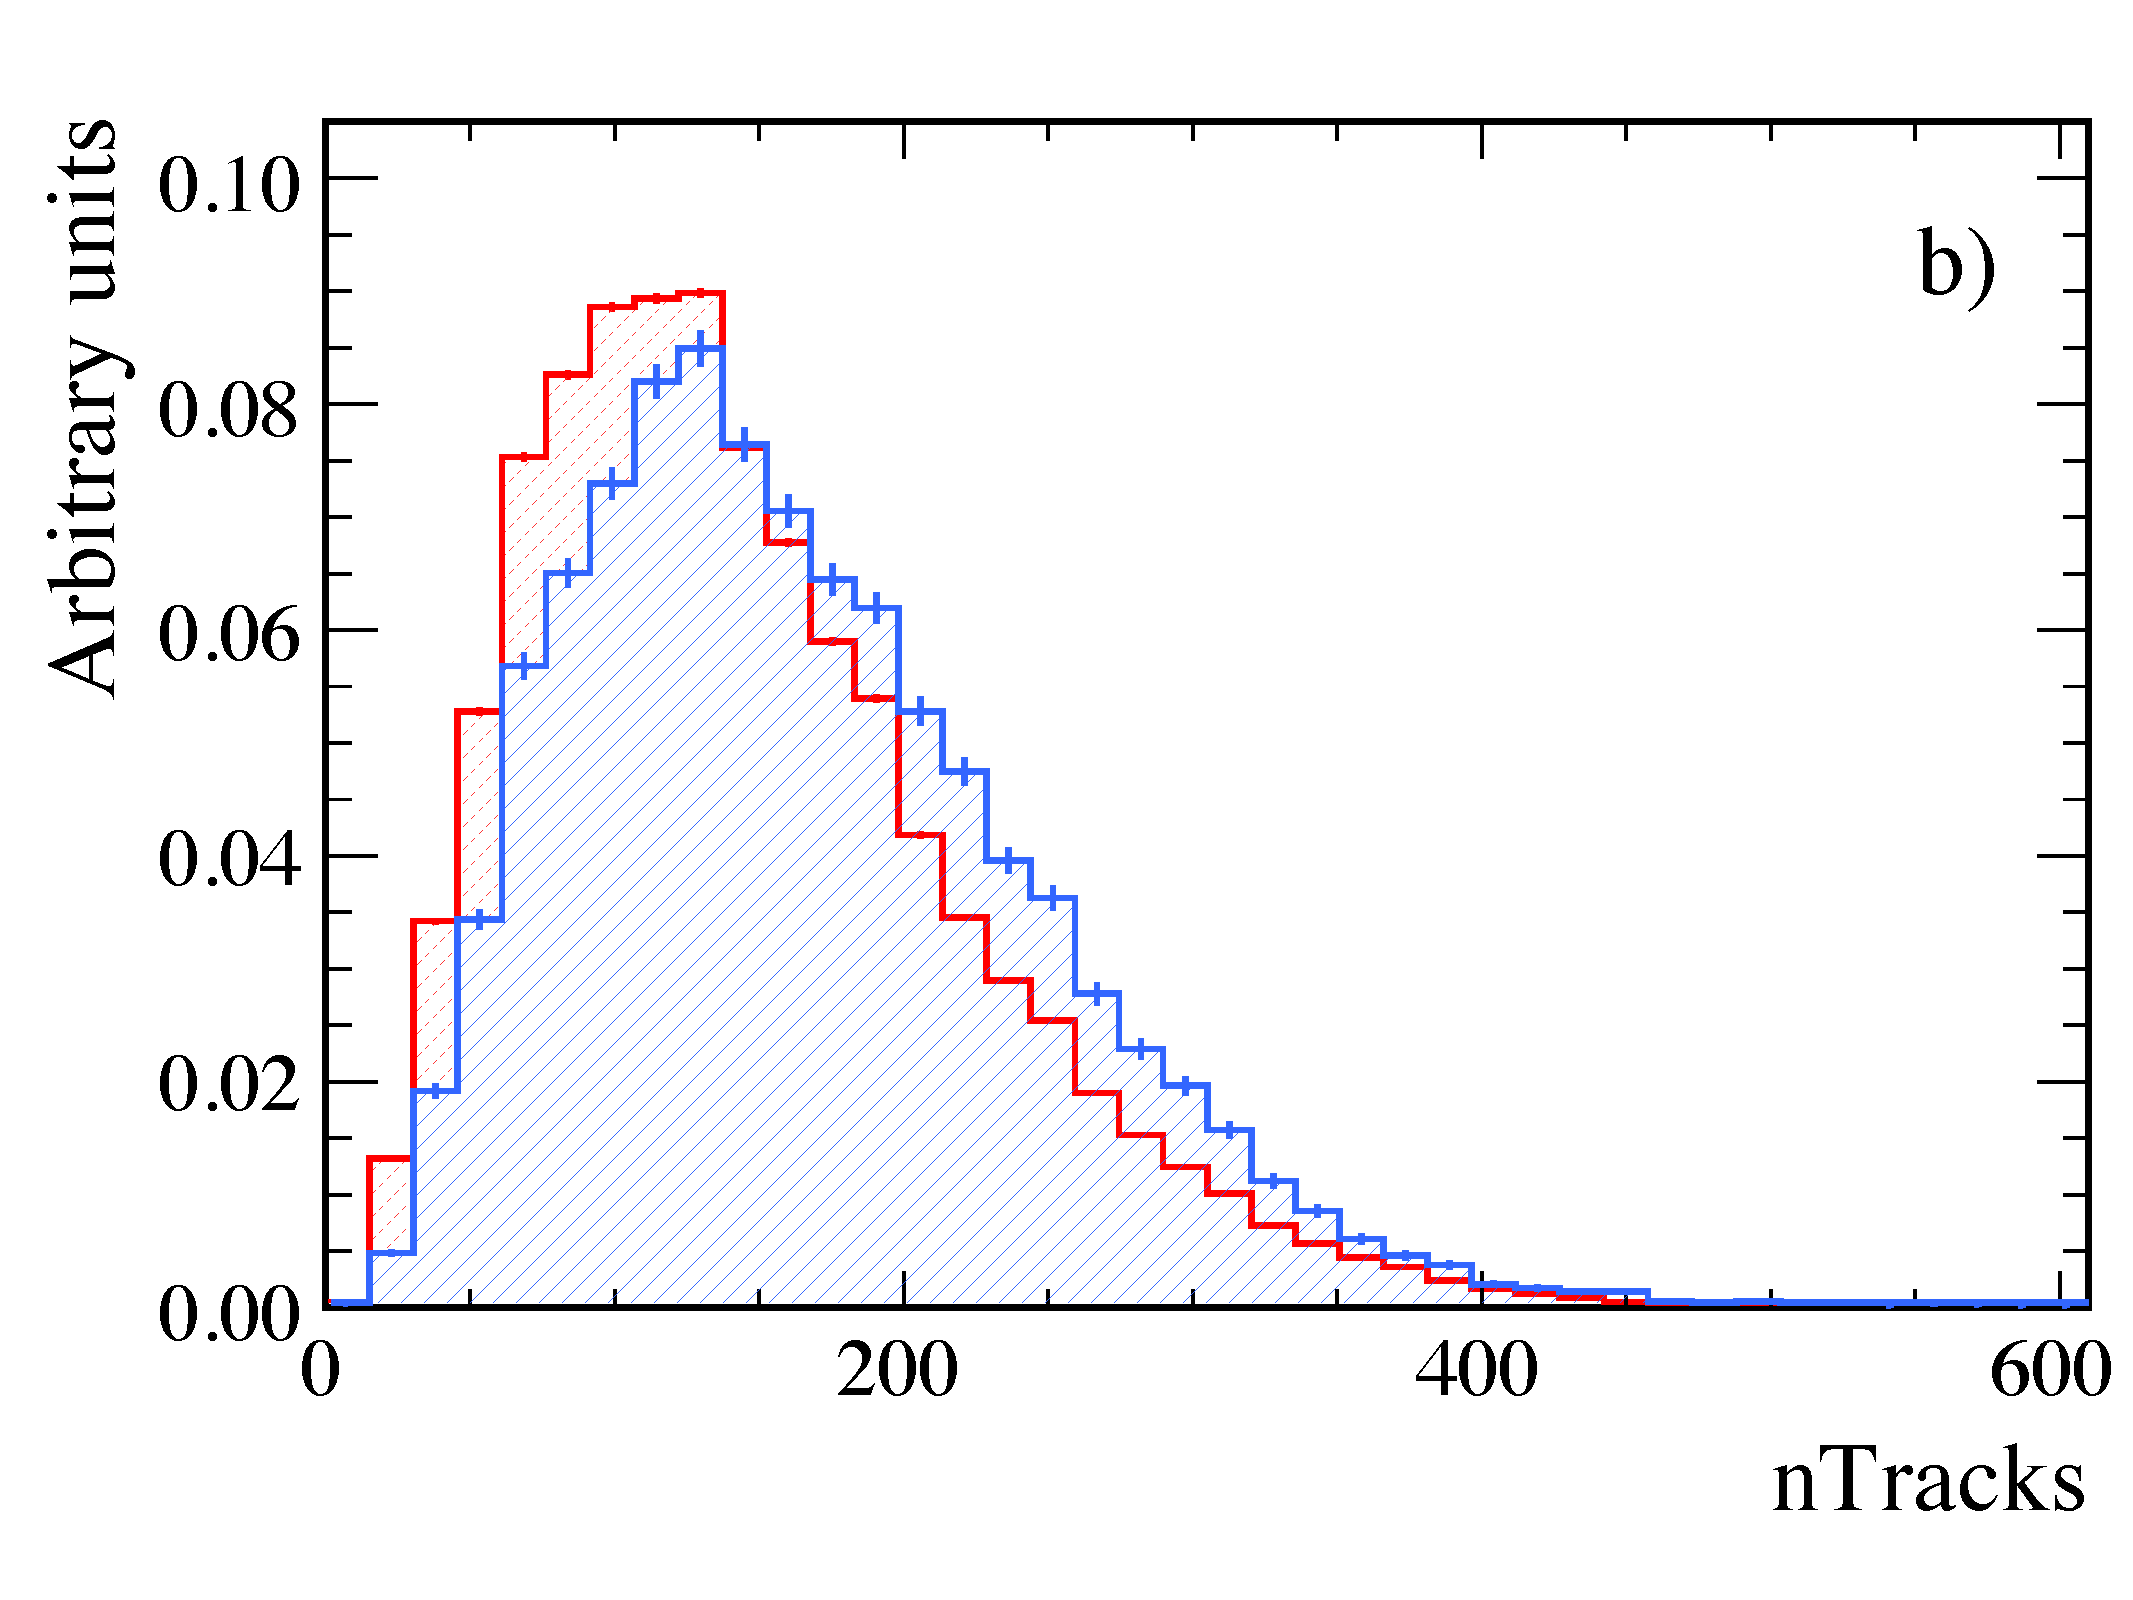
\includegraphics[width=0.49\textwidth]{./Figs/LifetimeMeasurement/Bd2KPi_2012_data_MC_nTracks.pdf}
    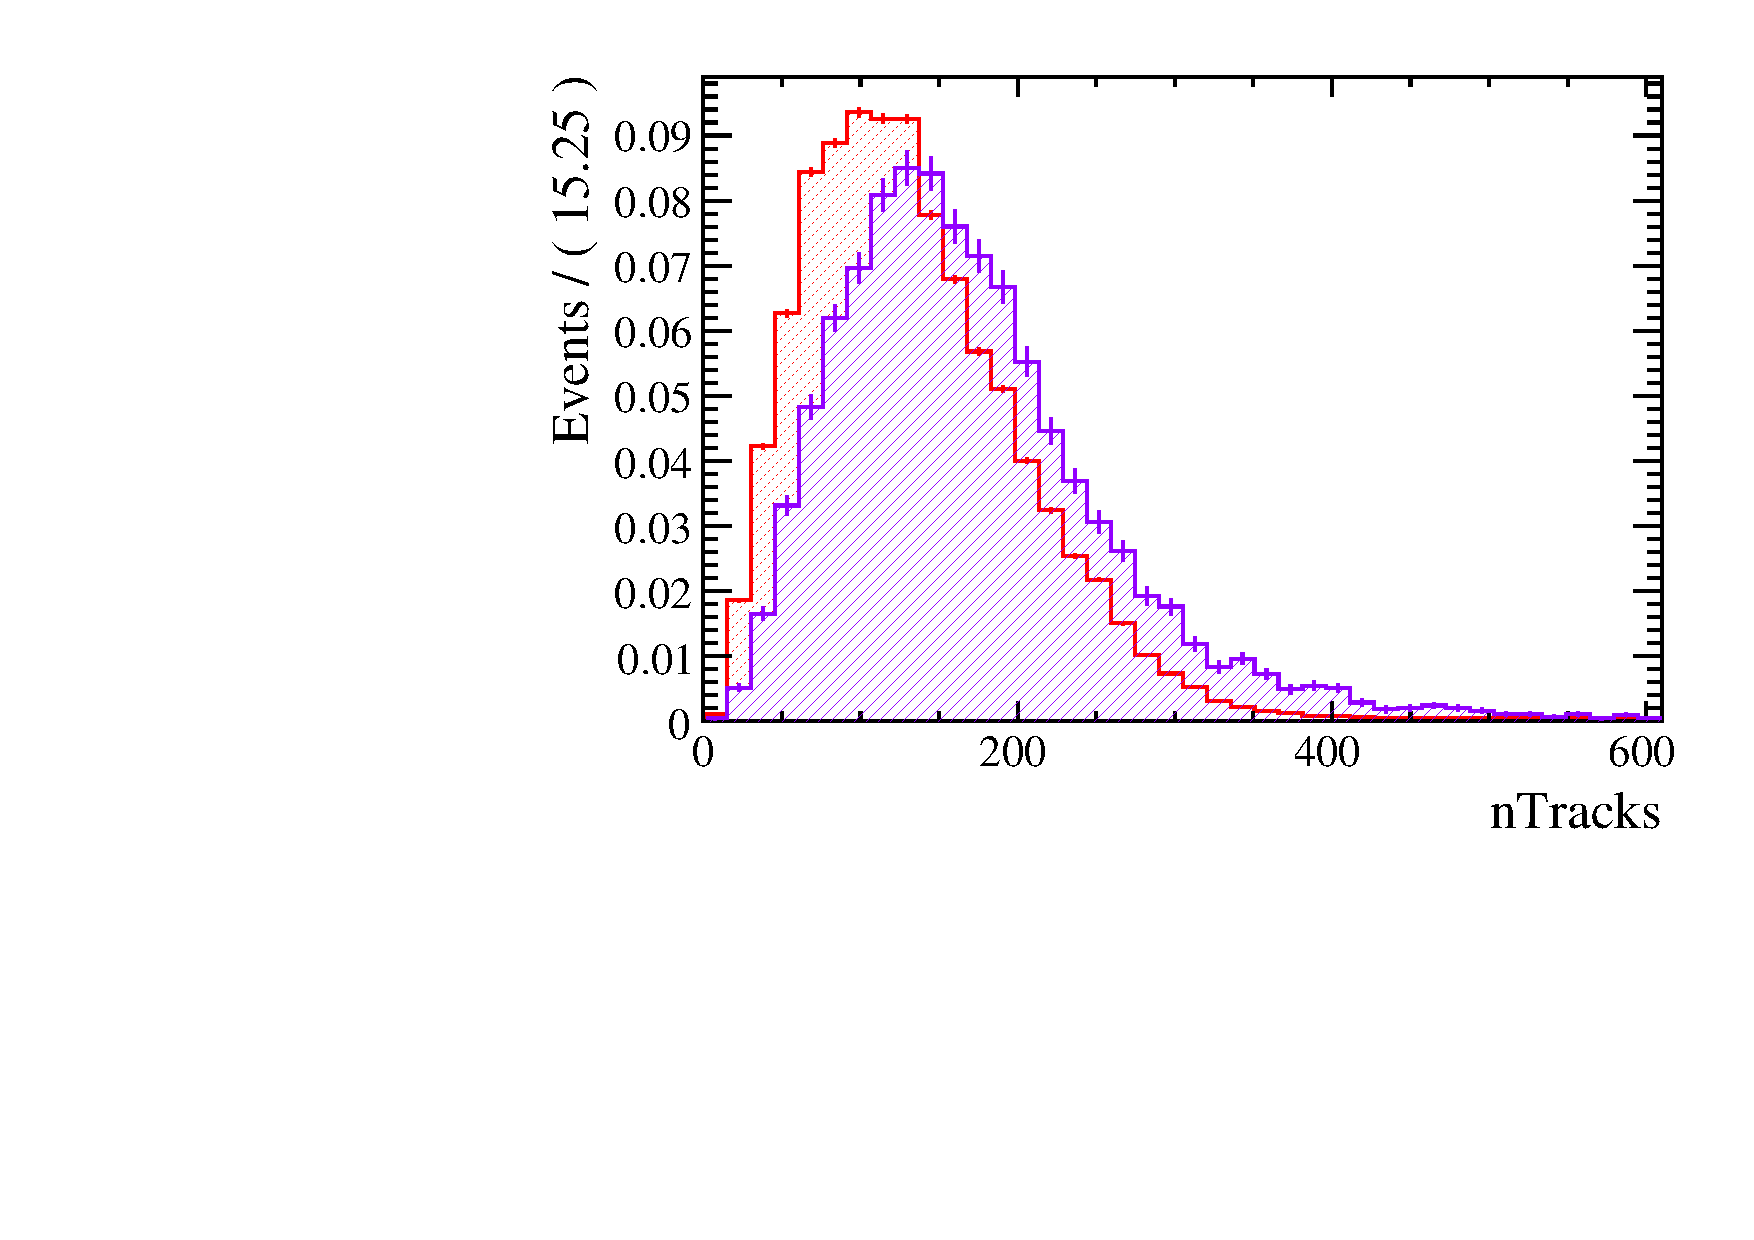
\includegraphics[width=0.49\textwidth]{./Figs/LifetimeMeasurement/Bd2KPi_2015_data_MC_nTracks.pdf}
    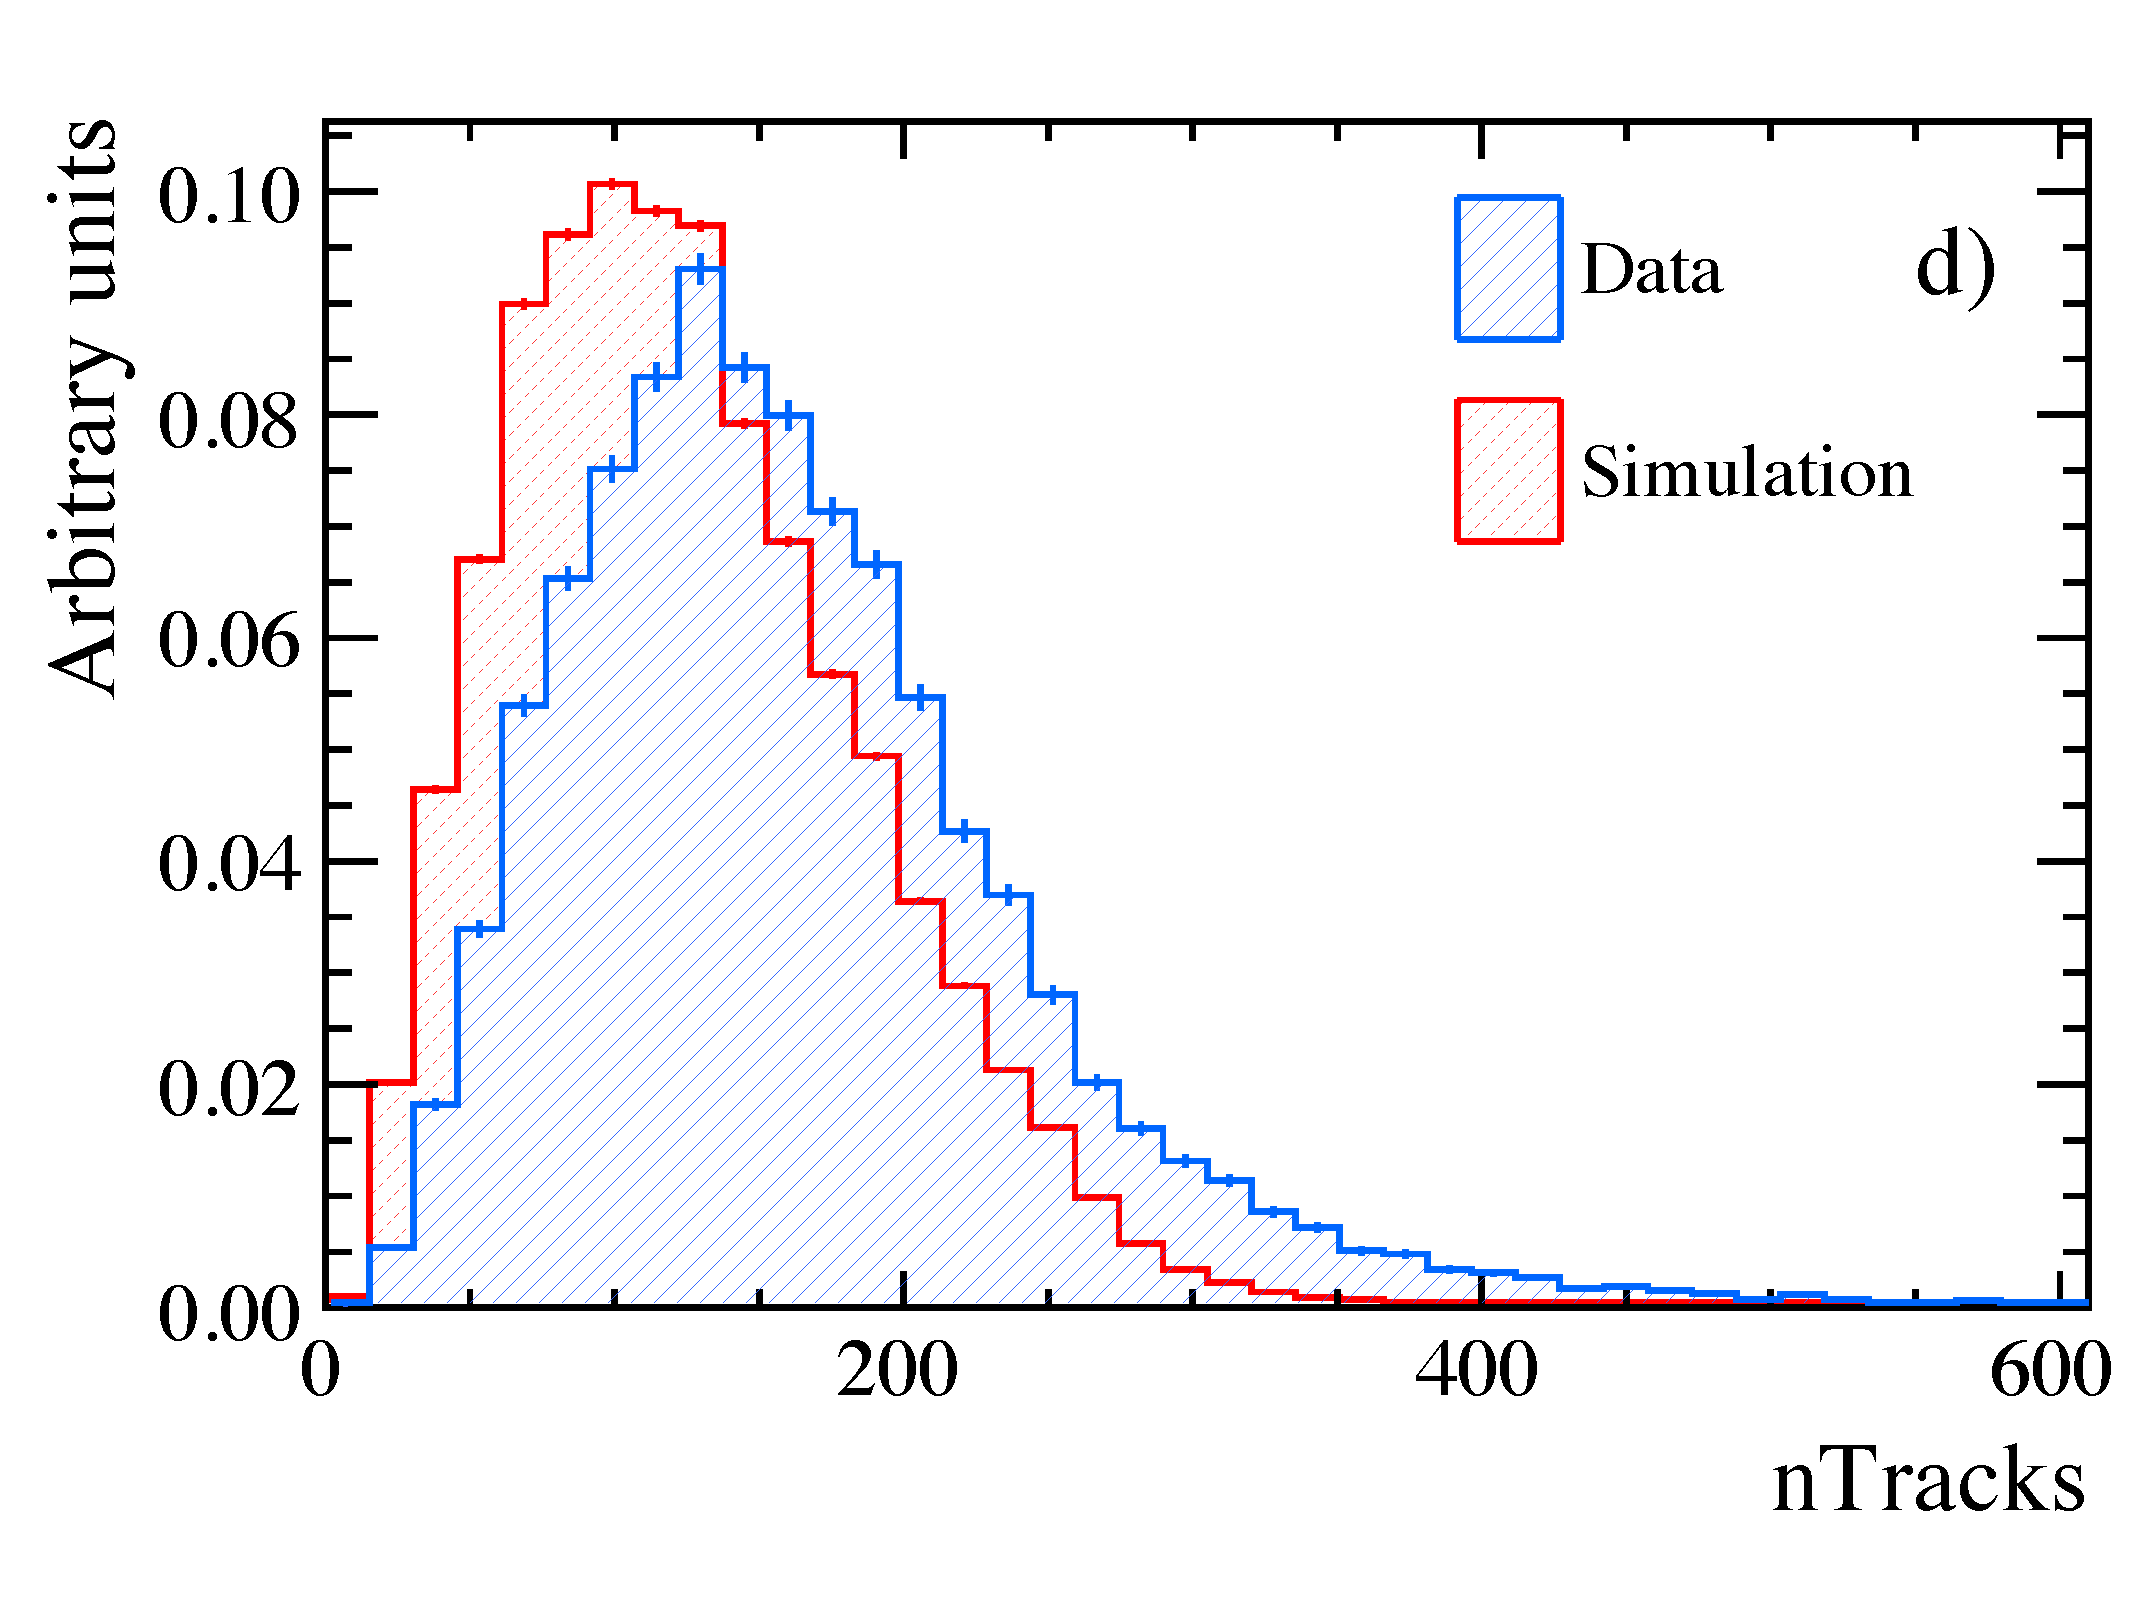
\includegraphics[width=0.49\textwidth]{./Figs/LifetimeMeasurement/Bd2KPi_2016_data_MC_nTracks.pdf}
  \caption{Normalised histograms of the number of tracks per event in simulated \bdkpi decays and weighted \bdkpi decays in data for 2011 (top left), 2012 (top right), 2015 (bottom left) and 2016 (bottom right) data. }
  \label{fig:nTracksMCDataComp}
\end{figure}
\FloatBarrier
\begin{figure}[tbp]
  \centering
    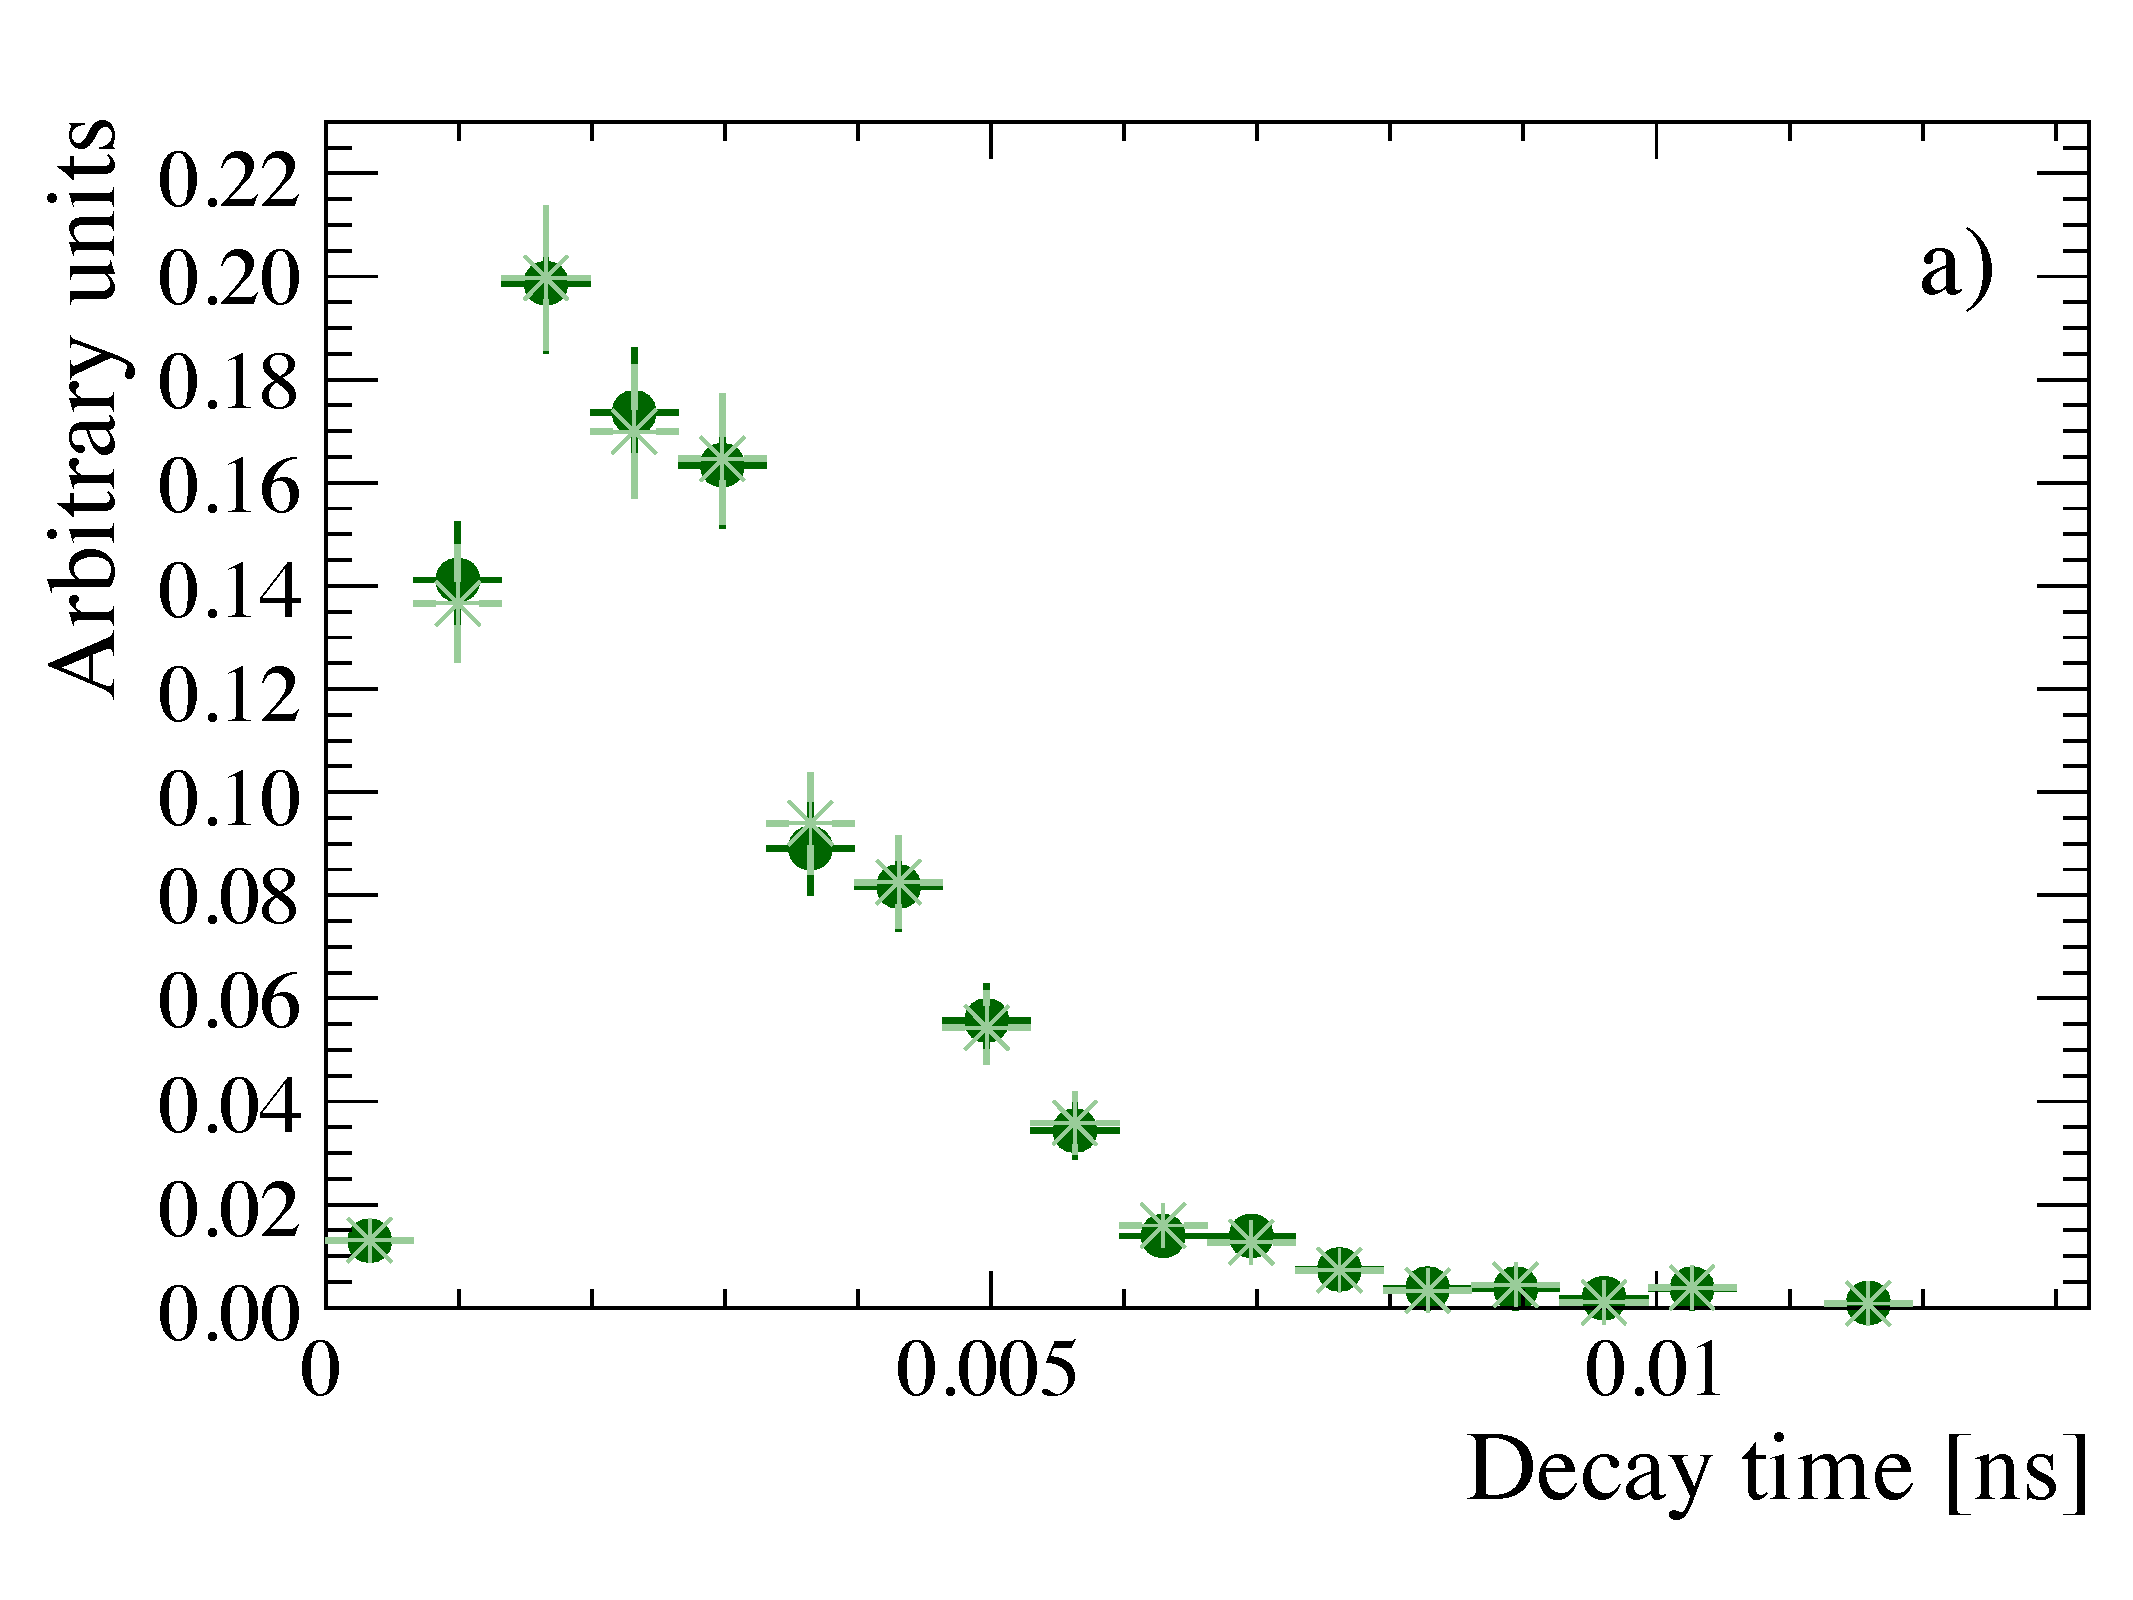
\includegraphics[width=0.49\textwidth]{./Figs/LifetimeMeasurement/2011_decaytime_Bd2KPi_weighting_impact.pdf}
    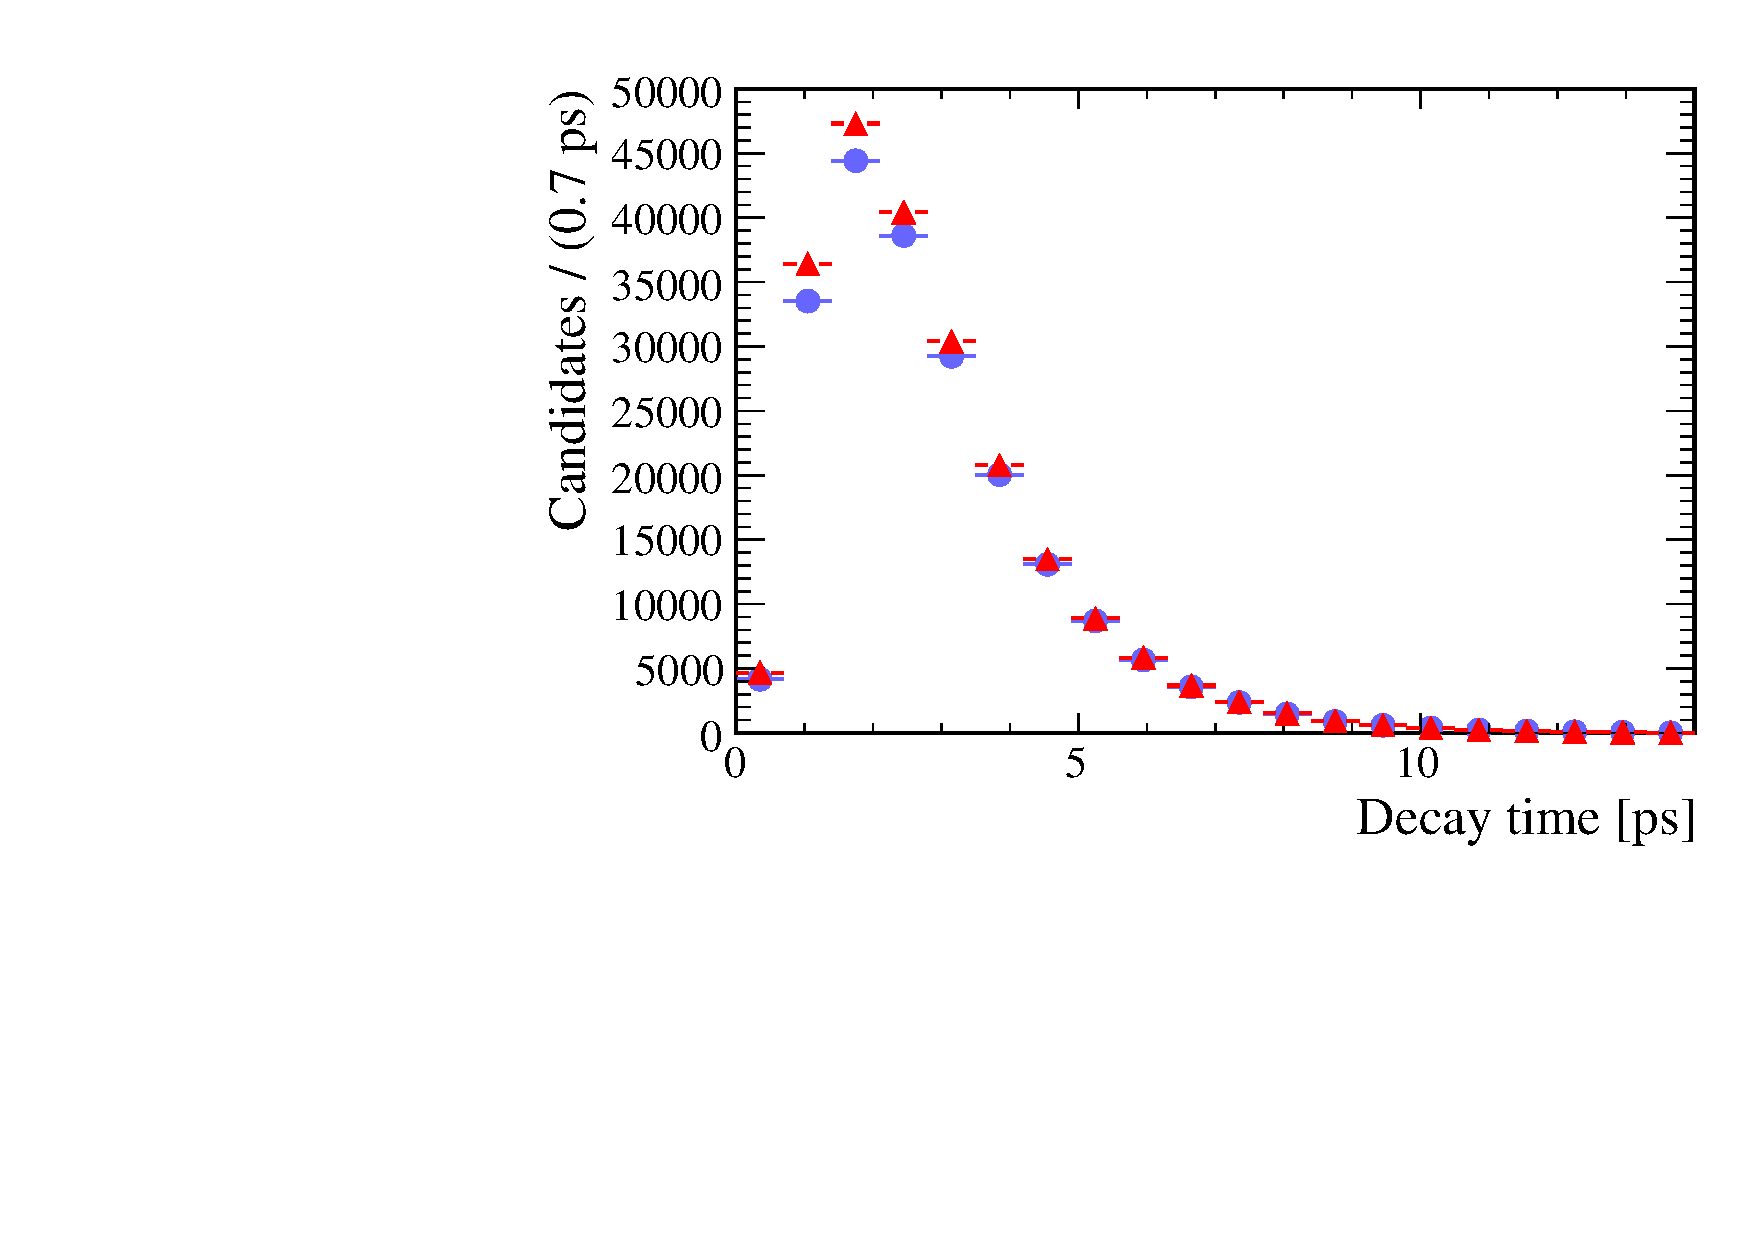
\includegraphics[width=0.49\textwidth]{./Figs/LifetimeMeasurement/2012_decaytime_Bd2KPi_weighting_impact.pdf}
    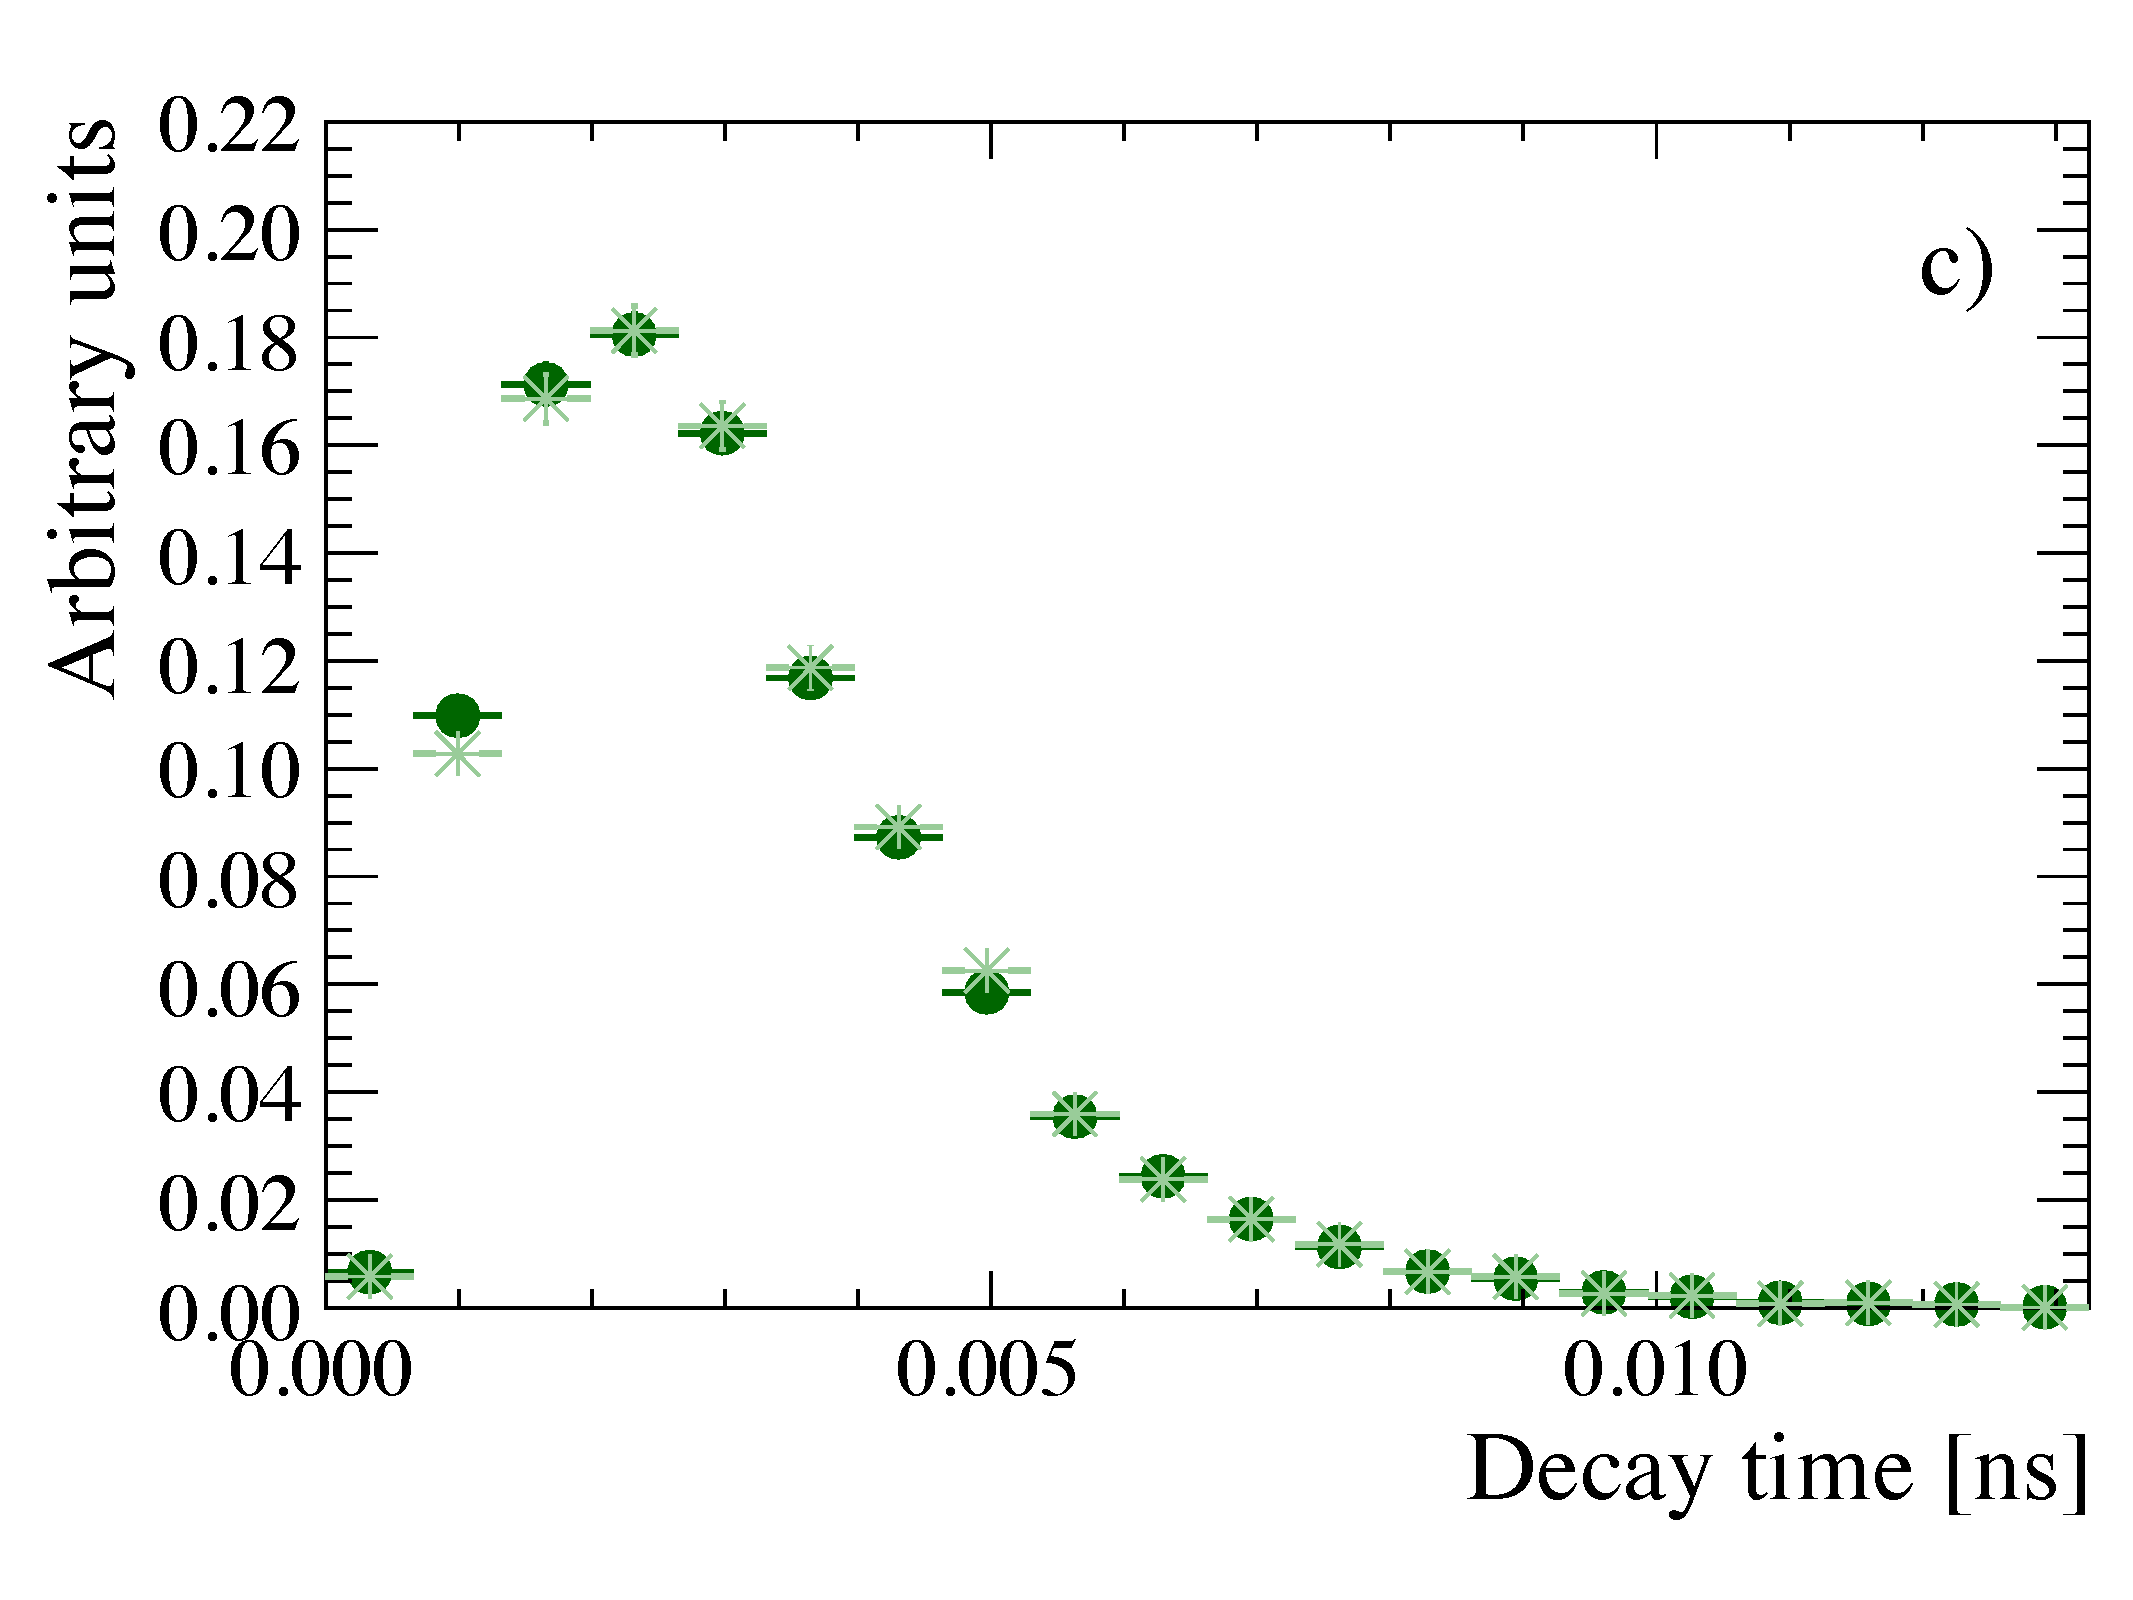
\includegraphics[width=0.49\textwidth]{./Figs/LifetimeMeasurement/2015_decaytime_Bd2KPi_weighting_impact.pdf}
    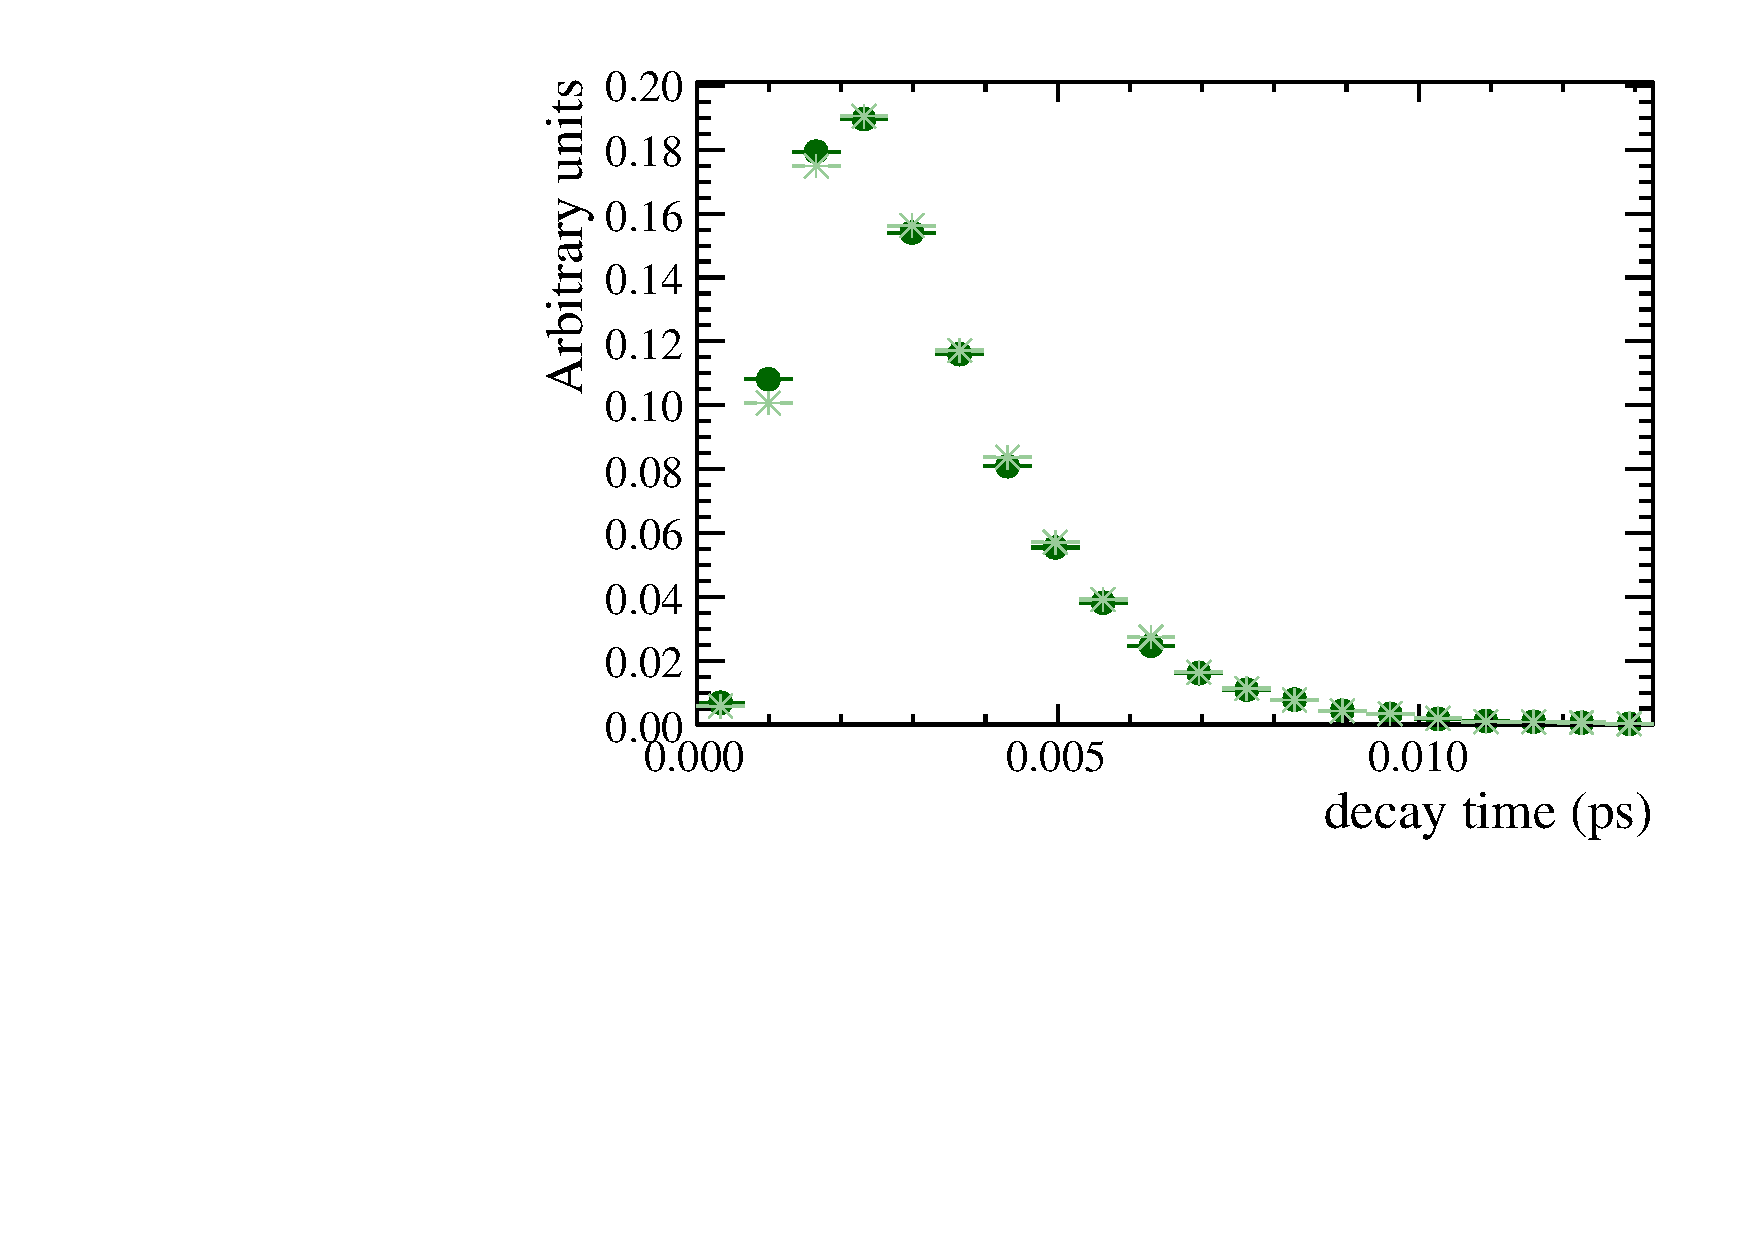
\includegraphics[width=0.49\textwidth]{./Figs/LifetimeMeasurement/2016_decaytime_Bd2KPi_weighting_impact.pdf}
  \caption{Decay time distributions for weighted and un-weighted \bdkpi simulated decays for for 2011 (top left), 2012 (top right), 2015 (bottom left) and 2016 (bottom right) data taking conditions.}
  \label{fig:BdToKpi_weightDecayTime}
\end{figure}


The same weights are applied to simulated \bsmumu decays by binning the number of tracks per event for \bsmumu decays in the same way as used for \bdkpi decays. The weights are applied to decays that pass the selection but before the global BDT cut is applied. The change in the decay time distribution before and after reweighting for \bsmuu simulated decays after the global BDT cut is shown in Figure~\ref{fig:BsmmDT}. %in the comparison of weighted and un-weighted \bsmumu decay time distributions. 
Similar to \bdkpi decays the largest effect is at low decay times where the change in selection efficiency is greatest as seen in Figure~\ref{fig:accpteg}.

The reweighting relies on the number of tracks per event being very similar for \bdkpi and \bsmumu decays. This cannot be evaluated in data due to the small number of \bsmumu decays in data. However, Figure~\ref{fig:BsmmVsBdToKpinTracks} shows a comparison of the number of tracks per event for simulated \bsmumu and \bdkpi decays in each year and resulting distributions are rather similar.



\begin{figure}[tbp]
  \centering
    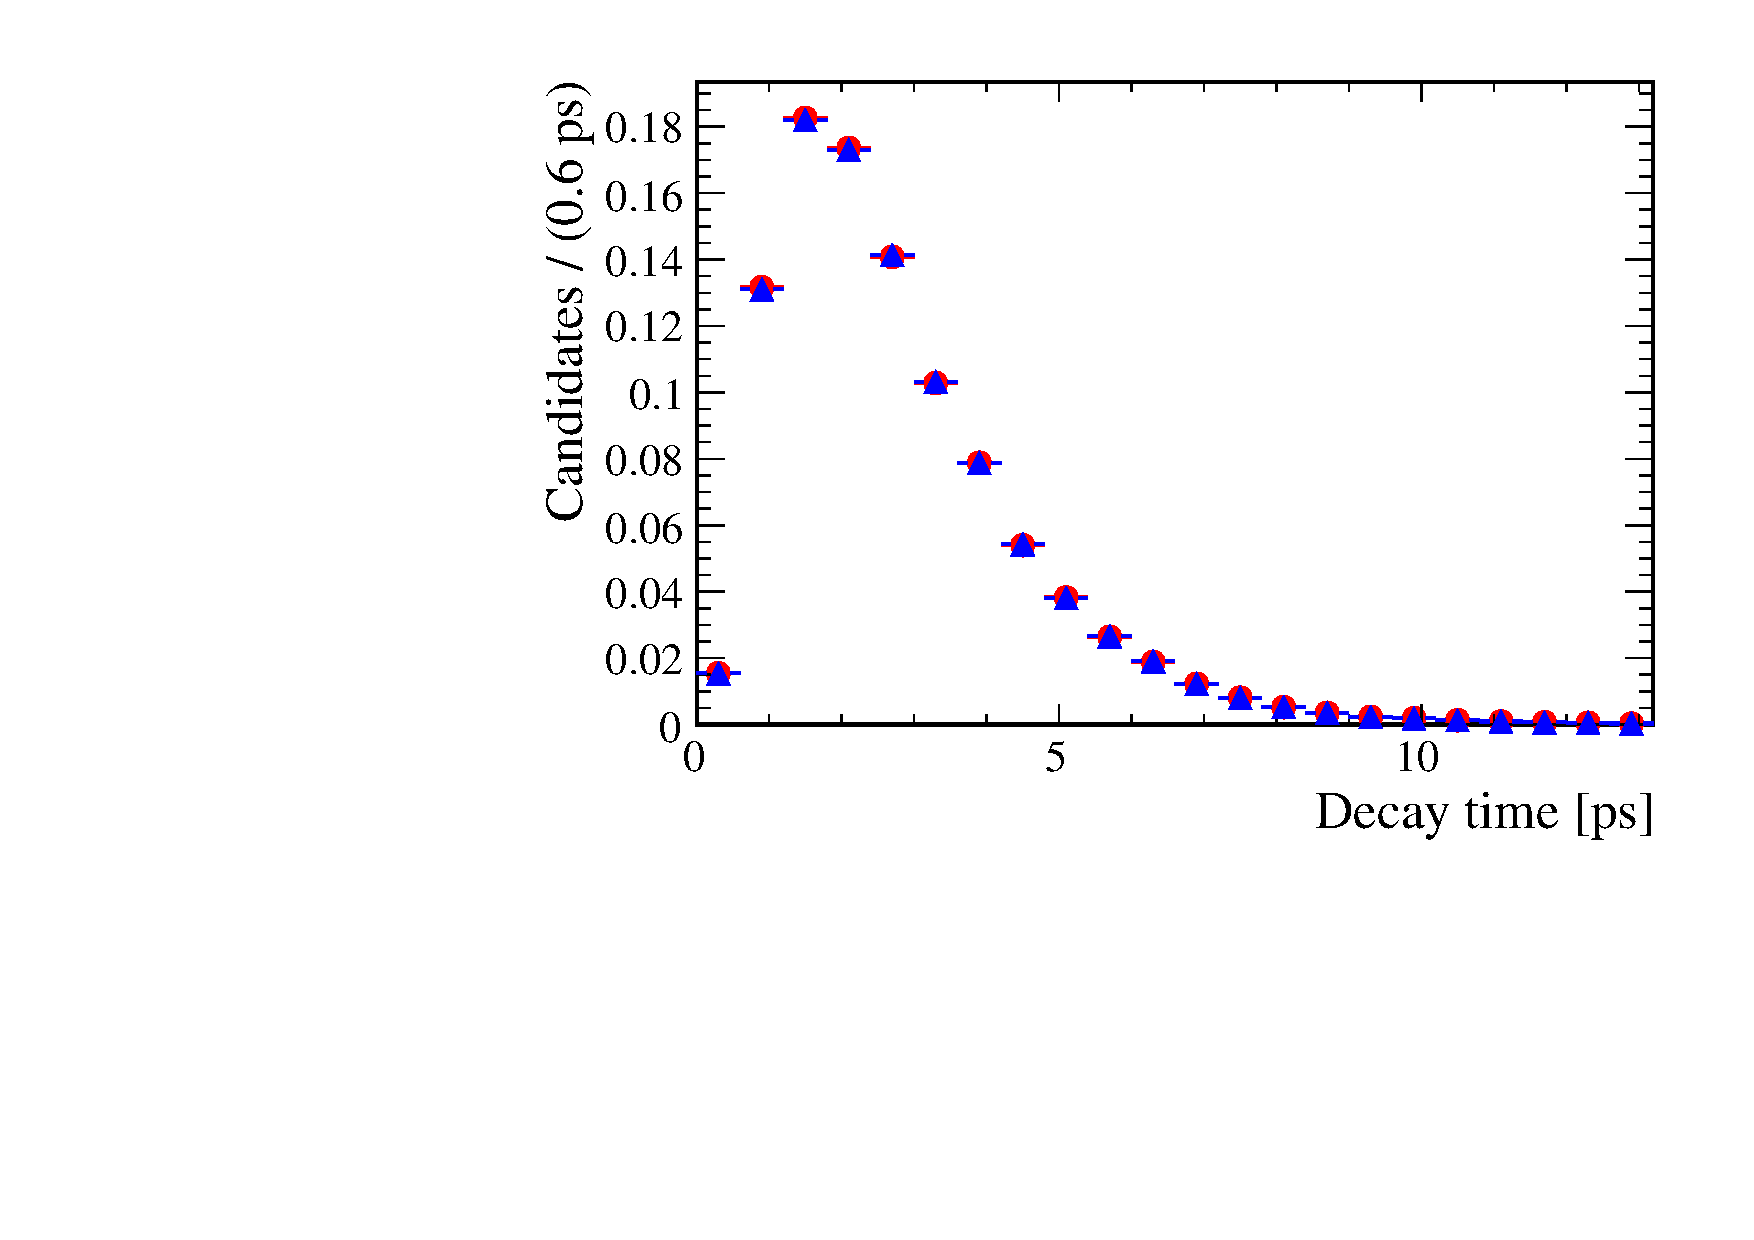
\includegraphics[width=0.49\textwidth]{./Figs/LifetimeMeasurement/2011_DT_Bs2MuMu.pdf}
    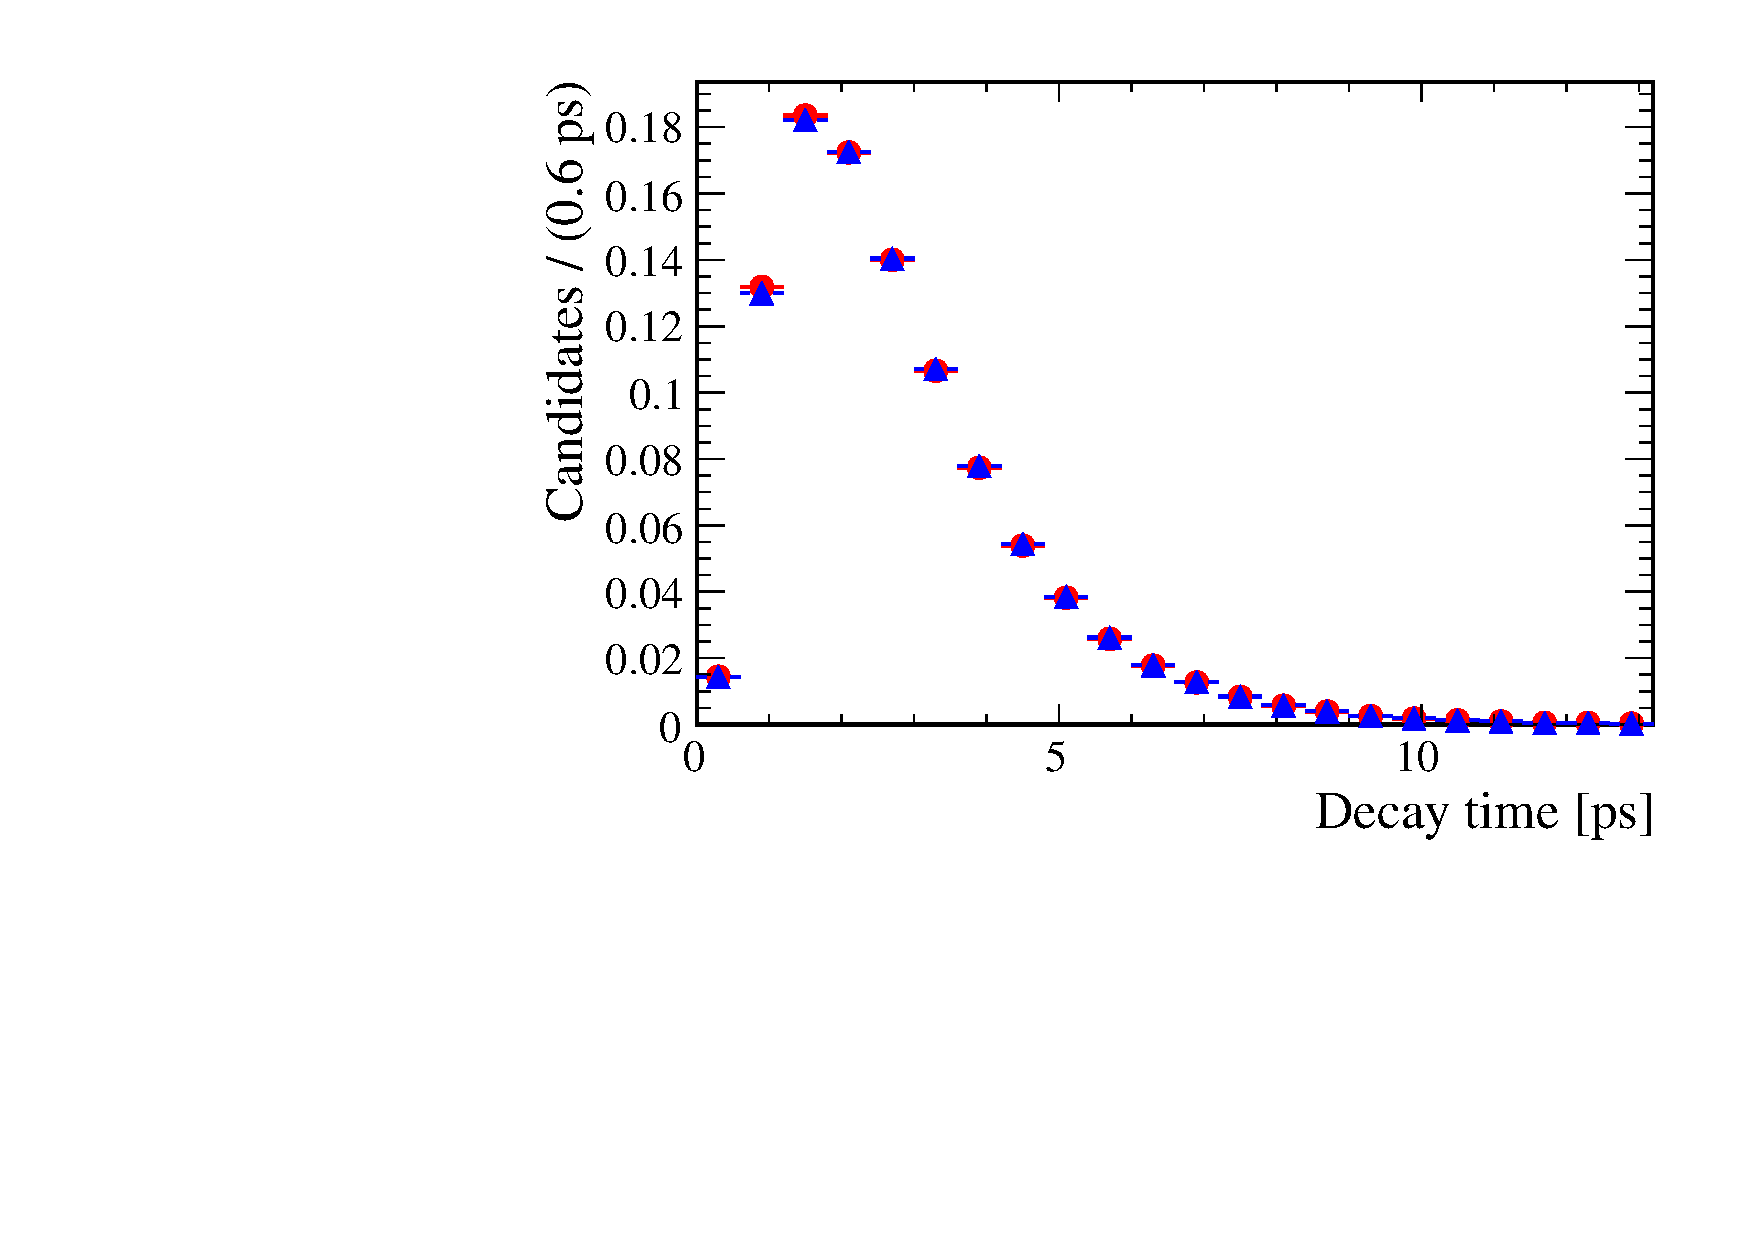
\includegraphics[width=0.49\textwidth]{./Figs/LifetimeMeasurement/2012_DT_Bs2MuMu.pdf}
    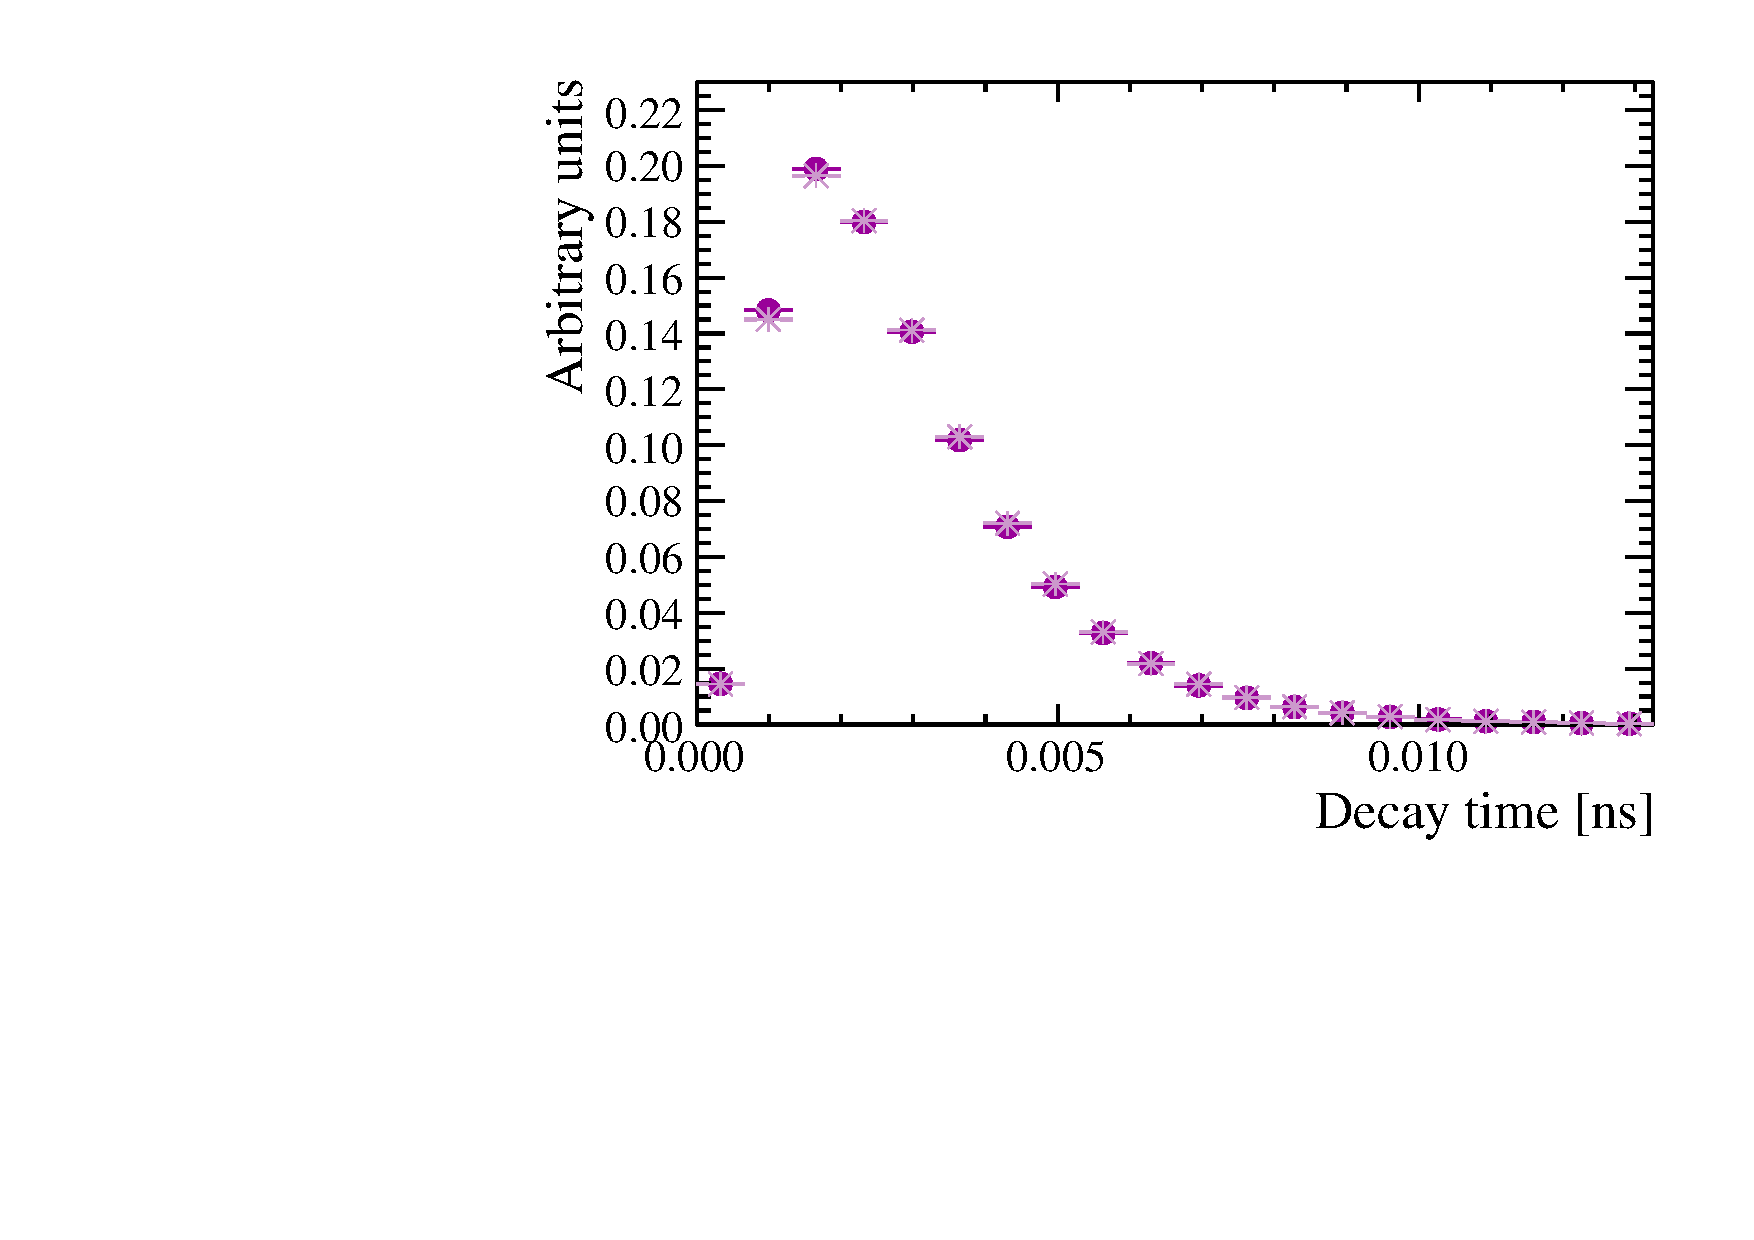
\includegraphics[width=0.49\textwidth]{./Figs/LifetimeMeasurement/2015_DT_Bs2MuMu.pdf}
    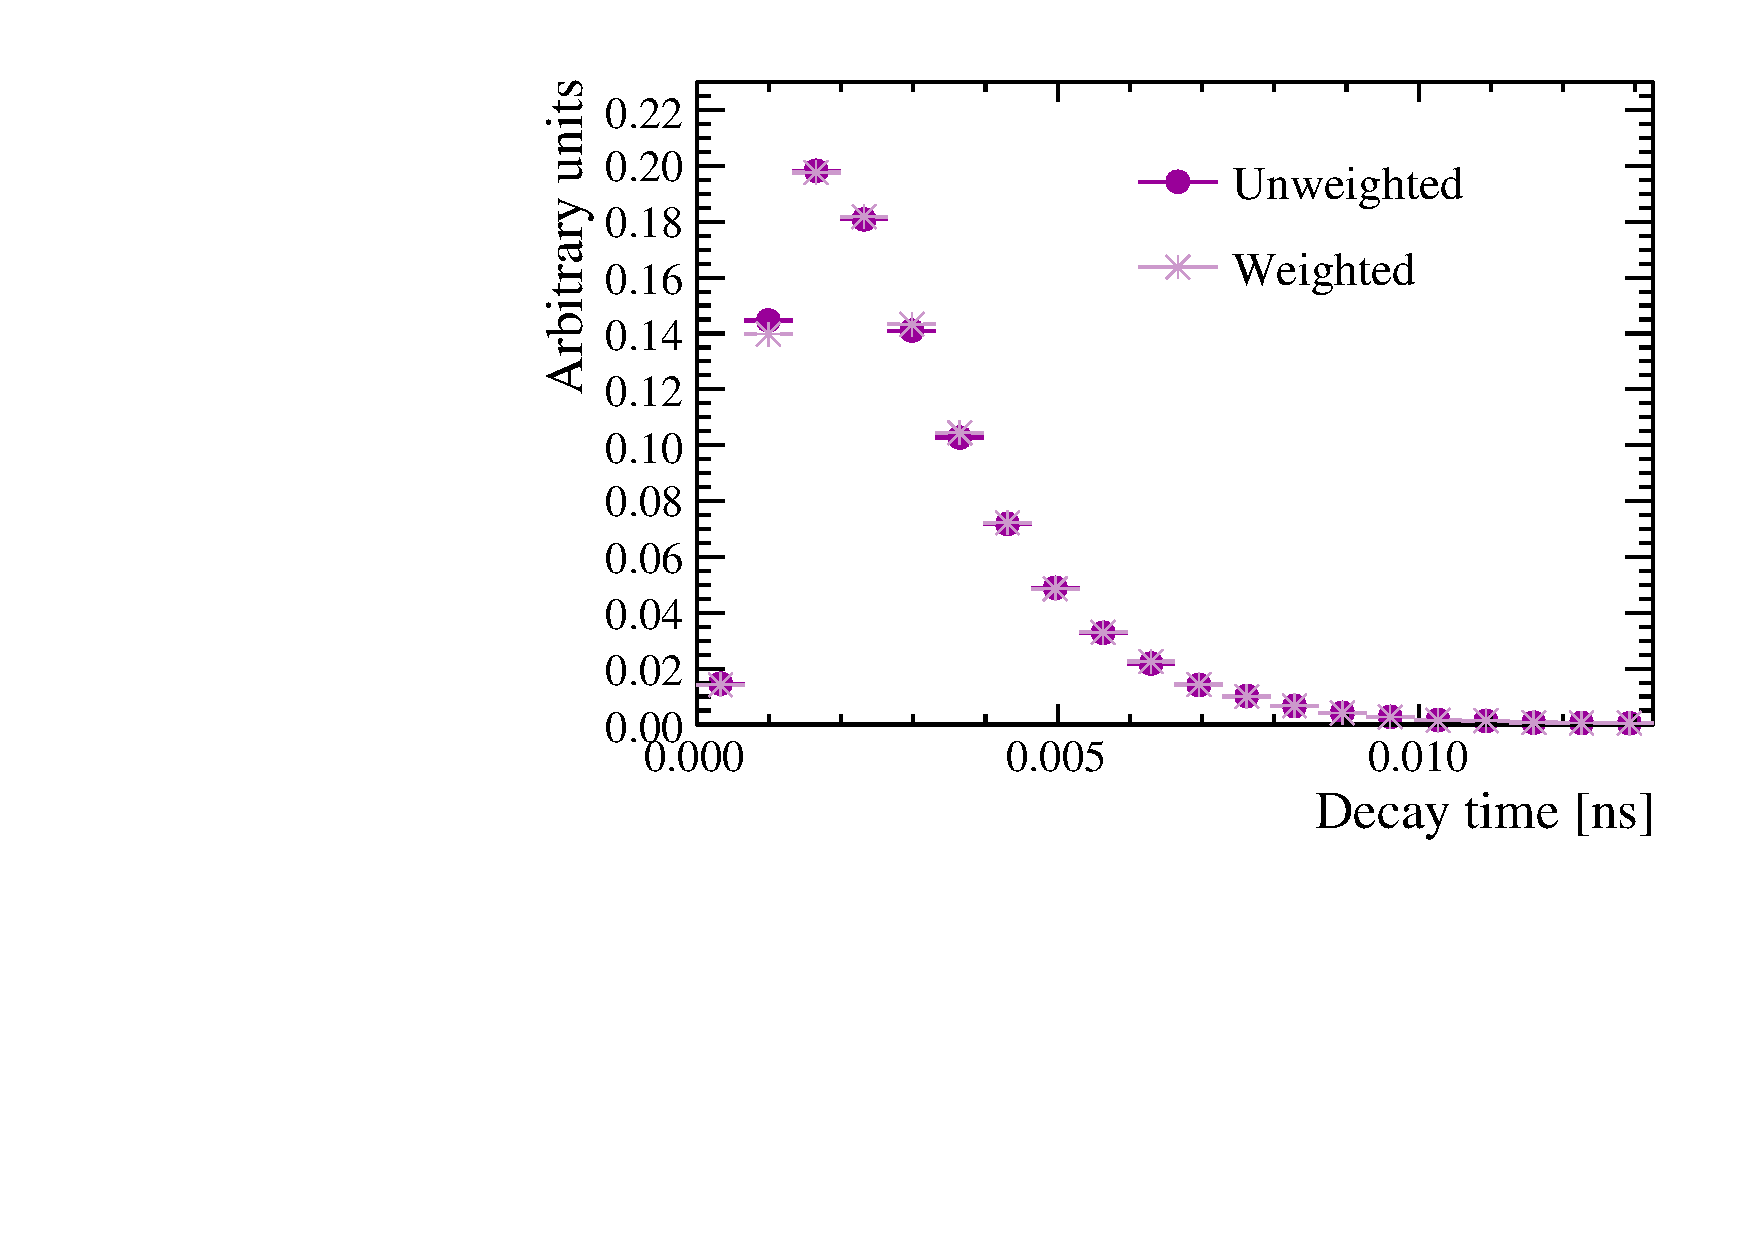
\includegraphics[width=0.49\textwidth]{./Figs/LifetimeMeasurement/2016_DT_Bs2MuMu.pdf}
  \caption{Decay time distributions for weighted (blue) and un-weighted (red) \bsmumu simulated decays for for 2011 (top left), 2012 (top right), 2015 (bottom left) and 2016 (bottom right) data taking conditions. Distributions have been normalised to have unit area.}
  \label{fig:BsmmDT}
\end{figure}

\begin{figure}[tbp]
  \centering
    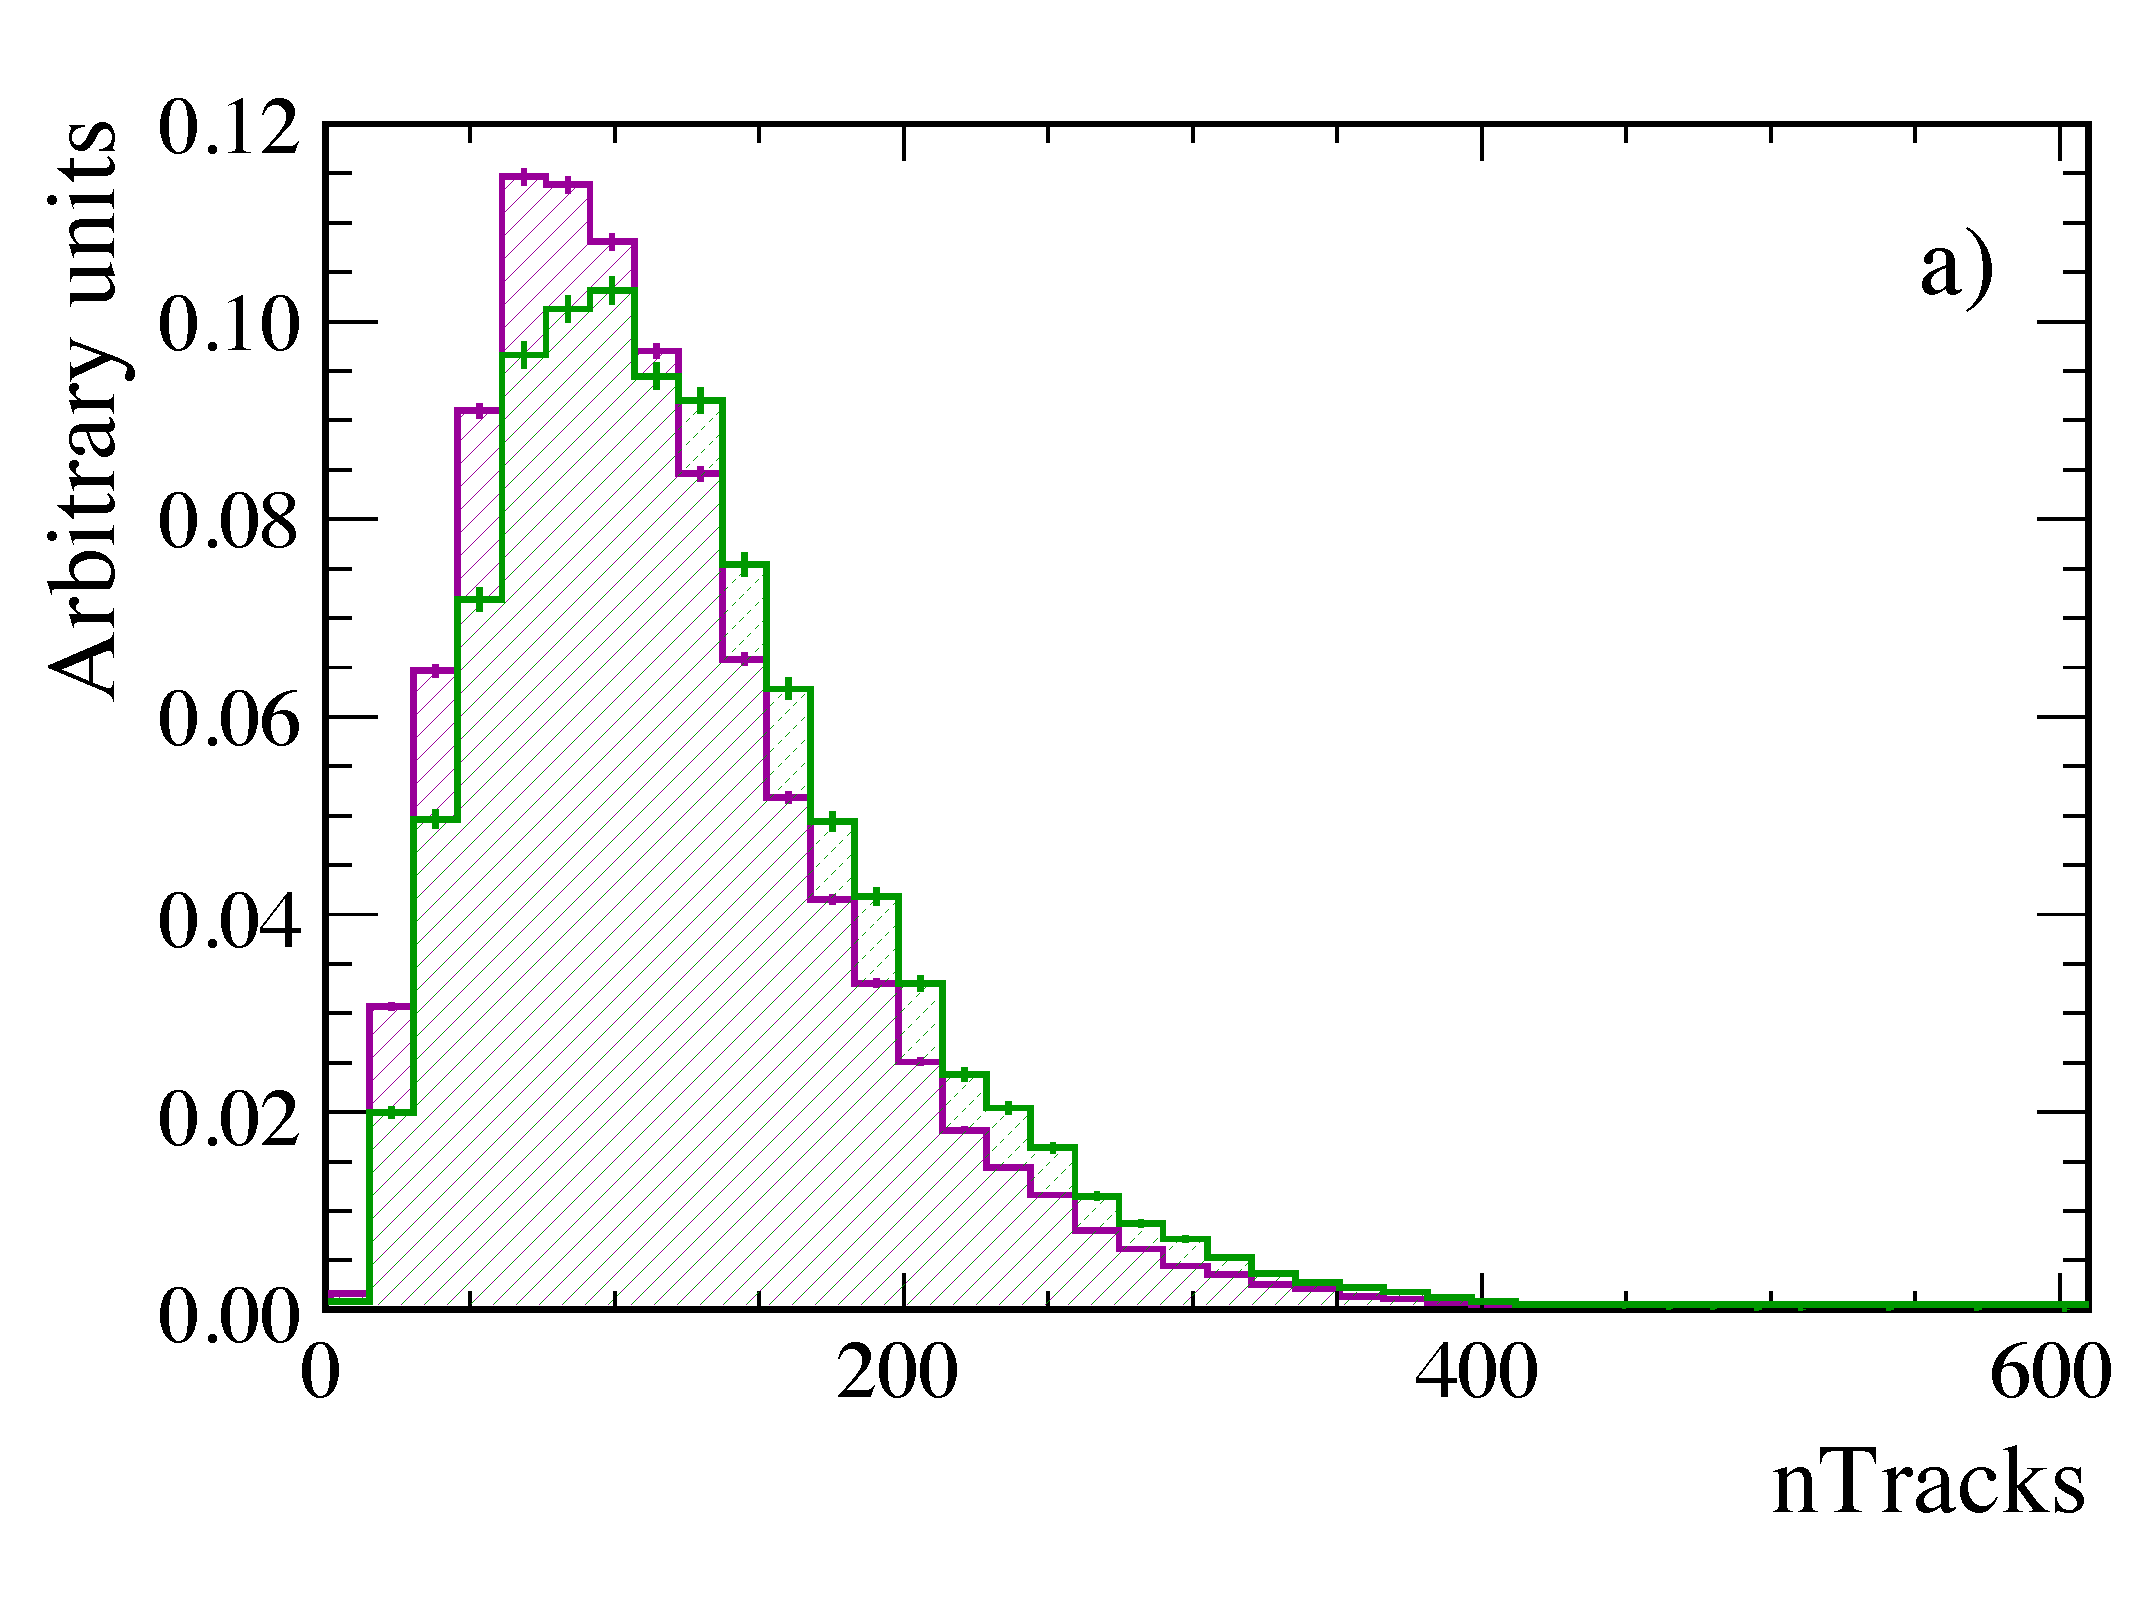
\includegraphics[width=0.49\textwidth]{./Figs/LifetimeMeasurement/nTracks_2011_Bs2MuMu_Bd2KPi.pdf}
    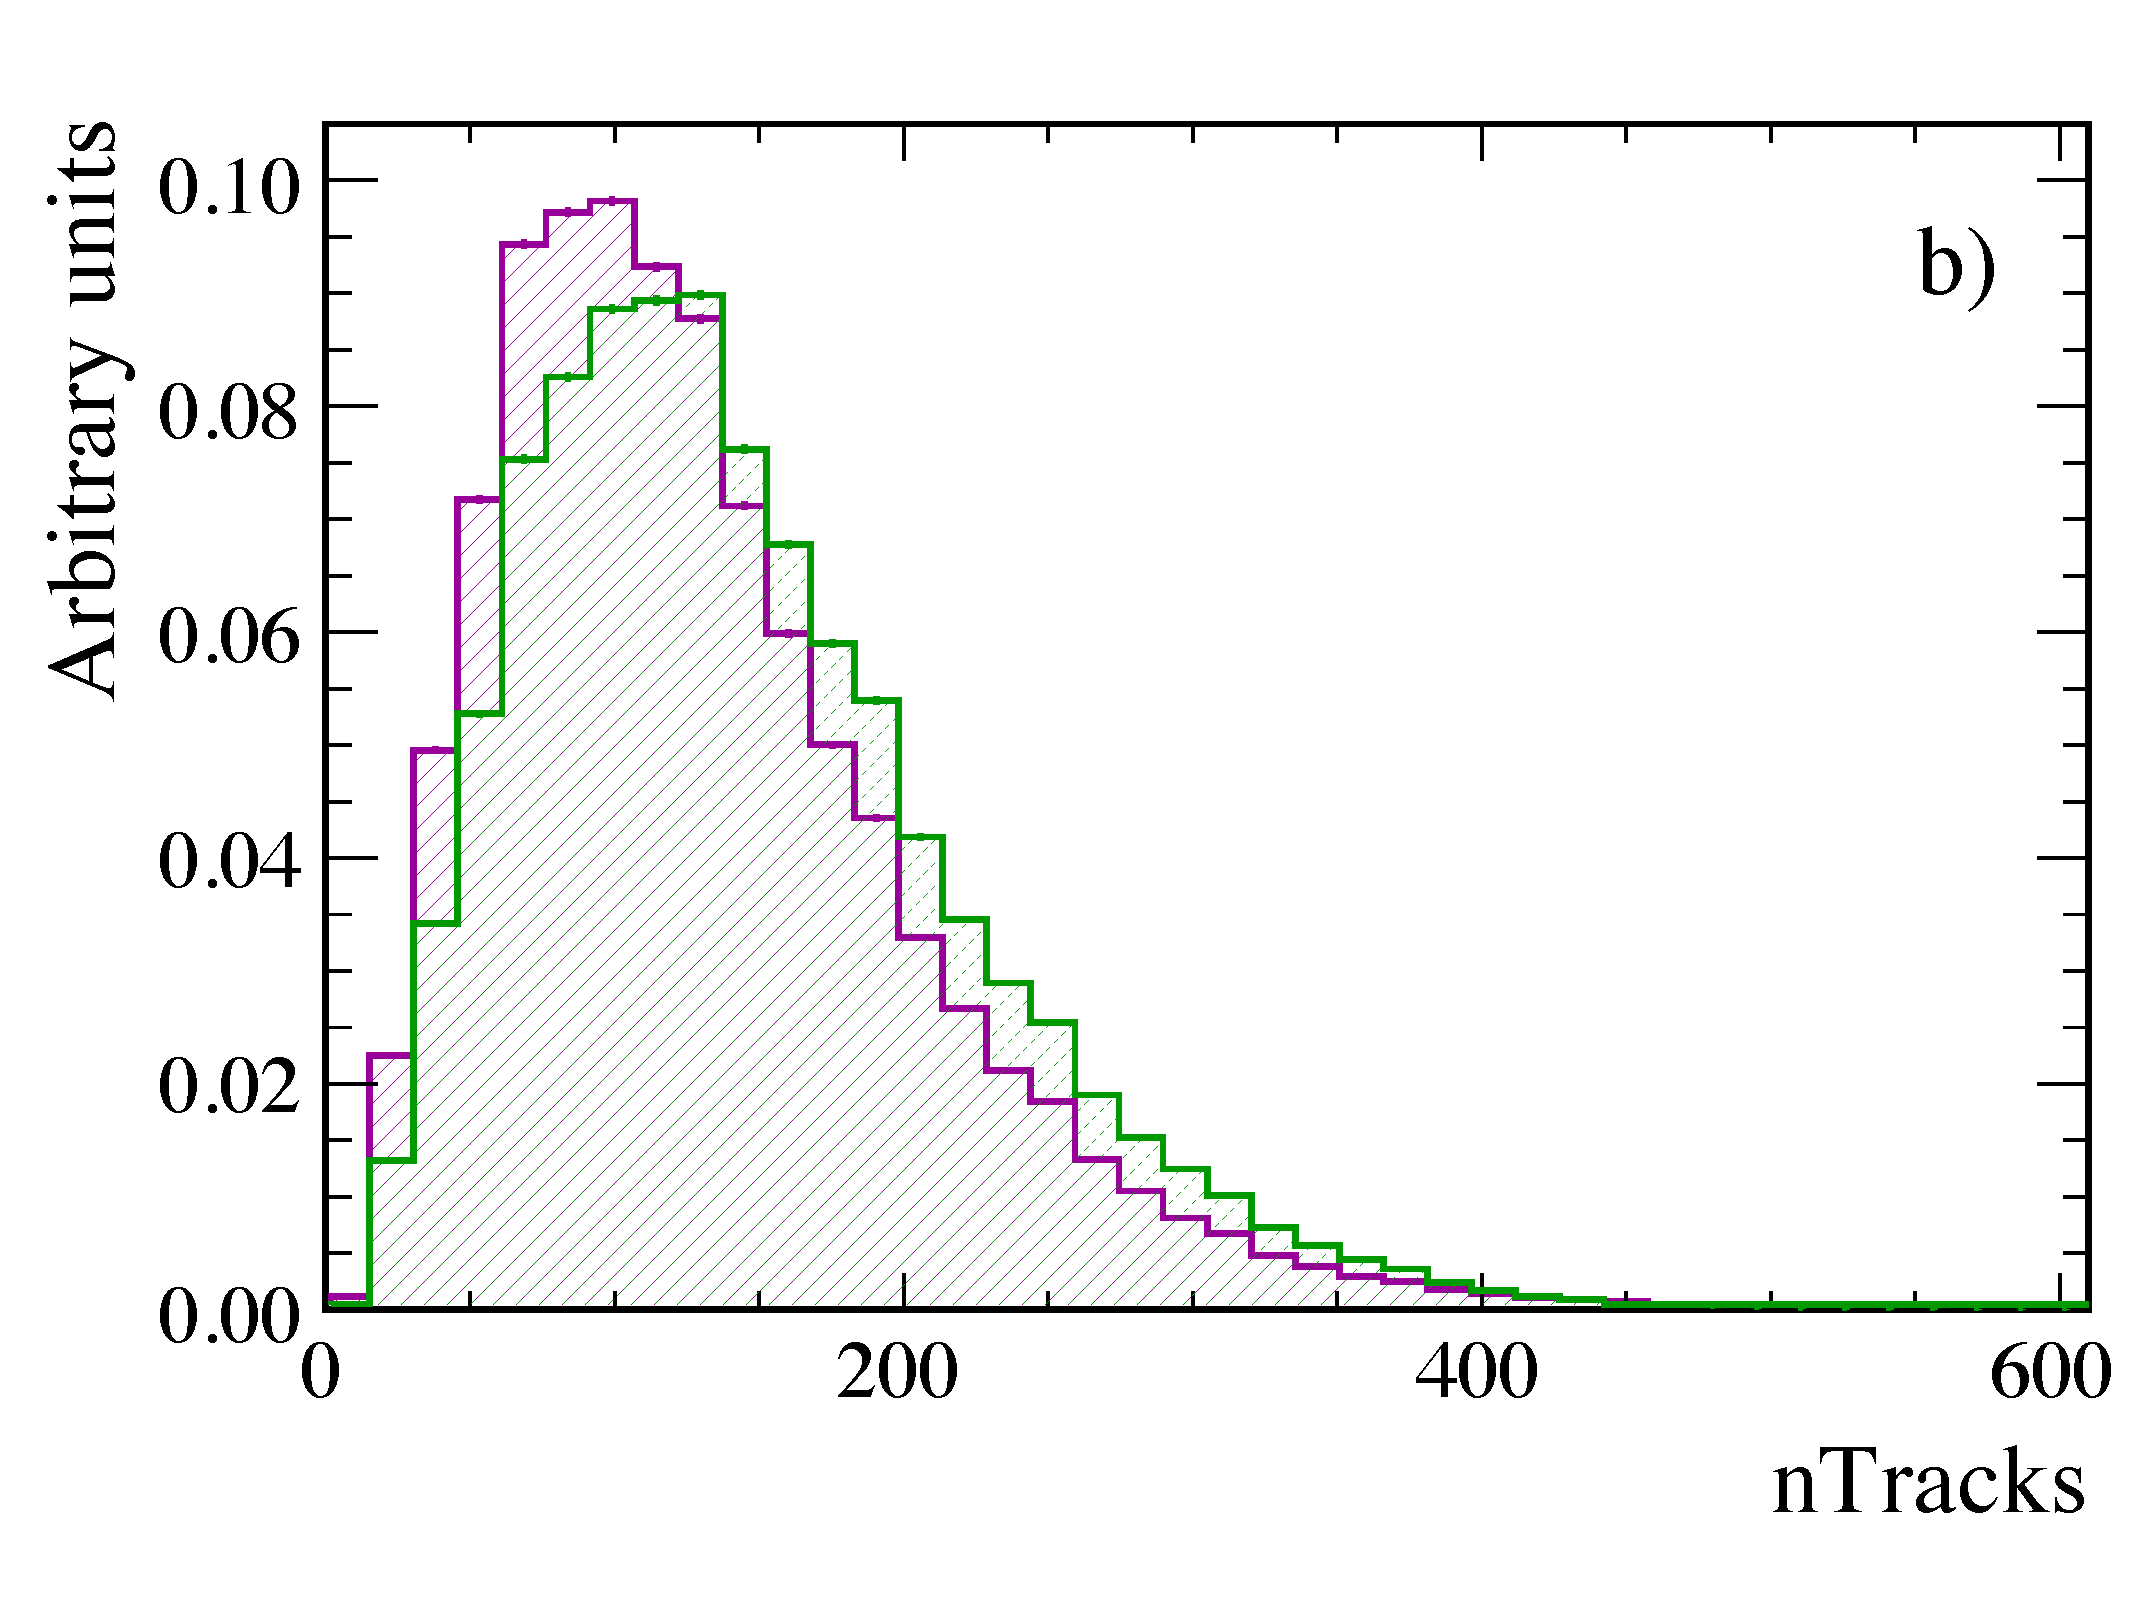
\includegraphics[width=0.49\textwidth]{./Figs/LifetimeMeasurement/nTracks_2012_Bs2MuMu_Bd2KPi.pdf}
    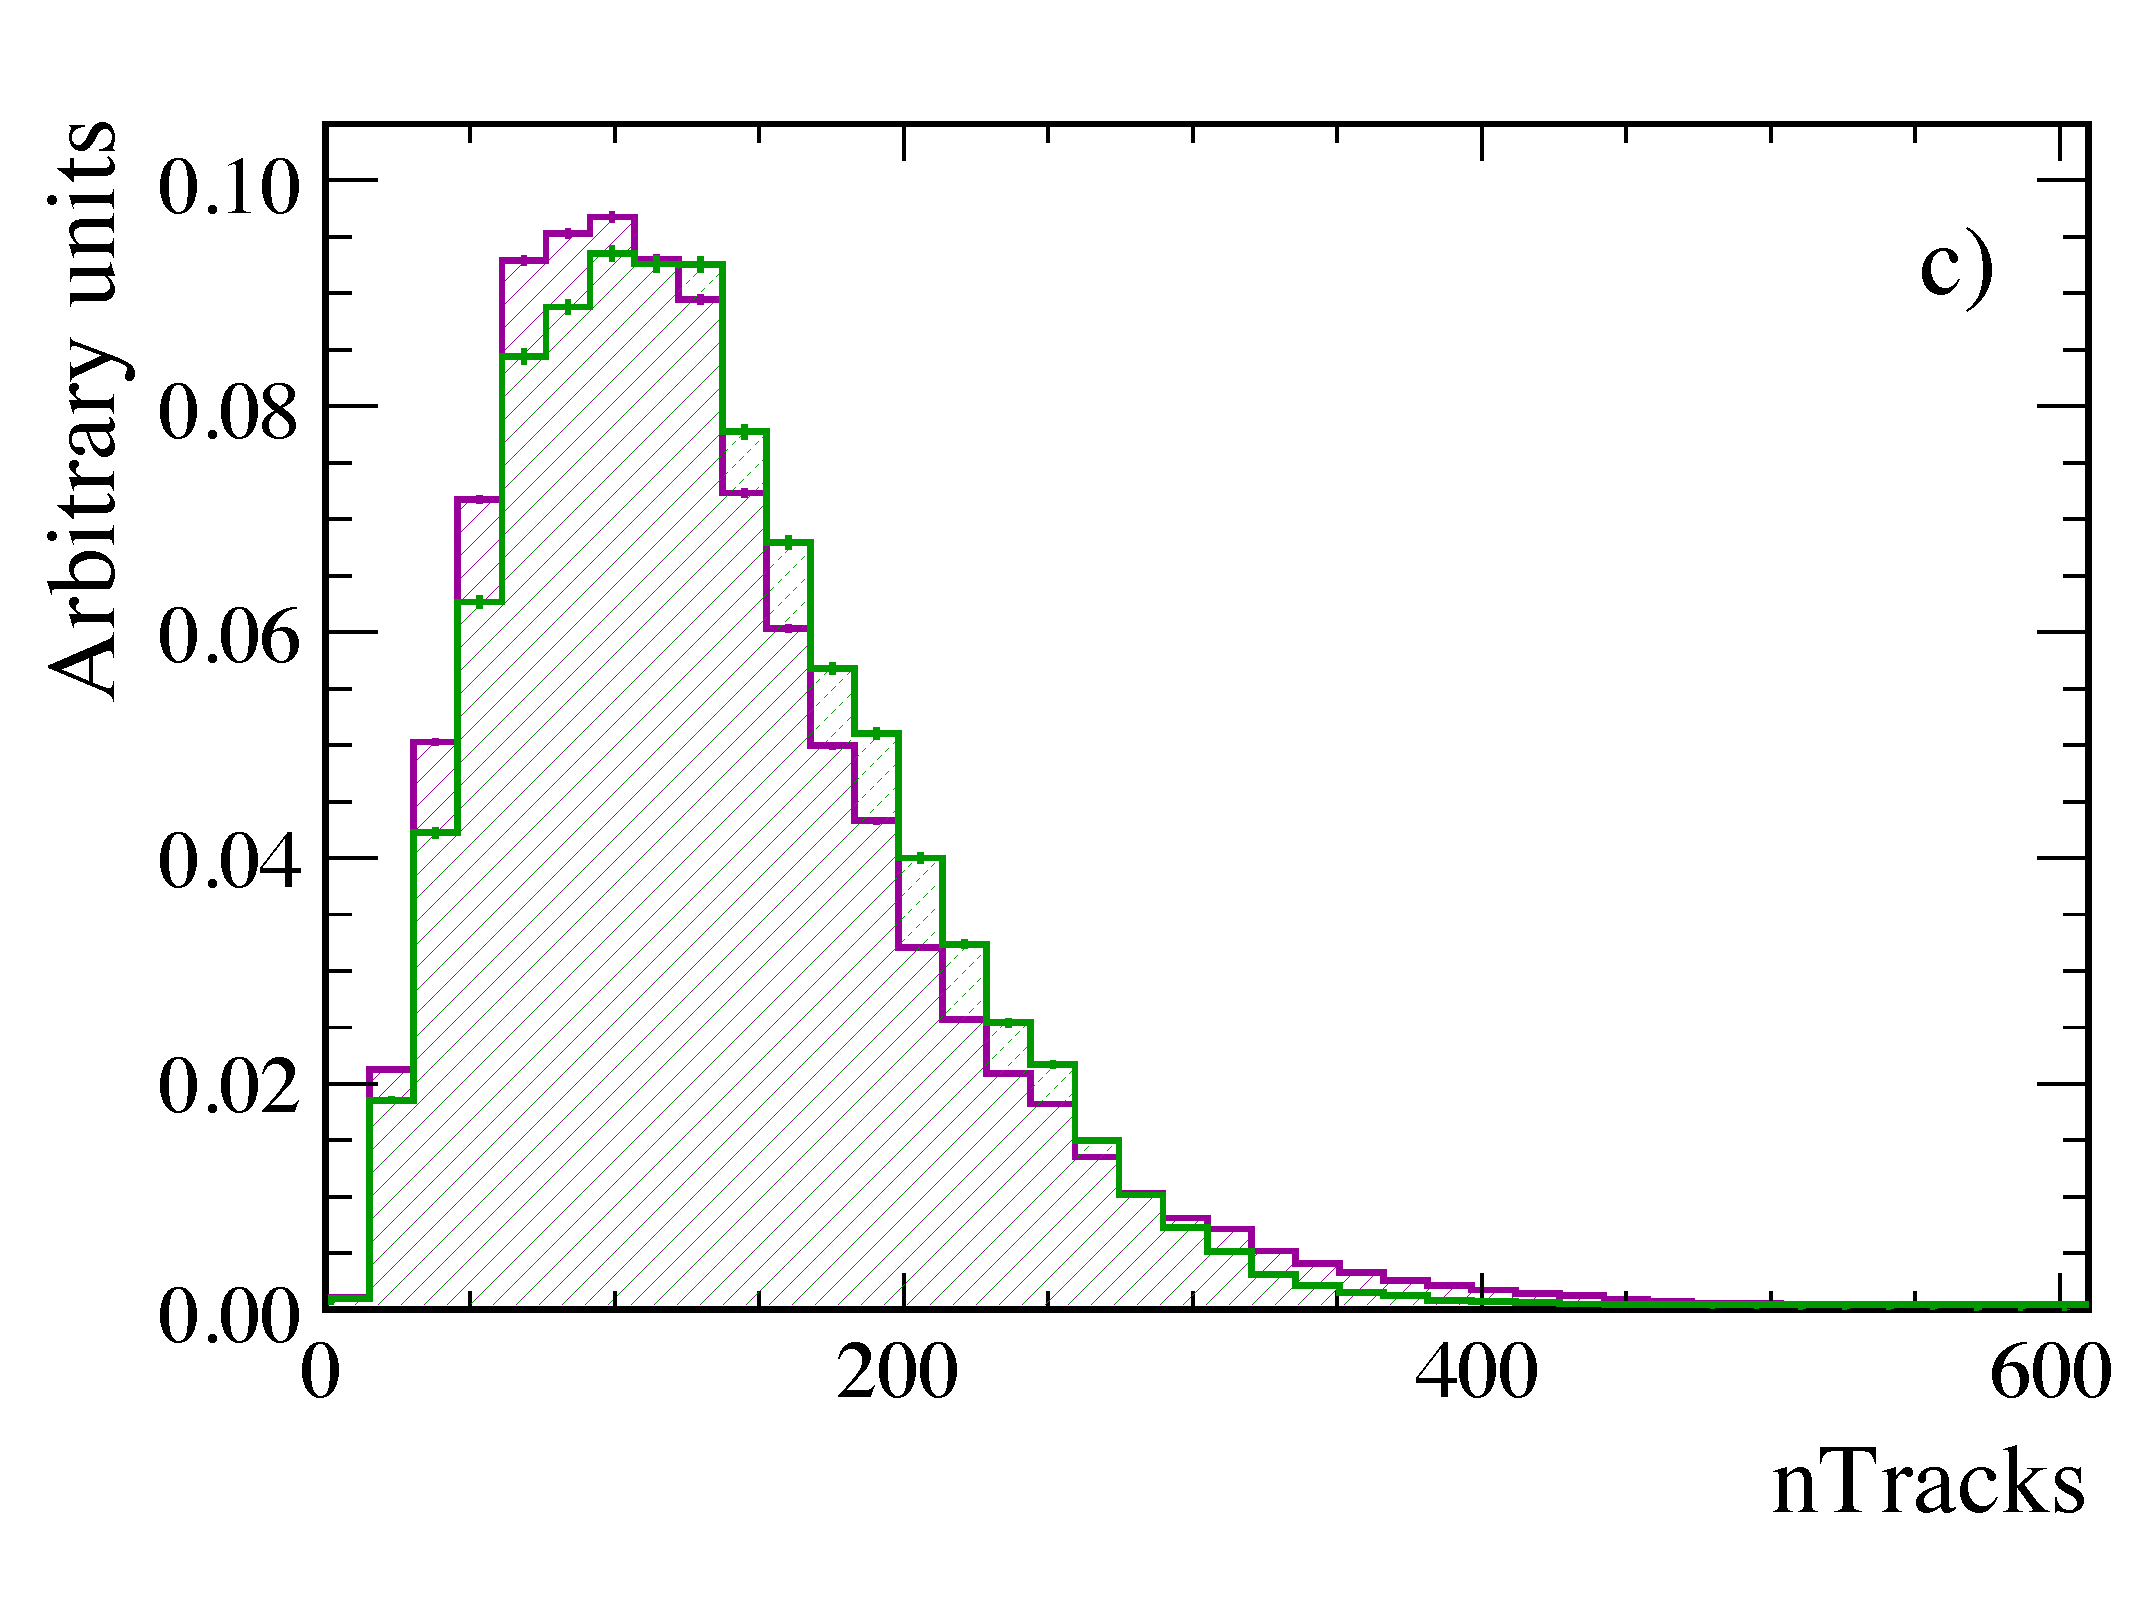
\includegraphics[width=0.49\textwidth]{./Figs/LifetimeMeasurement/nTracks_2015_Bs2MuMu_Bd2KPi.pdf}
    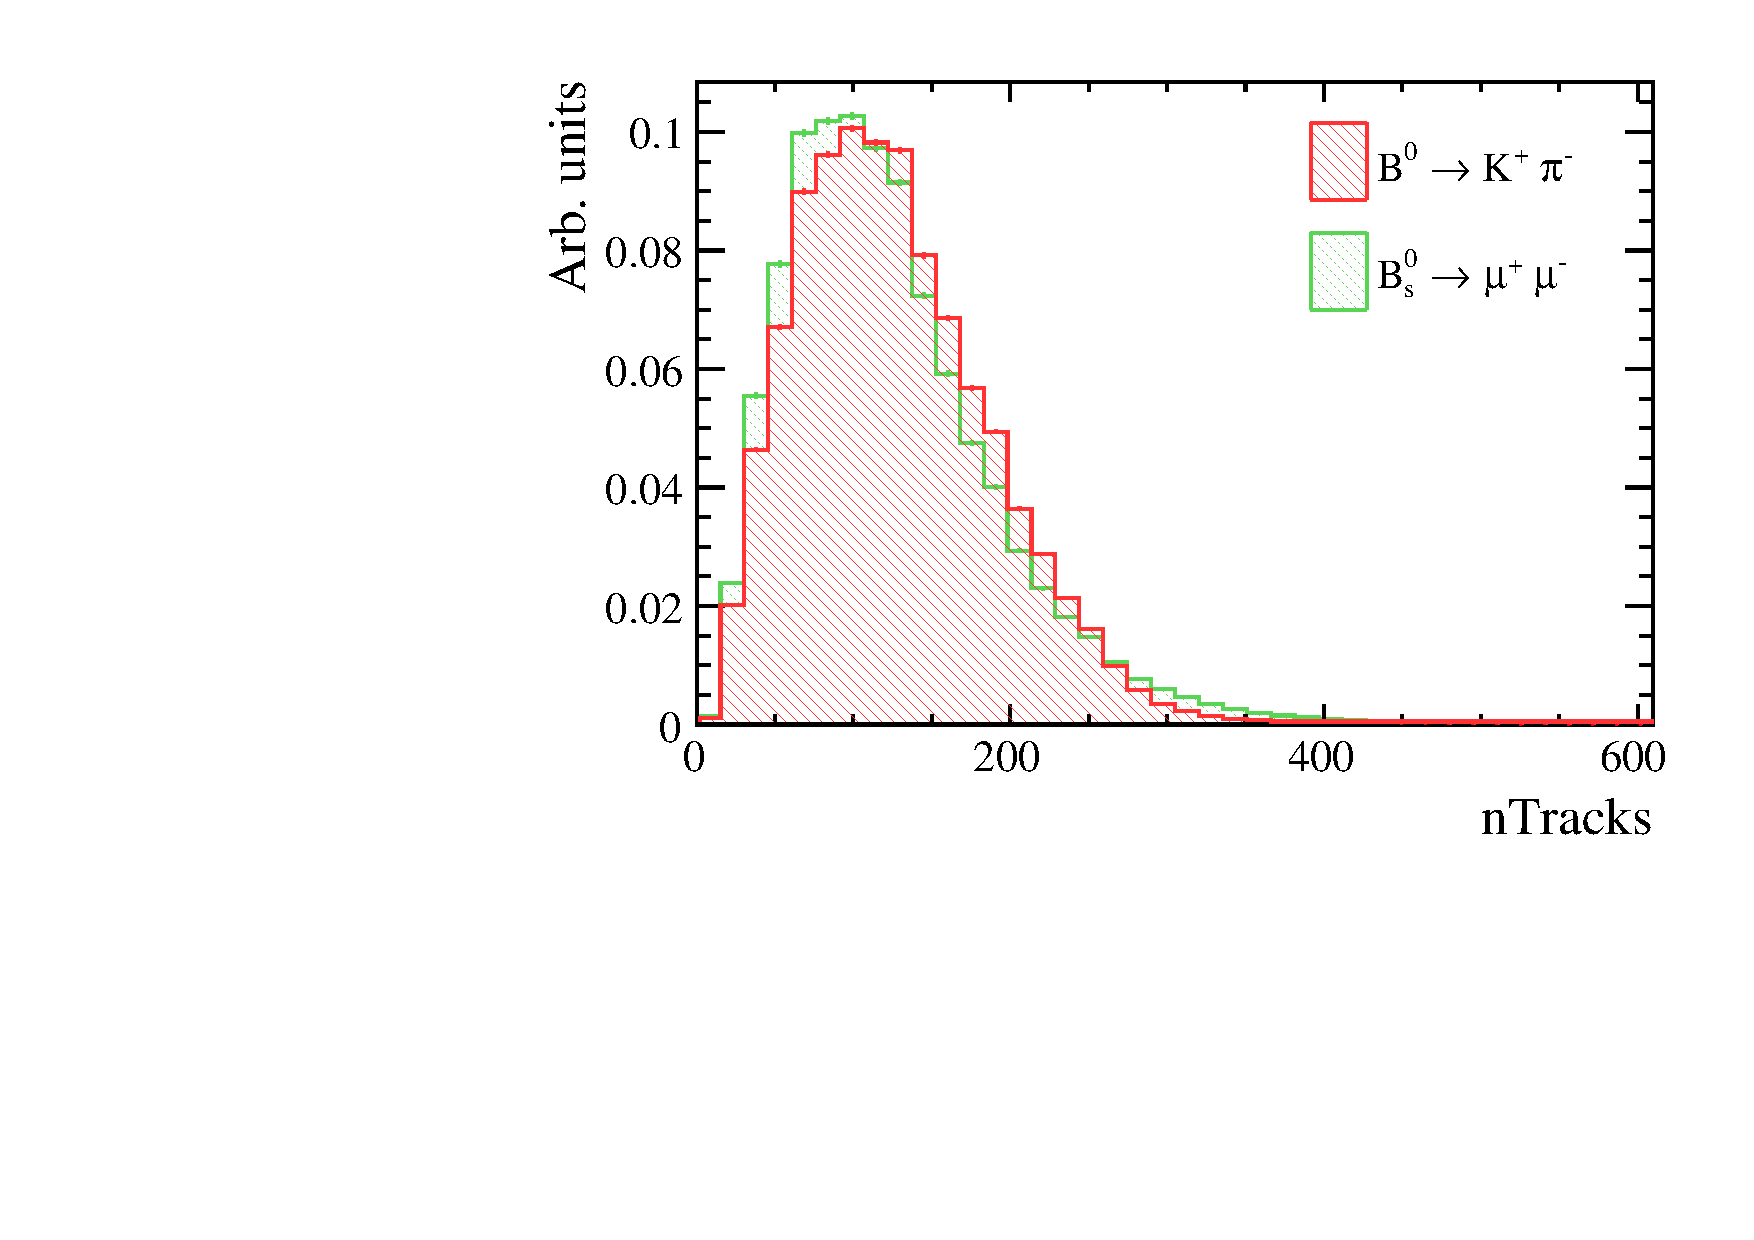
\includegraphics[width=0.49\textwidth]{./Figs/LifetimeMeasurement/nTracks_2016_Bs2MuMu_Bd2KPi.pdf}
  \caption{Normalised histograms of the number of tracks per event in simulated \bdkpi and \bsmumu decays in data for 2011 (top left), 2012 (top right), 2015 (bottom left) and 2016 (bottom right) data. }
  \label{fig:BsmmVsBdToKpinTracks}
\end{figure}
%accptance from MC problems can in Bd2kPi decays - was is just Run 2 or both? Could the problem actually have been sim09a not MC in general?

The decay time efficiency will now be accurately modelled in the weighted simulated \bsmumu decays and the parameters in the acceptance function can be evaluated. Each year of data taking is treated separately due to the different \bs lifetimes used in the simulation generation, selection and trigger efficiencies. The number of simulated decays available for each year does not correspond to the proportions of decays present in each year of the data. Therefore, weights are used to combine the simulated decays so that the combined set of decays has the same proportions of decays for each year as the complete data set. 
The proportion of events in each year is taken from the number of \bsjpsiphi decays in data for each year corrected for the selection differences for \bsmumu and \bsjpsiphi decays. The \bsjpsiphi yields, $Y^{J/\psi \phi}$, are extracted from maximum likelihood fits to the mass spectrum of candidates in each year of data taking. The selection applied to identify \bsjpisphi candidates is very similar to that applied to \bsmumu decays apart from the particle identification and global BDT requirements. This decay is chosen because the ratio of the efficiencies for the stripping, trigger and pre-selection requirements of \bsmumu and \bsjpsiphi decays is uniform across the different years making \bsjpsiphi decays a good proxy for \bsmumu. 
The weights applied to simulated \bsmumu decays are
\begin{equation}
\omega_{i}  = \frac{Y_{i}^{J/\psi \phi} \epsilon_{i}}{\displaystyle\sum_{j} Y_{j}^{J/\psi \phi} \epsilon_{j}} \cdot \frac{\displaystyle\sum_{k} N_{k}^{\mu^{+}\mu^{-}}}{N_{i}^{\mu^{+}\mu^{-}}},
\end{equation}
where $i$ represents the year and $N^{\mu^{+}\mu^{-}_{i}$ the number of simulated \bsmumu decays available for the year passing the full \bsmumu selection and $\epsilon_{i}$ the efficiency of the particle identification and global BDT requirements for \bsmumu decays that have passed all other selection requirement evaluated from simulated decays. The sums, over $k$ and $j$, are performed over all years of data taking. The weights applied to simulated \bsmumu decays and values of the different components of the weights are given in Table~\ref{tab:MCWeightInfo}.

\begin{table}[ht]
\begin{center}
\begin{tabular}{lccccc}
\toprule \toprule
Year ($i$) & $Y_i^{\JPsiPhi}$ & $\epsilon_i$ & $N^{\mumu}_i$ & $\omega_i$ & $\mathcal{N}^{\mumu}_i \equiv N^{\mumu}_i \omega_i$ \\ \midrule 
2011       & 19190           & 0.412        & 70448        & 1.72       & 131364 \\
2012       & 42103           & 0.406        & 254822       & 1.03       & 262461 \\
2015       & 8571            & 0.410        & 222820       & 0.24       & 53917 \\ 
2016       & 37765           & 0.406        & 124870       & 1.88       & 235218 \\ \bottomrule \bottomrule
\end{tabular}
\vspace{0.7cm}                                                                                                                                               
\caption{Weights used to combine simulated \bsmumu decays for each year to determine the acceptance function. Weights ensure the proportion of simulated events for each year matches what is expected in data.}
\label{tab:MCWeightInfo}
\end{center}
\vspace{-1.0cm}                                                                                                                                               
\end{table}
An unbinned \ml fit is performed to the combined simulated \bsmumu decays to determine the acceptance parameters in Equation~\ref{eq:accpt}. In the fit the acceptance parameters are free and the \bsmumu lifetime is constrained to the weighted average of lifetimes used to generate each year of simulated decays. The fit results are shown in Figure~\ref{fig:accptfit} and the acceptance parameters are given in Table~\ref{tab:accptsig}. Figure~\ref{fig:accptplot} shows the selection efficiency histogram as a function of decay time with the acceptance function overlaid.




\begin{figure}[tbp]
    \centering
        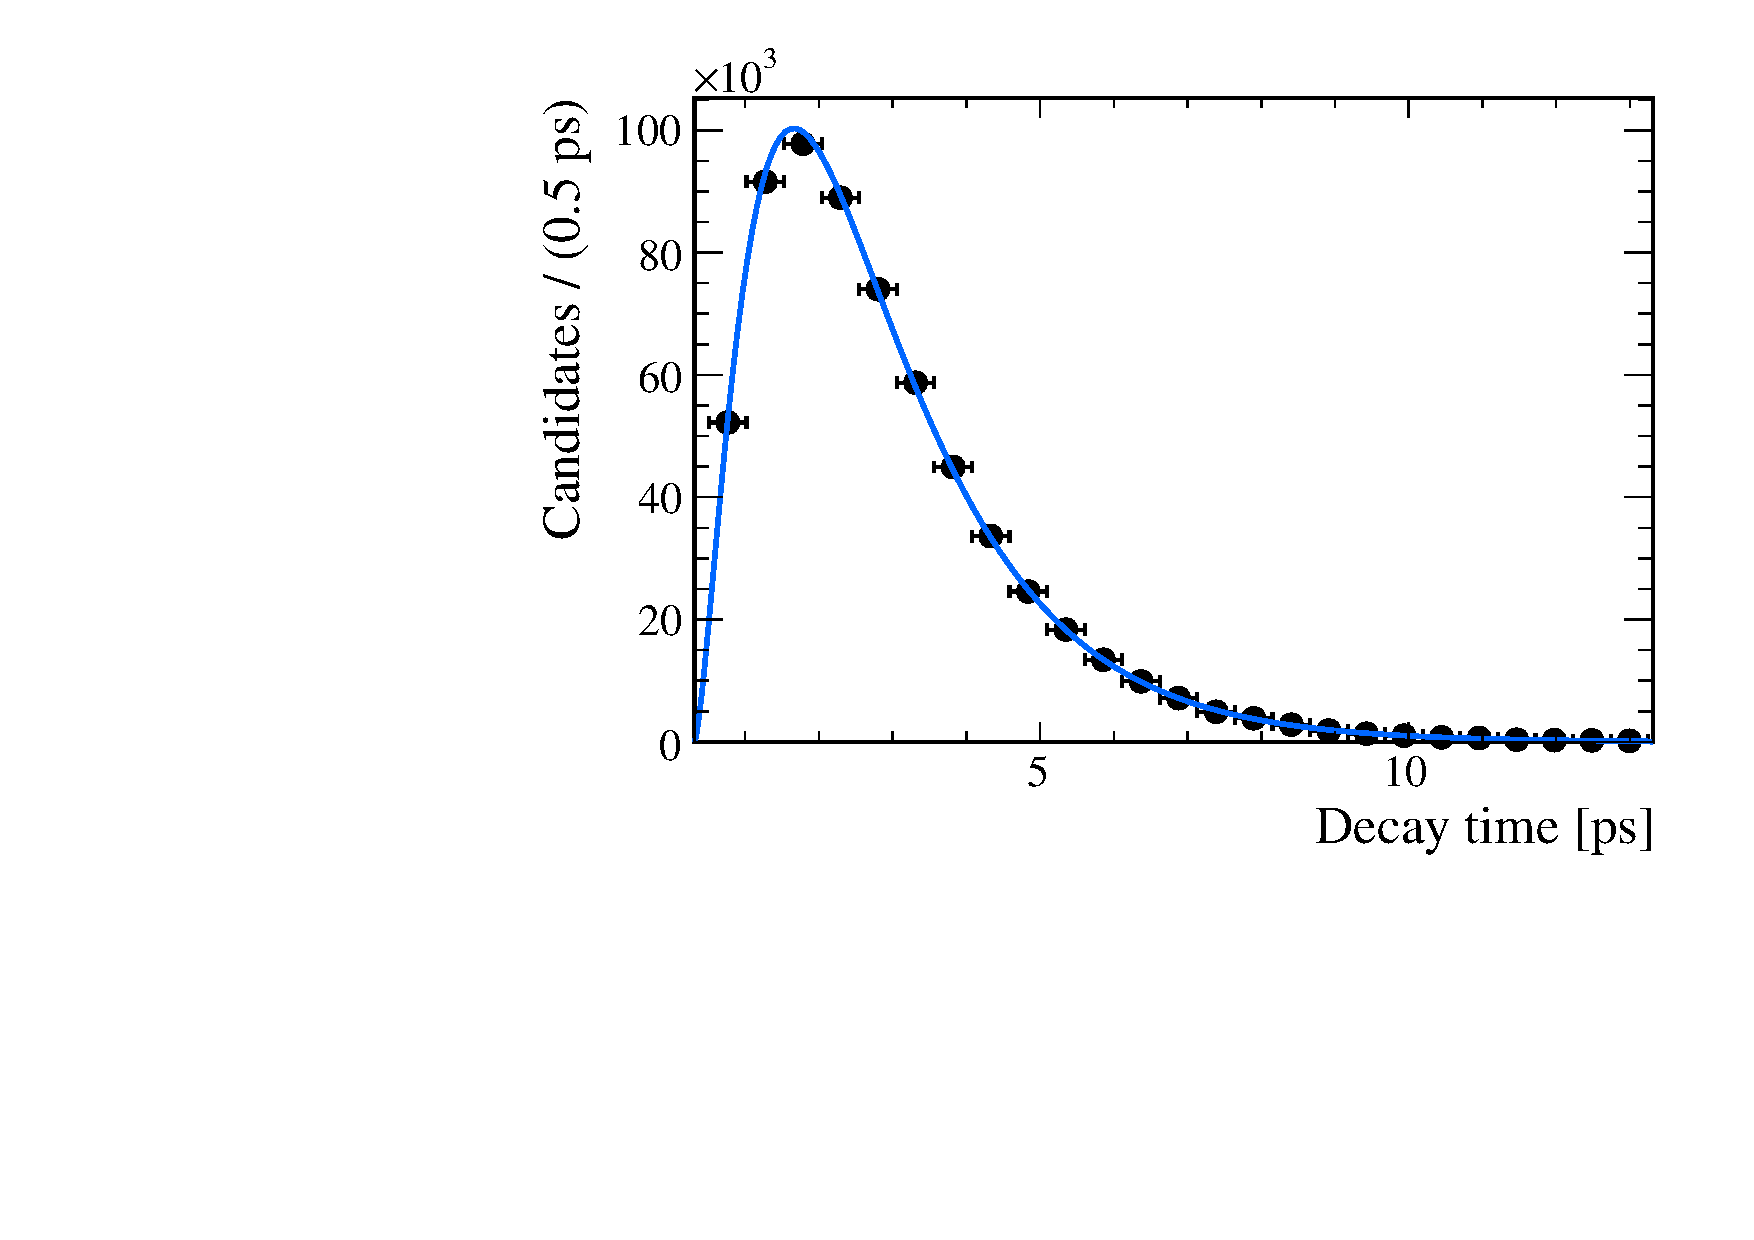
\includegraphics[width= 0.6\textwidth]{./Figs/LifetimeMeasurement/Bs2MuMu_Acceptance_fit.pdf}
       % 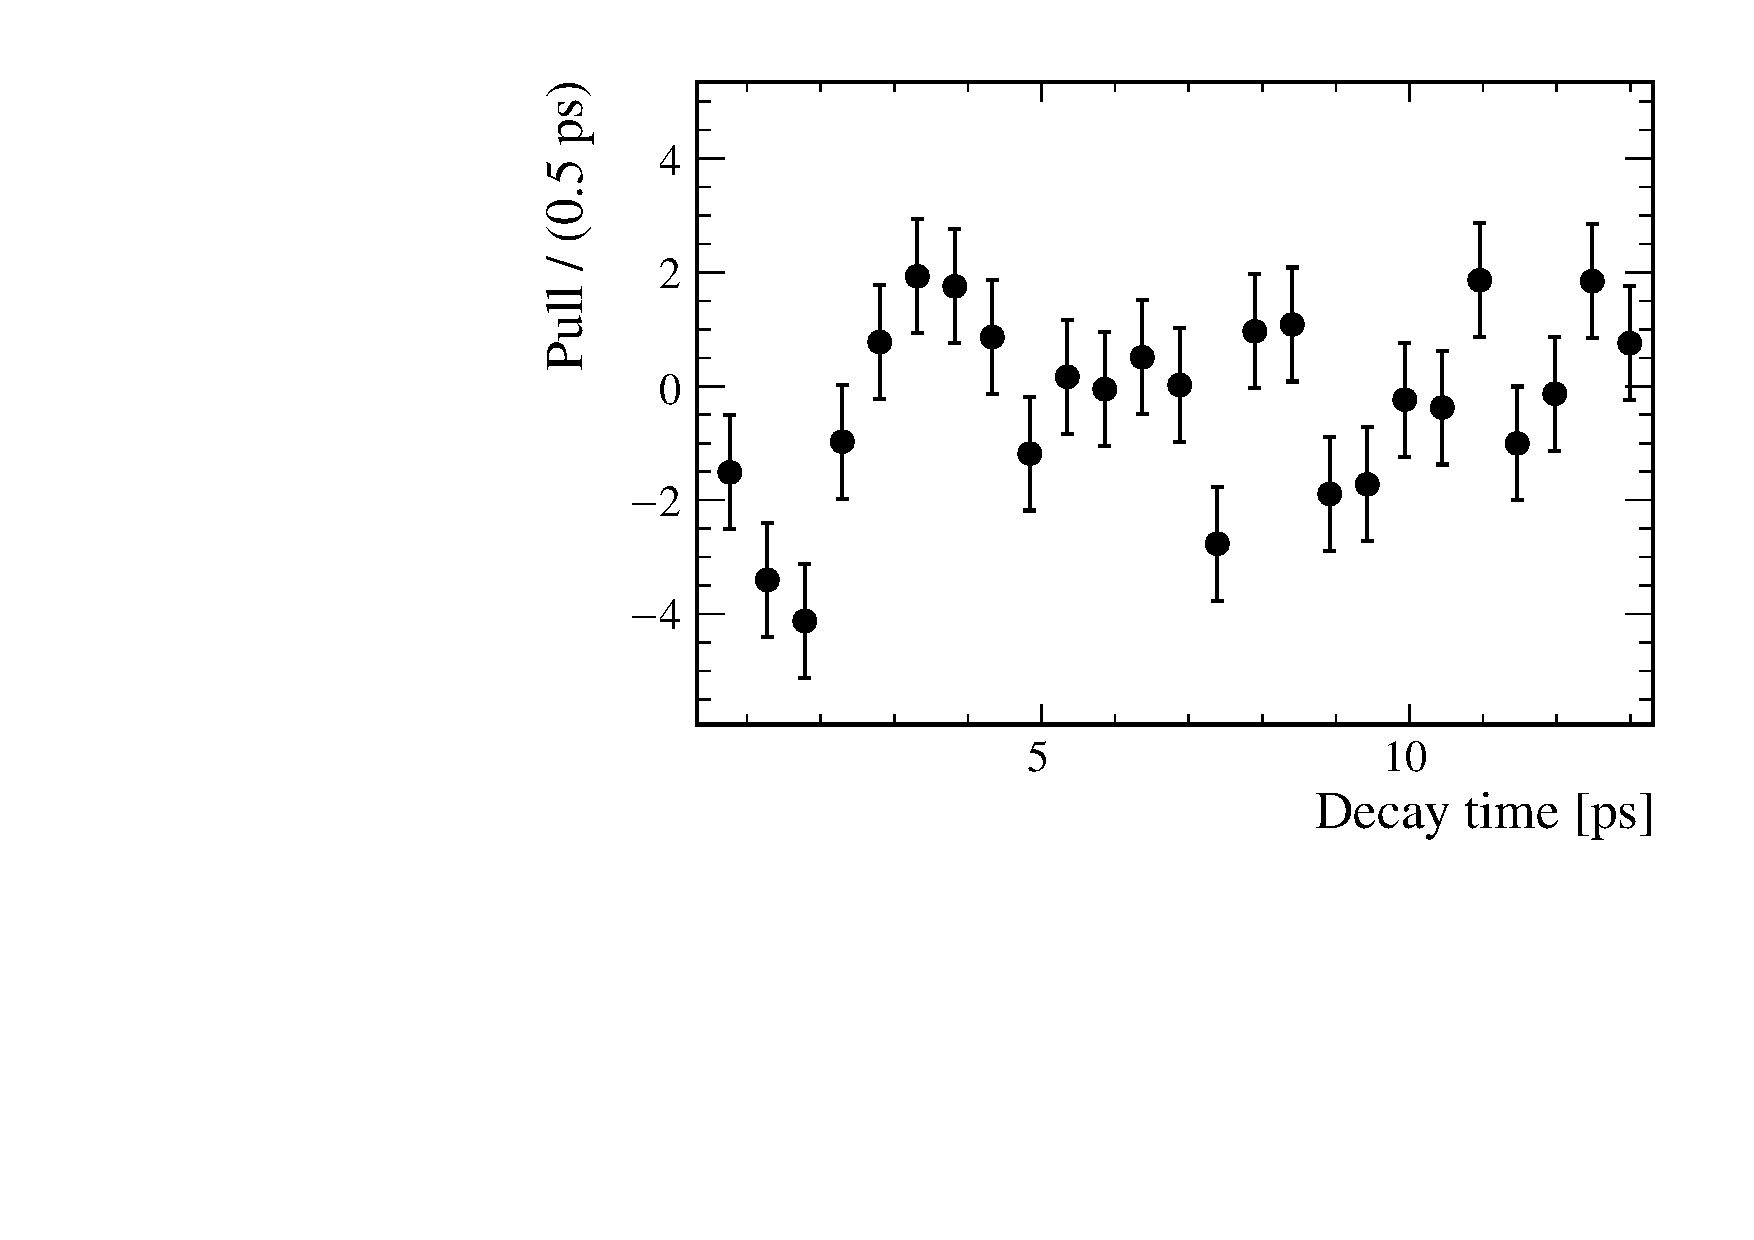
\includegraphics[width= 0.49 \textwidth]{./Figs/LifetimeMeasurement/Bs2MuMu_Accetpance_pull.pdf}
    \caption{Maximum likelihood fit to the combined decay time distribution (left) of 2011, 2012, 2015 and 2016 simulated \bsmumu decays and the pull distribution of the fit. }
    \label{fig:accptfit}
\end{figure}


\begin{figure}[tbp]
    \centering
        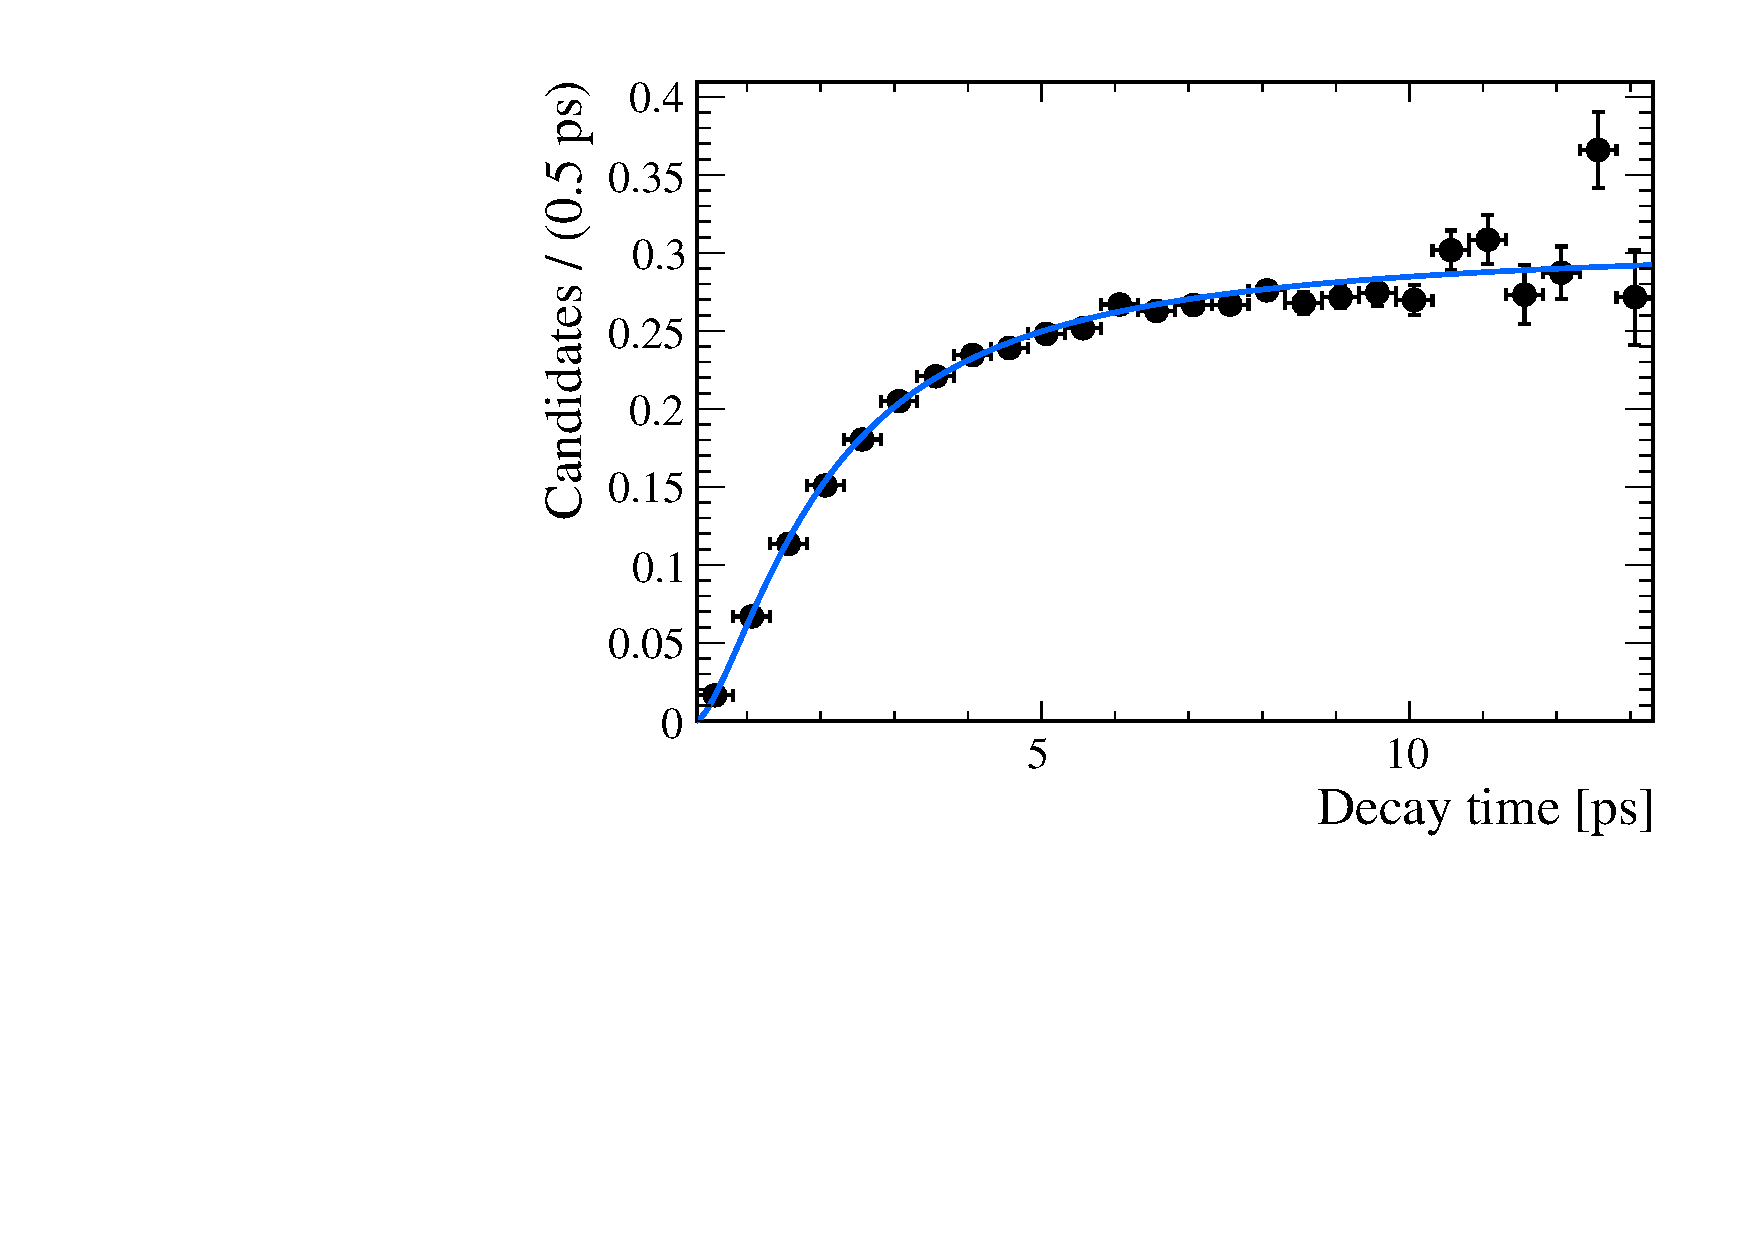
\includegraphics[width= 0.6 \textwidth]{./Figs/LifetimeMeasurement/Bs2MuMu_Acceptance_plot.pdf}
        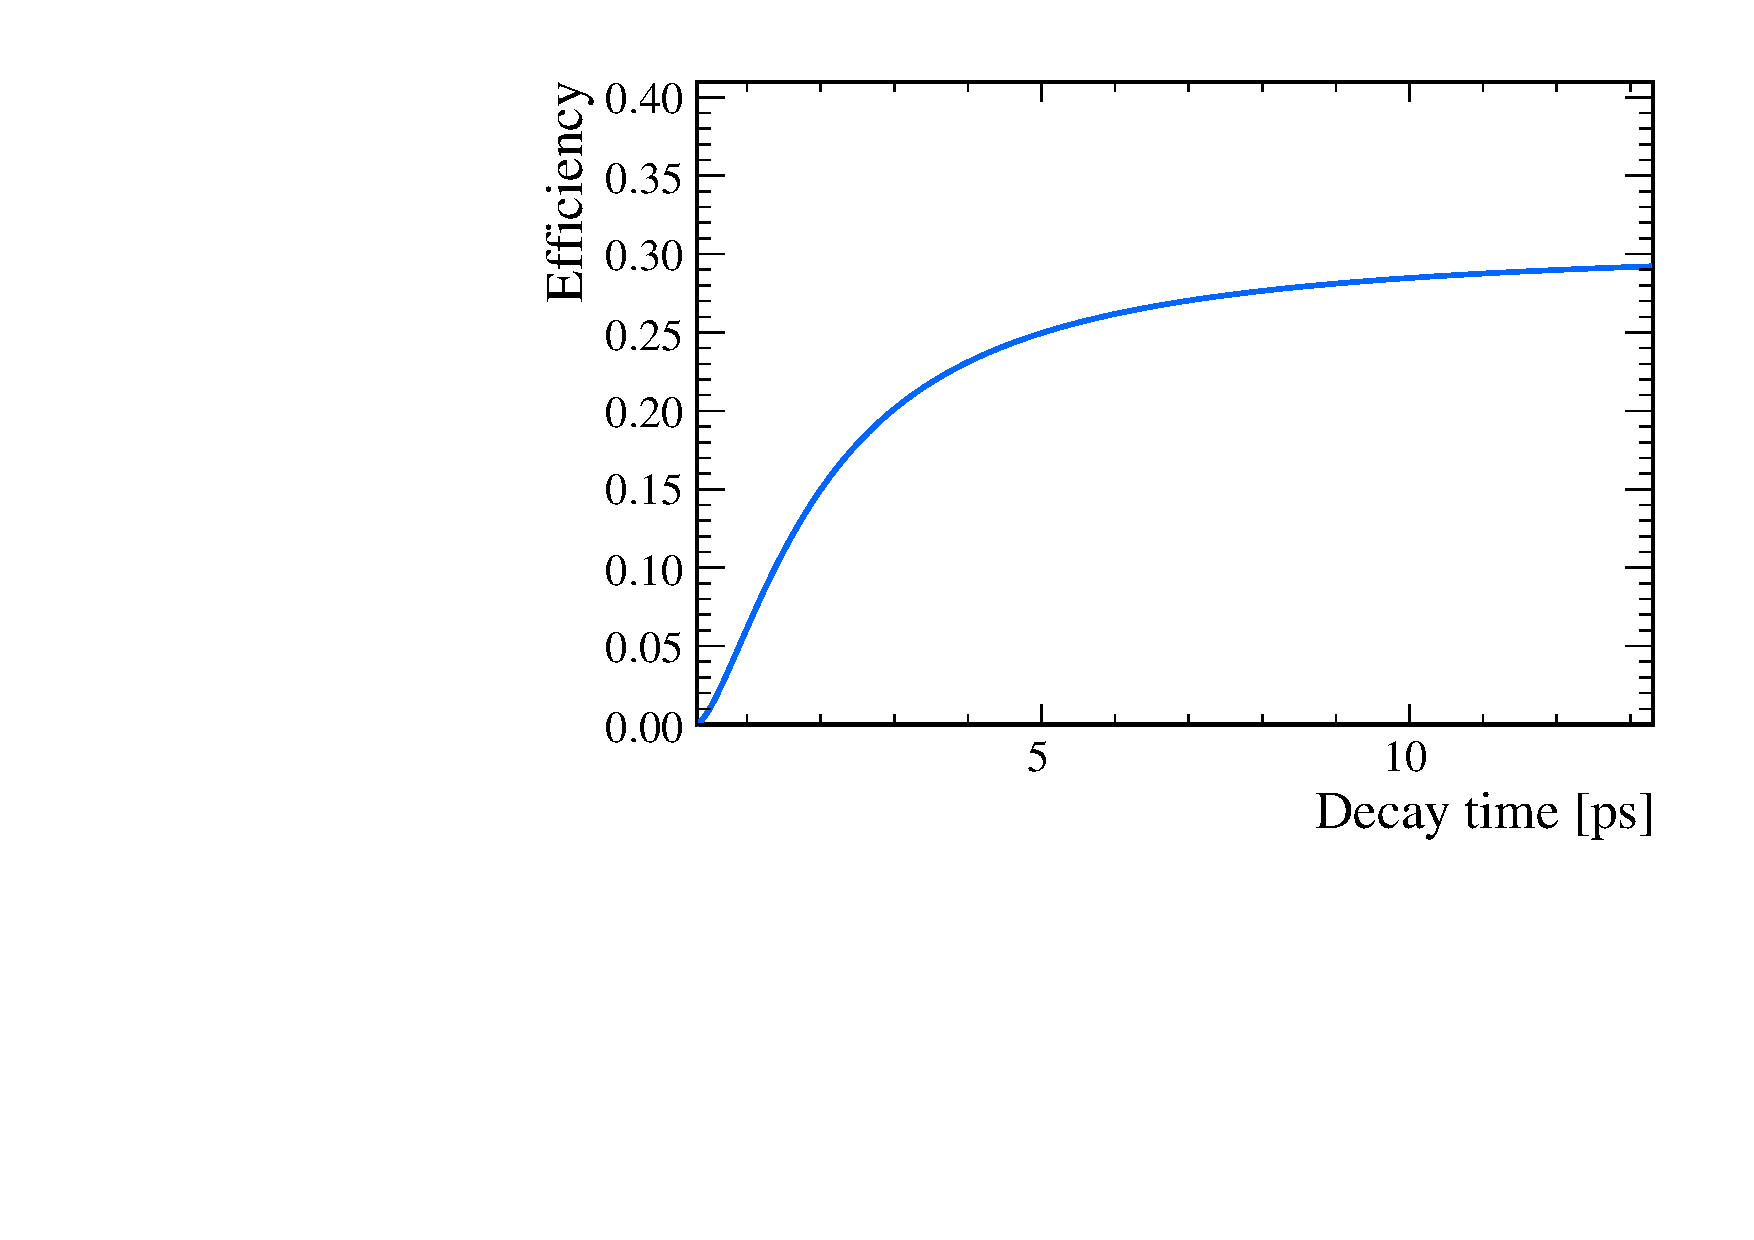
\includegraphics[width= 0.6 \textwidth]{./Figs/LifetimeMeasurement/Bs2MuMu_Acceptance_plot_no_points.pdf}
        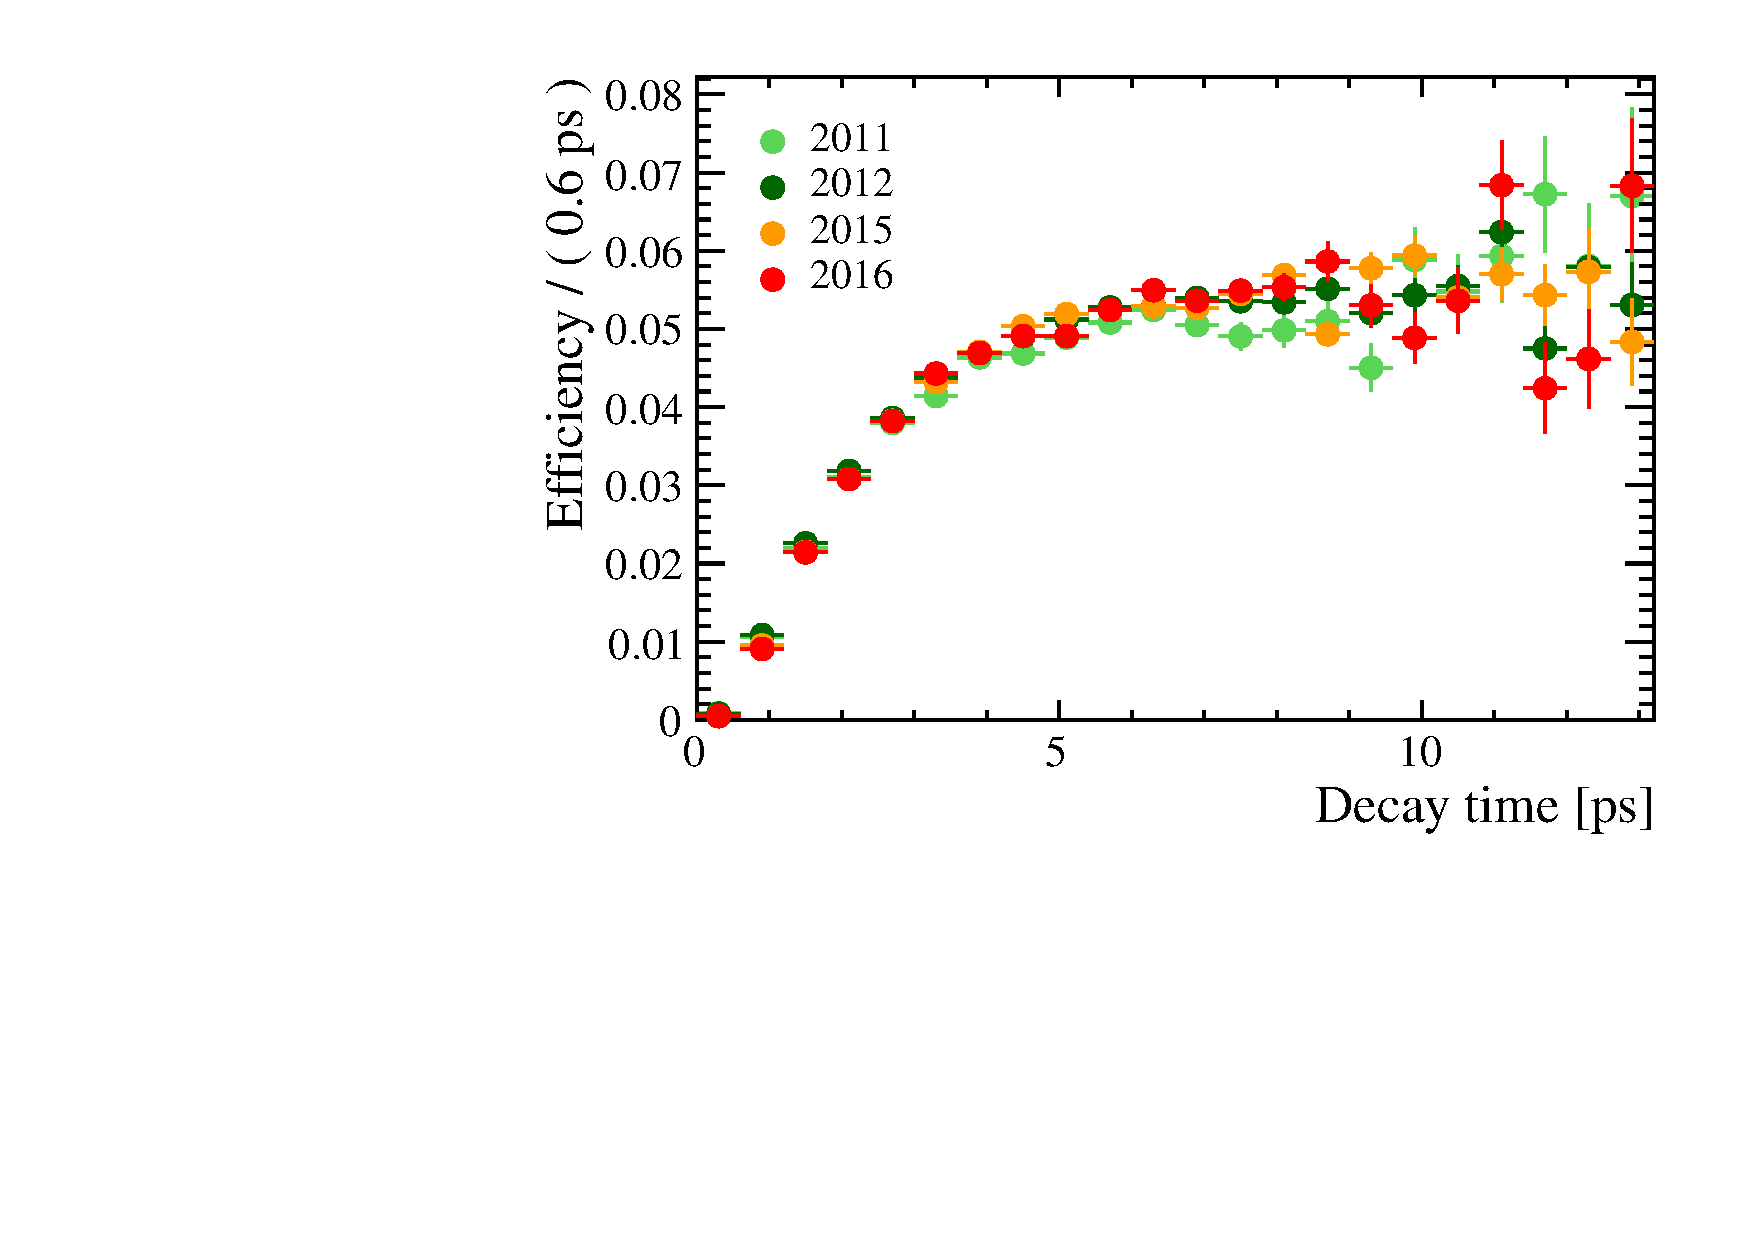
\includegraphics[width= 0.6 \textwidth]{./Figs/LifetimeMeasurement/Acceptance_per_year.pdf}

    \caption{Selection efficiency histogram as a function of decay time with the acceptance \pdf overlaid for weighted 2011, 2012, 2015 and 2016 simulated \bsmumu decays (left) and the efficiency histograms for each year separately for weighted simulated \bsmumu decays. }
    \label{fig:accptplot}
\end{figure}


\begin{table}[tbp]
\begin{center}
\begin{tabular}{lc}
\toprule \toprule
Parameter & Value \\
\midrule
$a$ & 0.574 $\pm$ 0.011 \ps$^{-1}$\\
$n$ & 1.49 $\pm$ 0.03 \\
$t_{0}$ &  0.313 $\pm$ 0.007 \ps \\

\bottomrule \bottomrule
\end{tabular}
\vspace{0.7cm}             
\caption{Parameters for the \bsmumu acceptance function determined from weighted simulated \bsmumu decays.}
\label{tab:accptsig}
\end{center}
\vspace{-1.0cm}                                                                                                                                               
\end{table}

\subsection{Background decay time \pdfs}
\label{sec:bkgDTpdf}

The final fit to measure the \bsmumu effective lifetime does not require knowledge of the decay time \pdfs of the backgrounds. However, the fit configuration is developed using toy studies that use the mass and decay time distributions of both signal and background decays. Therefore realistic models of the decay time \pdfs are needed to determine the optimal fit configuration. 


The selection biases the decay time distributions of the backgrounds in the same way as the \bsmumu decay time. Therefore, they are described by the same \pdfs as in Equation~\ref{eq:DTpdf}. 

The backgrounds from mis-identified and \bdmumu decays are assigned the same acceptance function as \bsmumu decays, Equation~\ref{eq:accpt}, because the decay time efficiency of these backgrounds is approximately the same as the signal. The acceptances of these backgrounds does not need to be as accurately known as the acceptance function of the signal because very few background decays from these sources will be present in the dataset after the selection and the final result does not depend on the acceptance function of the backgrounds. The lifetimes of these background decays are taken from a fit to simulated decays. For \bhh the fit is performed to a combined set of \bhh decays representing what is expected in data. %the values used in the toy studies for the decay times \pdfs are given in Table~\ref{}. 

The decay time \pdf of the combinatorial background is more challenging to determine. This background arises from random combinations of muons in the event and not from one source, therefore there is no single lifetime that describes the background. Furthermore, the global BDT which is designed to separate \bsmumu decays from combinatorial background decays will have a different efficiency as a function of decay time for the combinatorial background compared to the \bsmum signal. The decay time \pdf of the combinatorial background cannot be evaluated from simulated decays or decays in data that pass the \bsmumu selection because there are too few candidates left. %The decay time \pdf must be evaluated after the global BDT cut because it has the greatest impact on the shape of the acceptance function. 
Therefore, the decay time \pdf of the combinatorial background for \bsmumu decays is evaluated from the combinatorial background of \bhh decays using candidates in data that pass the \bhh selection and have a reconstructed mass greater than 5447 \mevcc, above the \bs signal region. The decay time \pdf for combinatorial background decays is modelled by
\begin{equation}
P_{cbg}(t) = \epsilon(t)\times \left( f \cdot e^{-t/\tau_{1}} + (1-f)\cdot e^{-t/\tau_{2}} \right)
\label{eq:cbgDTpdf}
\end{equation}
where $\tau_{1}$ and $\tau_{2}$ are two independent lifetimes used to describe the background, $f$~describes the fraction of candidates with lifetime $\tau_{1}$ and the same acceptance shape as in Equation~\ref{eq:accpt} is used for describe the decay time efficiency $\epsilon(t)$. The lifetimes are different, one describes a long-lived component and the other a short-lived component that are evident in the data. The decay time acceptance is flat at large decay times, therefore the lifetimes of the combinatorial background decays are determined from a \ml fit using Equation~\ref{eq:cbgDTpdf}, setting $\epsilon(t)=1$, to candidates with a decay time above 2.5~\ps. The acceptance function parameters are then determined from a \ml fit to the full decay time range using Equation~\ref{eq:cbgDTpdf}, where the lifetimes and the fraction of candidates with each lifetime are fixed. The results are shown in Figure~\ref{fig:CBGaccpt} and the \pdf parameters in Table~\ref{tab:bkgparams}, the $t_{0}$ parameter is fixed in the fit to improve fit stability. 
\begin{table}[tbp]
\begin{center}
\begin{tabular}{lc}
\toprule \toprule
Parameter & Value \\
\midrule
$a$ & 1.45 $\pm$ 0.12 \ps$^{-1}$\\
$n$ & 1.92 $\pm$ 0.17 \\
$t_{0}$ & 0.290 \ps \\
$\tau_{1}$ & $17 \pm 16$ \ps \\ 
$\tau_{2}$ & $1.3 \pm 0.3$ \ps \\
$f$ & 0.032 $\pm$ 0.027 \\
\bottomrule \bottomrule
\end{tabular}
\vspace{0.7cm}             
\caption{Parameters used to described the background decay time distribution from combinatorial background decays in data passing the \bhh selection.}
\label{tab:bkgparams}
\end{center}
\vspace{-1.0cm}                                                                                                                                               
\end{table}

\begin{figure}[tbp]
    \centering
   \begin{subfigure}[b]{0.48\textwidth}
        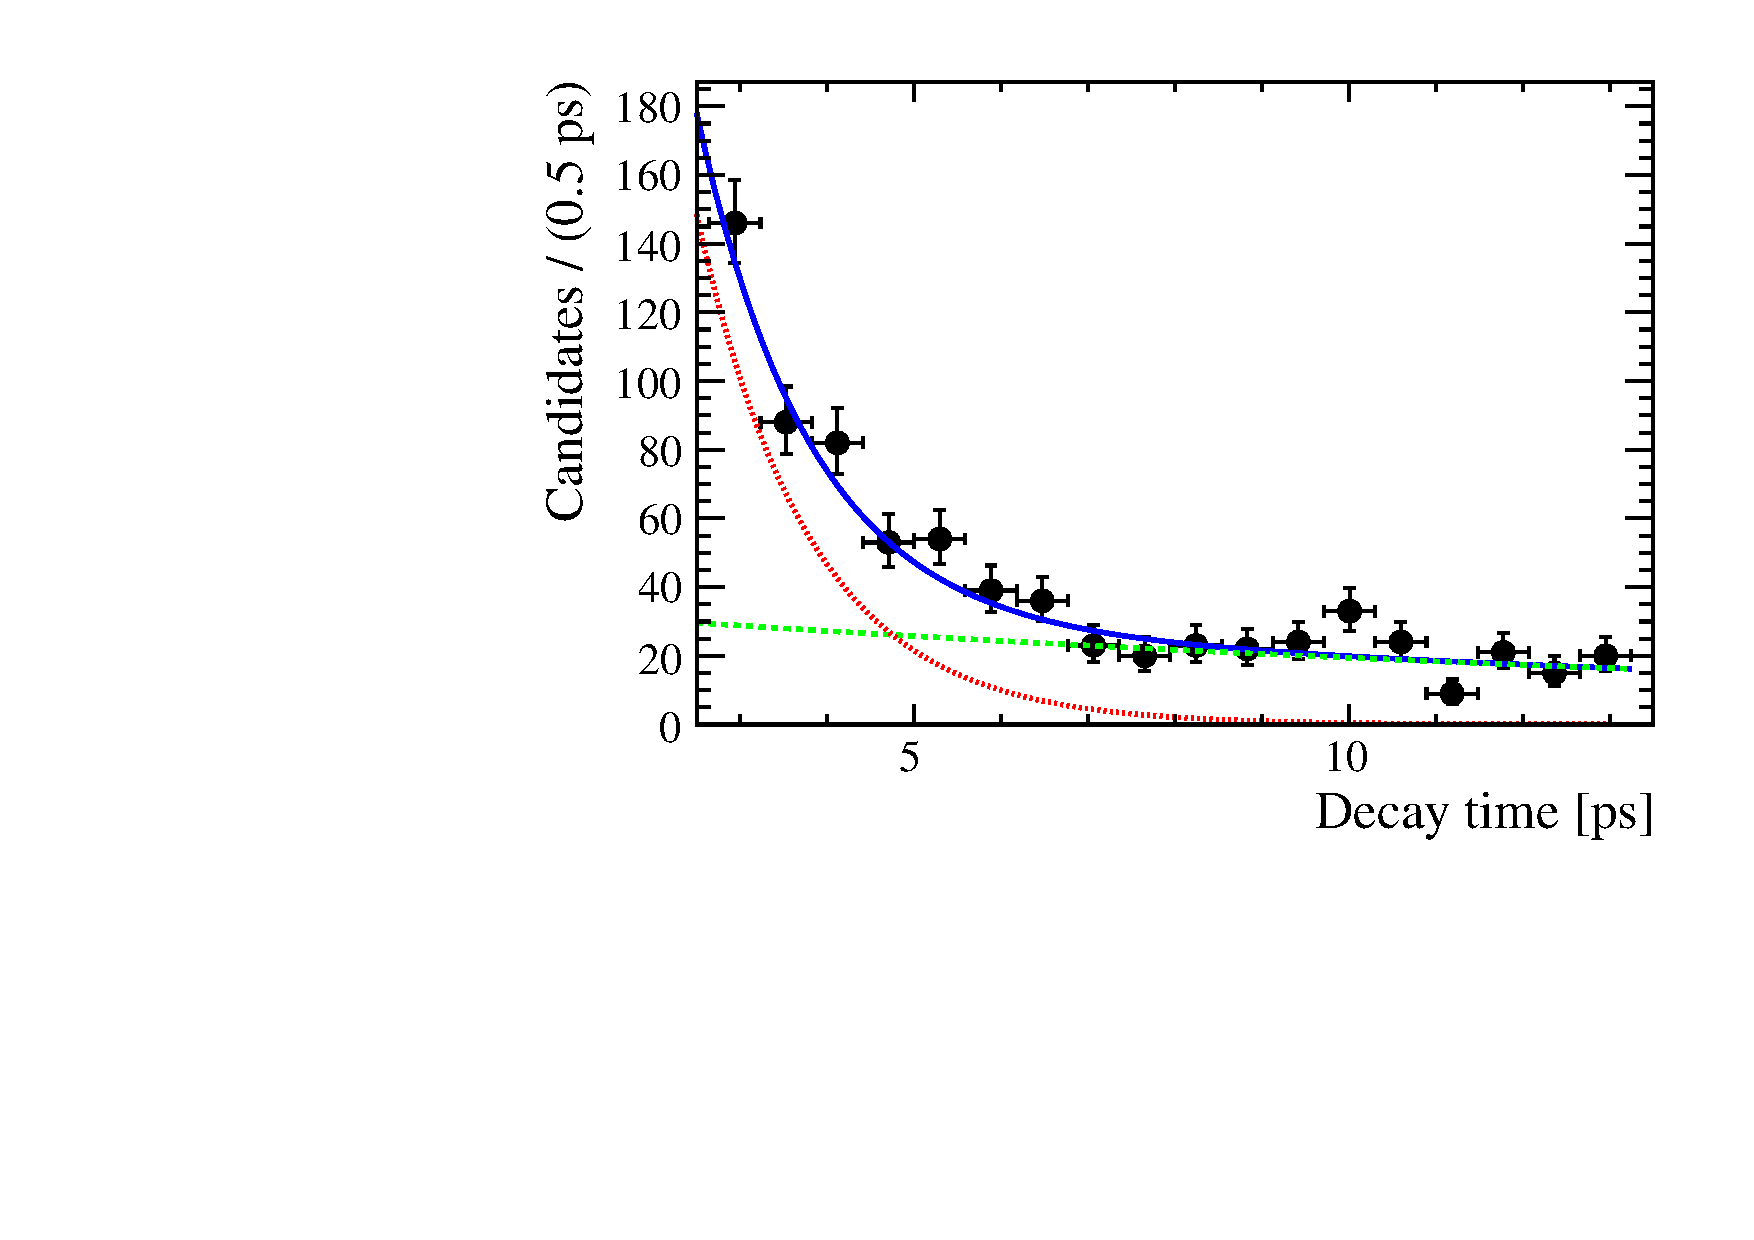
\includegraphics[width= \textwidth]{./Figs/LifetimeMeasurement/CBG_slope_fit.pdf}
        %\caption{ }                                                                                                                    
        %\label{fig:BDTSsig}                                                                                                            
    \end{subfigure}
   ~ %add desired spacing between images, e. g. ~, \quad, \qquad, \hfill etc.                                                         
      %(or a blank line to force the subfigure onto a new line)                                                                         
    \begin{subfigure}[b]{0.48\textwidth}
       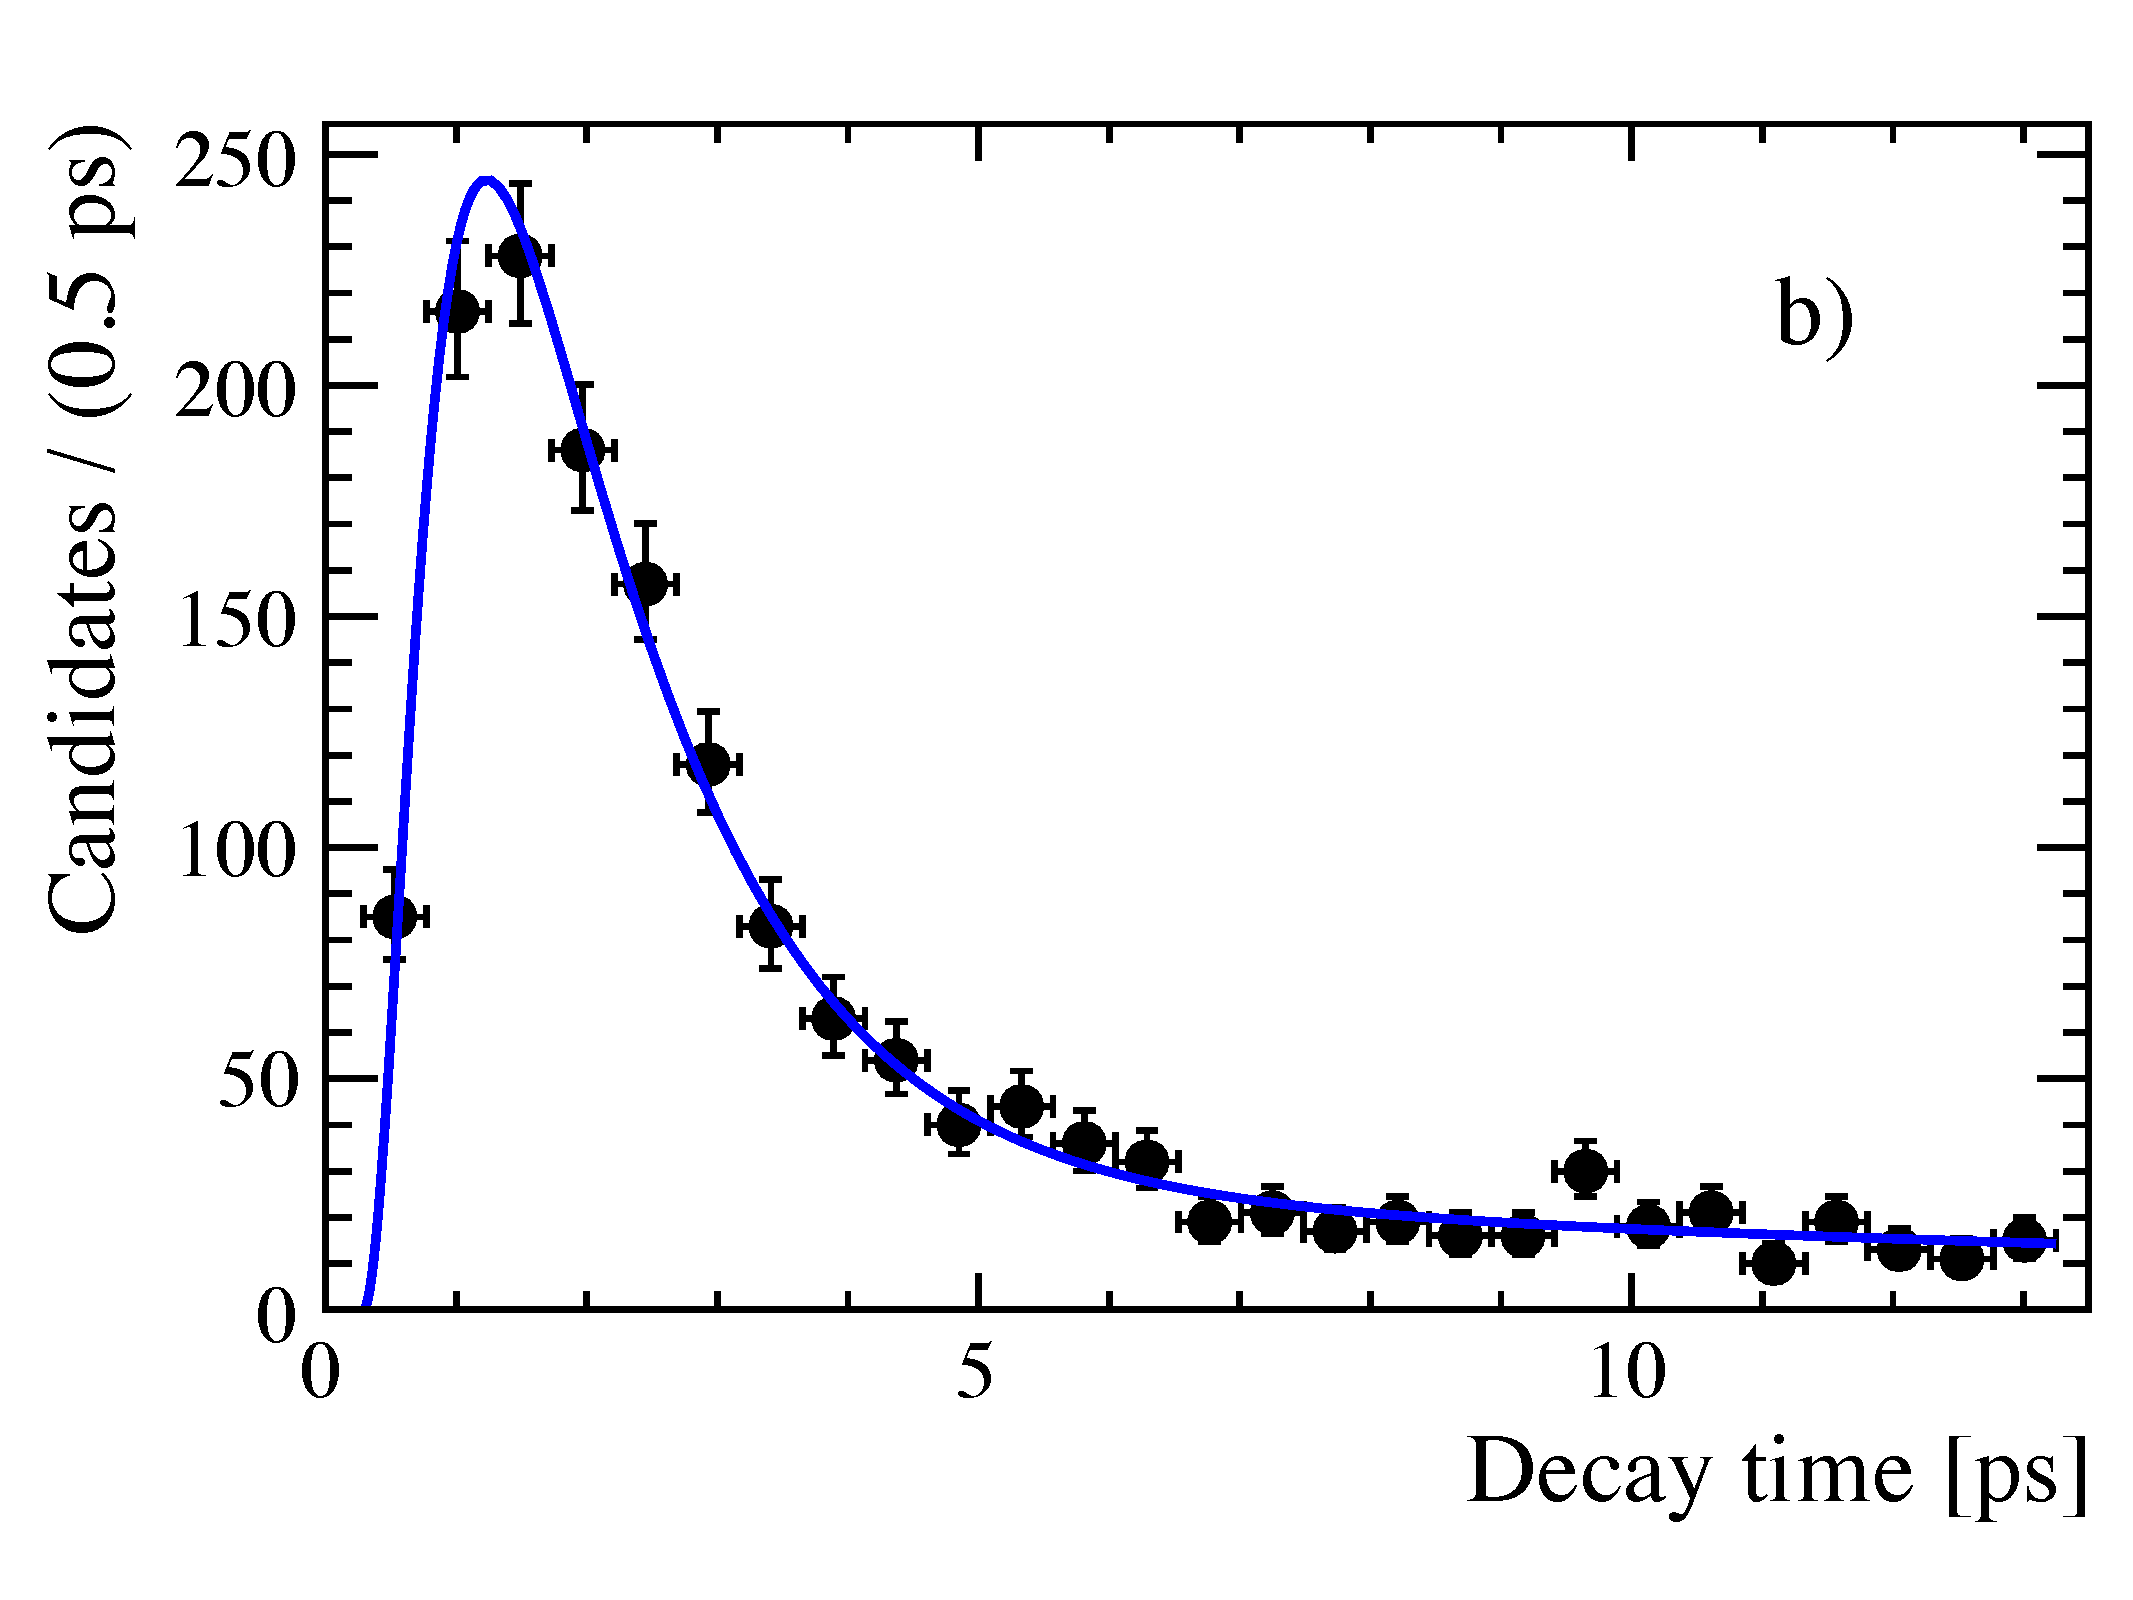
\includegraphics[width=\textwidth]{./Figs/LifetimeMeasurement/CBG_accpt_fit.pdf}
      %  \caption{ }                                                                                                                    
     %   \label{fig:BDTSbkg}                                                                                                            
   \end{subfigure}
    \caption{Maximum likelihood fit to determine the lifetimes of the background (top), with the long live component (bottom) and the short-lived component (red). The decay time distribution acceptance (right) of the combinatorial background decays in data passing the \bhh selection requirements.}
    \label{fig:CBGaccpt}
\end{figure}

This model for the background assumes that the decay time distribution of \bhh candidates formed by random combinations of kaons and pions is the same as that of \bsmumu candidates formed by randomly combining muons in the event. There are too few candidates passing the \bsmumu selection to verify this assumption, although the validity of this model and the impact of the toy studies is investigated in Section~\ref{sec:CBGdecytimemodel}.%however the average decay time of \bhh and \bsmumu candidates with a mass above 5600 \mevcc is evaluated in bins of BDT. The results are shown in Table~\ref{}, the average decay times are not significantly different for \bhh and \bsmumu candidates therefore the decay time \pdf described here is a good model for the combinatorial background in the toy studies.


\section{Fit optimisation}
\label{sec:toys}
The strategy to measure the \bsmumu effective lifetime was described in Section~\ref{sec:fitstrategy}. However, given the extremely rare nature of \bsmumu decays, the stability and performance of the final fit will be highly dependant on the fit to the invariant mass distribution. Pseudoexperiments were performed to determine which mass range would produce an accurate fit with the smallest expected uncertainty on the measured effective lifetime for the dataset. The choice of the mass range determines which background sources need to be included into the fit.


The expected number of signal and background decays in the data set passing the \bsmumu selection in the mass range 4600 - 6000 \mevcc were used as the basis for the toy studies. The expected background yields were calculated using the same methods described in Section~\ref{sec:backgrounds} but taking into account the looser particle identification requirement and the cut placed on the global BDT. The number of \bsmumu and \bdmumu decays are calculated using the normalisation factors in Section~\ref{sec:Normalisation} and assuming the branching fraction values predicted by the SM. The expected yields are shown in Table~\ref{tab:expectedevents}. 


\begin{table}[ht]
\begin{center}
\begin{tabular}{lc}
\toprule \toprule
Decay & Expected yield \\ \midrule
\bsmumu & 30.94\\ 
\bdmumu & 3.27\\ 
\bhh & 9.68\\ 
\lambdab &  13.34\\ 
\bdpimunu & 40.50 \\ 
\bsKmunu &  9.13\\ 
\bupimumu &  6.01\\ 
\bdpimumu  &  4.86\\ 
\bcjpsimunu  &  9.79\\ 
Combinatorial background & 66.23\\ 
\bottomrule \bottomrule
\end{tabular}
\vspace{0.7cm}                                                                                                                                               
\caption{Number of expected decays in data passing the \bsmumu effective lifetime selection.}
\label{tab:expectedevents}
\end{center}
\vspace{-1.0cm}                                                                                                                                               
\end{table}


The toy studies are performed by generating the mass and decay time distributions for the expected number of signal and background decays using the \pdfs described in Section~\ref{sec:ELmasspdfs} and~\ref{sec:DTpdfs}, assuming the Standard Model prediction for \tmumu, and taking the slope of the combinatorial background mass \pdf from simulated decays. sWeights are computed from an unbinned \ml fit to the invariant mass distribution. The lifetime and its inverse are measured by a unbinned \ml fit to the sWeighted decay time distribution. A series of different mass ranges and background components were tested. For each possible configuration a study containing 10,000 pseudoexperiments were performed and the performance of each configuration was evaluated using a couple of different metrics. The first, is the median expected uncertainty of the \bsmumu lifetime and inverse lifetime, the median rather than the mean uncertainty is used due to the asymmetric spread of uncertainties observed for the expected statistics. The second measure, is the pull distributions of any free parameters in the fit, where the pull is defined as $(x - \mu)/\sigma$ with $x$ the measured parameter value, $\mu$ the value used in the generation and $\sigma$ the uncertainty on the measured parameter value. Ideally the pull distributions will be Gaussian in shape with a mean at 0 and a width of 1.

 The details of the toy studies performed are given in Section~\ref{sec:toyresults}. However first is a discussion of whether the lifetime or inverse lifetime should be measured given the expected number of decays present in the data set.  

\subsection{To fit for $\tau$ or $\tau^{-1}$?}
\label{sec:tauORinvtau}
During the development of the fit strategy, the toy studies produced biased pull distributions for the measured \bsmumu effective lifetime no matter what mass fit configuration or acceptance function was used. The pull distribution for the effective lifetime, \tmumu, is shown in Figure~\ref{fig:taupulls} for a simplified configuration where no acceptance function is used and only signal and combinatorial background decays are generated in the mass range 4900 - 6000 \mevcc. The distribution is clearly not Gaussian in shape. The bias was more pronounced in early stages of the analysis development which was performed assuming the expected signal and background yields of only the Run 1 data set.%, also shown in Figure~\ref{fig:taupulls}. 

\begin{figure}[tbp]
    \centering
    \begin{subfigure}[b]{0.49\textwidth}
        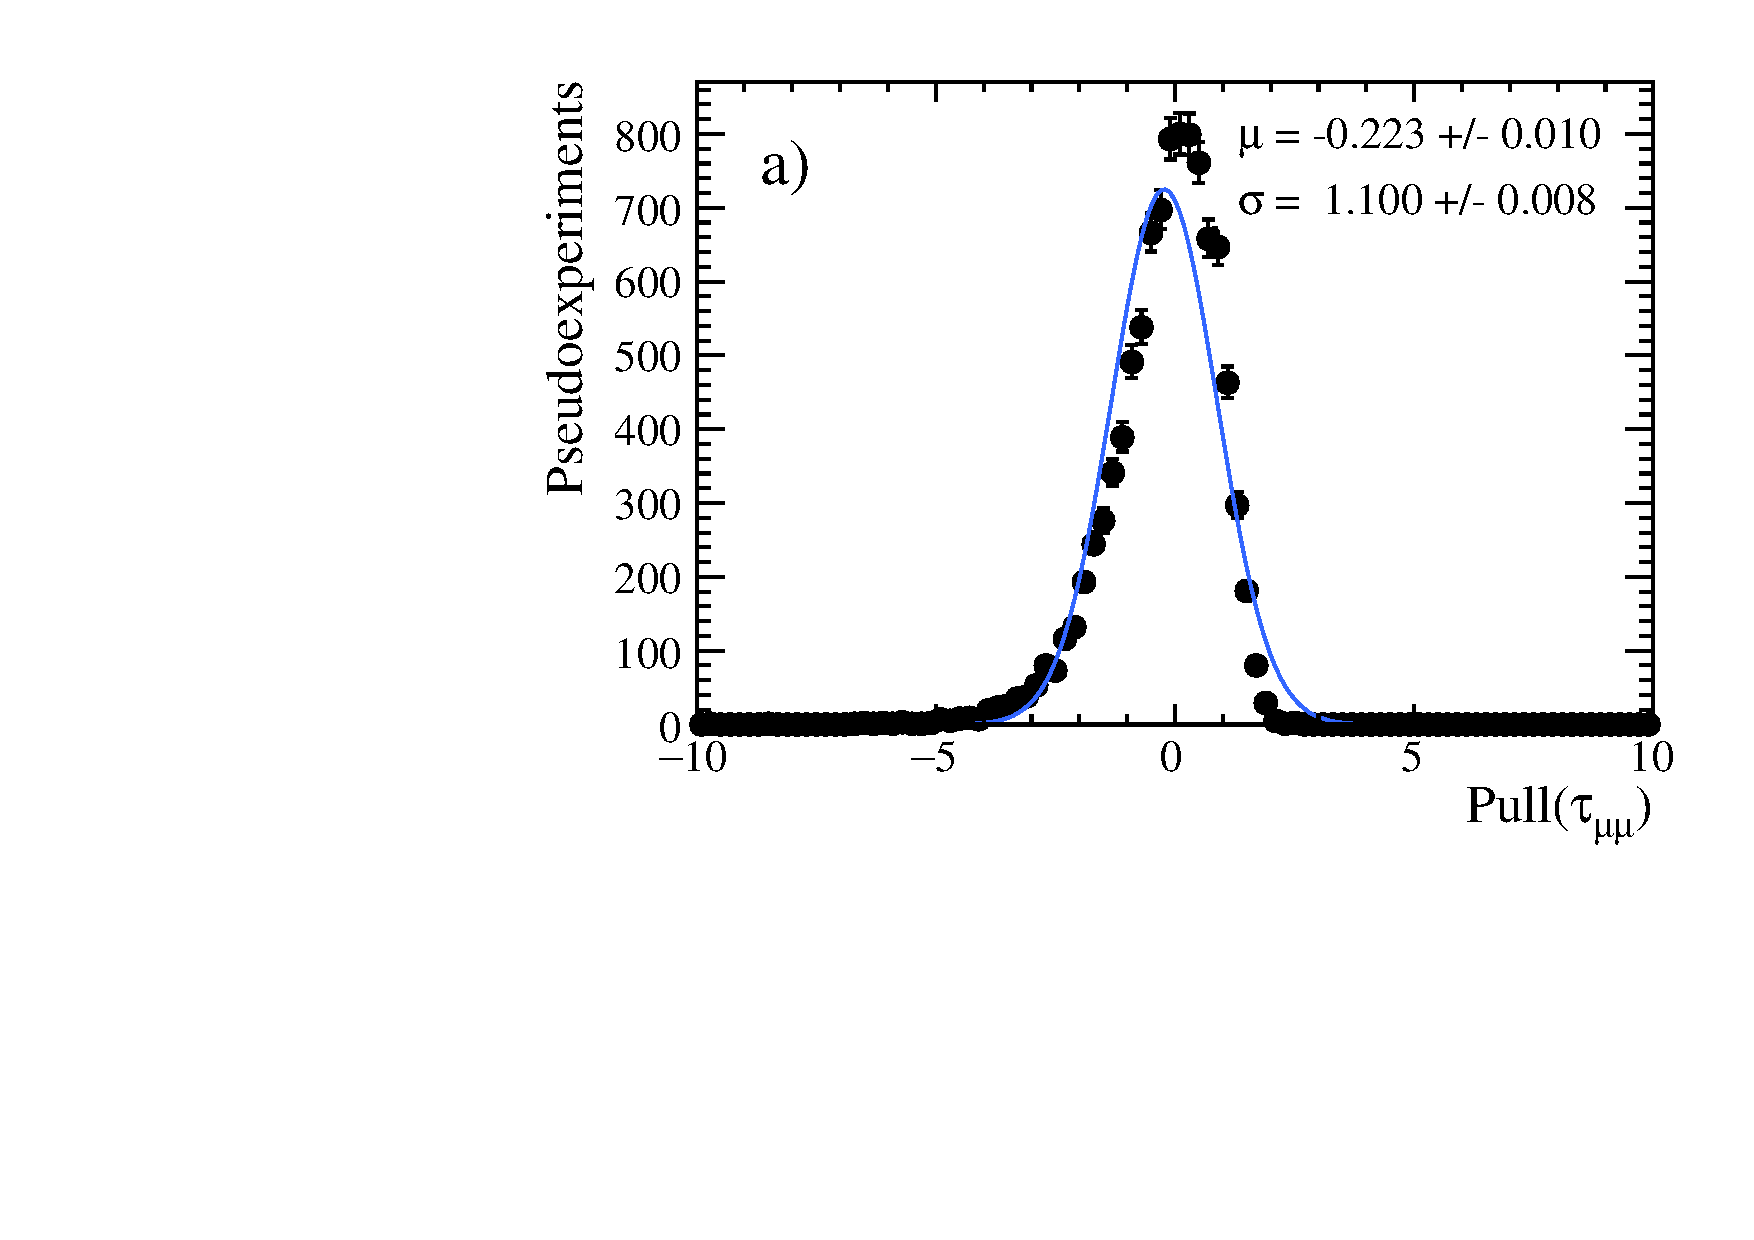
\includegraphics[width=  \textwidth]{./Figs/LifetimeMeasurement/CKM_simple_tau_pull.pdf} 
         \label{fig:tau_pull}
    \end{subfigure}
    \begin{subfigure}[b]{0.49\textwidth}
      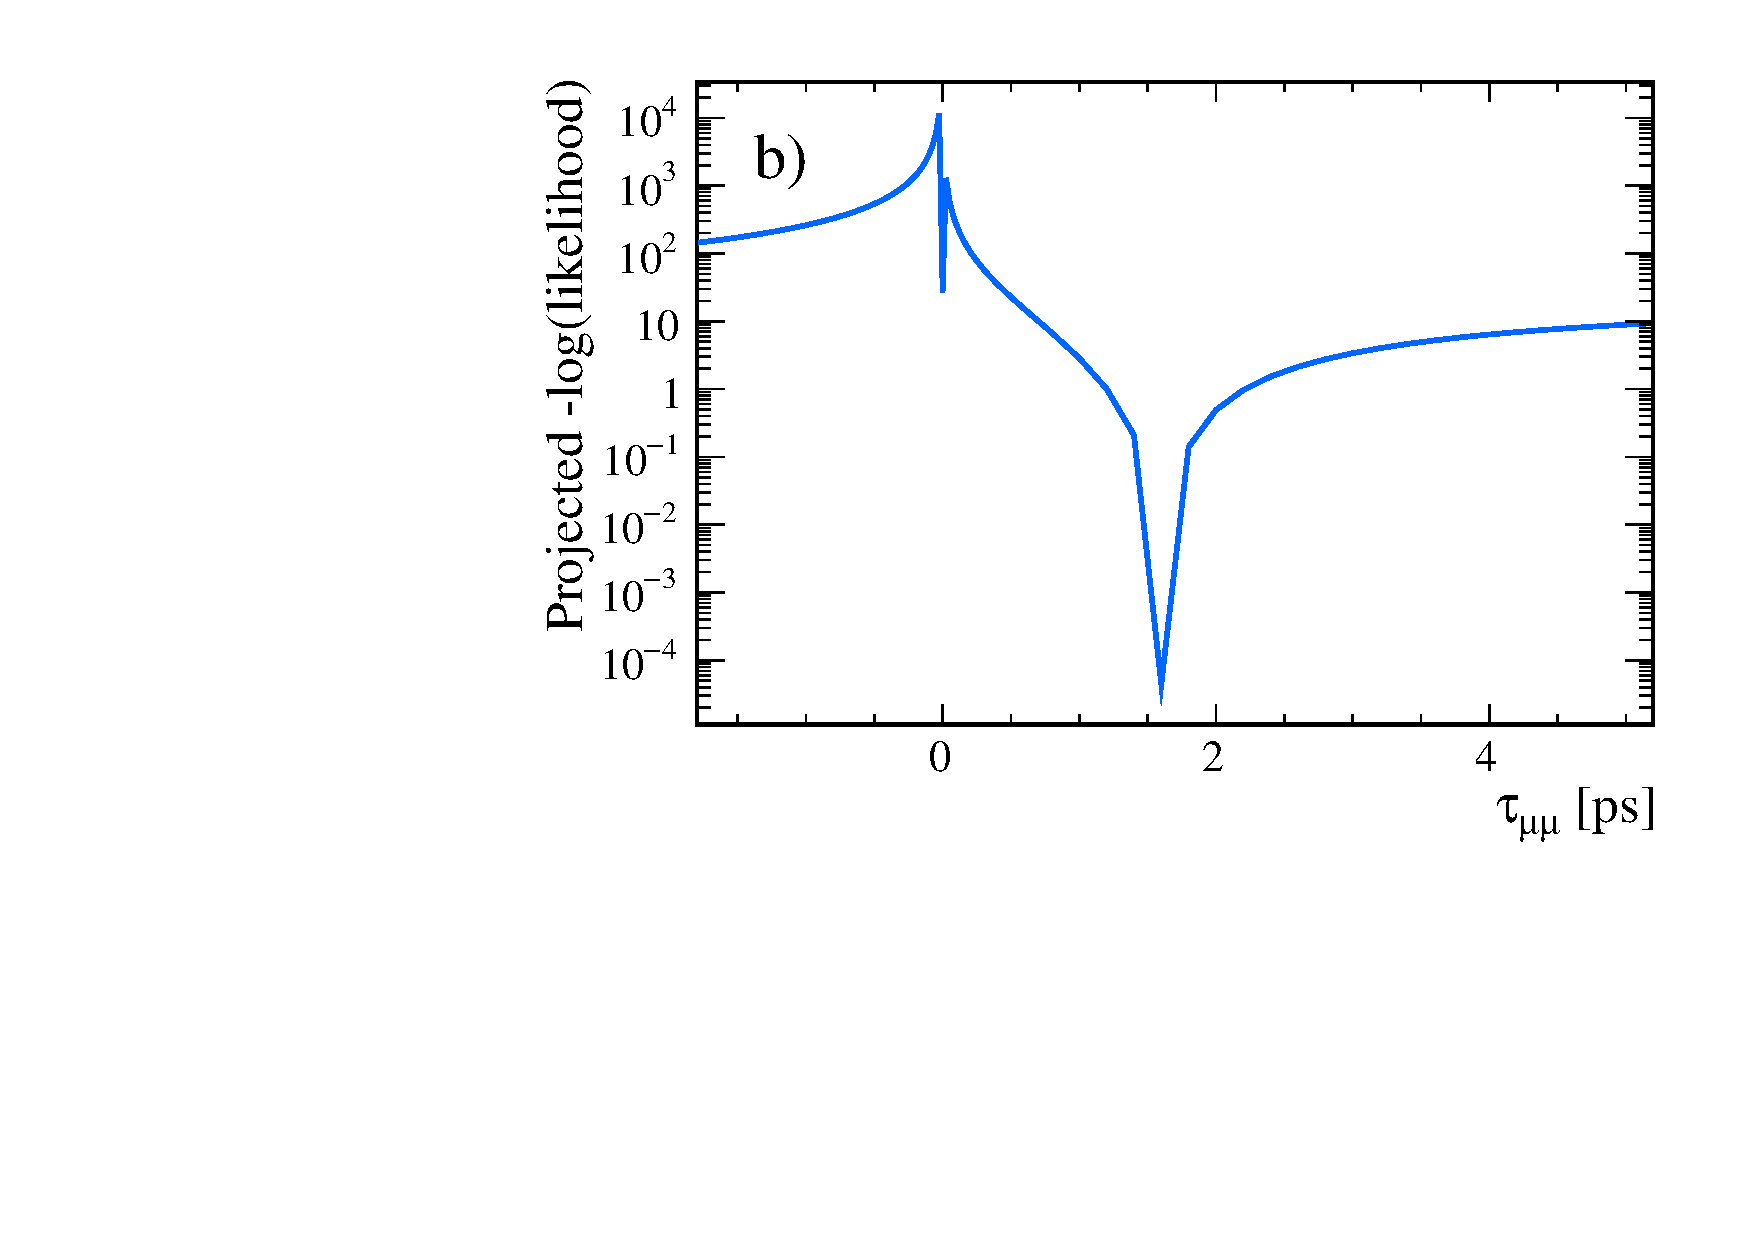
\includegraphics[width=  \textwidth]{./Figs/LifetimeMeasurement/tau_LL.pdf}  
         \label{fig:tau_ll}
    \end{subfigure}
        %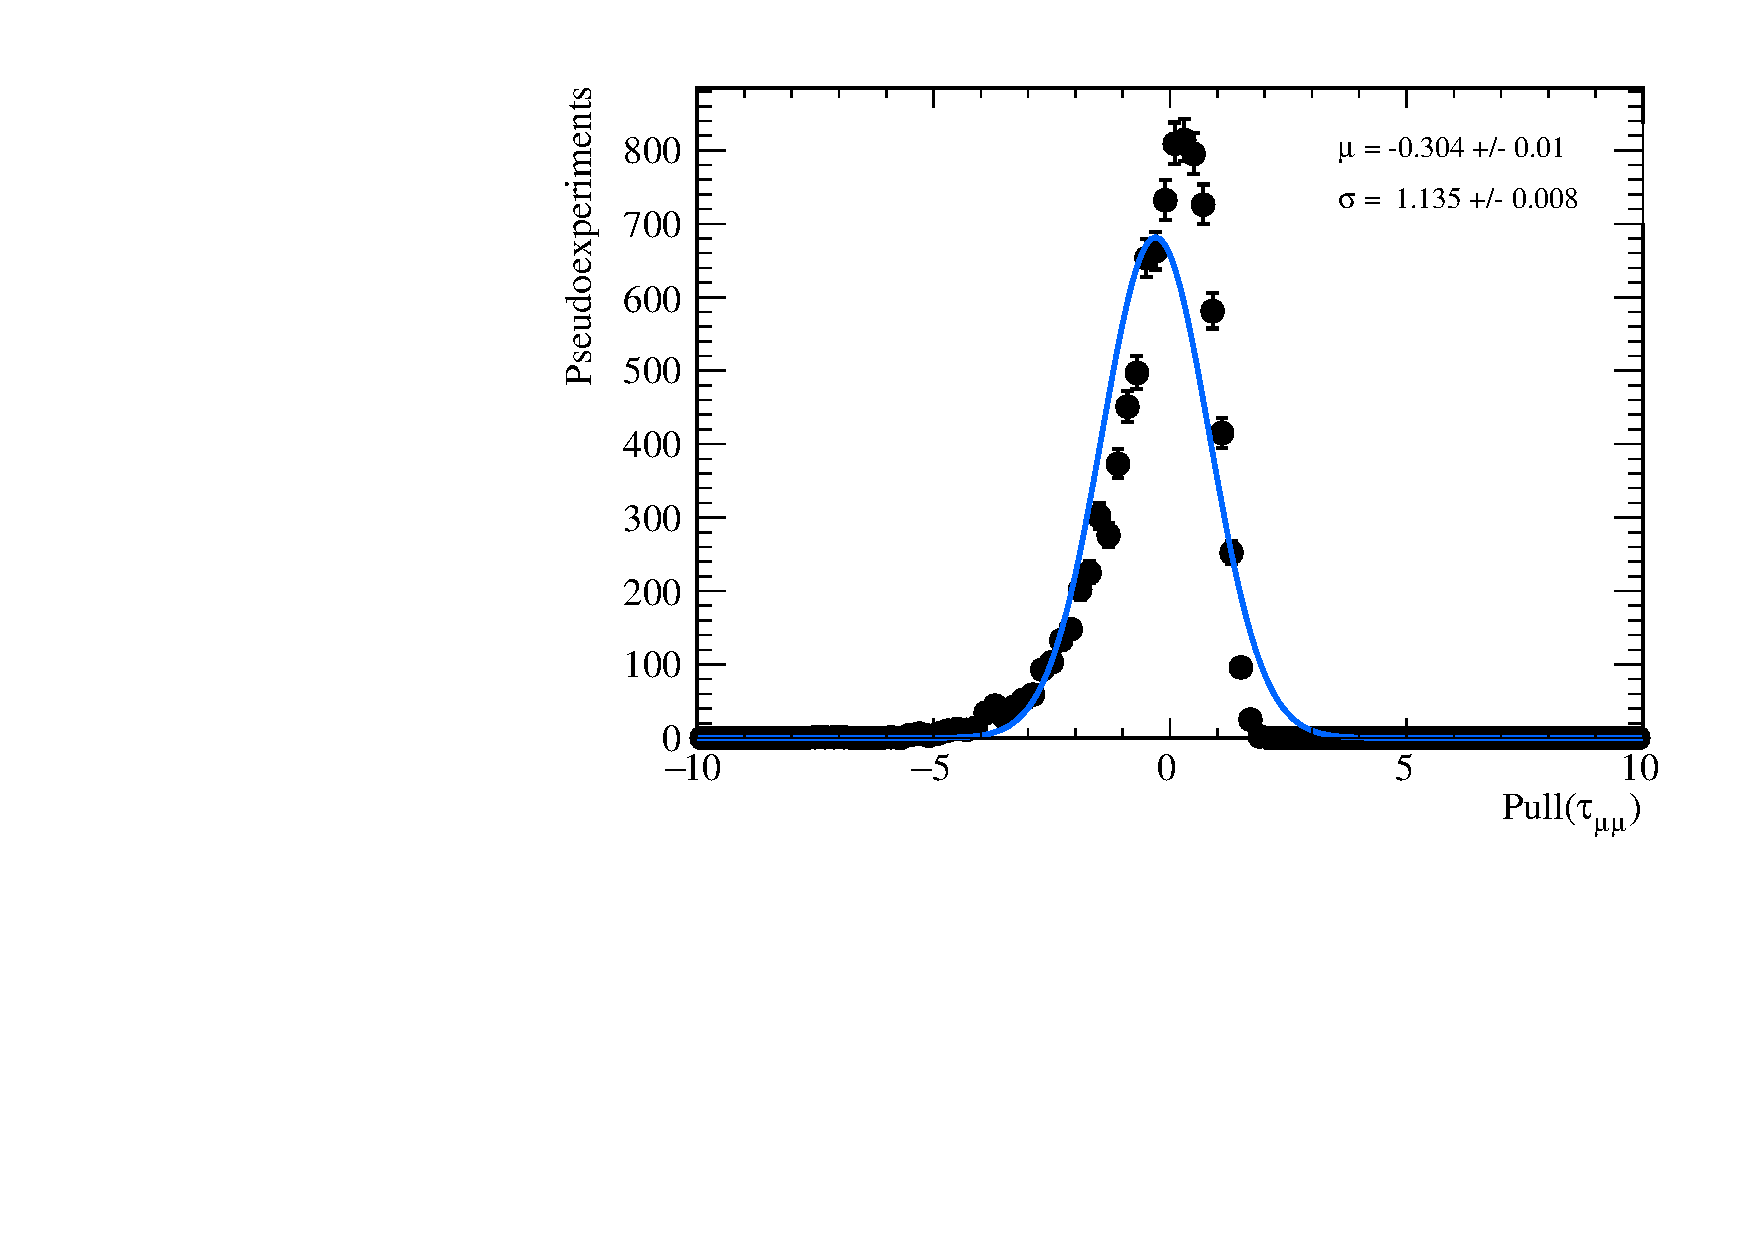
\includegraphics[width= 0.48 \textwidth]{./Figs/LifetimeMeasurement/Run1_simple_tau_pull.pdf} 
    \caption{Pull distribution (left) for \tmumu using a simplified configuration where no acceptance function is used and only signal and combinatorial background decays are generated in the mass range 4900 - 6000 \mevcc with the expected statistics for 4.4 \fb of data. Likelihood profile for \tmumu(right).}%(left) and Run 1 only (right).}
    \label{fig:taupulls}
\end{figure}

The log-likelihood profile of the  fit at a function of \tmumu reveals the cause of the biased pull distribution. For the simplified studies illustrated in Figure~\ref{fig:taupulls} the decay time is modelled by
\begin{equation}
N(t, \tau^{\mu \mu}) = N_{0}e^{-t/\tau_{\mu\mu}}.
\end{equation}
The likelihood profile as a function of decay time for this model is shown in Figure~\ref{fig:tau_ll} and there is a clear discontinuity at the zero. The discontinuity arises because the value of $N(t, \tau)$ approaches zero as $\tau$ reduces in value until at the origin when $\tau = 0$ and $N(t, \tau)$ is undefined. %jumps to infinity. The jump in value is reflected as the discontinuity in the log-likelihood profile. 
At the low statistics expected for the dataset, particularly when only Run 1 data was considered, the fitted value for \tmumu is only a few standard deviations away from this discontinuity, therefore biasing the estimation of the statistical uncertainty and changing the pull distribution from the expected Gaussian shape. However as the number of expected signal and background decays are increased the \tmumu pull distributions become Gaussian in shape as shown in Figure~\ref{fig:morestatstaupulls}. This is as expected because when the statistical uncertainty decreases, the discontinuity of Figure~\ref{fig:taupulls} is no longer within a few standard deviations of the measured \tmumu.


%\begin{figure}[htbp]
%    \centering
%        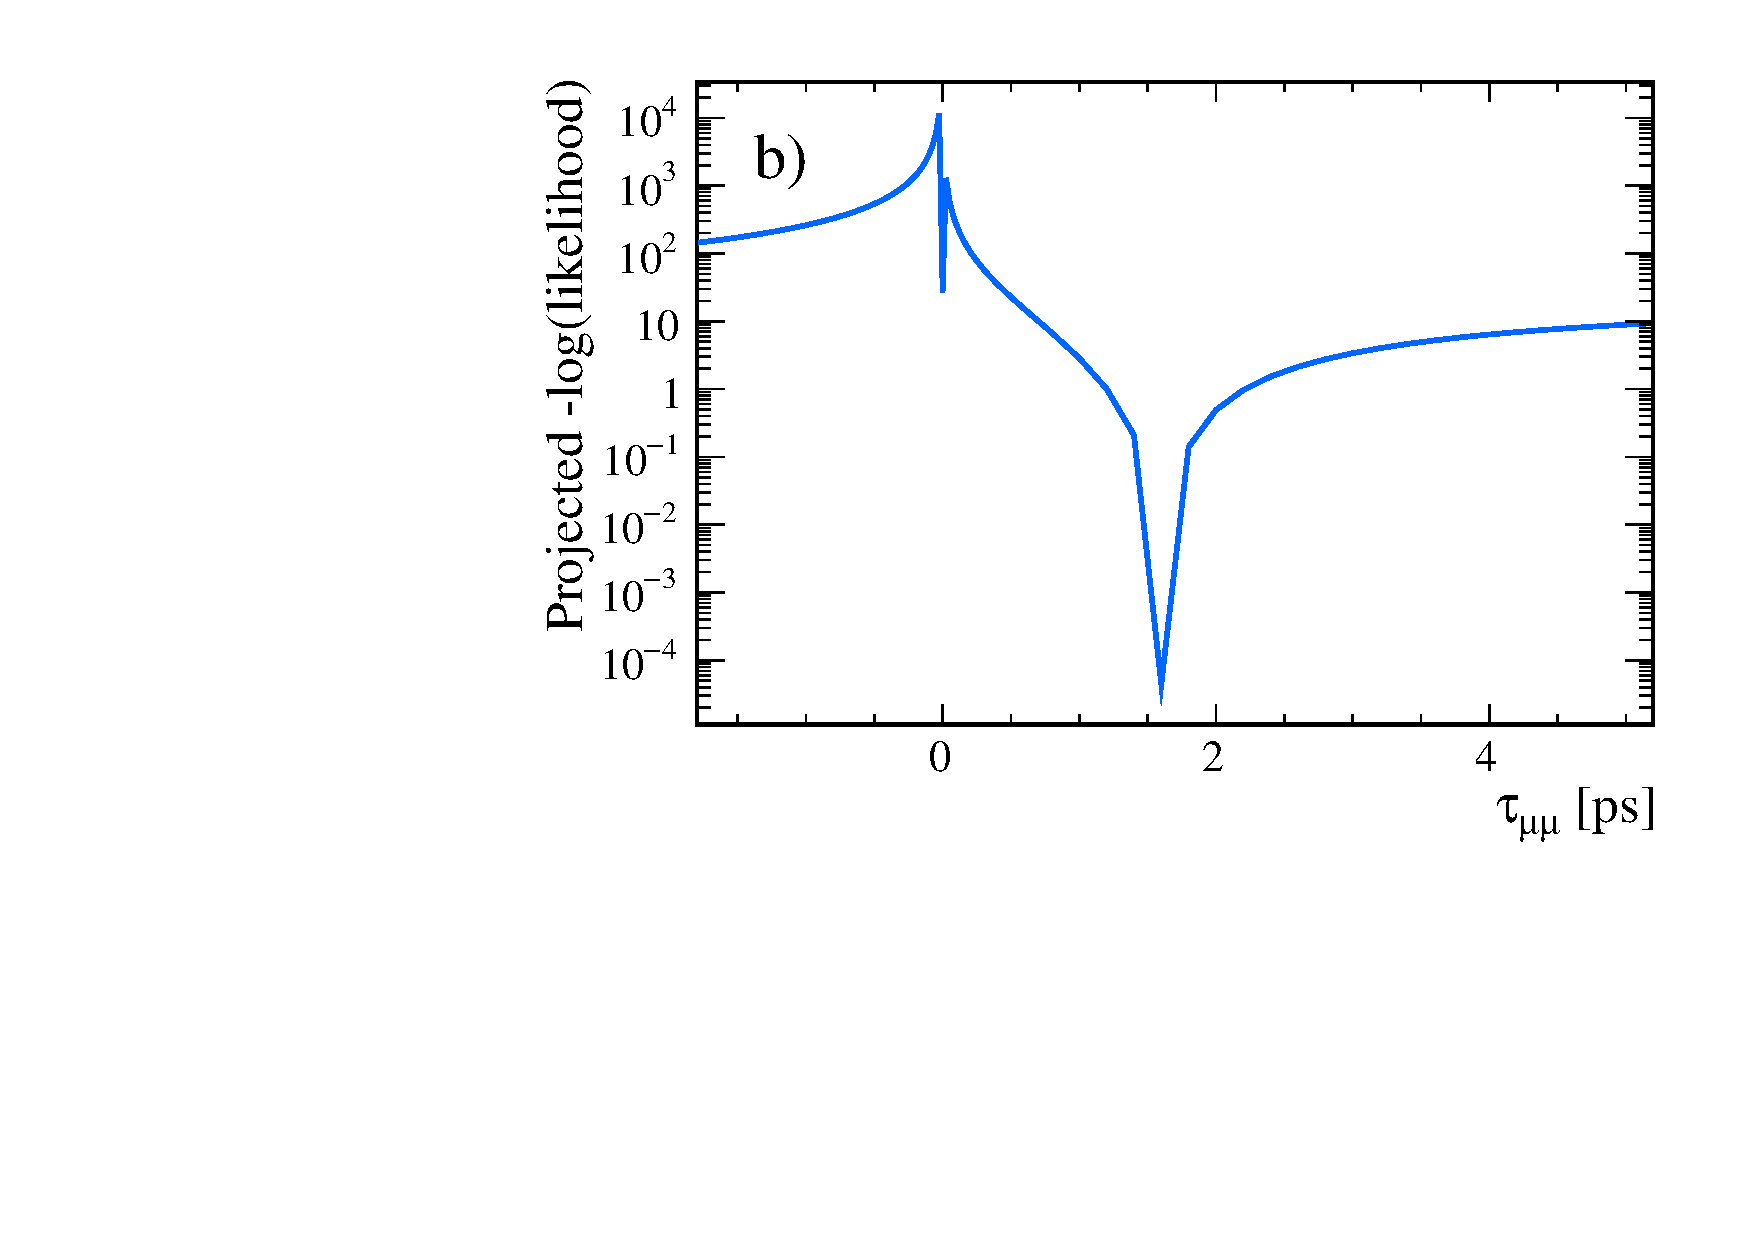
\includegraphics[width= 0.6 \textwidth]{./Figs/LifetimeMeasurement/tau_LL.pdf}  
%    \caption{Likelihood profile for \tmumu.}
%    \label{fig:taulike}
%\end{figure}

\begin{figure}[tbp]
    \centering
   \begin{subfigure}[b]{0.48\textwidth}
        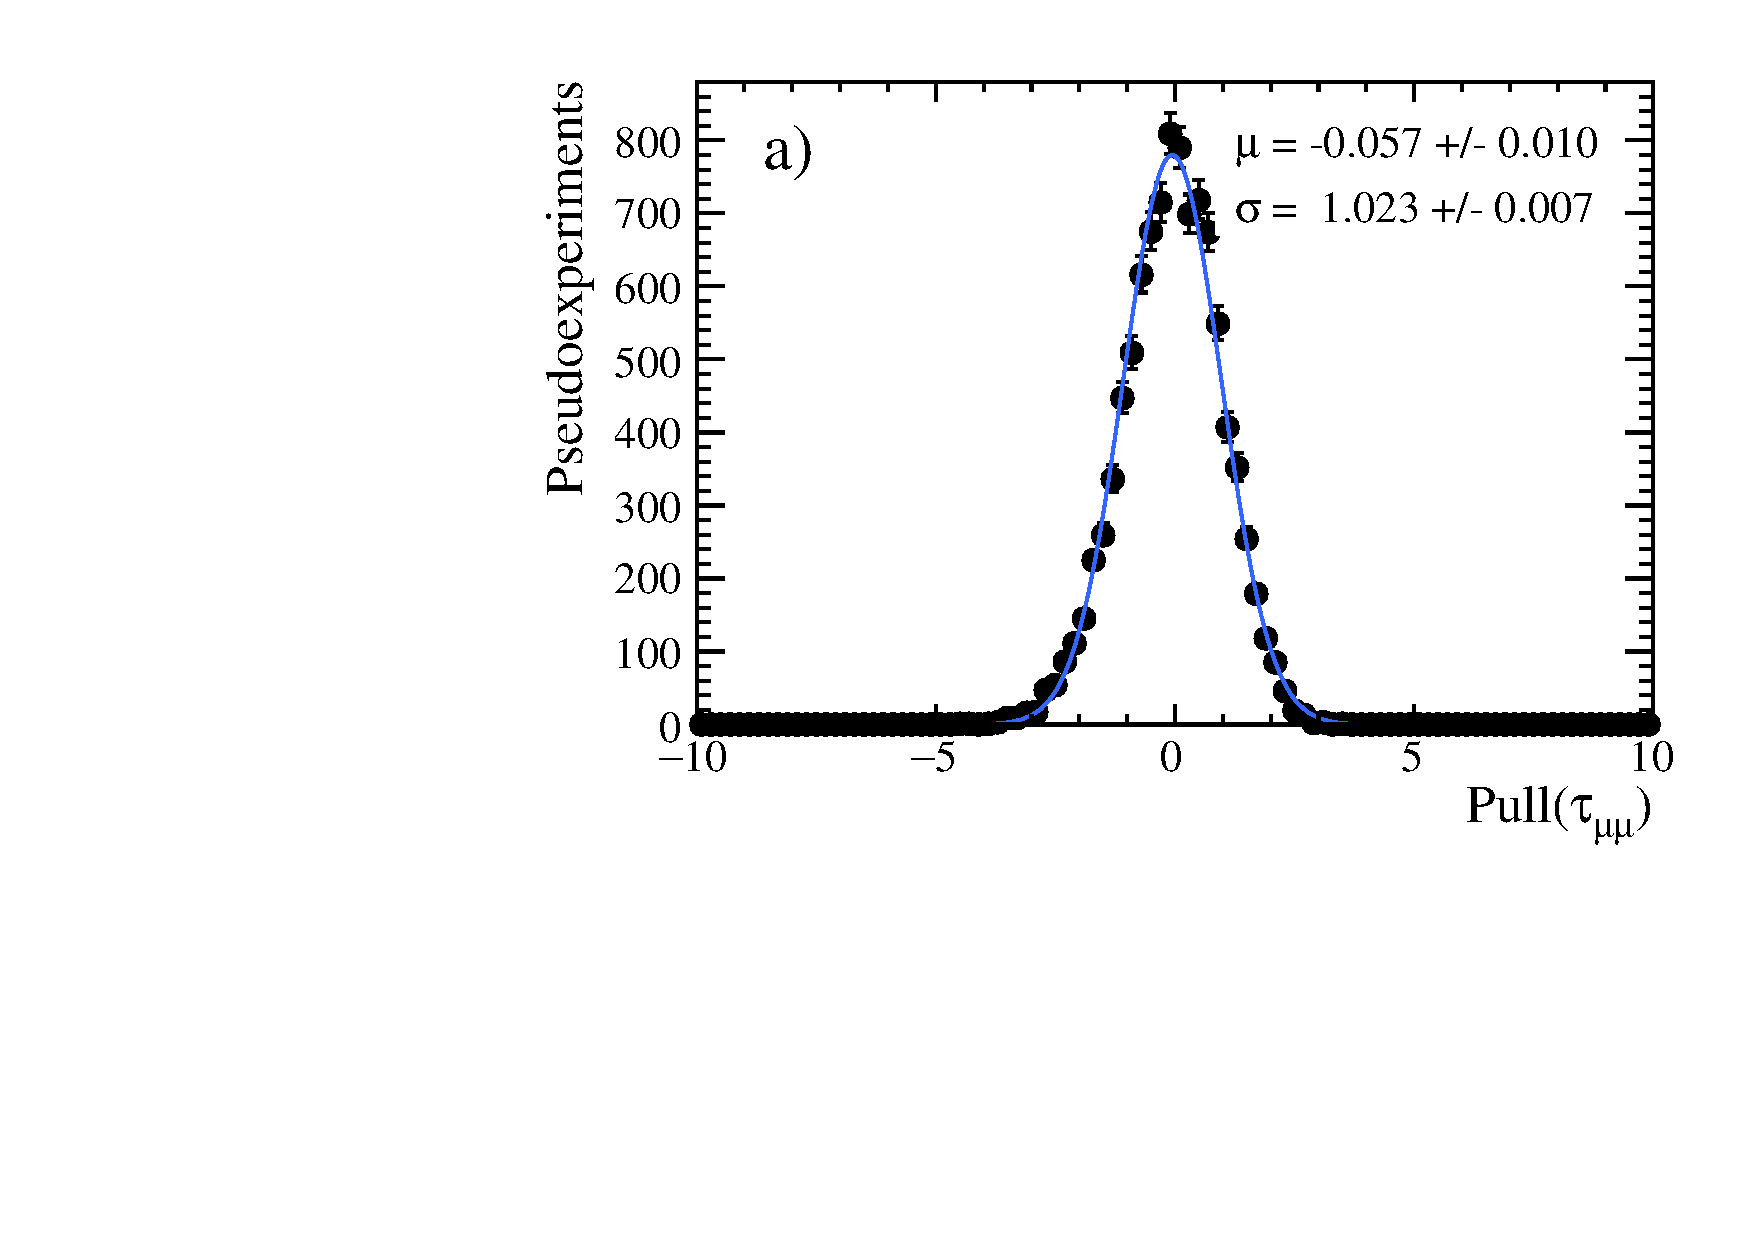
\includegraphics[width= \textwidth]{./Figs/LifetimeMeasurement/50fb_simple_tau_pull.pdf}
        %\caption{ }                                                                                                                    
        %\label{fig:BDTSsig}                                                                                                            
    \end{subfigure}
   ~ %add desired spacing between images, e. g. ~, \quad, \qquad, \hfill etc.                                                         
      %(or a blank line to force the subfigure onto a new line)                                                                         
    \begin{subfigure}[b]{0.48\textwidth}
       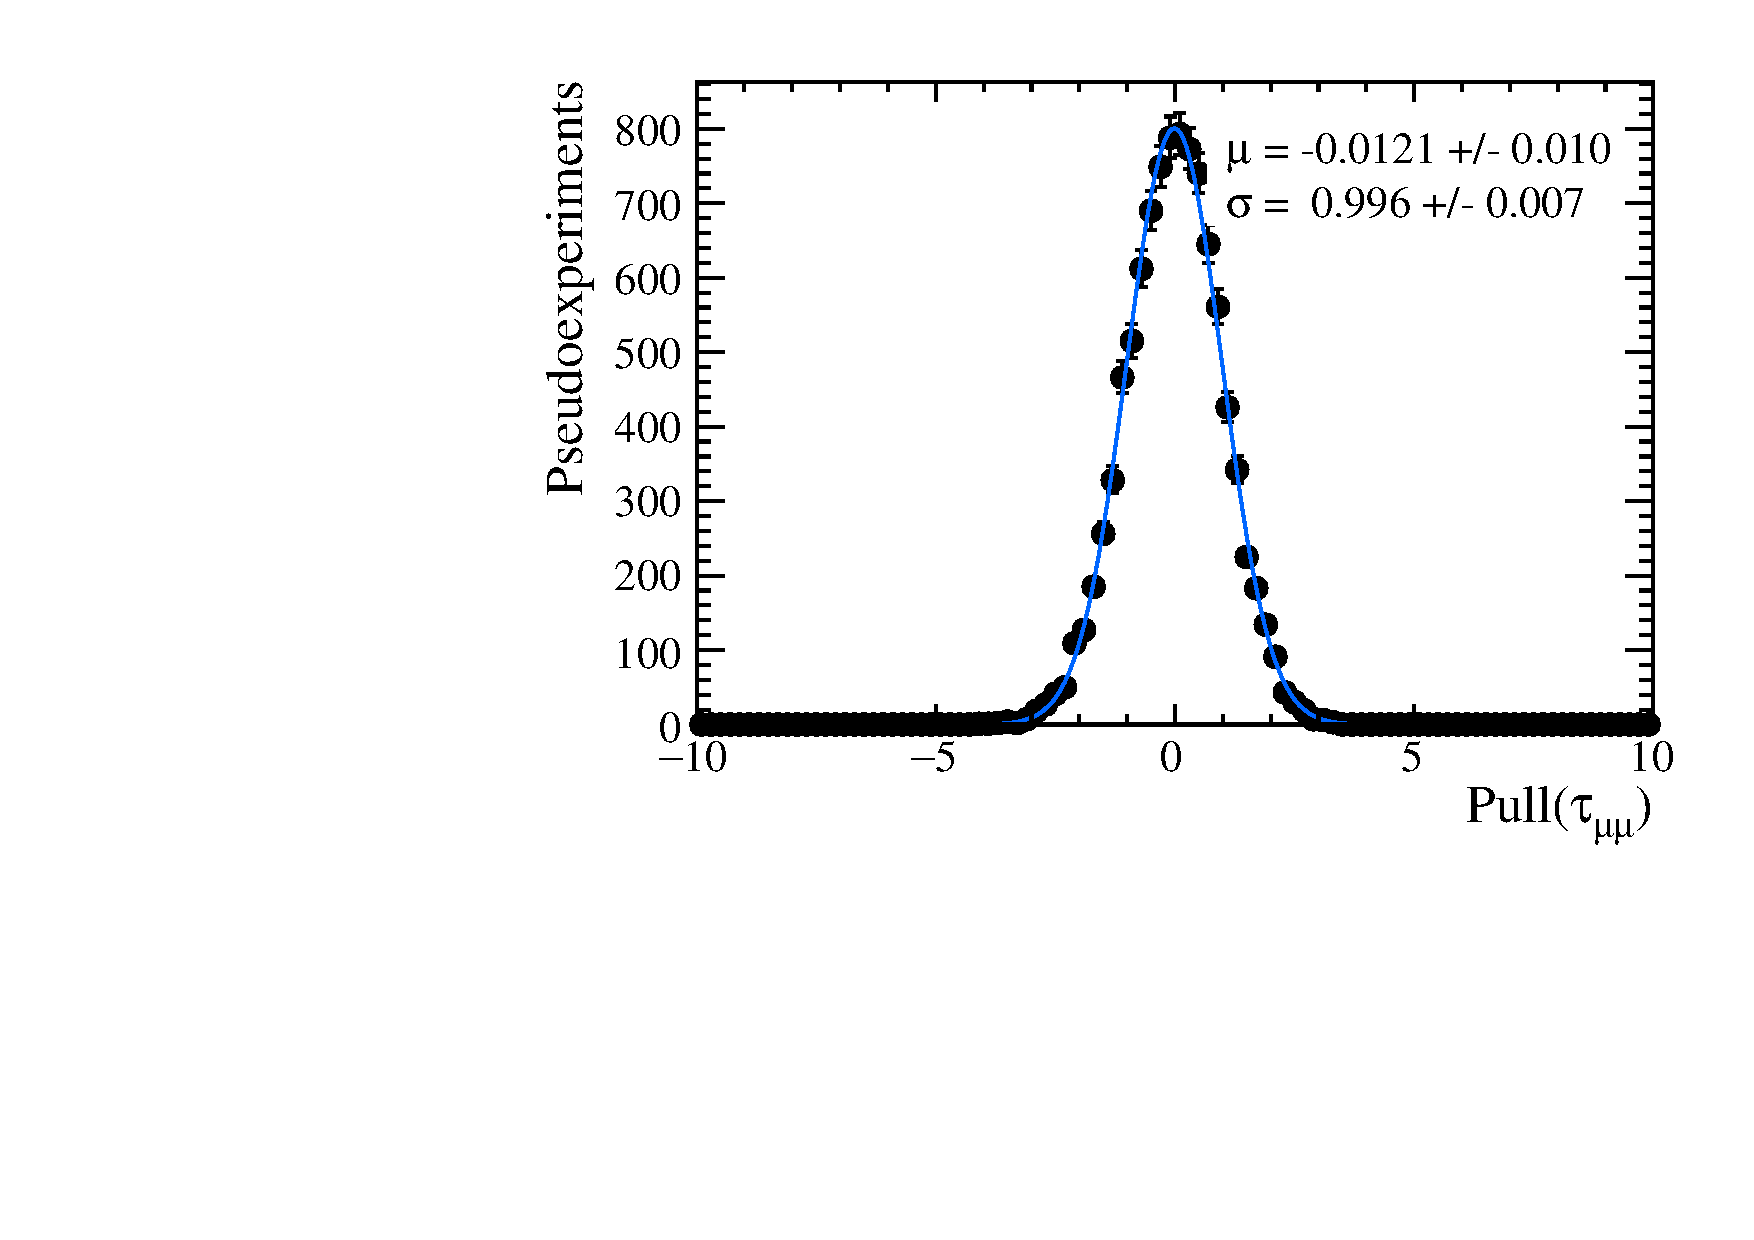
\includegraphics[width=\textwidth]{./Figs/LifetimeMeasurement/300fb_simple_tau_pull.pdf}
      %  \caption{ }                                                                                                                    
     %   \label{fig:BDTSbkg}                                                                                                            
   \end{subfigure}
    \caption{Pull distribution for \tmumu using simplified mass and decay time model for 50~\fb (left) and 300~\fb (right) where no acceptance function is used and only signal and combinatorial background decays are generated in the mass range 4900 - 6000 \mevcc.}
    \label{fig:morestatstaupulls}
\end{figure}


The bias in the \tmumu pull distribution shows that the distribution cannot be interpreted in the usual way and also that the statistical uncertainties from the \ml to the weighted decay time distribution may not be correct. 

Another way to assess the accuracy of the statistical uncertainties returned by the \ml fit is the coverage of the uncertainties; the percentage of fitted \tmumu values from the pseudoexperiments that fall within 1, 2 and 3 standard deviations of the lifetime used as the input value. Table~\ref{tab:LifetimeCoverage} shows the coverage of the statistical uncertainties for \tmumu for a set of 10,000 pseudoexperiments for the expected \bsmumu and combinatorial background yields with 4.4~\fb alongside the intervals expected for a Gaussian distribution. The simple toy configuration used to produce the log-likelihood function is used. A comparison between the coverage of \tmumu and the Gaussian intervals shows that the coverage of the statistical uncertainties is very close to the expected values.

\begin{table}[ht]
\begin{center}
\begin{tabular}{lccc}
\toprule \toprule
 & \tmumu &   \Gmumu$\equiv \frac{1}{t_{\mu\mu}}$  &Gaussian \\ \midrule 
$1\sigma$ & 68.50 $\pm$ 0.08$\%$ & 67.92 $\pm$ 0.08$\%$ & 68.27$\%$ \\
$2\sigma$ &  93.44$\pm$ 0.10$\%$ & 95.91$\pm$ 0.10$\%$ &  95.45$\%$ \\
$3\sigma$ & 98.06$\pm$ 0.10$\%$ &  99.55$\pm$ 0.10$\%$ & 99.73$\%$ \\ \bottomrule \bottomrule
\end{tabular}
\vspace{0.7cm}                                                                                                                                               
\caption{Coverage of the statistical uncertainties evaluated as the number of pseudoexperiments for the expected number of decays with measured \tmumu (\Gmumu) values that are with 1, 2 and 3 times $\sigma_{\tau_{\mu\mu}}$ ($\sigma_{\Gamma_{\mu\mu}}$) of the generated lifetime value.}
\label{tab:LifetimeCoverage}
\end{center}
\vspace{-1.0cm}                                                                                                                                               
\end{table}

Alternatively, a biased pull distribution can be avioded by fitting for the inverse of the effective lifetime, \invtmumu$ \equiv$ \Gmumu. The pull distributions for \Gmumu are shown in Figure~\ref{fig:gammapulls} and produce unbiased pull values regardless of the amount of data. This is unsurprising given the smooth log-likelihood profile as a function of \Gmumu also shown in Figure~\ref{fig:gammapulls}. Furthermore the statistical coverage of \Gmumu is closer to the expected Gaussian coverage than the coverage of \tmumu.  %However the lifetime is a more interesting variable from a physics point of view due to its relationship with \ADG. %Furthermore fitting for the \Gmumu introduces a different type of bias in to the fit, but this is negligible for the expected number of statistics. 


Ideally, the fit strategy would be performed to extract the lifetime not the inverse lifetime, however for the moment the \ml fit for both \tmumu and \Gmumu are used in the toy studies. The statistical coverage for both parameters is good and using either is reasonable. The final decision was made based on the statistical coverage for the observed number of decays in the data set. 


%\begin{figure}[htbp]
%    \centering
%        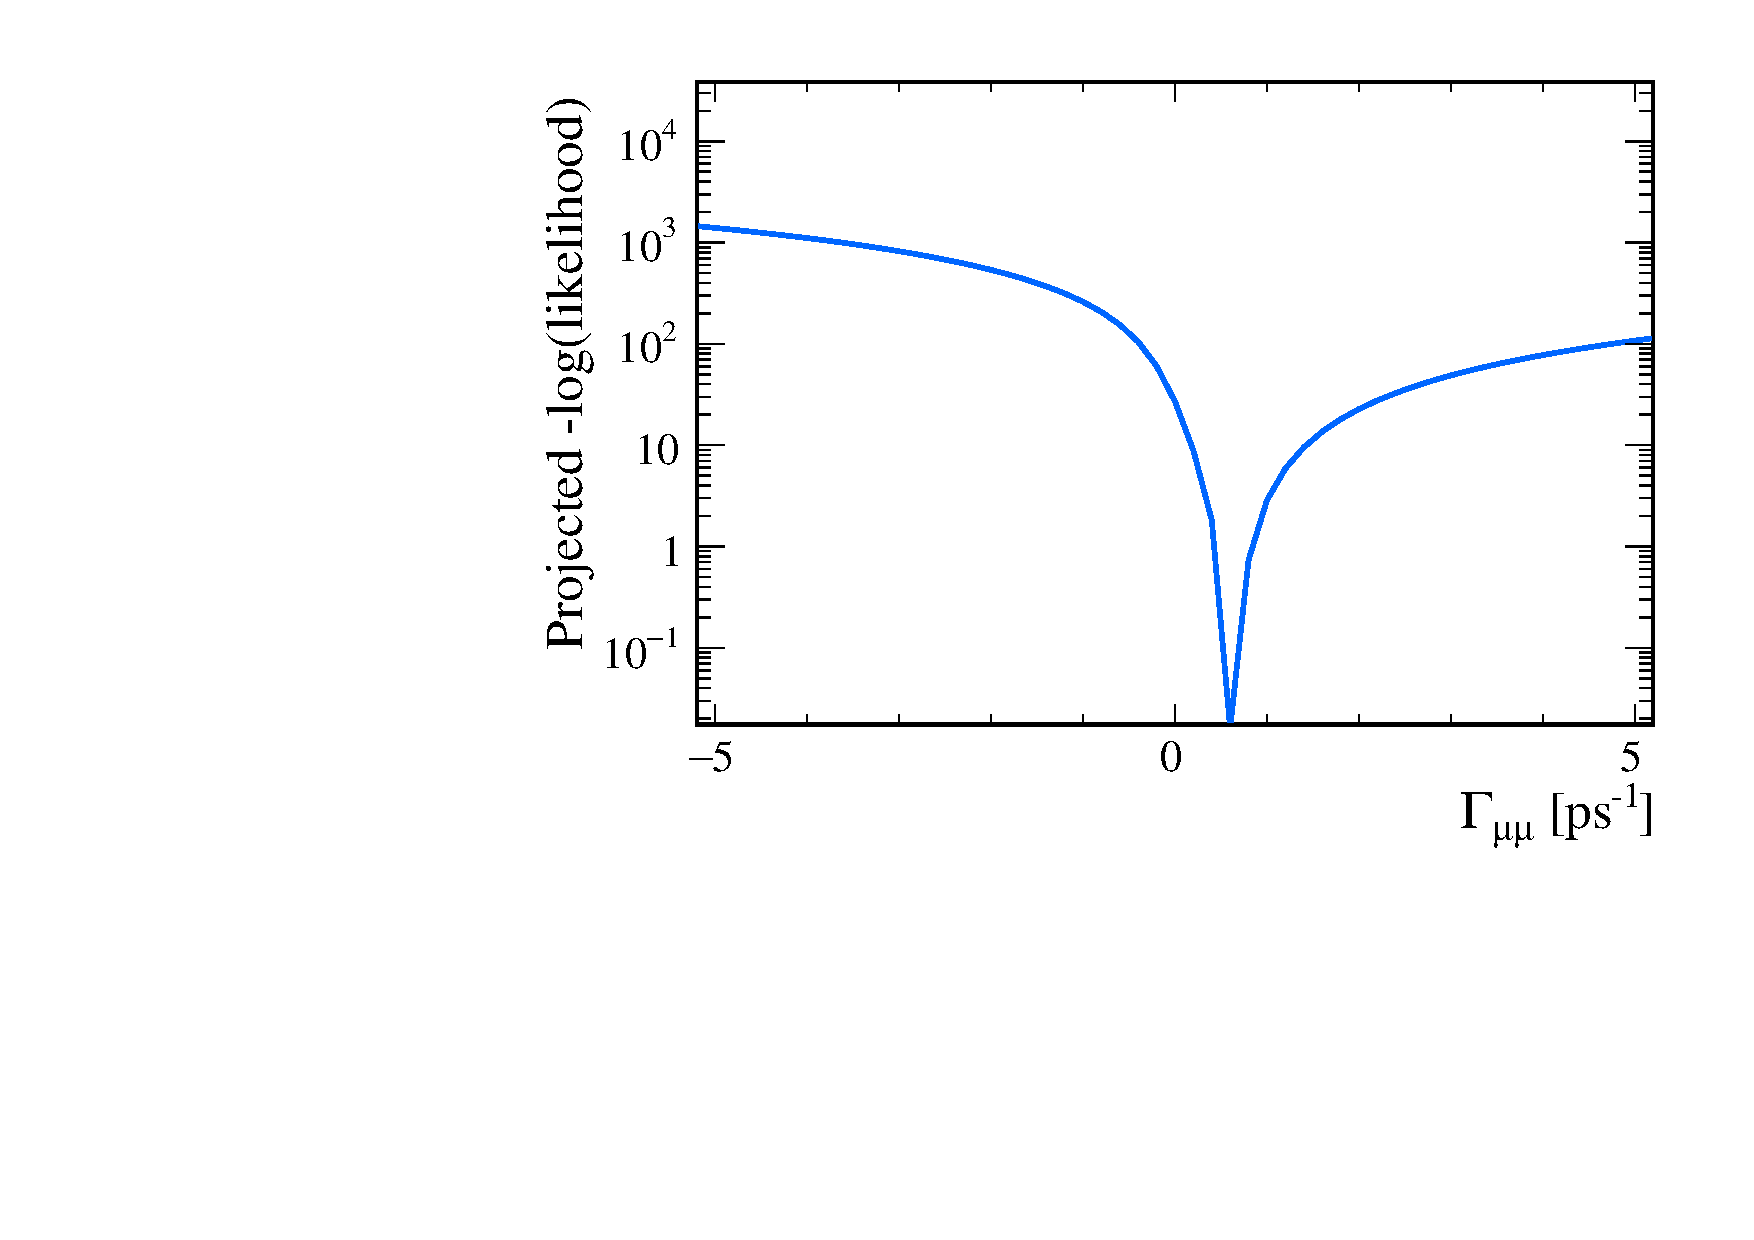
\includegraphics[width= 0.49 \textwidth]{./Figs/LifetimeMeasurement/Gamma_LL.pdf}  
%    \caption{Likelihood profile for \Gmumu.}
%    \label{fig:gammalike}
%\end{figure}

\begin{figure}[tbp]
    \centering
     %   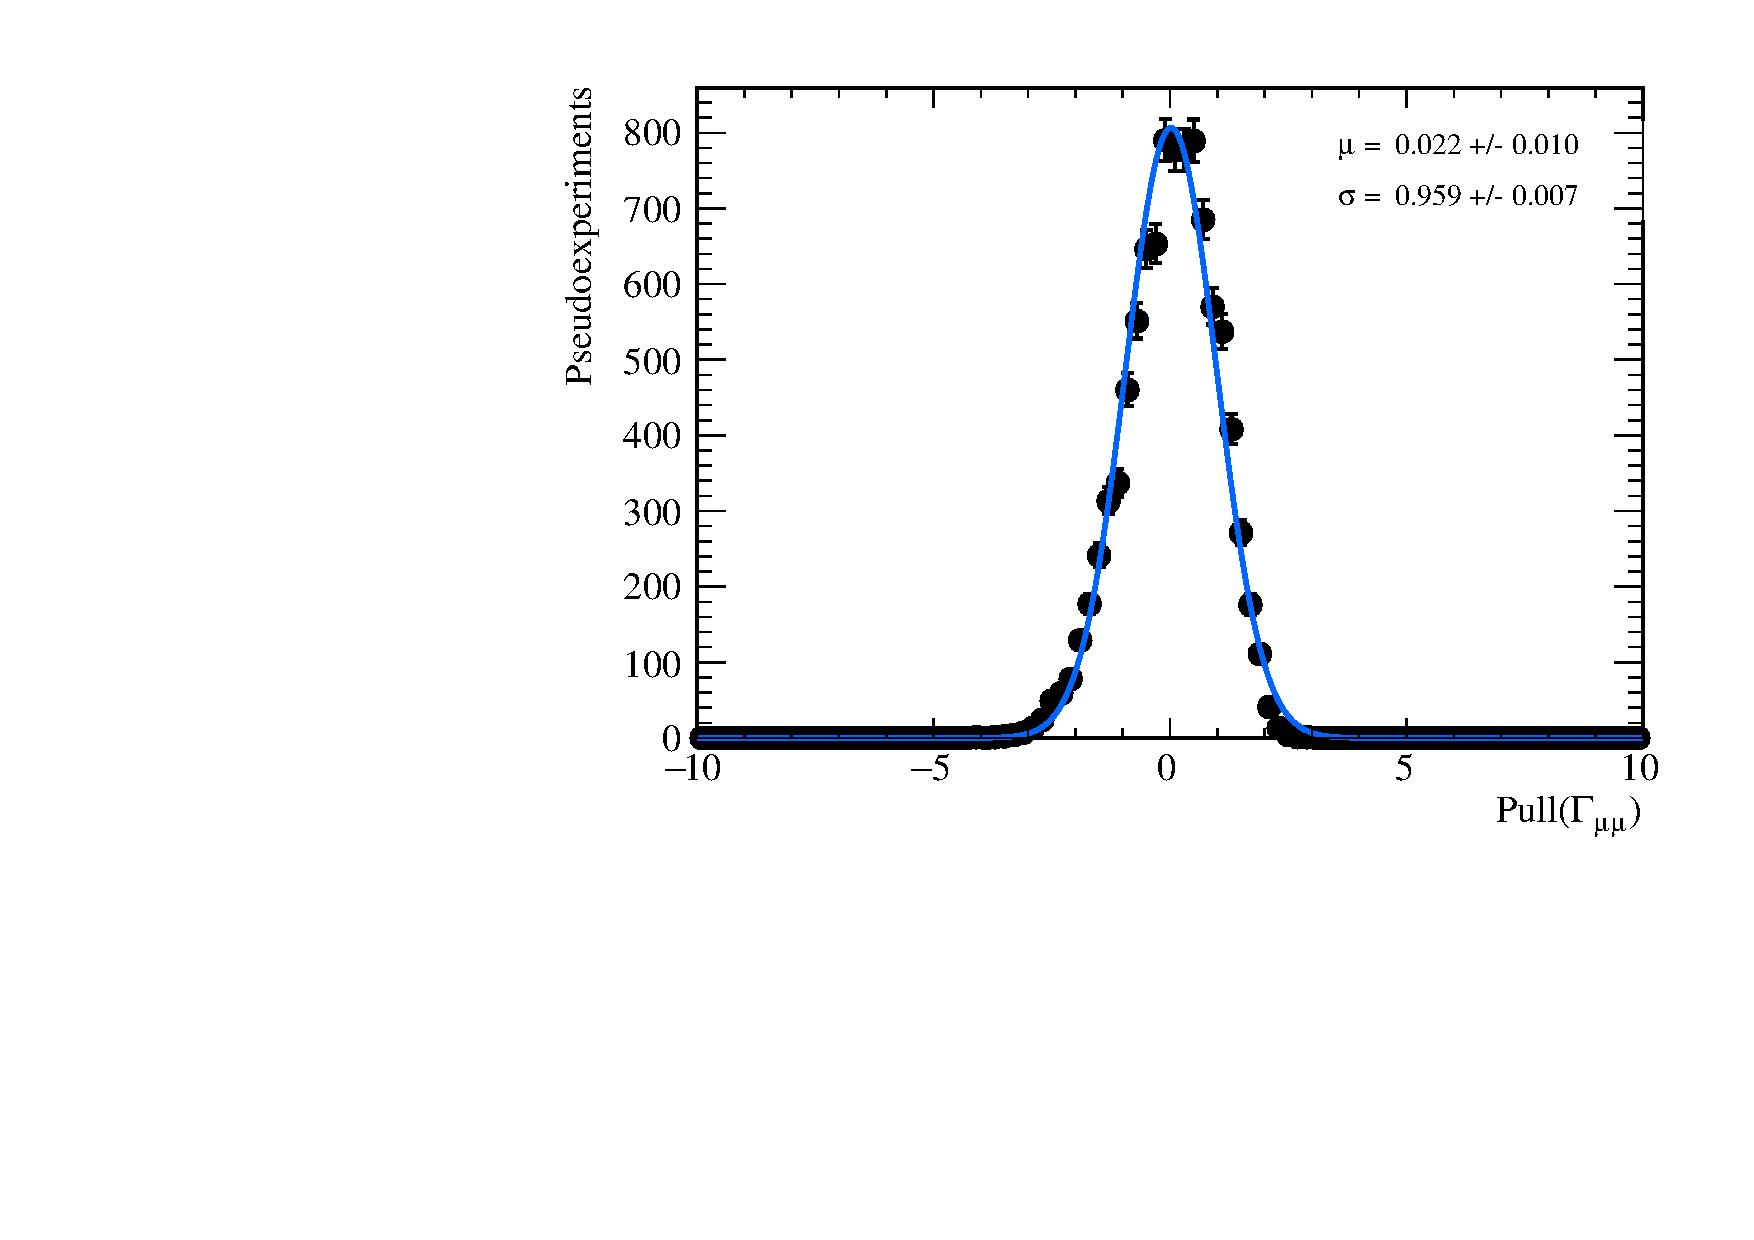
\includegraphics[width= 0.49 \textwidth]{./Figs/LifetimeMeasurement/Run1_simple_gamma_pull.pdf}
       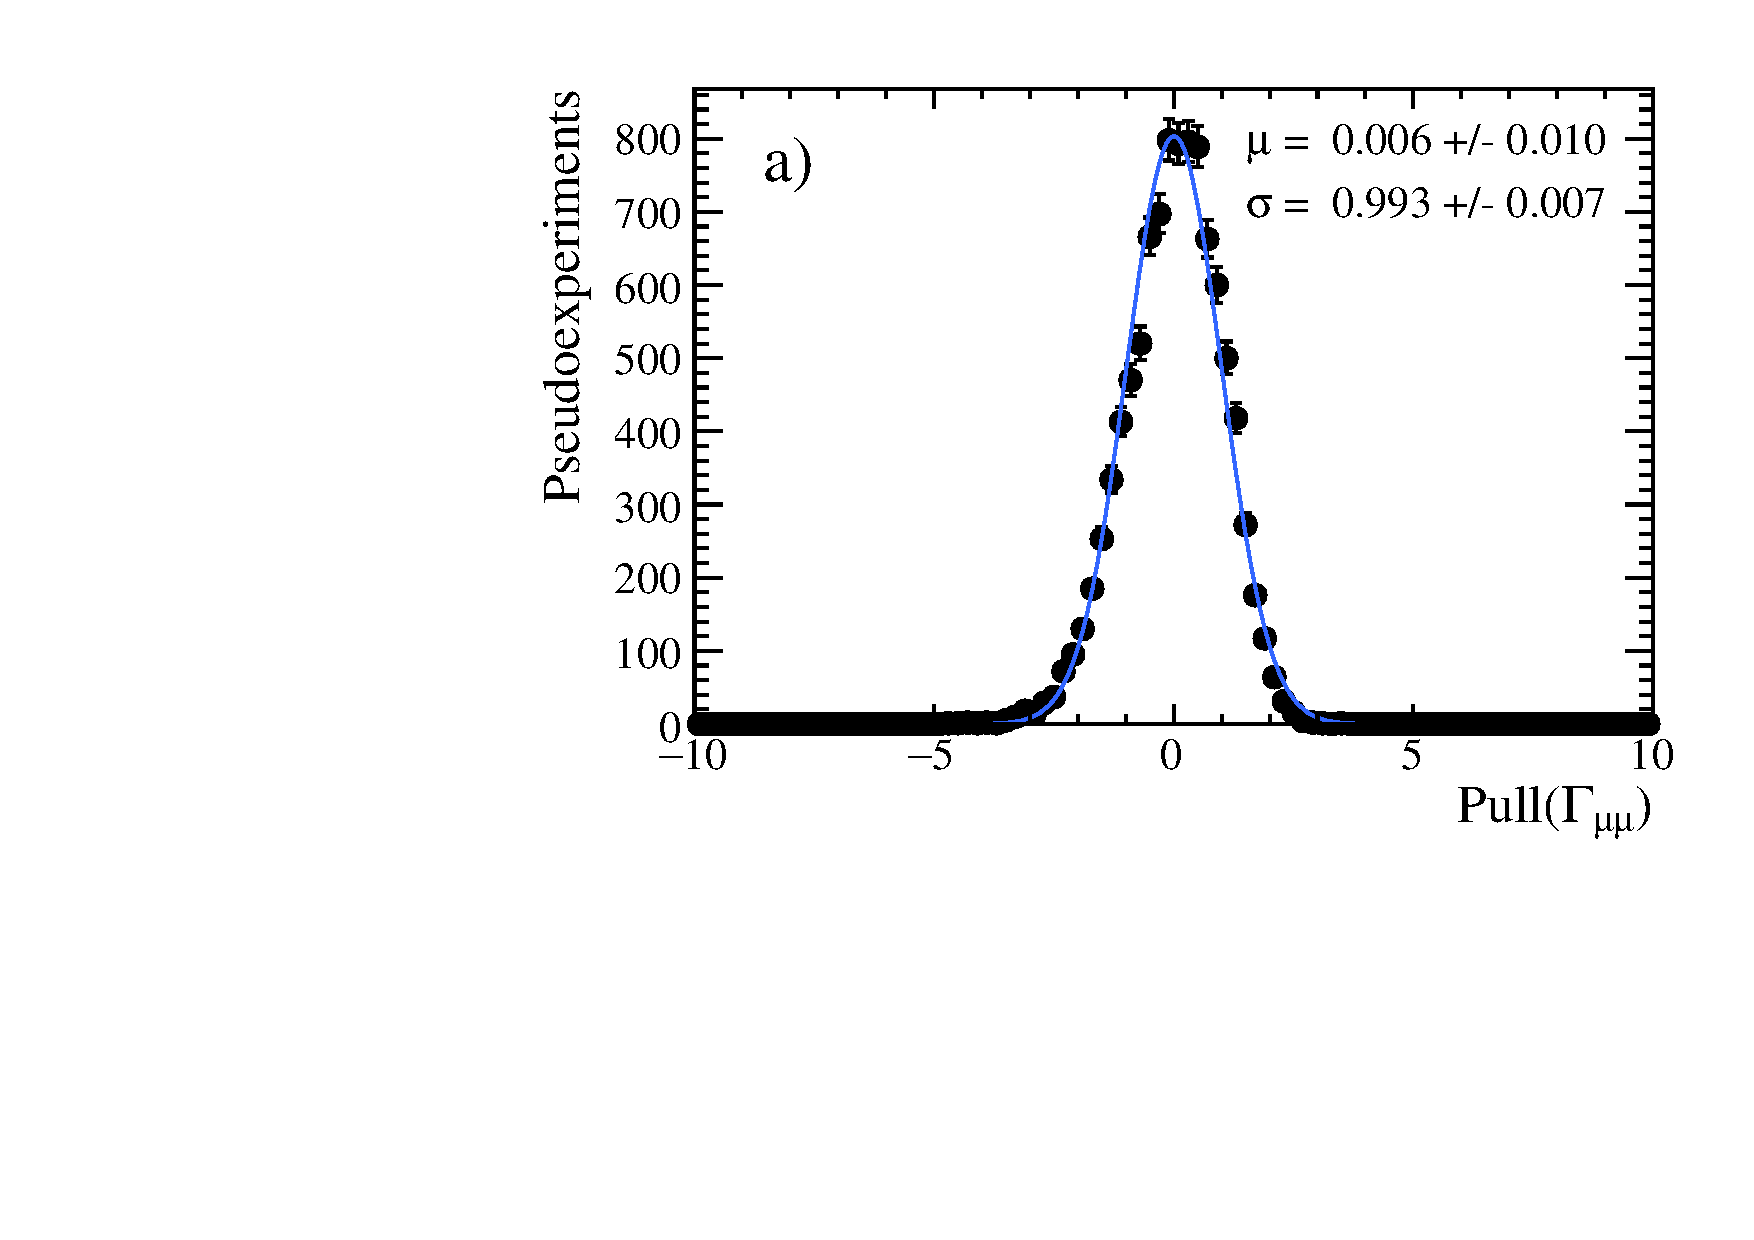
\includegraphics[width=0.49 \textwidth]{./Figs/LifetimeMeasurement/CKM_simple_gamma_pull.pdf}
     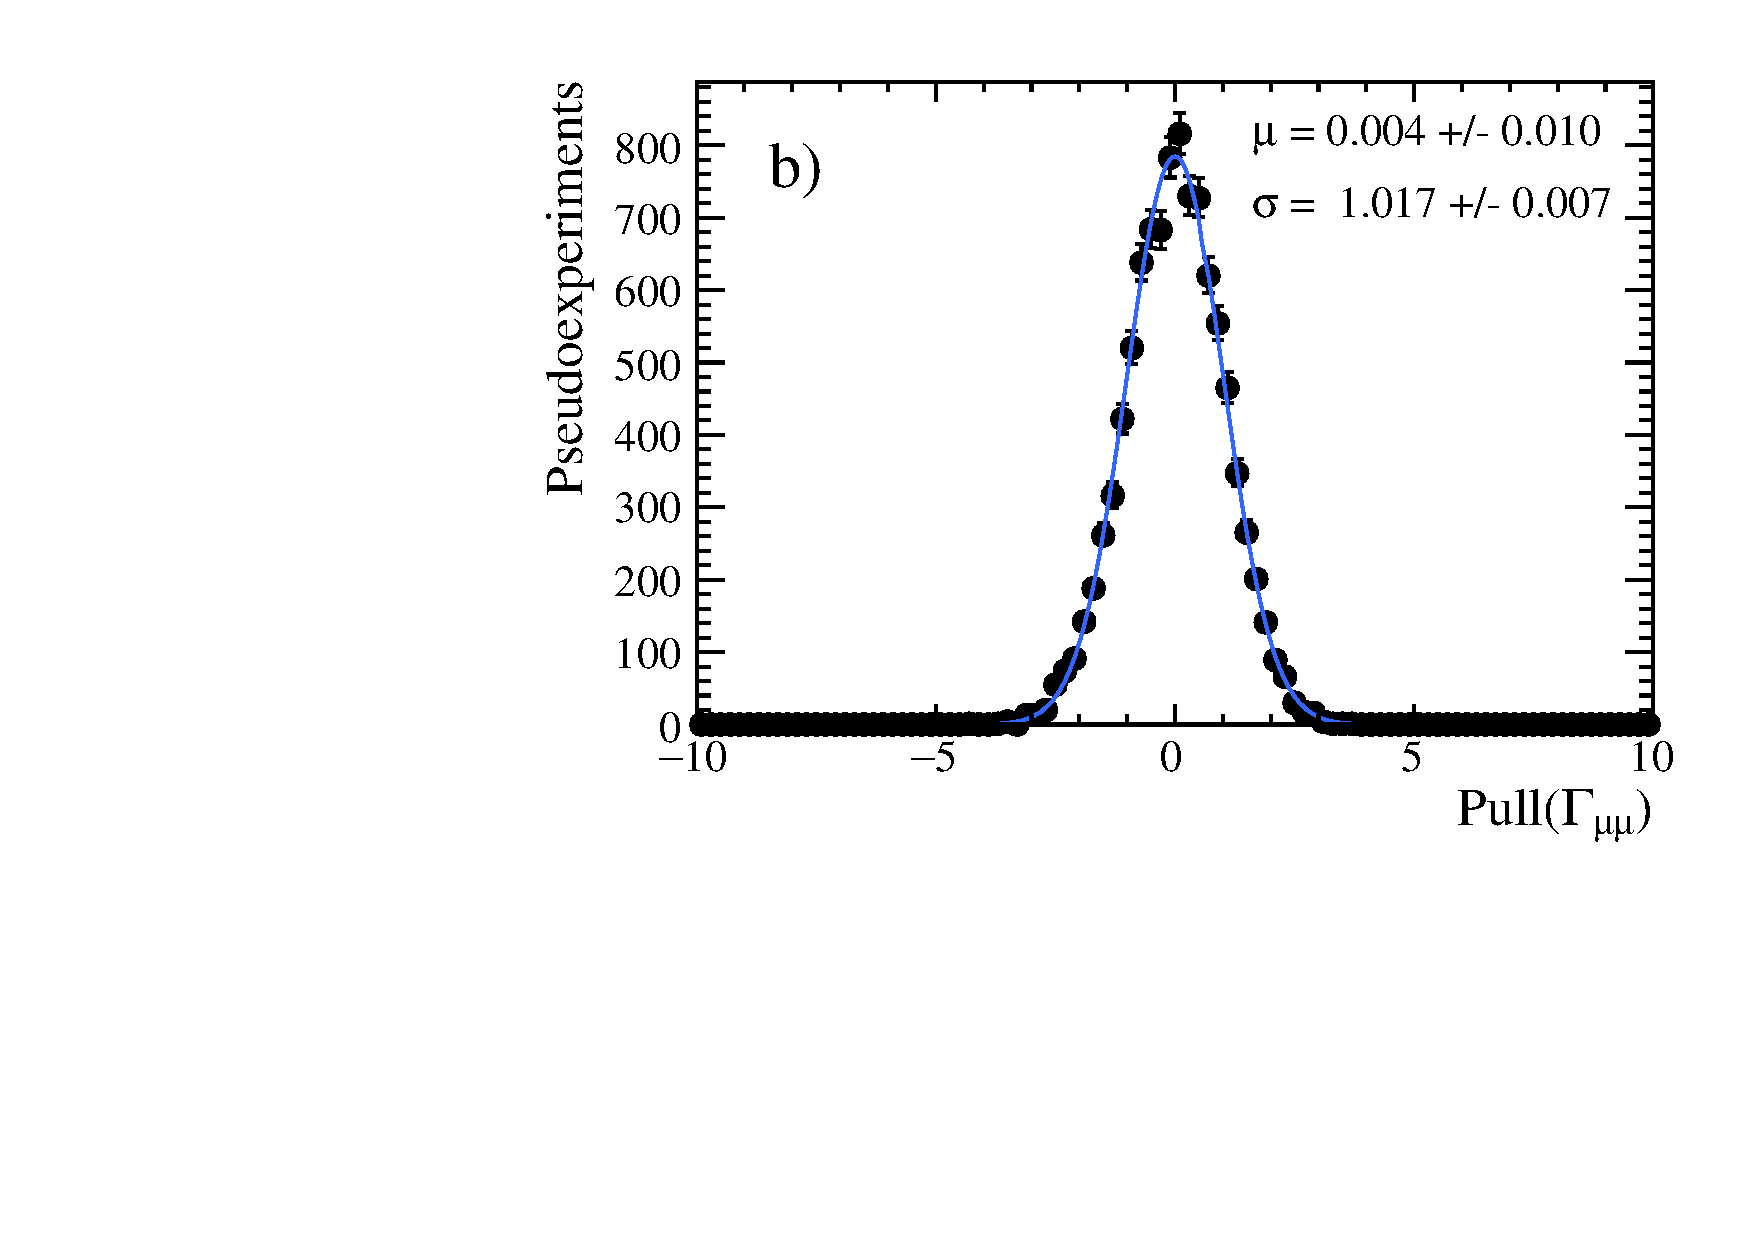
\includegraphics[width= 0.49 \textwidth]{./Figs/LifetimeMeasurement/50fb_gamma_pull.pdf}
      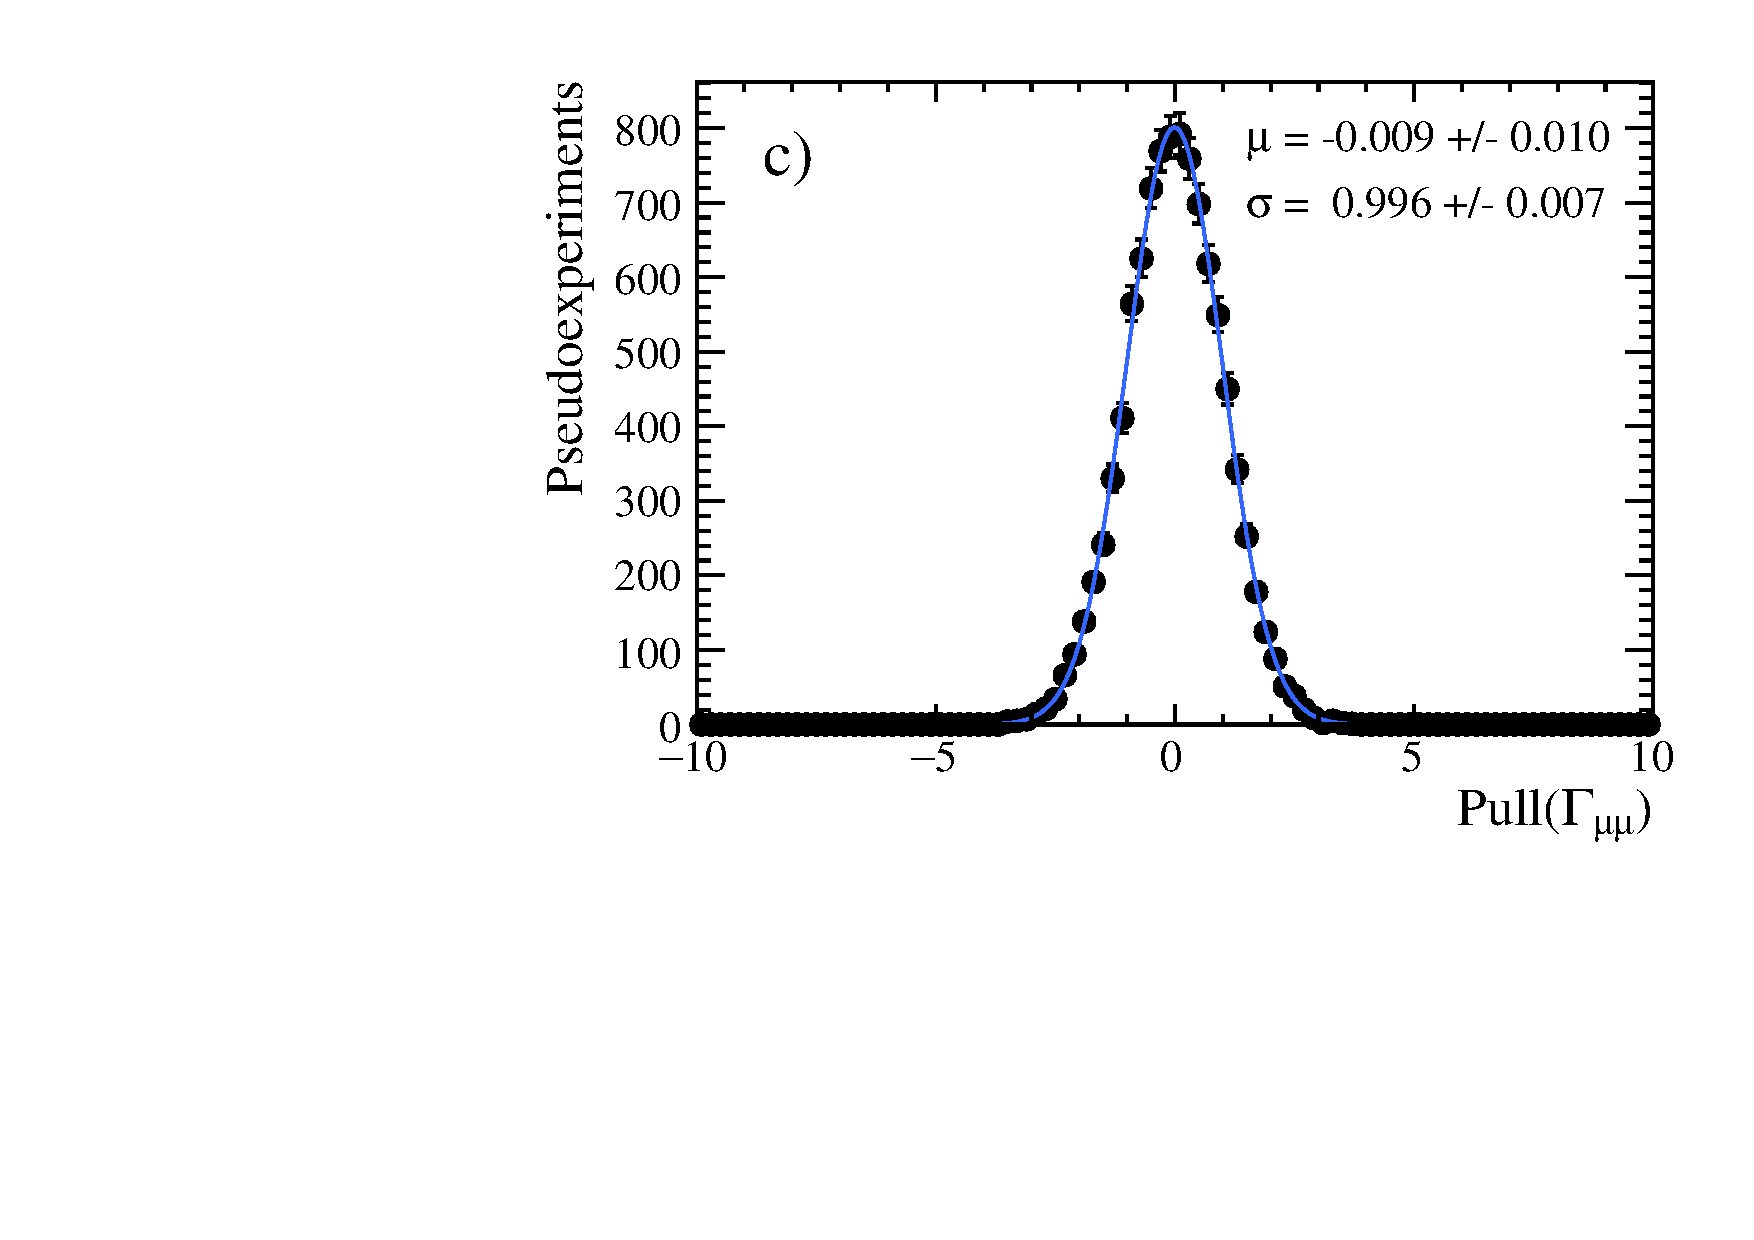
\includegraphics[width=0.49 \textwidth]{./Figs/LifetimeMeasurement/300fb_simple_gamma_pull.pdf}
        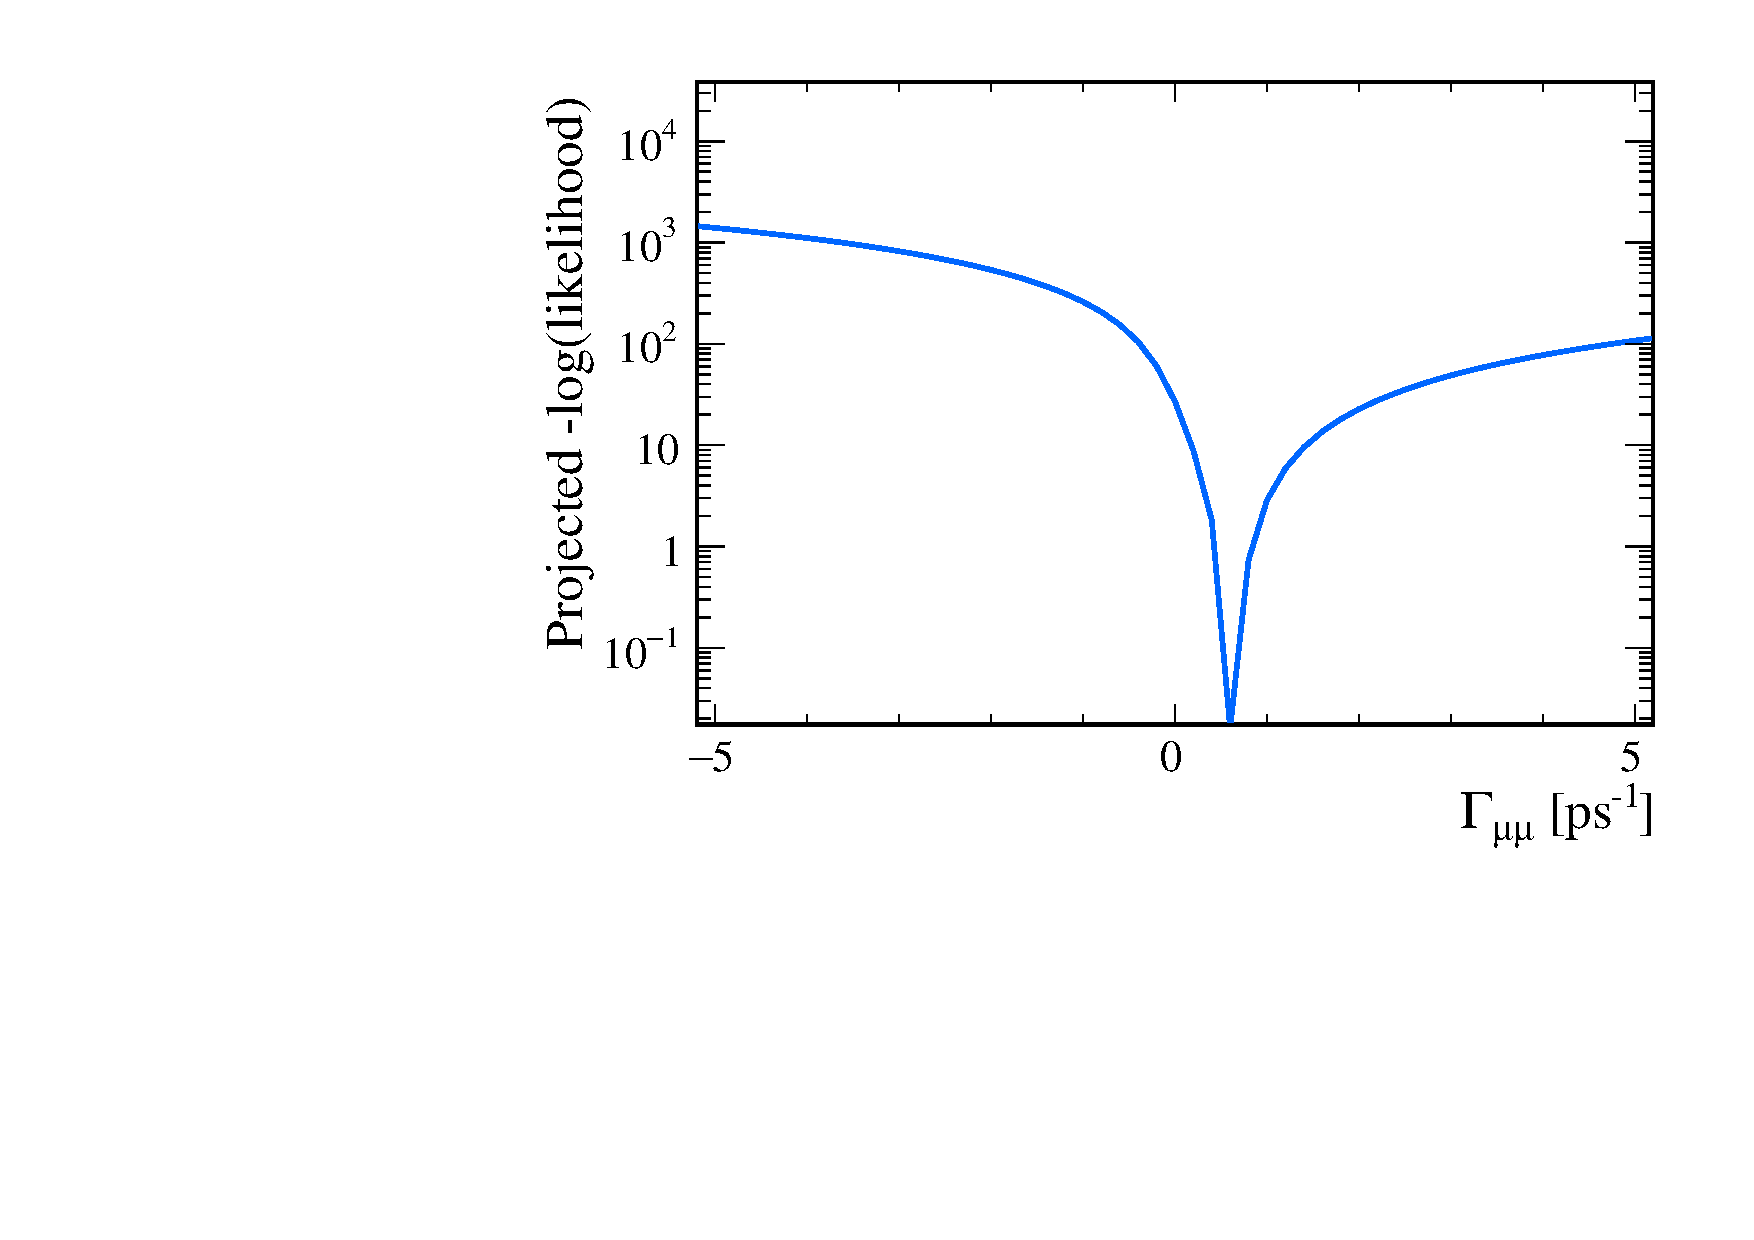
\includegraphics[width= 0.49 \textwidth]{./Figs/LifetimeMeasurement/Gamma_LL.pdf}  

  \caption{Pull distribution for \Gmumu using simplified toy studies for 4.4 (top left), 50 (top right) and 300 (bottom left) \fb and the likelihood profile as a function of \Gmumu (bottom right).}
    \label{fig:gammapulls}
\end{figure}




\subsection{Optimisation results}
\label{sec:toyresults}

The mass distribution of the expected number of \bsmumu candidates passing the effective lifetime selection is shown in Figure~\ref{fig:toygen} alongside the corresponding decay time distribution for one pseudoexperiment for 4.4~\fb of Run~1 and Run~2 data. 
The contributions from the different signal and background sources are shown and the backgrounds beneath the \bs mass peak are the combinatorial background and the tails of the \bhh, \bdmum and \lambdab backgrounds. The expected mass distribution is used to determine a range of mass fit configurations to be tested using toy studies to find the configuration that produces the smallest expected uncertainty on the measurement of \tmumu and \Gmumu.


%In each fit configuration the mass \pdf has the form
%\begin{equation}
%P(m) = N_{sig}P_{sig}(m) + \displaystyle\sum_{i} N_{bkg}^{i}P_{bkg}^{i}(m)
%\end{equation}
%where $N_{sig(bkg)}$ and $P(m)_{sig(bkg)}$ are the yields and \pdfs of the signal (backgrounds) in the fit. 

In each mass fit configuration the mass \pdf in Equation~\ref{eq:masspdf} is used and the mass ranges and backgrounds included in the \pdf for the different configurations are given in Table~\ref{tab:toyconfig}.


For each possible mass fit configuration the \bsmumu, \bdmumu and combinatorial background yields are left free in the fit whereas the yields of any other backgrounds are constrained to their expected values. The mass shapes of all components are fixed in the \ml fit except the slope of the combinatorial background because this is not accurately known in data. 
The SM predicts that \tmumu is equal to the lifetime of the heavy \bs mass eigenstate, \tH, the average value calculated by the Particle Data Group is used to generated events for the pseudoexperiments~\cite{Olive:2016xmw}. %Standard Model prediction, \tmumu = \tH, for the \bsmumu effective lifetime is used to generate events for the pseudoexperiments where \tH is taken from the PDG value. 
Also, regardless of which background components are included in the mass fit all backgrounds are generated for each mass range. %The \pdfs used in the pseudoexperiments are detailed in Appendix~\ref{}.

A total of 10,000 pseudoexperiments are performed for each mass configuration and the results are given in Table~\ref{tab:toyResults}. The mean and widths of \Gmumu, the \bsmumu yield and combinatorial background yield and slope as well as the median expected uncertainty on \tmumu and \Gmumu are used to measure the performance of each mass fit configuration. The pull distribution of the fit for \tmumu is not used to assess the performance of each mass fit configuration given the discussion in Section~\ref{sec:tauORinvtau}.



The expected statistical uncertainties for \tmumu and \Gmumu are smallest for fit configuration 11, where the mass range is restricted to 5320 - 6000 \mevcc and only the \bsmumu and combinatorial background components are used in the total mass \pdf. The mean and widths for the different pull distributions are consistent with the expected mean of 0 and width of 1 for this fit configuration. The larger mass ranges with more background components included in the mass \pdf have larger expected uncertainties for \tmumu and \Gmumu as well as clearly biased pull distributions. %It is not surprising that the simplest fit performs the best given the very low expected number of events. 

\begin{figure}[hp]
    \centering
        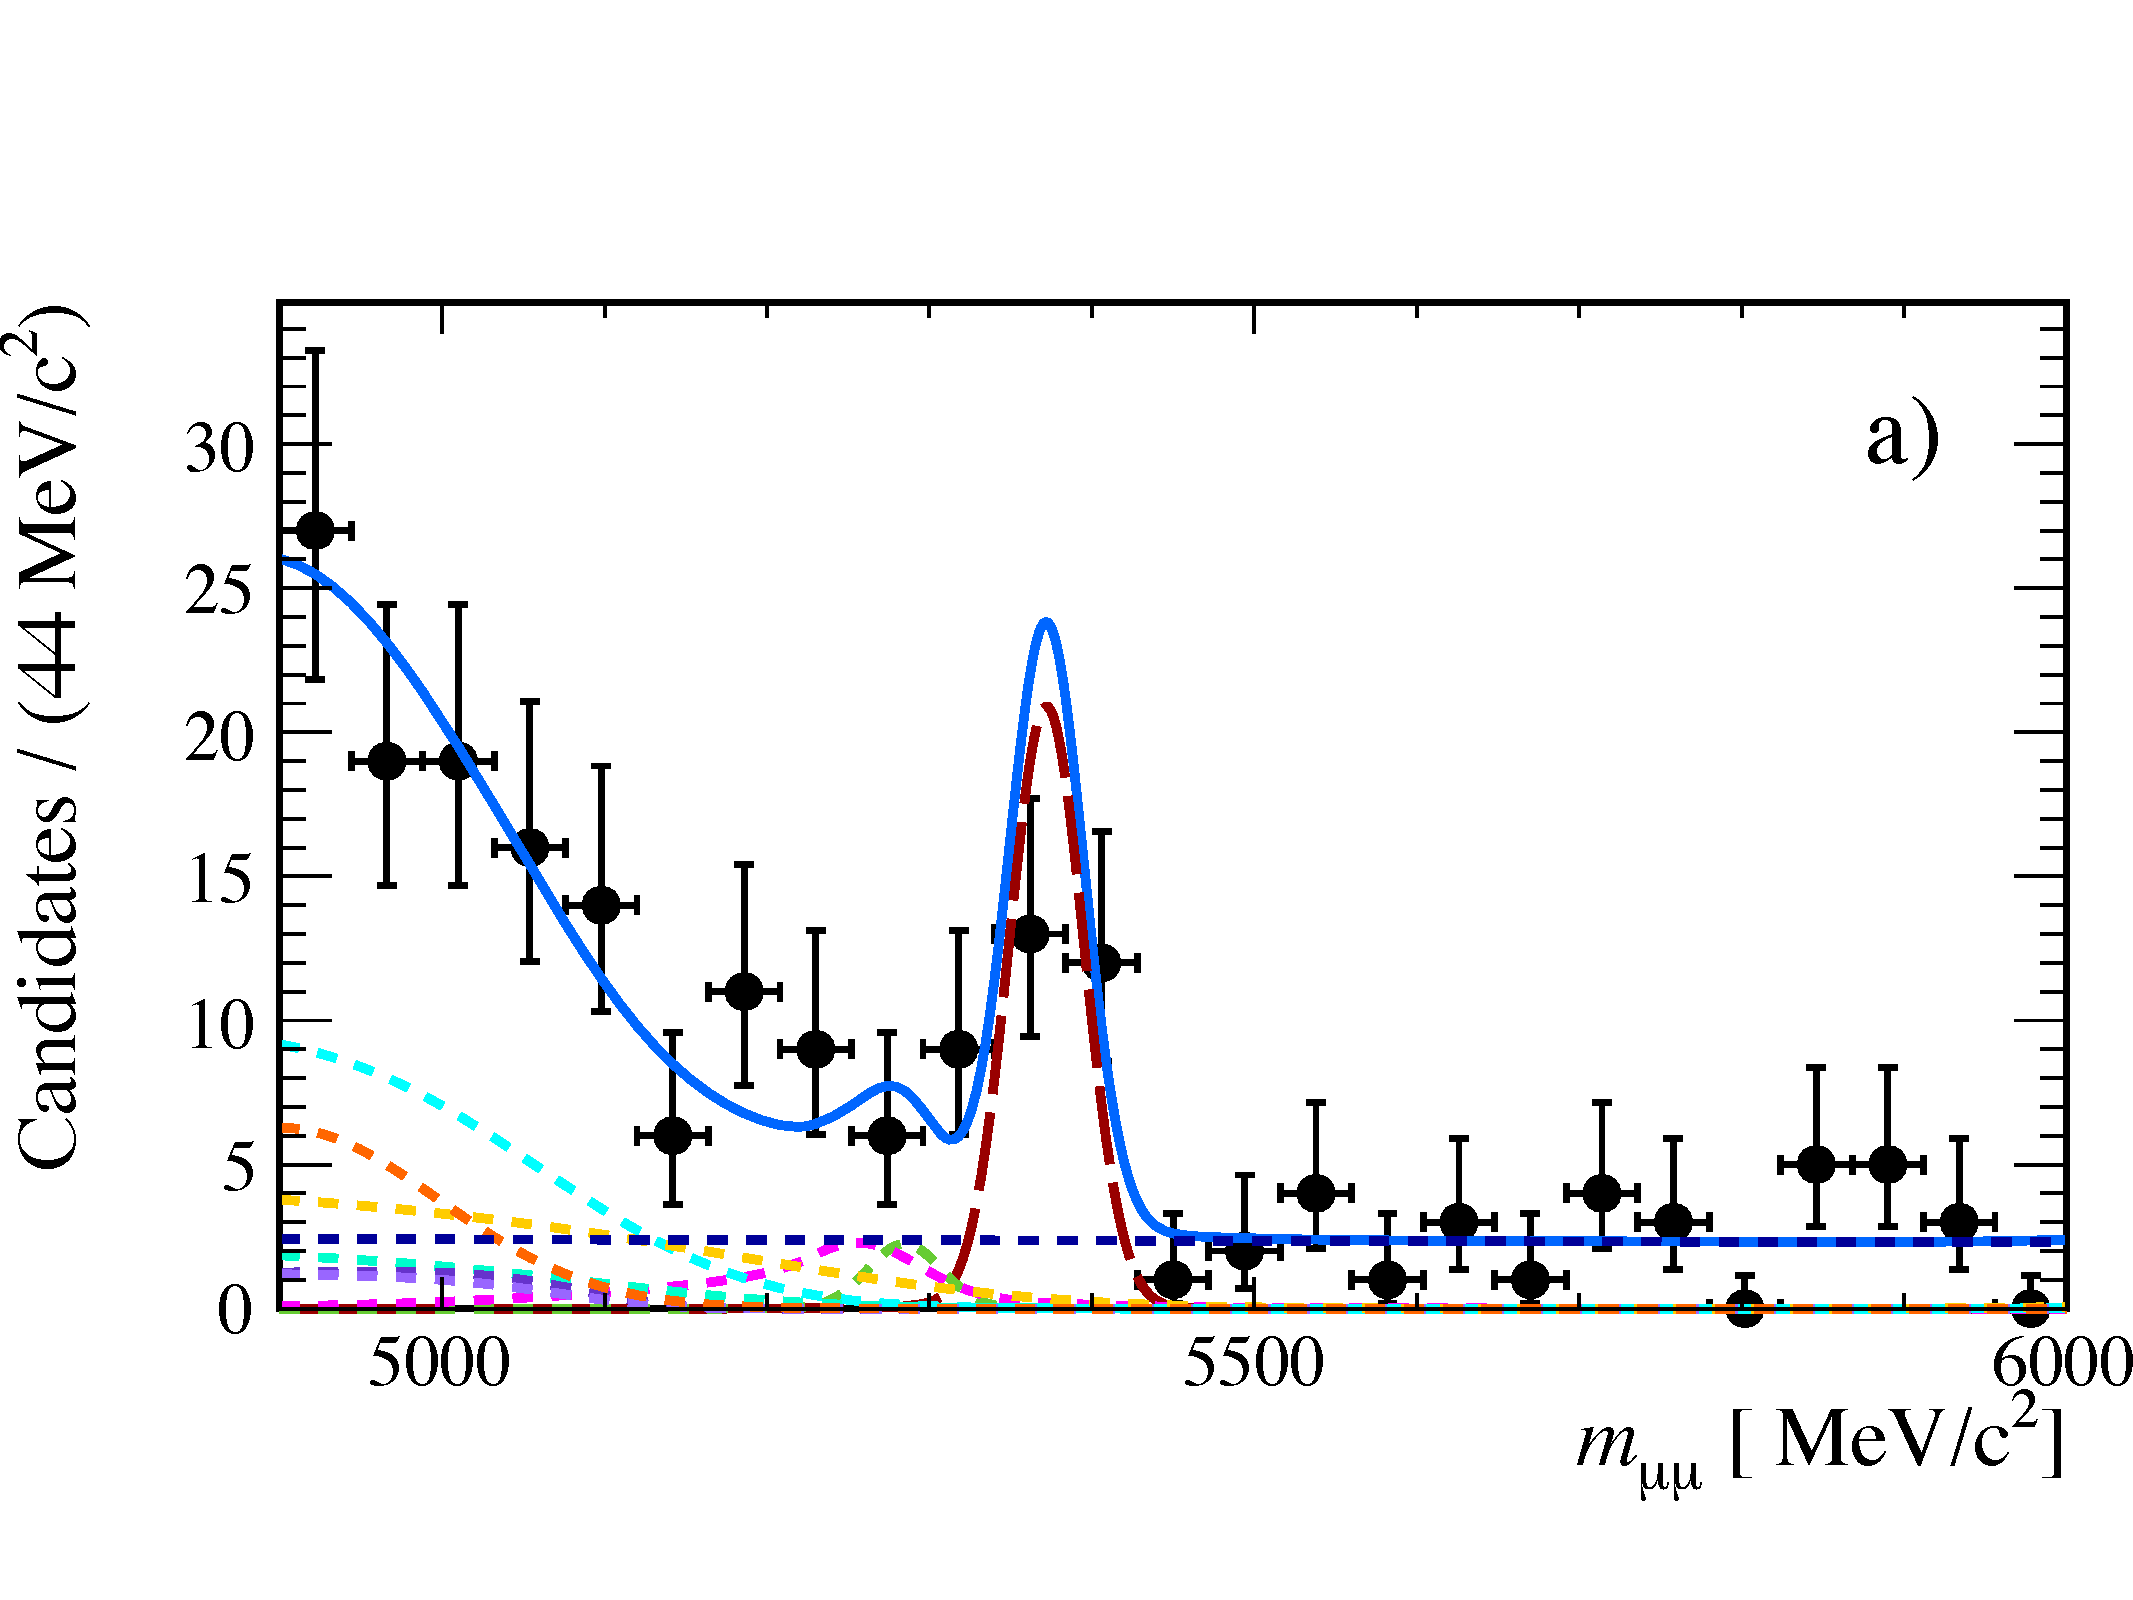
\includegraphics[width= 0.8 \textwidth]{./Figs/LifetimeMeasurement/mass_pdf2.pdf}
        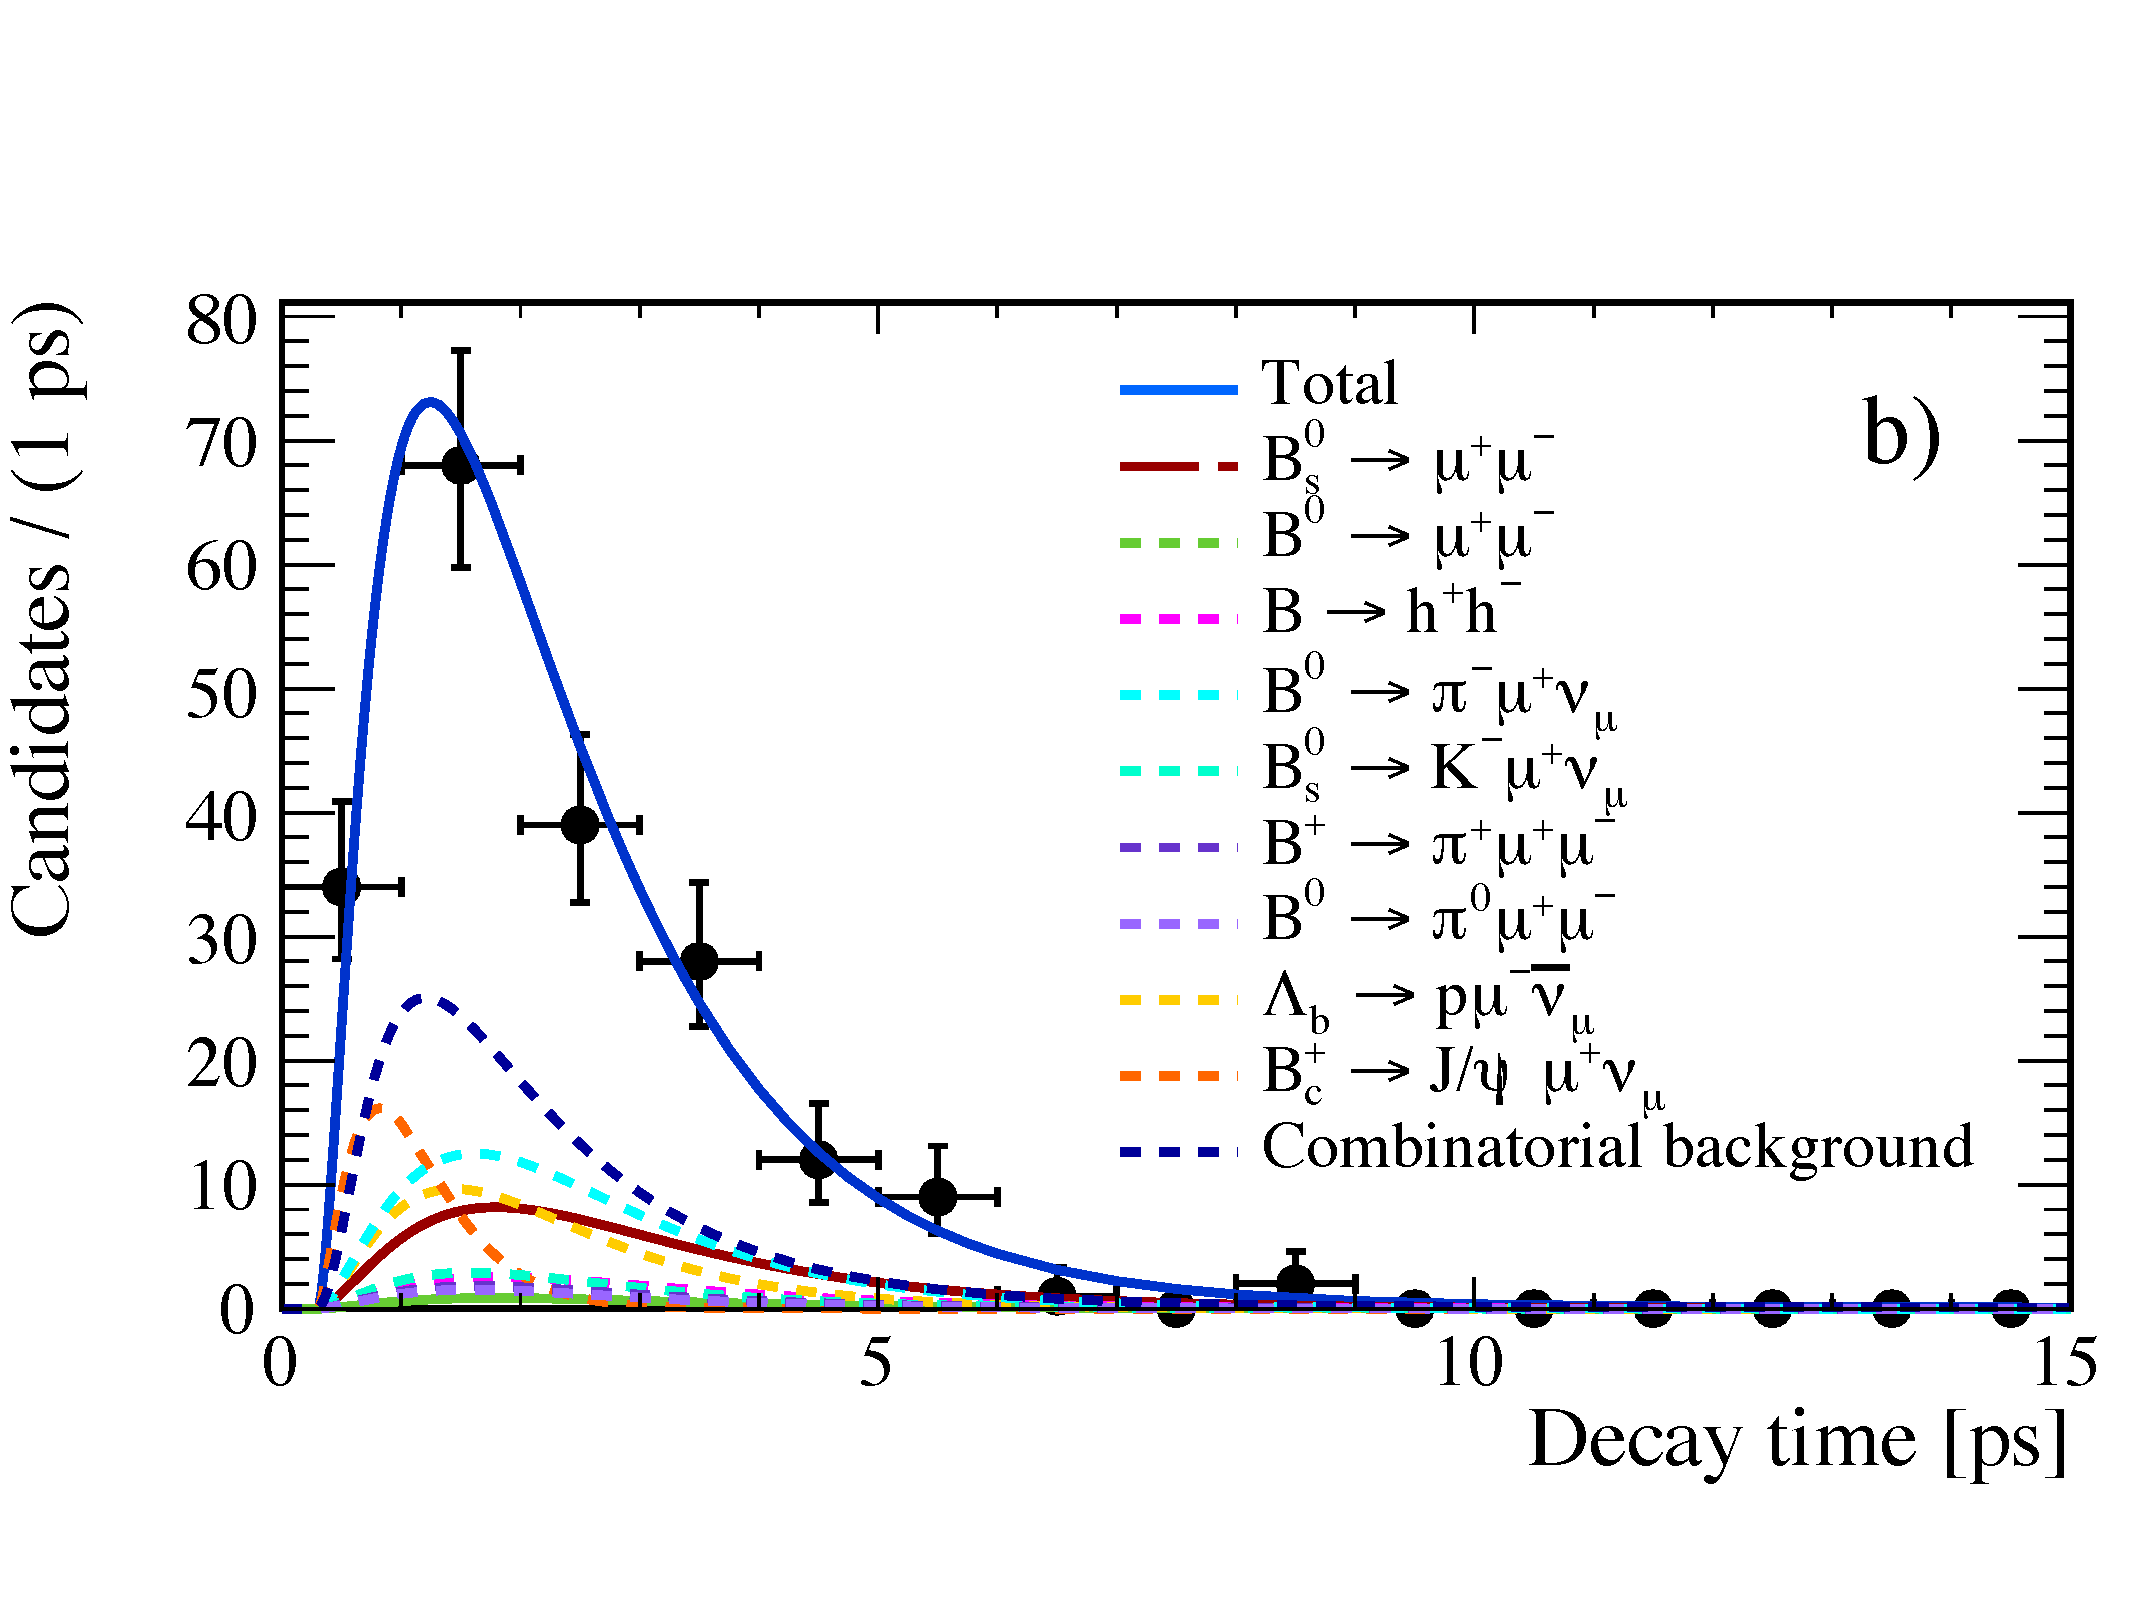
\includegraphics[width= 0.8 \textwidth]{./Figs/LifetimeMeasurement/DT_pdf2.pdf}
 
    \caption{Mass and decay time distributions for the generated decays in the mass range 4900 - 6000 for on pseudoexperiment.}
    \label{fig:toygen}
\end{figure}

\begin{table}[tb]
\begin{center}
\begin{tabular}{lclcc}
\toprule \toprule
Fit no.               & Mass Range  			 &  Components included in the mass \pdf & Yields & Yields \\ 
	               & /\mevcc 			  &				           & free  & fixed		\\ \midrule
\multirow{4}{*}{1.}	& \multirow{4}{*}{4900 - 6000}  &  \bsmumu, \bdmumu, comb. bkg.	& \checked & \\ \cmidrule{3-5}
                        &               		&  \bhh, \lambdab, \bcjpsimunu, 	& & \multirow{3}{*}{\checked} \\
			&				& \bdpimunu, \bsKmunu,  & &  \\ 
			&				&	\bupimumu, \bdpimumu   & &  \\ \midrule

\multirow{3}{*}{2.}	& \multirow{3}{*}{4900 - 6000} & \bsmumu, \bdmumu, comb. bkg.	& \checked & \\ \cmidrule{3-5}
                       &  				& \bhh, \lambdab, \bcjpsimunu, & & \multirow{2}{*}{\checked} \\
			&	&$B^{0}_{(s)} \to \pi^{-}(K^{-}) \mu^{+} \nu_{\mu}$, $B^{0(+)} \to \pi^{0(+)} \mu^{+}\mu^{-}$ & & \\  \midrule

\multirow{4}{*}{3.}	 & \multirow{4}{*}{5150 - 6000}  &  \bsmumu, \bdmumu, comb. bkg.	& \checked & \\ \cmidrule{3-5}
                        &               		  &  \bhh, \lambdab, \bcjpsimunu, & & \multirow{3}{*}{\checked} \\
			&				&	\bdpimunu, \bsKmunu,  & &  \\ 
			&				&	\bupimumu, \bdpimumu,  & &  \\ \midrule

\multirow{3}{*}{4.}	& \multirow{3}{*}{5150 - 6000} & \bsmumu, \bdmumu, comb. bkg.	& \checked & \\ \cmidrule{3-5}
                       &  				& \bhh, \lambdab, \bcjpsimunu & & \multirow{2}{*}{\checked} \\
				& & $B^{0}_{(s)} \to \pi^{-}(K^{-}) \mu^{+} \nu_{\mu}$, $B^{0(+)} \to \pi^{0(+)} \mu^{+}\mu^{-}$ & & \\  \midrule


\multirow{2}{*}{5.}	& \multirow{2}{*}{5200 - 6000} & \bsmumu, \bdmumu, comb. bkg.			&  \checked & \\ \cmidrule{3-5}
			&				  & \bhh, \lambdab, \bcjpsimunu			& 	& \checked  \\ \midrule
\multirow{2}{*}{6.}	& \multirow{2}{*}{5200 - 6000} & \bsmumu, \bdmumu, comb. bkg.			& \checked & \\ \cmidrule{3-5}
			&				&  \bhh, \lambdab 					& & \checked  \\ \midrule


7.			& 5200 - 6000 			& \bsmumu, \bdmumu, comb. bkg.			&  \checked &   \\ \midrule
8.			& 5200 - 6000 			& \bsmumu, comb. bkg.				& \checked &   \\ \midrule
9.			& 5250 - 6000 			& \bsmumu ,comb. bkg.				&    \checked & \\ \midrule
10.			& 5300 - 6000 			& \bsmumu, comb. bkg.				&  \checked &  \\ \midrule
11.			& 5320 - 6000 			& \bsmumu, comb. bkg.				&  \checked &  \\ \midrule
12.			& 5340 - 6000 			& \bsmumu, comb. bkg.				&  \checked &  \\ \midrule
13.			& 5350 - 6000 			& \bsmumu, comb. bkg.				&  \checked &  \\ \bottomrule \bottomrule
  
\end{tabular}
\vspace{0.7cm}
\caption{Mass ranges and components included in the different mass fit configurations tested using pseudoexperiments. The final two columns indicate which components in the mass fits have fixed yields at the expected value and which are left free in the fit. In fit configurations 2. and 4. a single mass \pdf is used to describe both \bdpimunu and \bsKmunu and a single \pdf is used to describe \bupimumu and \bdpimumu decays, all other configurations have one mass \pdf per component. The shapes for all mass \pdfs are fixed in the mass fit except the slope of the combinatorial background mass \pdf.}                                                                                                  
\label{tab:toyconfig}
\end{center}
\end{table}



\afterpage{
\begin{landscape}
\vspace*{\fill}
\begin{table}[hp]
\begin{center}
%\begin{tabular}{p{0.5cm}p{1.0cm}p{1.0cm}p{0.9cm}p{0.9cm}p{0.9cm}p{0.9cm}p{0.9cm}p{0.9cm}p{0.9cm}p{1.4cm}}
\begin{tabular}{lrrrrrrrrrr}
\toprule \toprule
Fit & \multicolumn{2}{c}{$\mathcal{N}$(\bsmumu)} & \multicolumn{2}{c}{$\mathcal{N}$(Comb. bkg.)} & \multicolumn{2}{c}{Comb. bkg. slope} & \tmumu & \multicolumn{3}{c}{\Gmumu} \\ \midrule
 &Mean&Width&Mean&Width&Mean&Width&$\sigma$/\ps&Mean&Width&$\sigma$/\ps$^{-1}$\\ \midrule
1. & -0.043 & 1.002 & -0.048 & 1.050 & -0.071 & 1.005 & 0.40 & 0.021 & 0.946 & 0.15 \\
2. & -0.064 & 1.015 & -0.018 & 1.048 & -0.092 & 1.006 & 0.35 & 0.013 & 0.970 & 0.13 \\
3. & -0.034 & 0.973 & -0.067 & 1.023 & -0.019 & 0.999 & 0.42 & 0.031 & 0.935 & 0.12 \\
4. & -0.042 & 0.981 & -0.066 & 1.024 & -0.018 & 0.999 & 0.41 & 0.028 & 0.942 & 0.15 \\
5. & -0.094 & 0.997 & 0.100 & 1.007 & -0.228 & 1.018 & 0.40 & 0.017 & 0.933 & 0.40 \\
6. & -0.124 & 1.024 & 0.110 & 1.009 & -0.242 & 1.021 & 0.32 & -0.008 & 0.973 & 0.12 \\
7. & -0.367 & 1.045 & 1.248 & 0.923 & -1.823 & 1.104 & 0.33 & -0.091 & 0.975 & 0.12 \\
8. & -0.521 & 1.049 & 1.770 & 0.983 & -2.425 & 1.075 & 0.34 & -0.114 & 0.969 & 0.12 \\
9. & -0.473 & 1.044 & 1.296 & 0.918 & -1.883 & 1.126 & 0.34 & -0.126 & -.993 & 0.12 \\
10. & -0.101 & 1.013 & 0.396 & 0.989 & -0.571 & 1.068 & 0.31 & -0.043 & 0.985 & 0.11 \\
11. & 0.050 & 1.006 & 0.060 & 1.013 & -0.123 & 1.013 & 0.29 & 0.024 & 0.982 & 0.11  \\
12. & 0.020 & 1.009 & 0.015 & 1.007 & -0.066 & 0.991 & 0.30 & 0.021 & 0.995 & 0.11 \\
13. & 0.007 & 1.001 & -0.039 & 1.033 & -0.029 & 0.995 & 0.34 & 0.023 & 0.983 & 0.13 \\ \bottomrule \bottomrule
\end{tabular}
\vspace{0.7cm}
\caption{Results for the pseudoexperiments testing the mass fit configurations. The mean and width of the pull distributions for the \bsmumu and combinatorial background yields and the slope of the combinatorial background mass \pdf are shown along with the expected statistical uncertainty on \tmumu and \Gmumu. The uncertainties on the means are 0.010 and the widths are 0.007 for all configurations.}                                                                                                   
\label{tab:toyResults}
\end{center}
\vspace{-1.0cm}                                                                                                                                               
\end{table}
\vspace*{\fill}
\end{landscape}
}

%\vspace*{\fill}%These are the original number that I ran, but I couldn’t get the correct systematics with these toys. Also I think the lifetime range was too long at 0 - 15 ps. Finally the buffer was set of 0.5 which gives some errors
%\afterpage{
%\begin{landscape}
%\vspace*{\fill}
%\begin{table}[hp]
%\begin{center}
%\begin{tabular}{p{0.5cm}p{1.0cm}p{1.0cm}p{0.9cm}p{0.9cm}p{0.9cm}p{0.9cm}p{0.9cm}p{0.9cm}p{0.9cm}p{1.4cm}}
%\begin{tabular}{lcccccccccc}
%\bottomrule \bottomrule
%Fit & \multicolumn{2}{c}{$\mathcal{N}$(\bsmumu)} & \multicolumn{2}{c}{$\mathcal{N}$(Comb.)} & \multicolumn{2}{c}{$\lambda$} & \tmumu & \multicolumn{3}{c}{\Gmumu} %\\ \bottomrule \bottomrule
% &Mean&Width&Mean&Width&Mean&Width&$\sigma$/\ps&Mean&Width&$\sigma$/\ps$^{-1}$\\ \bottomrule \bottomrule
%1. & -0.04 & 1.00 & -0.05 & 1.05 & 0.06 & 1.00 & 0.38 & 0.03 & 0.95 & 0.14 \\
%2. & -0.06 & 1.01 & -0.05 & 1.05 & 0.09 & 1.01 & 0.37 & -0.01 & 0.96 & 0.13 \\
%3. & -0.04 & 0.99 & -0.08 & 1.03 & -0.04 & 0.99 & 0.41 & 0.00 & 0.94 & 0.15 \\
%4. & -0.03 & 0.99 & -0.10 & 1.02 & -0.03 & 1.00 & 0.40 & 0.03 & 0.96 & 0.15 \\
%5. & -0.11 & 0.99 & 0.10  & 1.03 & -0.25 & 1.04 & 0.40 & 0.00 & 0.95 & 0.15 \\
%6. & -0.15 & 1.03  & 0.09 & 1.02 & -0.17 & 1.02 & 0.31 & -0.01 & 0.98 & 0.11 \\
%7. &0.36 & 1.05  & 1.25& 0.93 & -1.62 & 1.11 & 0.32 & -0.12 & 0.99 & 0.11 \\
%8. &-0.52 & 1.05 & 1.73 & 0.89 & -2.23 & 1.08 & 0.33 & -0.15 & 0.99 & 0.12 \\
%9. & 0.45 & 1.04 & 1.29 & 0.91 & -1.78 & 1.13 & 0.33 & -0.14 & 0.99 & 0.12 \\
%10. & -0.08 & 1.03 & 0.36 & 0.98 & -0.49 & 1.06 & 0.30 & -0.05 & 1.00 & 0.11 \\
%11. &0.00 & 1.01 & 0.06 & 1.02 & -0.10 & 1.02 & 0.29 & 0.00 & 1.00 & 0.11 \\ \bottomrule \bottomrule
%This will not be the same as the systematic Fit Accuarcy part since all backgrounds are generated here!
%\end{tabular}
%\vspace{0.7cm}
%\caption{Results for the toy studies testing the mass fit configuration. The mean and width of the pull distributions for the \bsmumu and combinatorial %background yields and the slope of the combinatorial background mass \pdf, $\lambda$, are shown along with the expected statistical uncertainty on \tmumu and %\Gmumu. The uncertainties on the means and widths are 0.01 for all configurations.}                                                                                                   
%\label{tab:toyResults}
%\end{center}
%\vspace{-1.0cm}                                                                                                                                               
%\end{table}
%\end{landscape}
%}
%\vspace*{\fill}

%\pagebreak


Therefore, the fit configuration number 11 is chosen to measure the \bsmumu effective lifetime. Figure~\ref{fig:toyegs} gives an example of the mass and decay time \ml fits for the chosen configuration Figure~\ref{fig:toygen} shows that the number of background decays from \bdmumu, \bhh and \lambdab is extremely low above 5320 \mevcc therefore these backgrounds do not need to be modelled in the mass \pdf. The affect on the final result of not modelling these backgrounds is estimated in Section~\ref{sec:BKGcontaim}.

\begin{figure}[tbp]
    \centering
        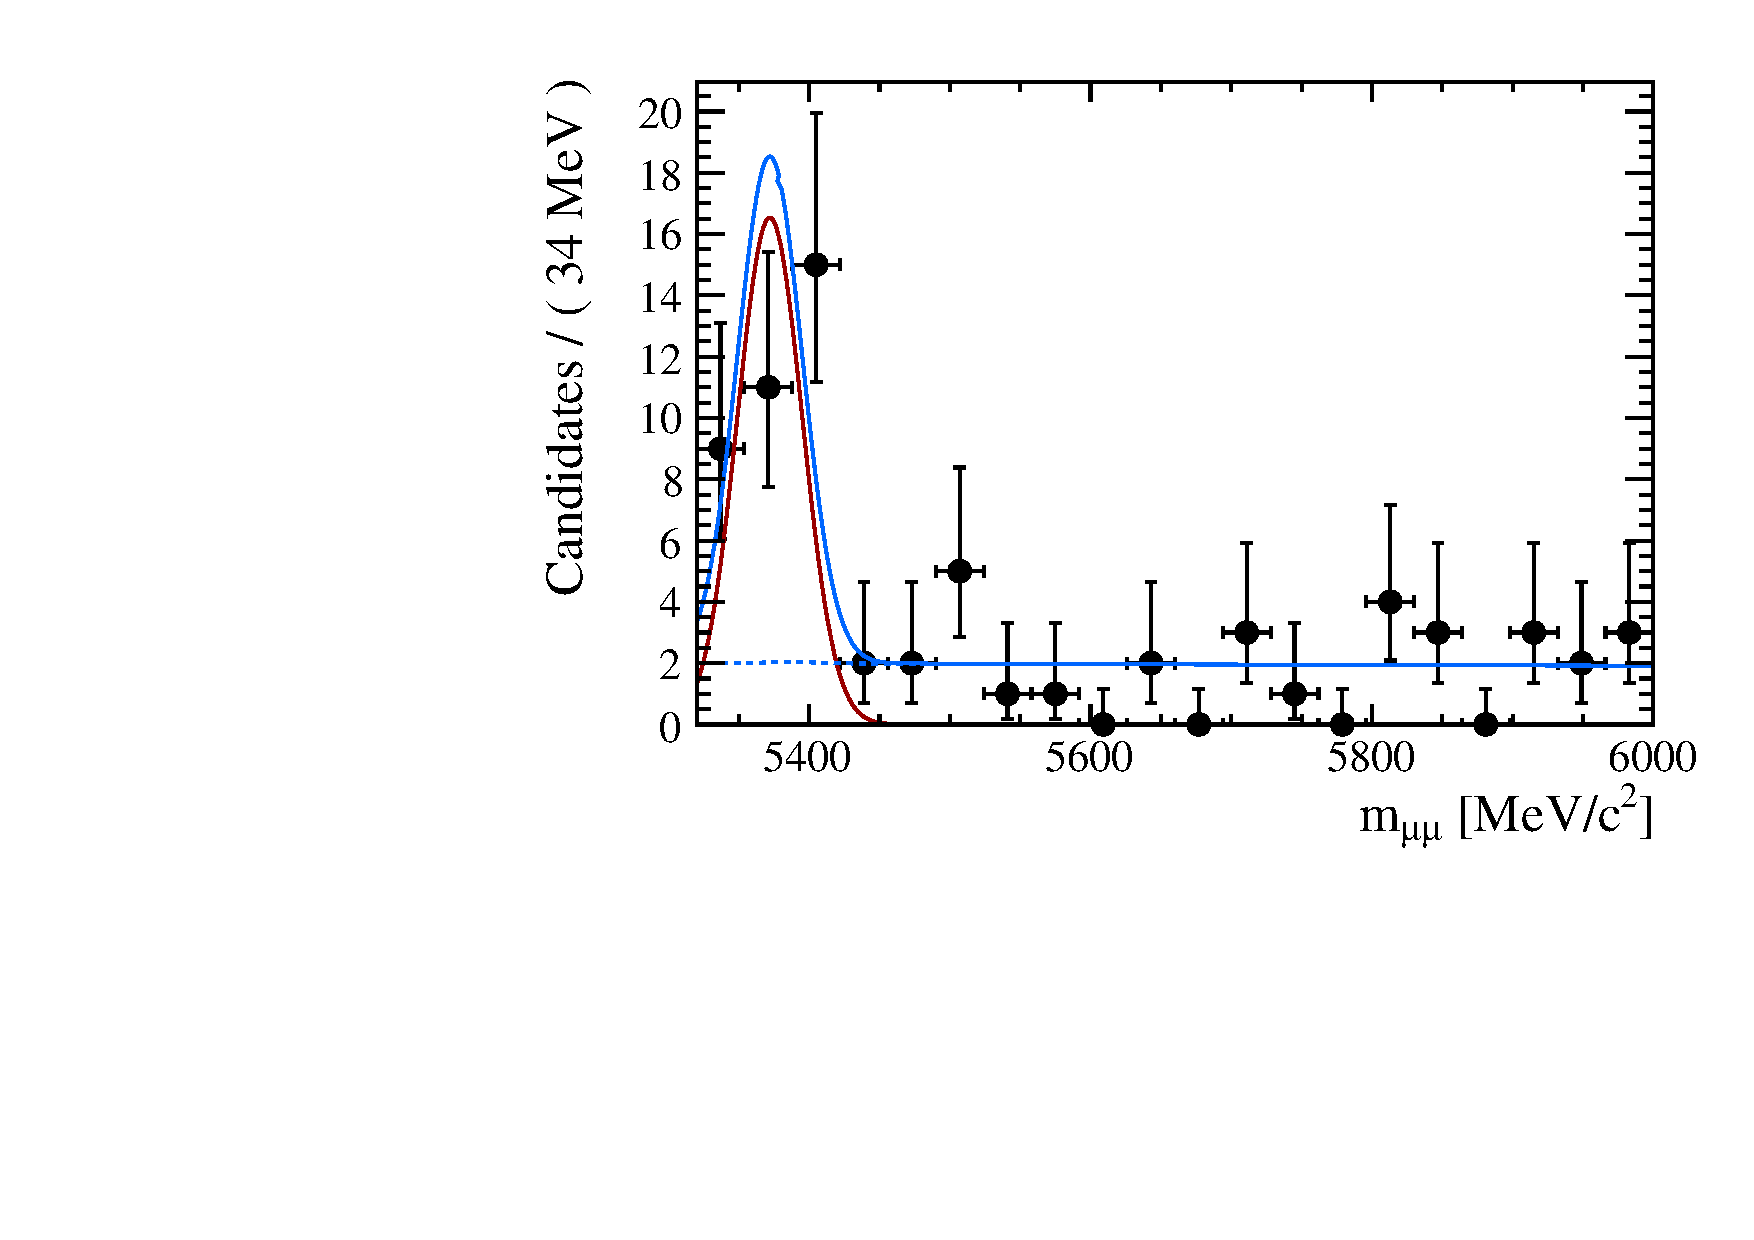
\includegraphics[width= 0.49 \textwidth]{./Figs/LifetimeMeasurement/5320-6000_toy_mass.pdf}
       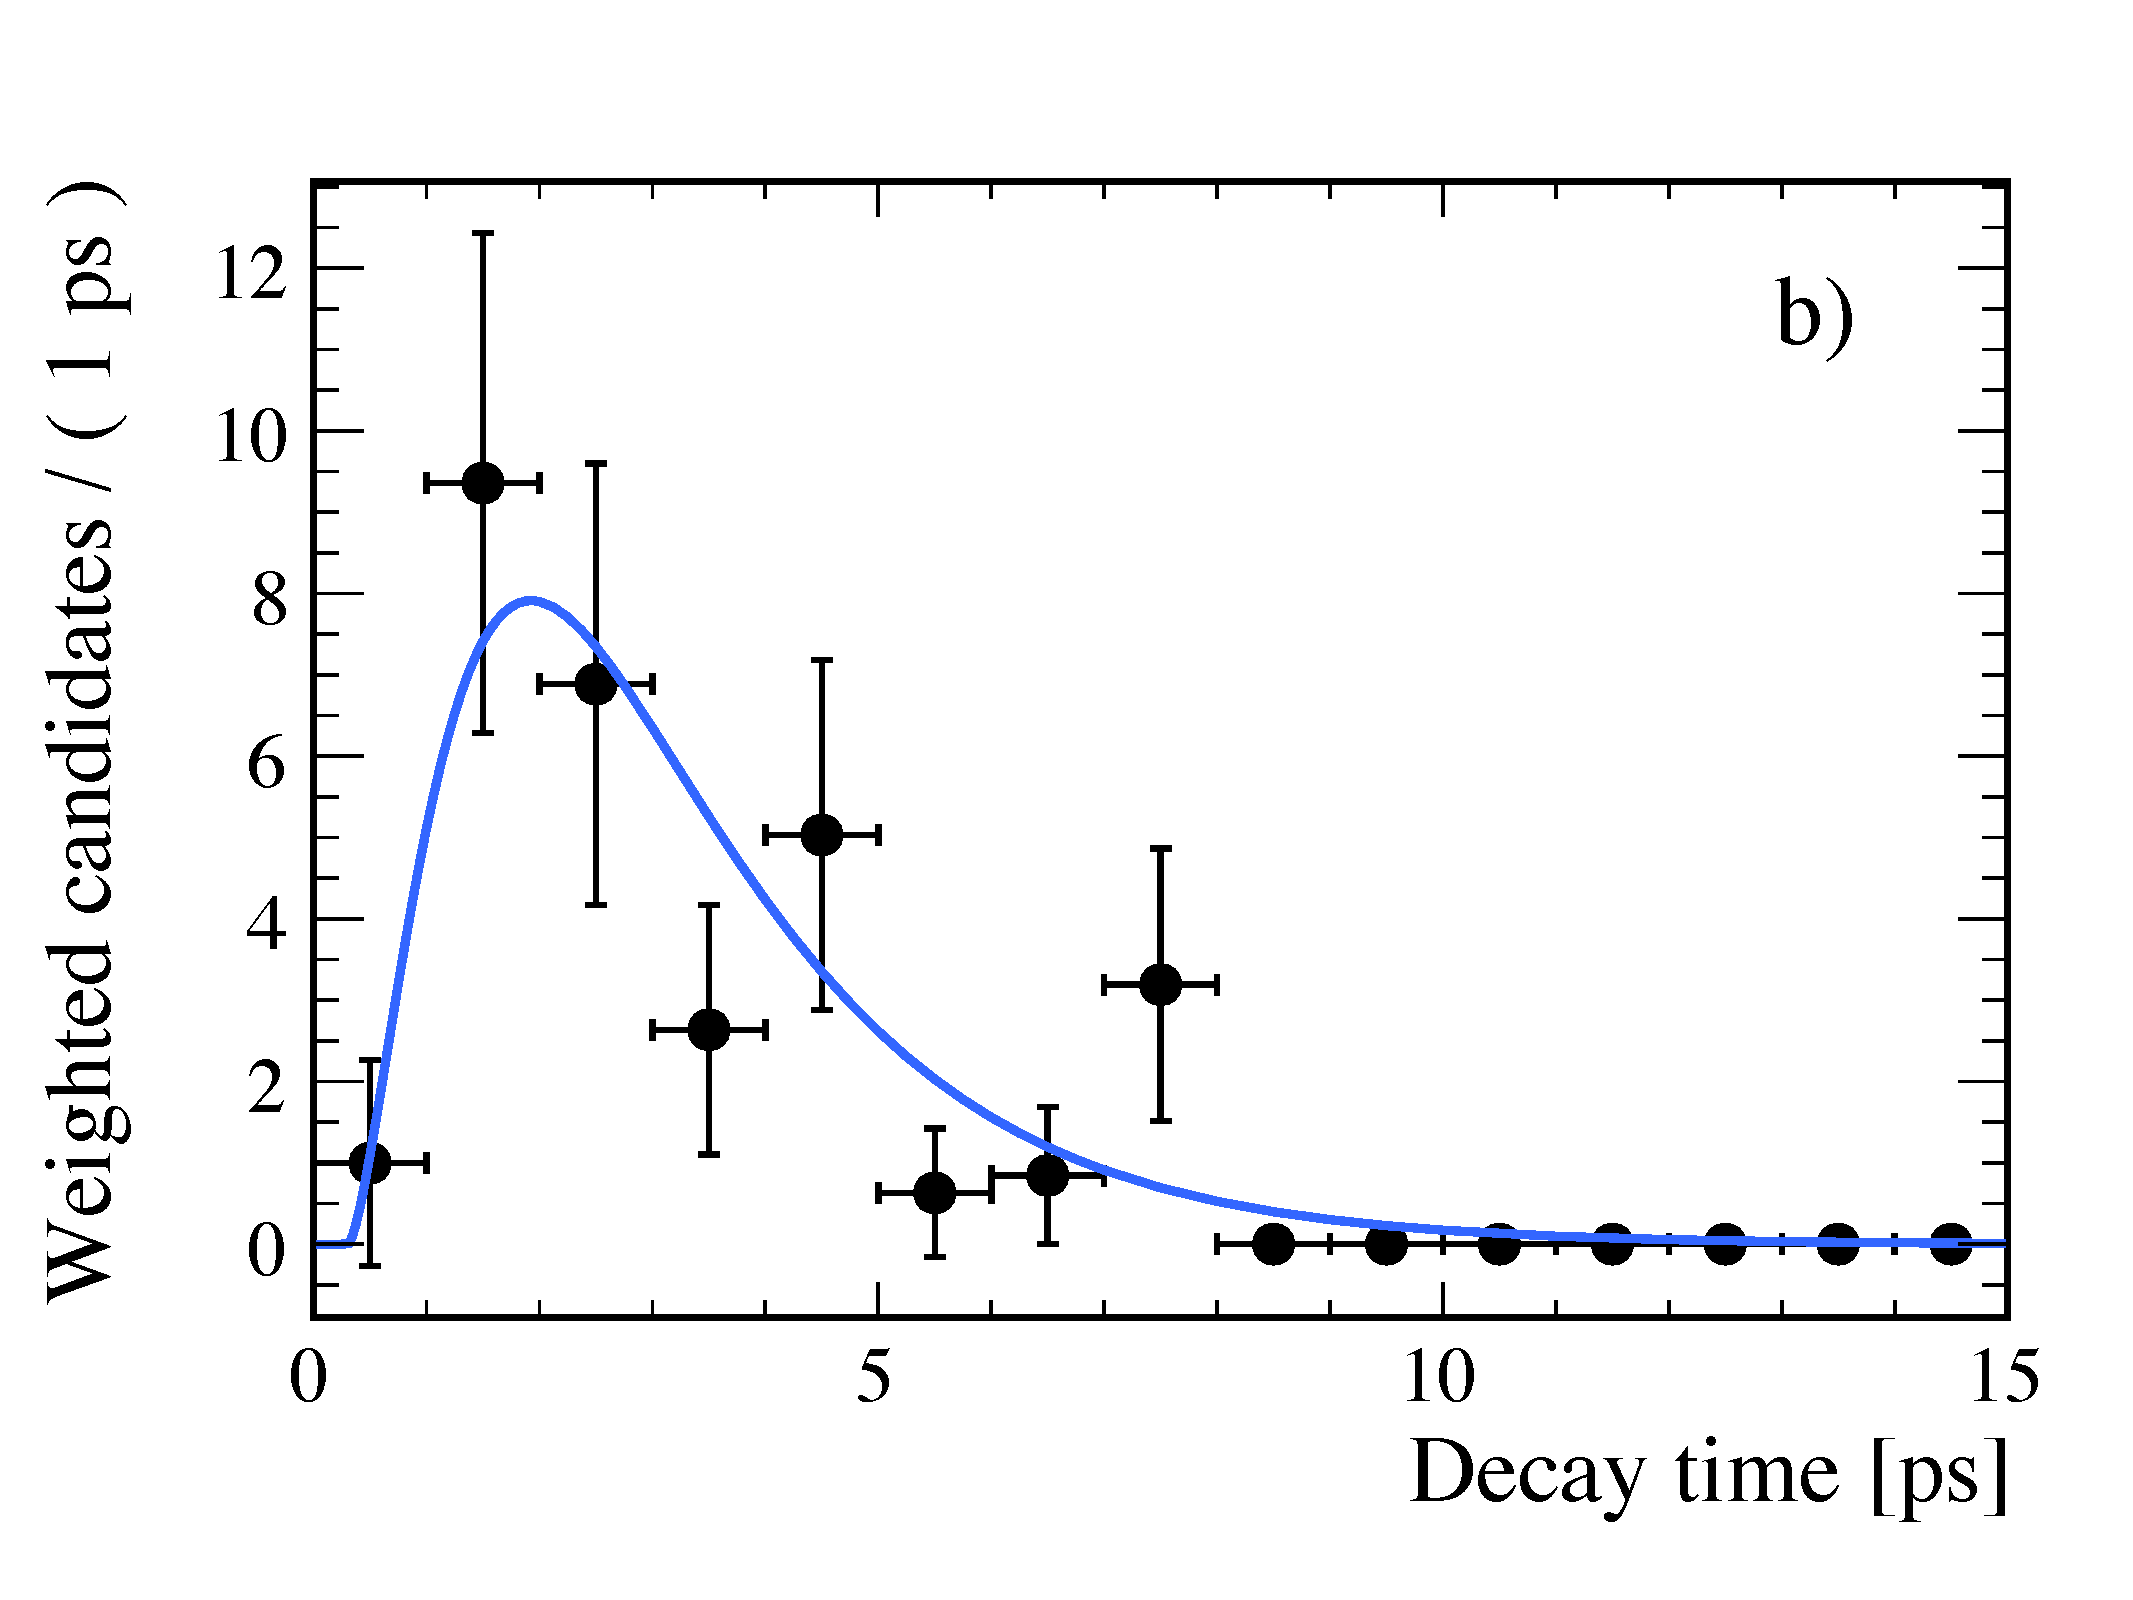
\includegraphics[width=0.49 \textwidth]{./Figs/LifetimeMeasurement/5320-6000_toy_lifetime.pdf}
    \caption{Example of the mass and decay time \ml fits for one pseudoexperiment using the chosen fit configuration where only components for \bsmumu and combinatorial background are modelled in the mass \pdf.}
    \label{fig:toyegs}
\end{figure}

The expected uncertainties for the chosen fit configuration for \tmumu and \Gmumu are $\sigma \left ( \tau_{\mu\mu}  \right ) = $ 0.28 ps and  $\sigma \left ( \Gamma_{\mu\mu}  \right ) = $ 0.11 \ps$^{-1}$. However, due to the low expected number of decays there is a large spread in the expected uncertainties as shown in Figure~\ref{fig:exptuncert}. Therefore the uncertainties on the measurements would range between 0.1 - 0.8 ps for \tmumu and 0.07 - 0.2 \ps$^{-1}$ for \Gmumu.


\begin{figure}[tbp]
    \centering
        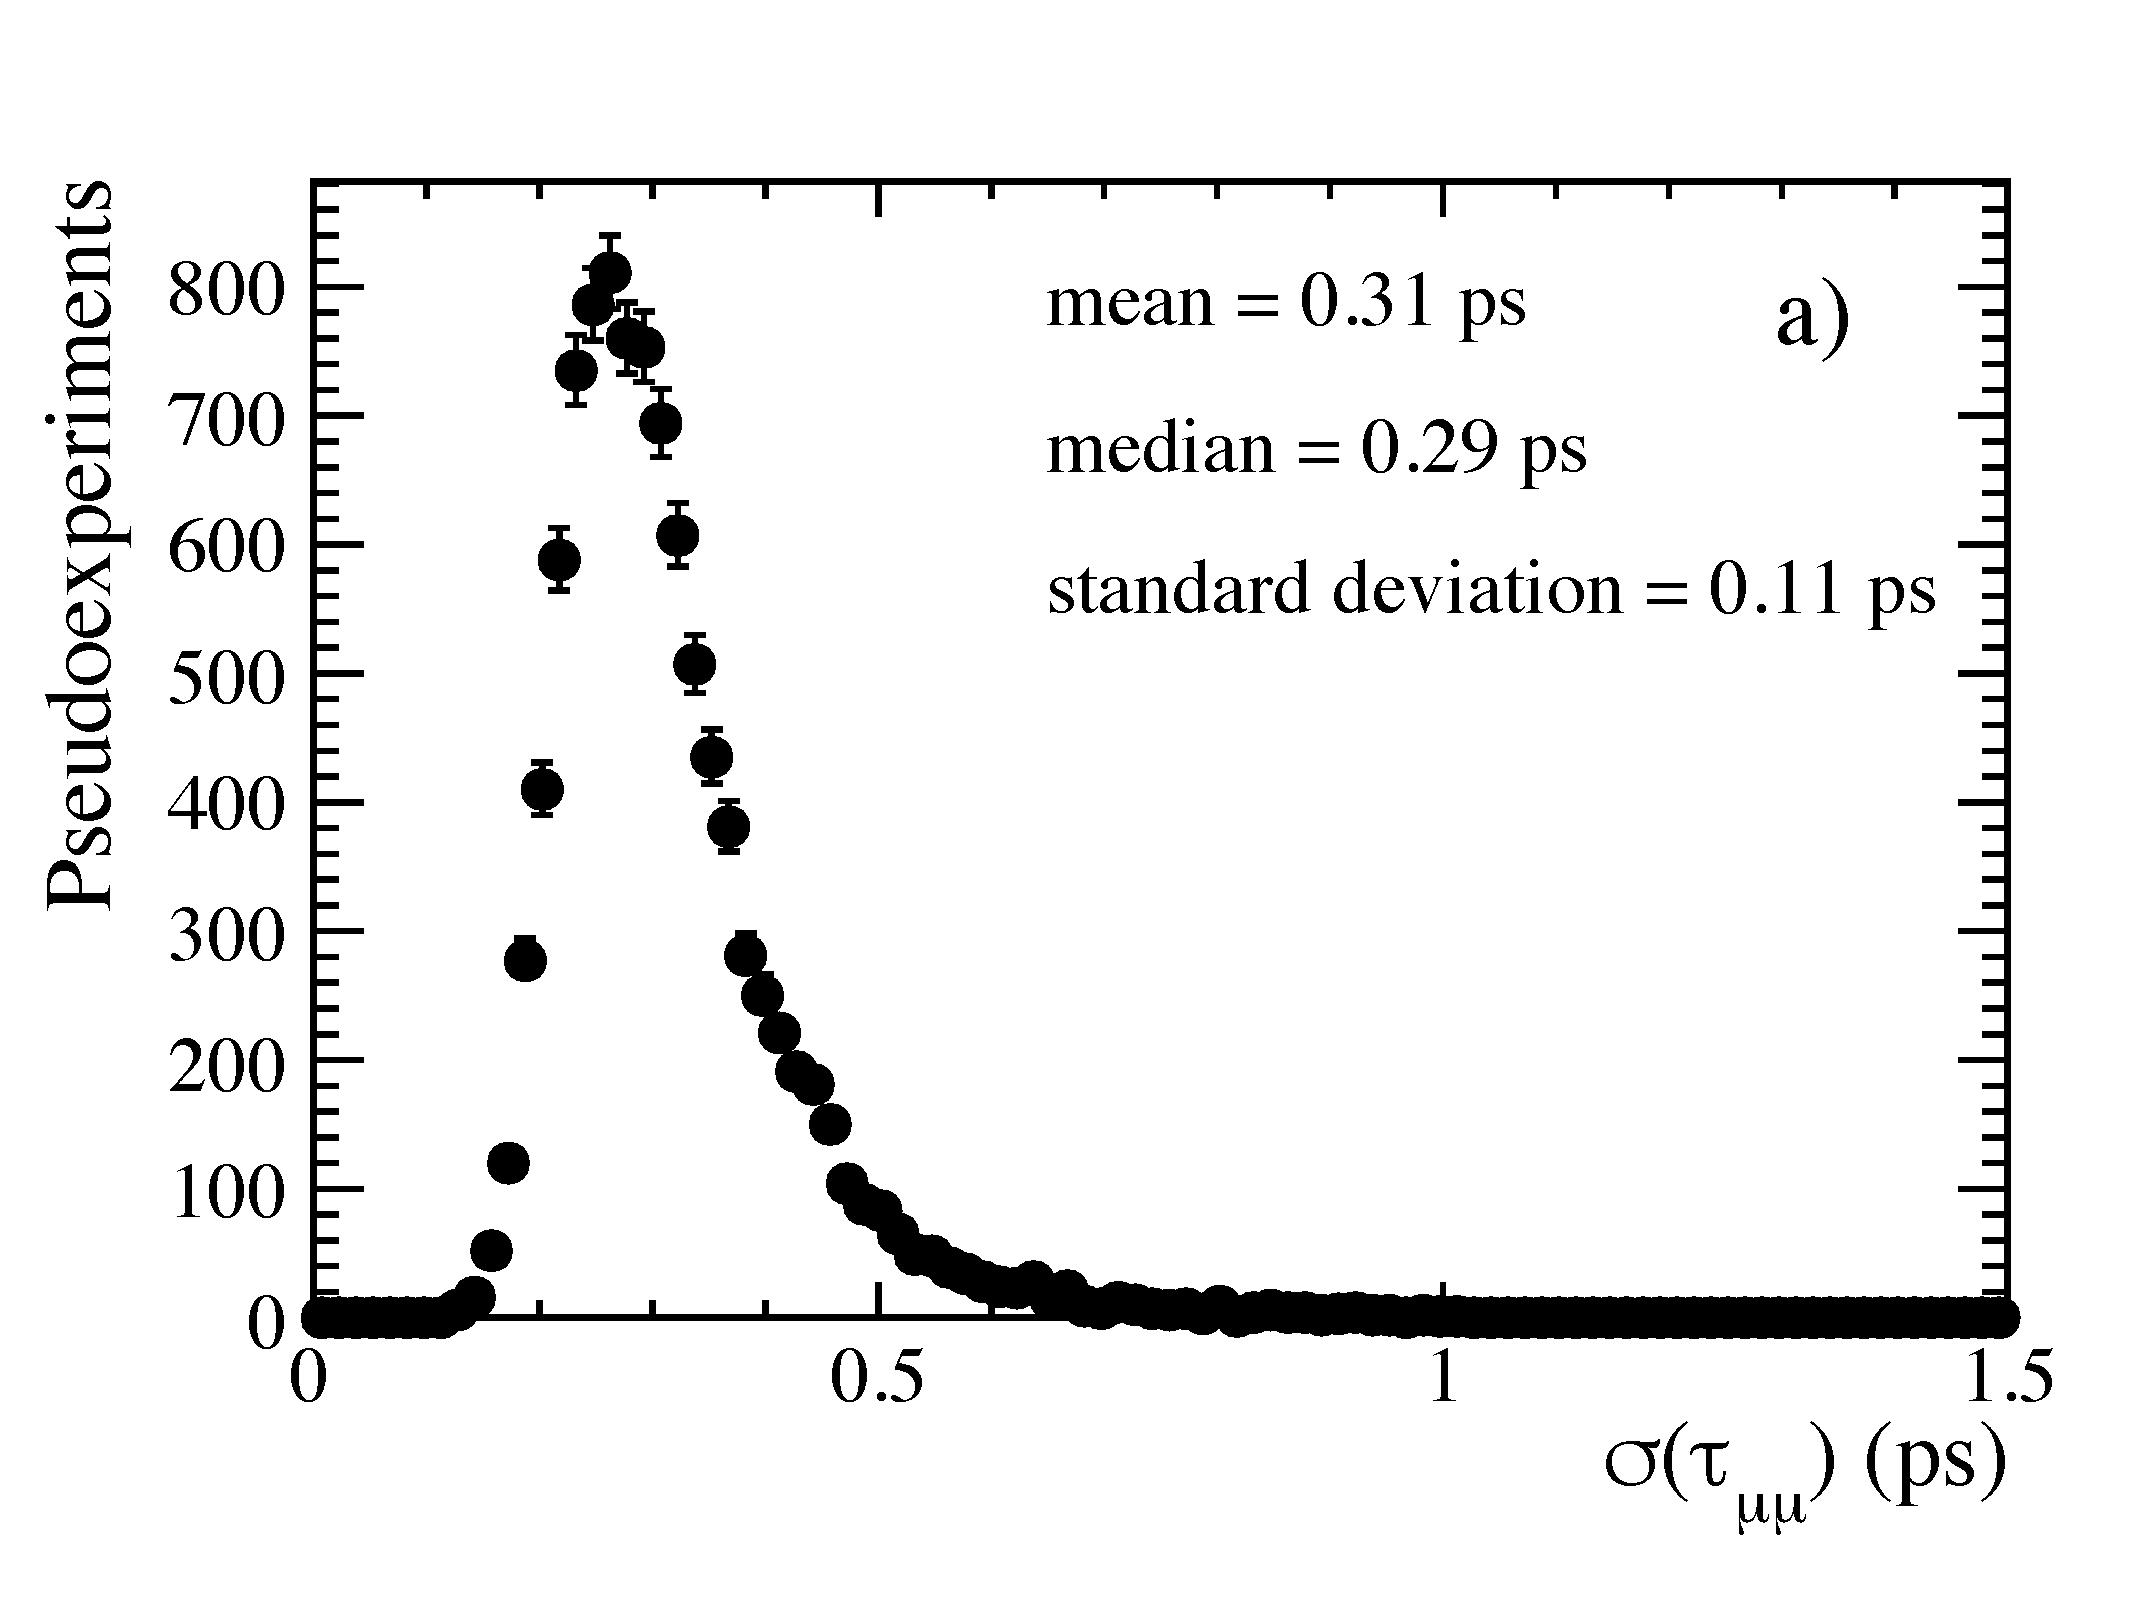
\includegraphics[width=0.49 \textwidth]{./Figs/LifetimeMeasurement/5320-6000_tau_err.pdf}
        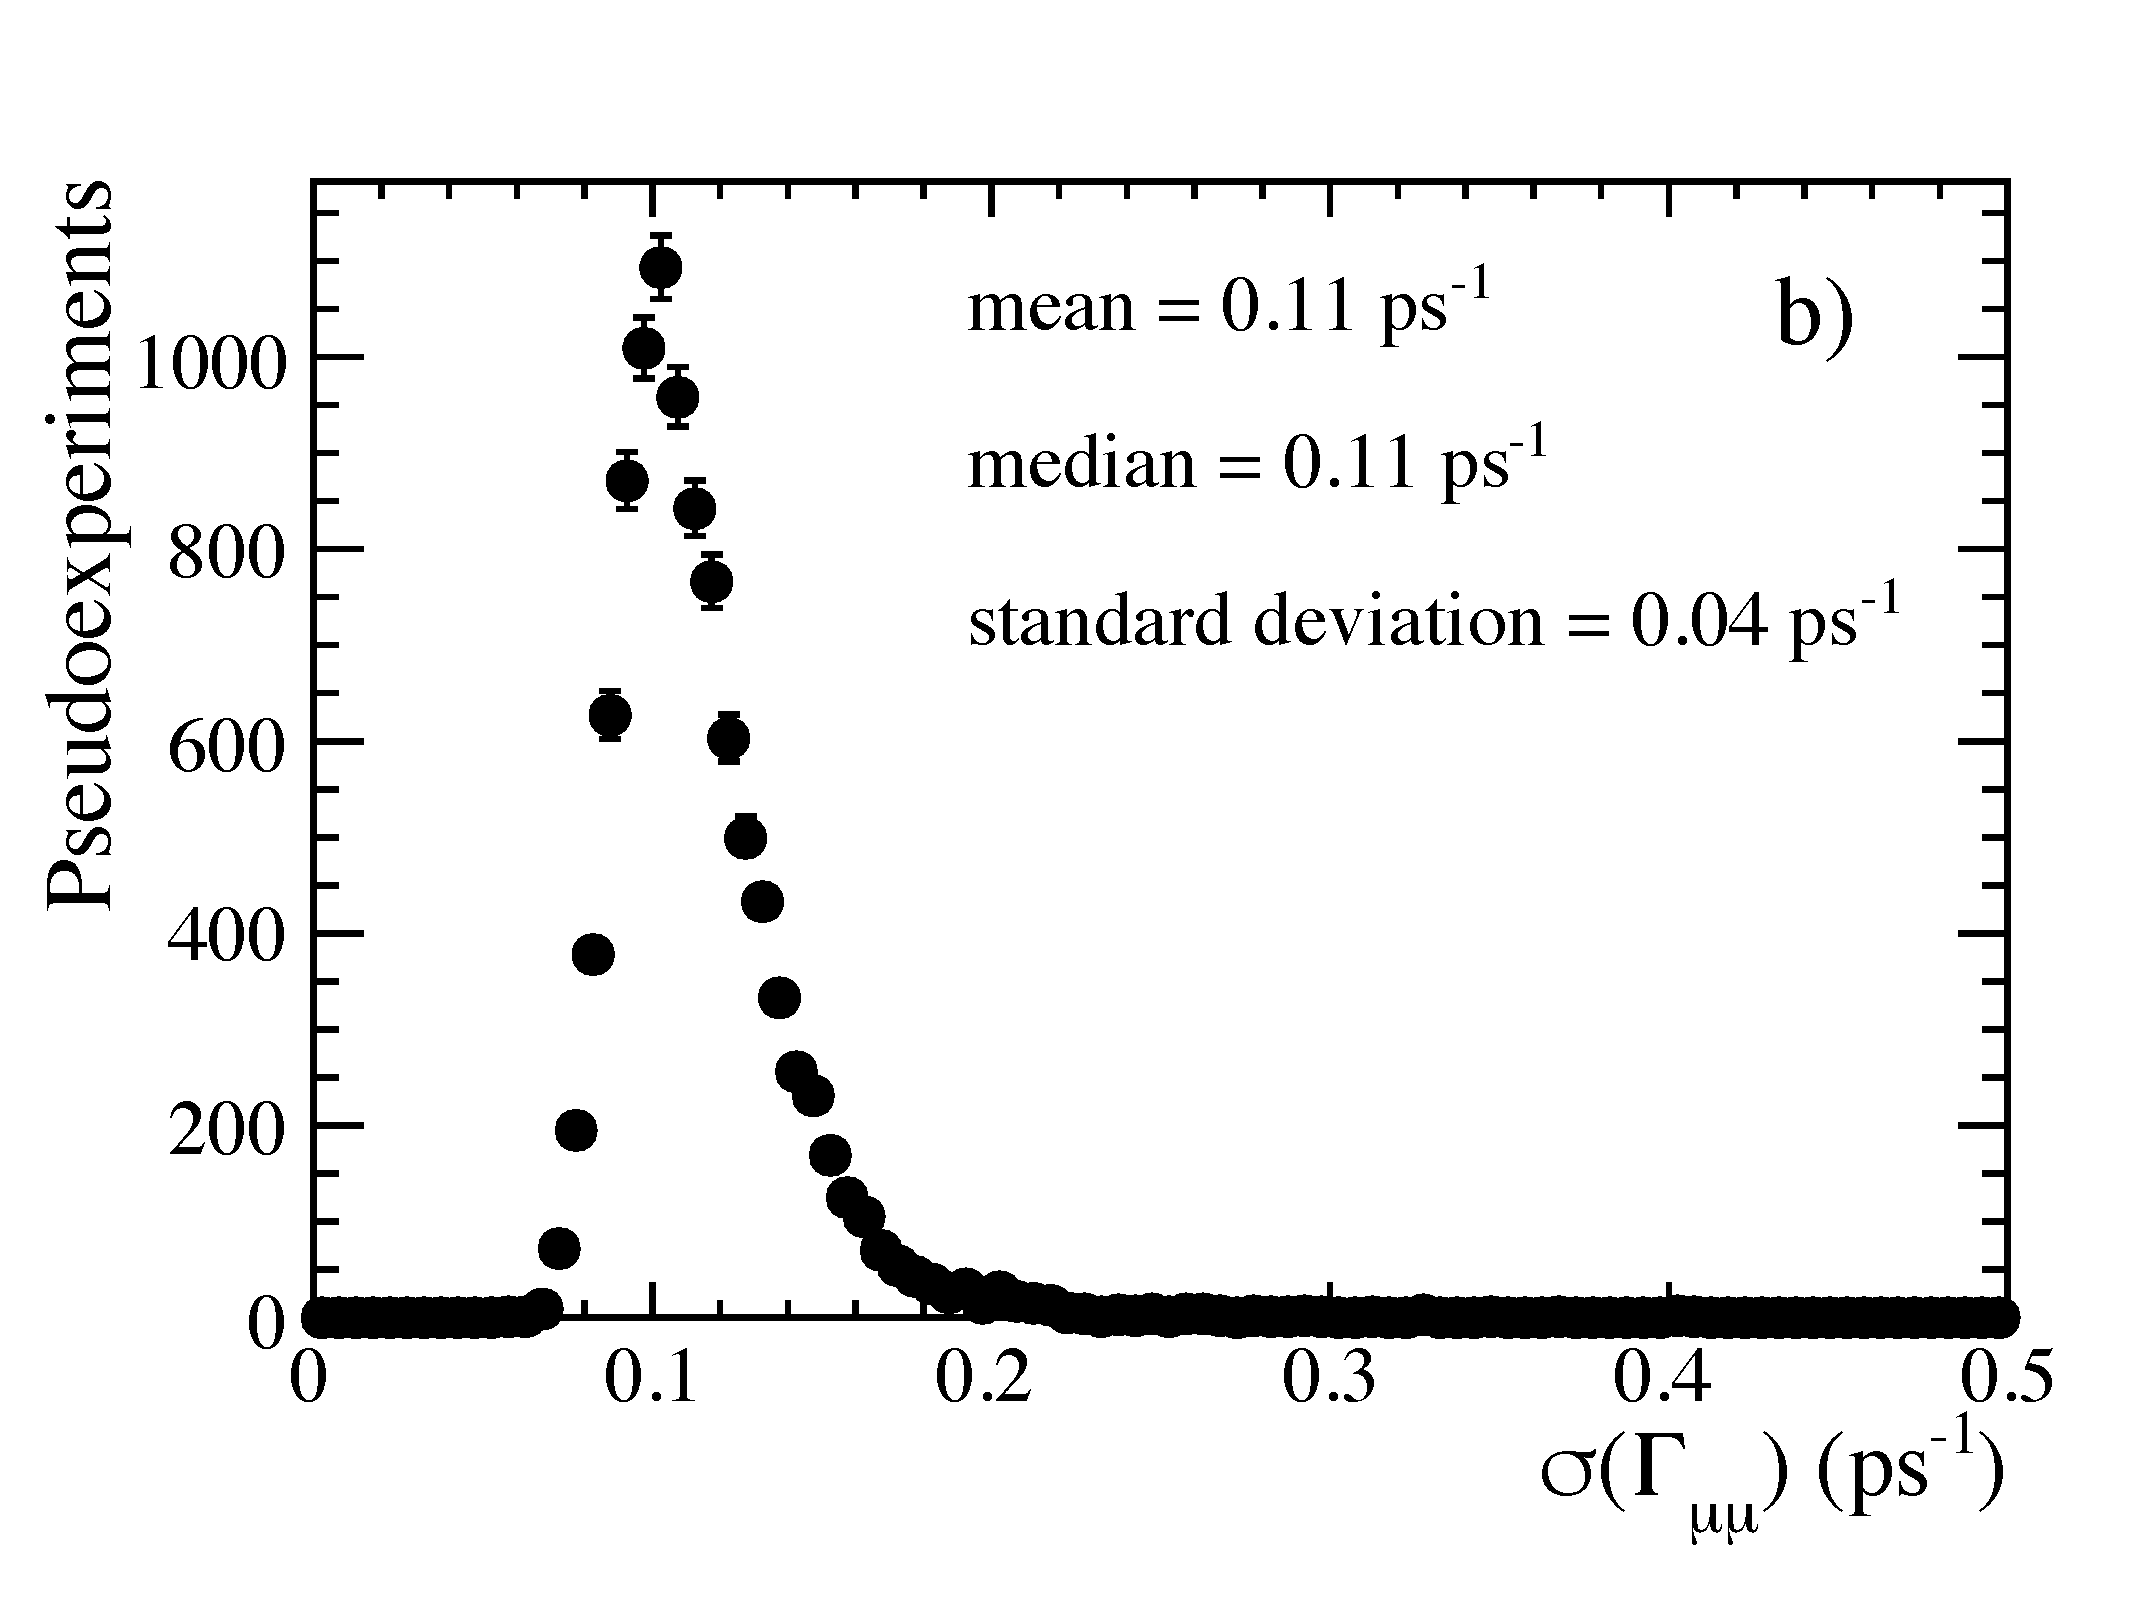
\includegraphics[width=0.49\textwidth]{./Figs/LifetimeMeasurement/5320-6000_gamma_err.pdf}

    \caption{Expected statistical uncertainties for \tmumu (left) and \Gmumu (right) using fit configuration number 11.}
    \label{fig:exptuncert}
\end{figure}


\section{Results}
\label{sec:ELresults}

The results of the unbinned \ml fit to the dimuon mass distribution and the sWeighted decay time of \bsmumu candidates for 4.4~\fb of Run 1 and Run 2 data are shown in Figure~\ref{fig:ELresults}. The number of observed decays was 22 $\pm$ 6 \bsmumu decays and 20 $\pm$ 6 combinatorial background decays. The measured values of \tmumu and \Gmumu are
\begin{equation}
\tau_{\mu\mu} = 2.04 \pm 0.44  \text{ ps} 
\end{equation}
\begin{equation}
\Gamma_{\mu\mu} = 0.489  \pm 0.117 \text{ ps}^{-1}
\end{equation}
where the uncertainties are only statistical. The results are consistent with the Standard Model prediction of \tmumu = \tH within  1 $\sigma$ and within  1.5 $\sigma$ of \tmumu = \tL.

The observed number of signal and background decays is lower than expected yields given in Table~\ref{tab:expectedevents}.
Therefore, it is important to check whether the statistical coverage for \tmumu uncertainties is still reasonable. The pseudoexperiments in Section~\ref{sec:tauORinvtau} were repeated, this time using the observed number of \bsmumu and combinatorial background decays and the results are shown in Table~\ref{tab:LifetimeCoverage_observed}. The statistical coverage of the \tmumu uncertanity is good and therefore \tmumu and its statistical uncertainty can be trusted as accurate.

%the statistical coverage of the \tmumu and \Gmumu uncertainties is re-calculated using pseudoexperiments generated with the observed number of decays. In the pseudoexperiments all the background decays are generated at the expected level. The coverage of both \tmumu and \Gmumu statistical uncertainties is good, as shown in Table~\ref{tab:LifetimeCoverage_observed}, therefore the result of the more interesting \tmumu and its statistical uncertainty can be trusted as accurate. %The bias introduced by the fit strategy is estimated in Chapter X. 

\begin{table}[hb]
\begin{center}
\begin{tabular}{lccc}
\toprule \toprule
 & \tmumu &  \Gmumu & Gaussian \\ \midrule 
$1\sigma$ & 68.83 $\pm$0.08\% & 67.76$\pm$0.08\% & 68.27\% \\
$2\sigma$ &  93.11$\pm$0.10\% & 95.55$\pm$0.10\% &  95.45\% \\
$3\sigma$ & 97.92$\pm$0.10\% &  99.67$\pm$0.10\% & 99.73 \% \\ \bottomrule \bottomrule
\end{tabular}
\vspace{0.7cm}                                                                                                                                               
\caption{Coverage of the statistical uncertainties evaluated as the number of pseudoexperiments using the observed number of decays with measured \tmumu (\Gmumu) values that are with 1, 2 and 3 times $\sigma_{\tau_{\mu\mu}}$ ($\sigma_{\Gamma_{\mu\mu}}$) of the generated lifetime value..}
\label{tab:LifetimeCoverage_observed}
\end{center}
\vspace{-1.0cm}                                                                                                                                               
\end{table}

\begin{figure}[h]
    \centering
          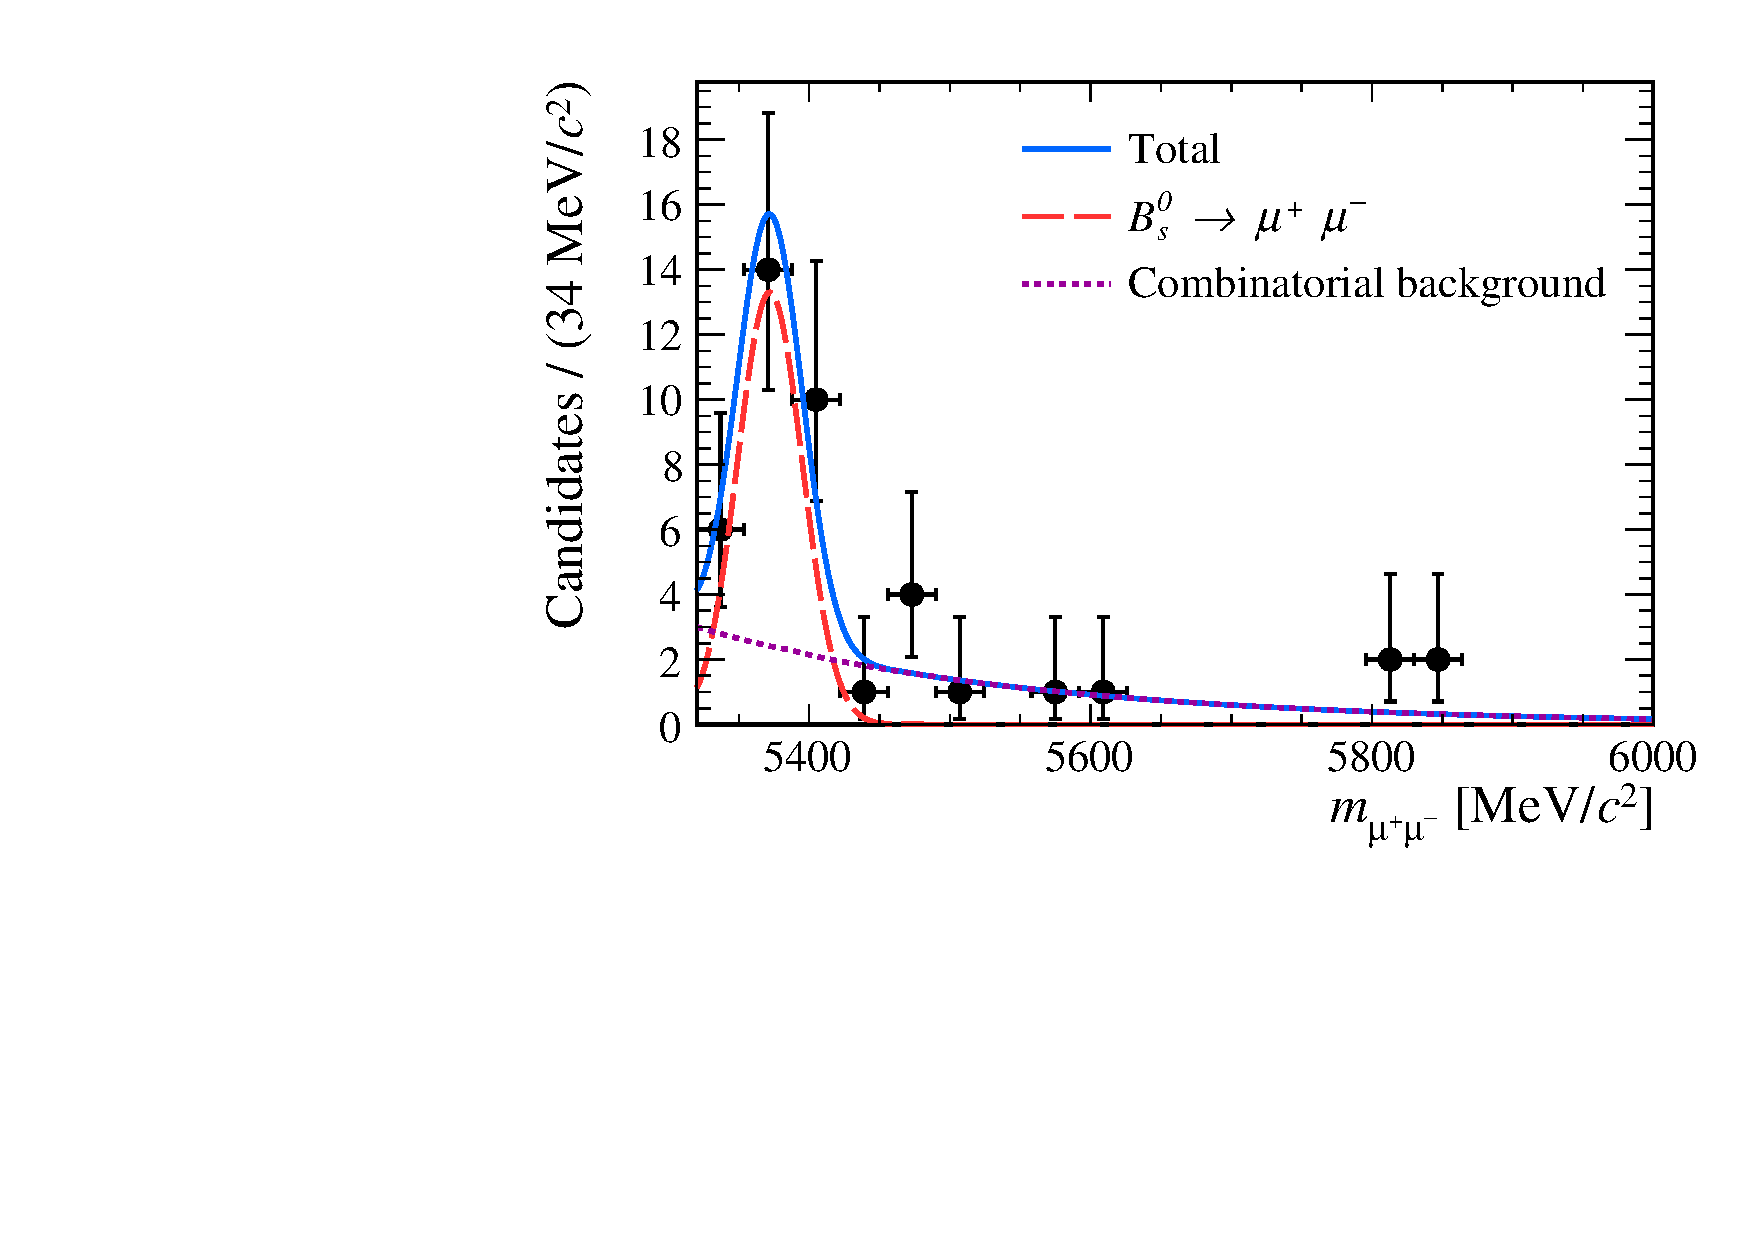
\includegraphics[width= 0.8\textwidth]{./Figs/LifetimeMeasurement/lifetime_mass_results.pdf}
            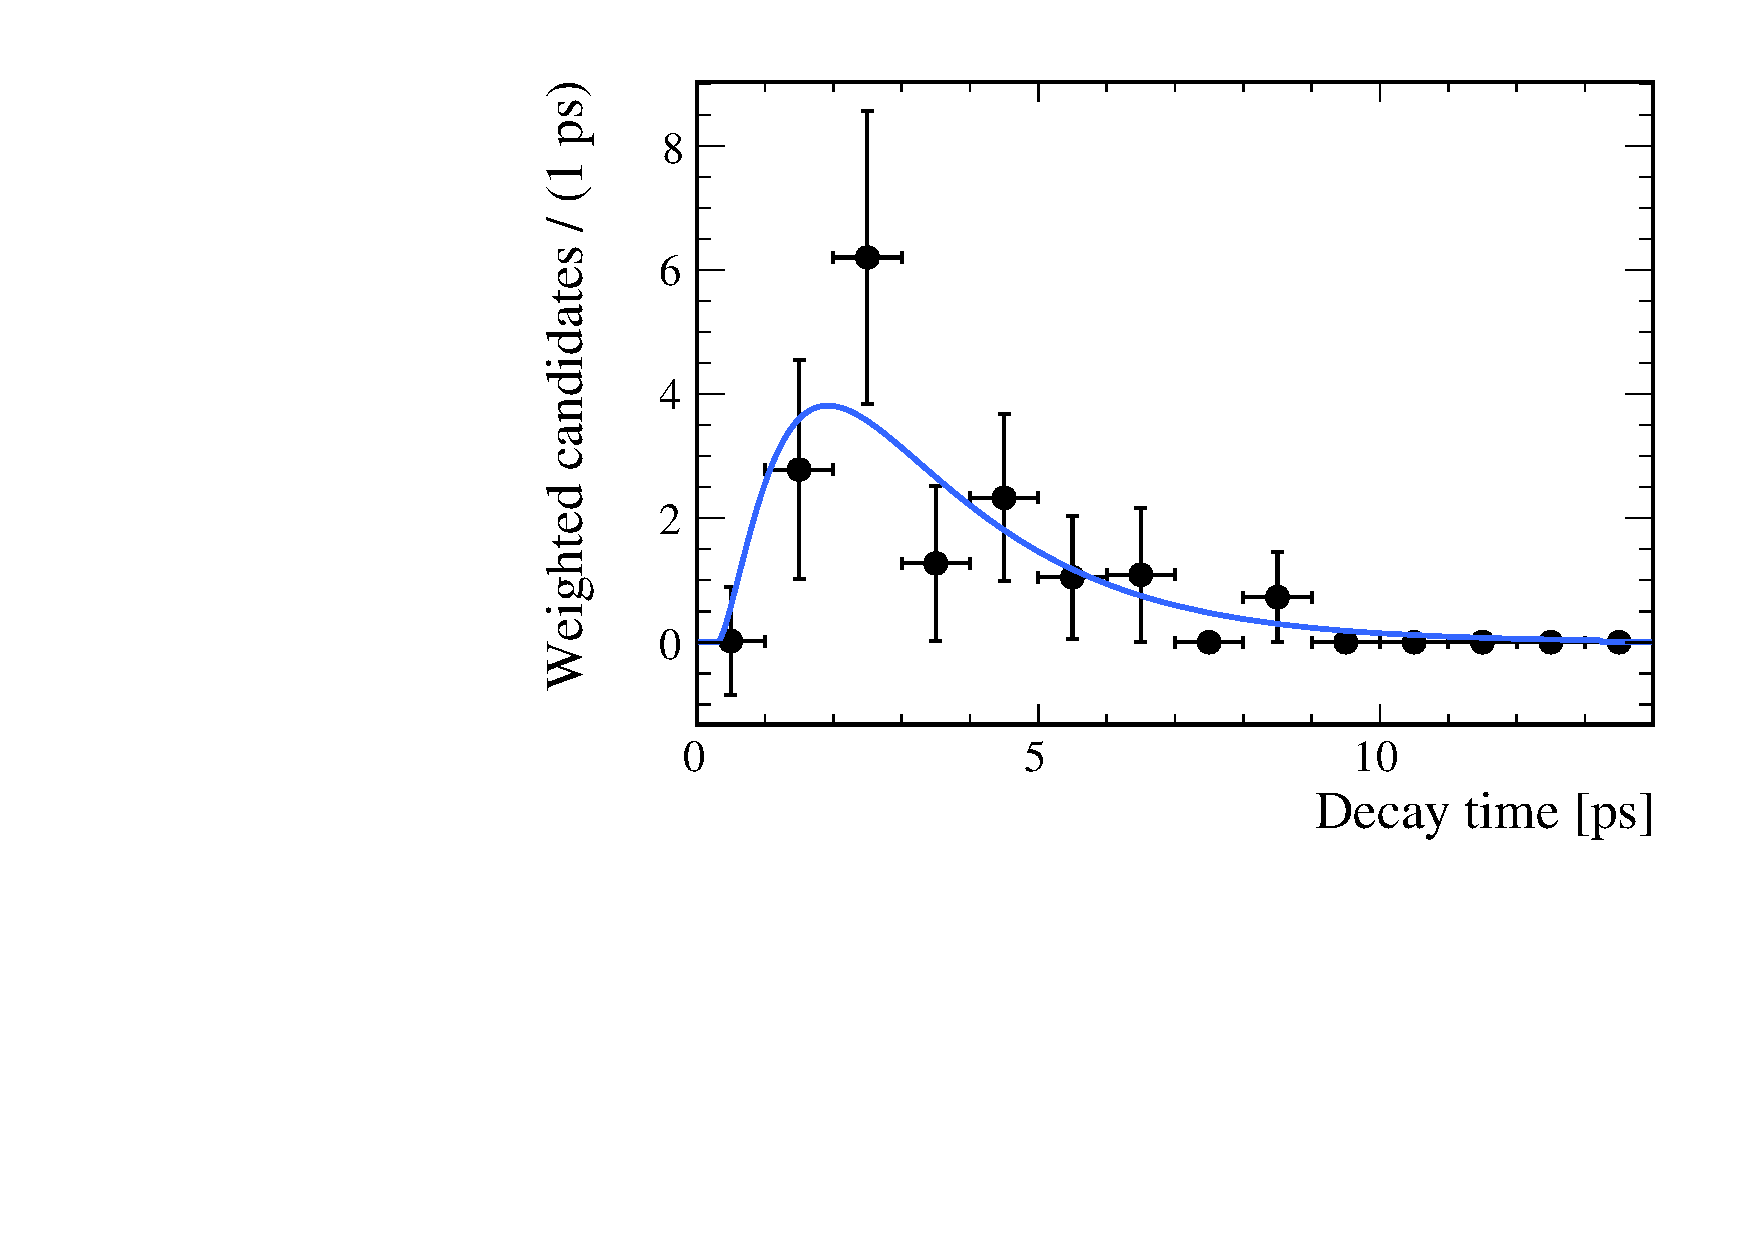
\includegraphics[width=0.8\textwidth]{./Figs/LifetimeMeasurement/lifetime_results.pdf}

    \caption{Maximum likelihood fit to the invariant mass distribution (top) and weighted decay time distribution (bottom) of \bsmumu candidates using an integrated luminosity of 4.4 \fb of data collected by the LHCb experiment. \bsmumu candidates are described by the red peak in the mass plot and combinatorial background by the blue dashed line, the total \pdf is given by the solid blue line.}
    \label{fig:ELresults}
\end{figure}



%Questions that need answering
%- where does the CBG yield and slope for the toys come from?
%- how are the lifetimes take from MC? With the acceptance?
%- What BF plots do I put in that chapter?
%- What plots should I put in here? More/less/different?
%- How does Siim get the Bs2JpisPhi yields, what triggers are applied and what is included in the mass fit and are there plots?
